% Options for packages loaded elsewhere
% Options for packages loaded elsewhere
\PassOptionsToPackage{unicode}{hyperref}
\PassOptionsToPackage{hyphens}{url}
\PassOptionsToPackage{dvipsnames,svgnames,x11names}{xcolor}
%
\documentclass[
  letterpaper,
  DIV=11,
  numbers=noendperiod]{scrreprt}
\usepackage{xcolor}
\usepackage{amsmath,amssymb}
\setcounter{secnumdepth}{5}
\usepackage{iftex}
\ifPDFTeX
  \usepackage[T1]{fontenc}
  \usepackage[utf8]{inputenc}
  \usepackage{textcomp} % provide euro and other symbols
\else % if luatex or xetex
  \usepackage{unicode-math} % this also loads fontspec
  \defaultfontfeatures{Scale=MatchLowercase}
  \defaultfontfeatures[\rmfamily]{Ligatures=TeX,Scale=1}
\fi
\usepackage{lmodern}
\ifPDFTeX\else
  % xetex/luatex font selection
\fi
%% Support for zero-width non-joiner characters.
\makeatletter
\def\zerowidthnonjoiner{%
  % Prevent ligatures and adjust kerning, but still support hyphenating.
  \texorpdfstring{%
    \TextOrMath{\nobreak\discretionary{-}{}{\kern.03em}%
      \ifvmode\else\nobreak\hskip\z@skip\fi}{}%
  }{}%
}
\makeatother
\ifPDFTeX
  \DeclareUnicodeCharacter{200C}{\zerowidthnonjoiner}
\else
  \catcode`^^^^200c=\active
  \protected\def ^^^^200c{\zerowidthnonjoiner}
\fi
%% End of ZWNJ support
% Use upquote if available, for straight quotes in verbatim environments
\IfFileExists{upquote.sty}{\usepackage{upquote}}{}
\IfFileExists{microtype.sty}{% use microtype if available
  \usepackage[]{microtype}
  \UseMicrotypeSet[protrusion]{basicmath} % disable protrusion for tt fonts
}{}
\makeatletter
\@ifundefined{KOMAClassName}{% if non-KOMA class
  \IfFileExists{parskip.sty}{%
    \usepackage{parskip}
  }{% else
    \setlength{\parindent}{0pt}
    \setlength{\parskip}{6pt plus 2pt minus 1pt}}
}{% if KOMA class
  \KOMAoptions{parskip=half}}
\makeatother
% Make \paragraph and \subparagraph free-standing
\makeatletter
\ifx\paragraph\undefined\else
  \let\oldparagraph\paragraph
  \renewcommand{\paragraph}{
    \@ifstar
      \xxxParagraphStar
      \xxxParagraphNoStar
  }
  \newcommand{\xxxParagraphStar}[1]{\oldparagraph*{#1}\mbox{}}
  \newcommand{\xxxParagraphNoStar}[1]{\oldparagraph{#1}\mbox{}}
\fi
\ifx\subparagraph\undefined\else
  \let\oldsubparagraph\subparagraph
  \renewcommand{\subparagraph}{
    \@ifstar
      \xxxSubParagraphStar
      \xxxSubParagraphNoStar
  }
  \newcommand{\xxxSubParagraphStar}[1]{\oldsubparagraph*{#1}\mbox{}}
  \newcommand{\xxxSubParagraphNoStar}[1]{\oldsubparagraph{#1}\mbox{}}
\fi
\makeatother


\usepackage{longtable,booktabs,array}
\newcounter{none} % for unnumbered tables
\usepackage{calc} % for calculating minipage widths
% Correct order of tables after \paragraph or \subparagraph
\usepackage{etoolbox}
\makeatletter
\patchcmd\longtable{\par}{\if@noskipsec\mbox{}\fi\par}{}{}
\makeatother
% Allow footnotes in longtable head/foot
\IfFileExists{footnotehyper.sty}{\usepackage{footnotehyper}}{\usepackage{footnote}}
\makesavenoteenv{longtable}
\usepackage{graphicx}
\makeatletter
\newsavebox\pandoc@box
\newcommand*\pandocbounded[1]{% scales image to fit in text height/width
  \sbox\pandoc@box{#1}%
  \Gscale@div\@tempa{\textheight}{\dimexpr\ht\pandoc@box+\dp\pandoc@box\relax}%
  \Gscale@div\@tempb{\linewidth}{\wd\pandoc@box}%
  \ifdim\@tempb\p@<\@tempa\p@\let\@tempa\@tempb\fi% select the smaller of both
  \ifdim\@tempa\p@<\p@\scalebox{\@tempa}{\usebox\pandoc@box}%
  \else\usebox{\pandoc@box}%
  \fi%
}
% Set default figure placement to htbp
\def\fps@figure{htbp}
\makeatother





\setlength{\emergencystretch}{3em} % prevent overfull lines

\providecommand{\tightlist}{%
  \setlength{\itemsep}{0pt}\setlength{\parskip}{0pt}}

\ifPDFTeX
  \TeXXeTstate=1
  \newcommand{\RL}[1]{\beginR #1\endR}
  \newcommand{\LR}[1]{\beginL #1\endL}
  \newenvironment{RTL}{\beginR}{\endR}
  \newenvironment{LTR}{\beginL}{\endL}
\fi
\ifluatex
  \newcommand{\RL}[1]{\bgroup\textdir TRT#1\egroup}
  \newcommand{\LR}[1]{\bgroup\textdir TLT#1\egroup}
  \newenvironment{RTL}{\textdir TRT\pardir TRT\bodydir TRT}{}
  \newenvironment{LTR}{\textdir TLT\pardir TLT\bodydir TLT}{}
\fi


 


\KOMAoption{captions}{tableheading}
\makeatletter
\@ifpackageloaded{bookmark}{}{\usepackage{bookmark}}
\makeatother
\makeatletter
\@ifpackageloaded{caption}{}{\usepackage{caption}}
\AtBeginDocument{%
\ifdefined\contentsname
  \renewcommand*\contentsname{Table of contents}
\else
  \newcommand\contentsname{Table of contents}
\fi
\ifdefined\listfigurename
  \renewcommand*\listfigurename{List of Figures}
\else
  \newcommand\listfigurename{List of Figures}
\fi
\ifdefined\listtablename
  \renewcommand*\listtablename{List of Tables}
\else
  \newcommand\listtablename{List of Tables}
\fi
\ifdefined\figurename
  \renewcommand*\figurename{Figure}
\else
  \newcommand\figurename{Figure}
\fi
\ifdefined\tablename
  \renewcommand*\tablename{Table}
\else
  \newcommand\tablename{Table}
\fi
}
\@ifpackageloaded{float}{}{\usepackage{float}}
\floatstyle{ruled}
\@ifundefined{c@chapter}{\newfloat{codelisting}{h}{lop}}{\newfloat{codelisting}{h}{lop}[chapter]}
\floatname{codelisting}{Listing}
\newcommand*\listoflistings{\listof{codelisting}{List of Listings}}
\makeatother
\makeatletter
\makeatother
\makeatletter
\@ifpackageloaded{caption}{}{\usepackage{caption}}
\@ifpackageloaded{subcaption}{}{\usepackage{subcaption}}
\makeatother
\usepackage{bookmark}
\IfFileExists{xurl.sty}{\usepackage{xurl}}{} % add URL line breaks if available
\urlstyle{same}
\hypersetup{
  pdftitle={تاریخچه دانشکده علوم ریاضی},
  pdfauthor={تهیه و تدوین: زهره وثاق و وحیده وحیدنیا},
  colorlinks=true,
  linkcolor={blue},
  filecolor={Maroon},
  citecolor={Blue},
  urlcolor={Blue},
  pdfcreator={LaTeX via pandoc}}


\title{تاریخچه دانشکده علوم ریاضی}
\usepackage{etoolbox}

\usepackage{xepersian}
\settextfont{Gandom}
\setlatintextfont{Times New Roman}

\makeatletter
\providecommand{\subtitle}[1]{% add subtitle to \maketitle
  \apptocmd{\@title}{\par {\large #1 \par}}{}{}
}
\makeatother
\subtitle{دانشگاه فردوسی مشهد}
\author{تهیه و تدوین: زهره وثاق و وحیده وحیدنیا}
\date{Invalid Date}
\begin{document}
\maketitle

\renewcommand*\contentsname{Table of contents}
{
\setcounter{tocdepth}{2}
\tableofcontents
}

\bookmarksetup{startatroot}

\chapter{تاریخچه دانشکده علوم
ریاضی}\label{ux62aux627ux631ux6ccux62eux686ux647-ux62fux627ux646ux634ux6a9ux62fux647-ux639ux644ux648ux645-ux631ux6ccux627ux636ux6cc}

دانشگاه فردوسی مشهد

\hfill\break

زیر نظر هیئت رییسه دانشکده علوم ریاضی

تهیه و تدوین: زهره وثاق و وحیده وحیدنیا --- تیر ماه ۱۴۰۵

\bookmarksetup{startatroot}

\chapter{پیشگفتار}\label{ux67eux6ccux634ux6afux641ux62aux627ux631}

\bookmarksetup{startatroot}

\chapter{تاریخچه
دانشکده}\label{ux62aux627ux631ux6ccux62eux686ux647-ux62fux627ux646ux634ux6a9ux62fux647}

\bookmarksetup{startatroot}

\chapter{تاریخچه
دانشکده}\label{ux62aux627ux631ux6ccux62eux686ux647-ux62fux627ux646ux634ux6a9ux62fux647-1}

گروه ریاضی یکی از قدیمی‌ترین گروه‌های آموزشی دانشگاه می‌باشد که در سال ۱۳۴۱
به همت استادانی چون دکتر اسماعیل بیگی (رئیس وقت دانشگاه مشهد) و دکتر
محمدعلی سعادت (اولین رئیس دانشکده علوم) به عنوان اولین رشته در دانشکده
علوم تحت عنوان «ریاضی -- فیزیک» پایه‌ریزی گردید. گروه ریاضی تا سال ۱۳۴۳
به صورت دوره‌های سه ساله در رشته ریاضی-فیزیک دانشجو تربیت می‌کرد. در سال
۱۳۴۴ این رشته به «ریاضی و آمار» تغییر نام داد. دانشجویان طی یک دوره چهار
ساله با درجه کارشناسی ریاضی فارغ‌التحصیل می‌شدند. در این دوران پروفسور تقی
فاطمی در چندین دوره مدیریت گروه ریاضی را بر عهده داشتند. گروه ریاضی
اولین گروه آموزشی دانشگاه فردوسی مشهد است که بعد از پیروزی انقلاب اسلامی
ایران، دانشجوی دکتری پذیرفته است. دوره‌های کارشناسی ارشد ریاضی و آمار به
ترتیب در سال‌های ۱۳۶۴ و ۱۳۶۶ و دوره‌های دکتری ریاضی و آمار به ترتیب در
سال‌های ۱۳۶۹ و ۱۳۷۳ ایجاد شدند.

تأسیس دانشکده علوم ریاضی در سال ۱۳۷۵

با رشد گروه ریاضی، متعاقباً رشته آمار و ماشین‌های حسابگر در این گروه شروع
به فعالیت نمود. از سال ۱۳۵۷ تا ۱۳۶۱ مرکز کامپیوتر دانشگاه نیز زیر نظر
گروه ریاضی فعالیت داشت. این گروه آموزشی تا سال ۱۳۶۷ تحت نام «گروه ریاضی،
آمار و کامپیوتر» به فعالیت خود ادامه داد. از این سال به بعد به دو گروه
آموزشی ریاضی و آمار تفکیک شد. رشته کامپیوتر نیز تا چندین سال مشترکاً با
گروه ریاضی فعالیت می‌نمود که در سال ۱۳۷۱ به دانشکده مهندسی منتقل گردید.
با دوراندیشی اعضای هیأت علمی وقت و پیگیری دکتر محمدرضا رجب‌زاده مقدم (که
طی حکمی از طرف رئیس وقت دانشگاه مسئول پیگیری تأسیس دانشکده علوم ریاضی
شده بود)، بالاخره در سال ۱۳۷۵، وزارت علوم موافقت خود را با تأسیس دانشکده
علوم ریاضی اعلام نمود و این دانشکده با تفکیک از دانشکده علوم پایه و با
دو گروه آموزشی ریاضی و آمار و ۴۸ عضو هیأت علمی تأسیس شد.

گروه‌های آمار و ریاضی این دانشکده از سال ۱۳۸۰ تا کنون به ترتیب به عنوان
قطب‌های علمی آمار و ریاضی کشور شناخته شده‌اند. گروه آموزشی ریاضی در سال
تحصیلی ۱۳۸۶-۱۳۸۷ به دو گروه «ریاضی کاربردی» و «ریاضی محض» تقسیم گردید.
در سال ۱۳۹۸، دوره کارشناسی علوم کامپیوتر و دوره کارشناسی ارشد گرایش
ریاضیات زیستی تأسیس گردید. در سال ۱۴۰۴ گروه ریاضی علوم کامپیوتر در
دانشکده راه‌اندازی شد و همچنین در همین سال اولین دوره از دانشجویان
کارشناسی ارشد علوم کامپیوتر پذیرش گردیدند.

دانشکده علوم ریاضی در راستای اهداف دانشگاه فردوسی مشهد و وزارت علوم،
تحقیقات و فناوری در سه حوزه آموزش، پژوهش و کارآفرینی فعالیت دارد. این
دانشکده به تربیت دانشجو در سه مقطع کارشناسی، کارشناسی ارشد و دکترا در
چهار رشته اصلی ریاضی محض، ریاضی کاربردی، آمار و علوم کامپیوتر می‌پردازد.

\begin{figure}[H]

{\centering \pandocbounded{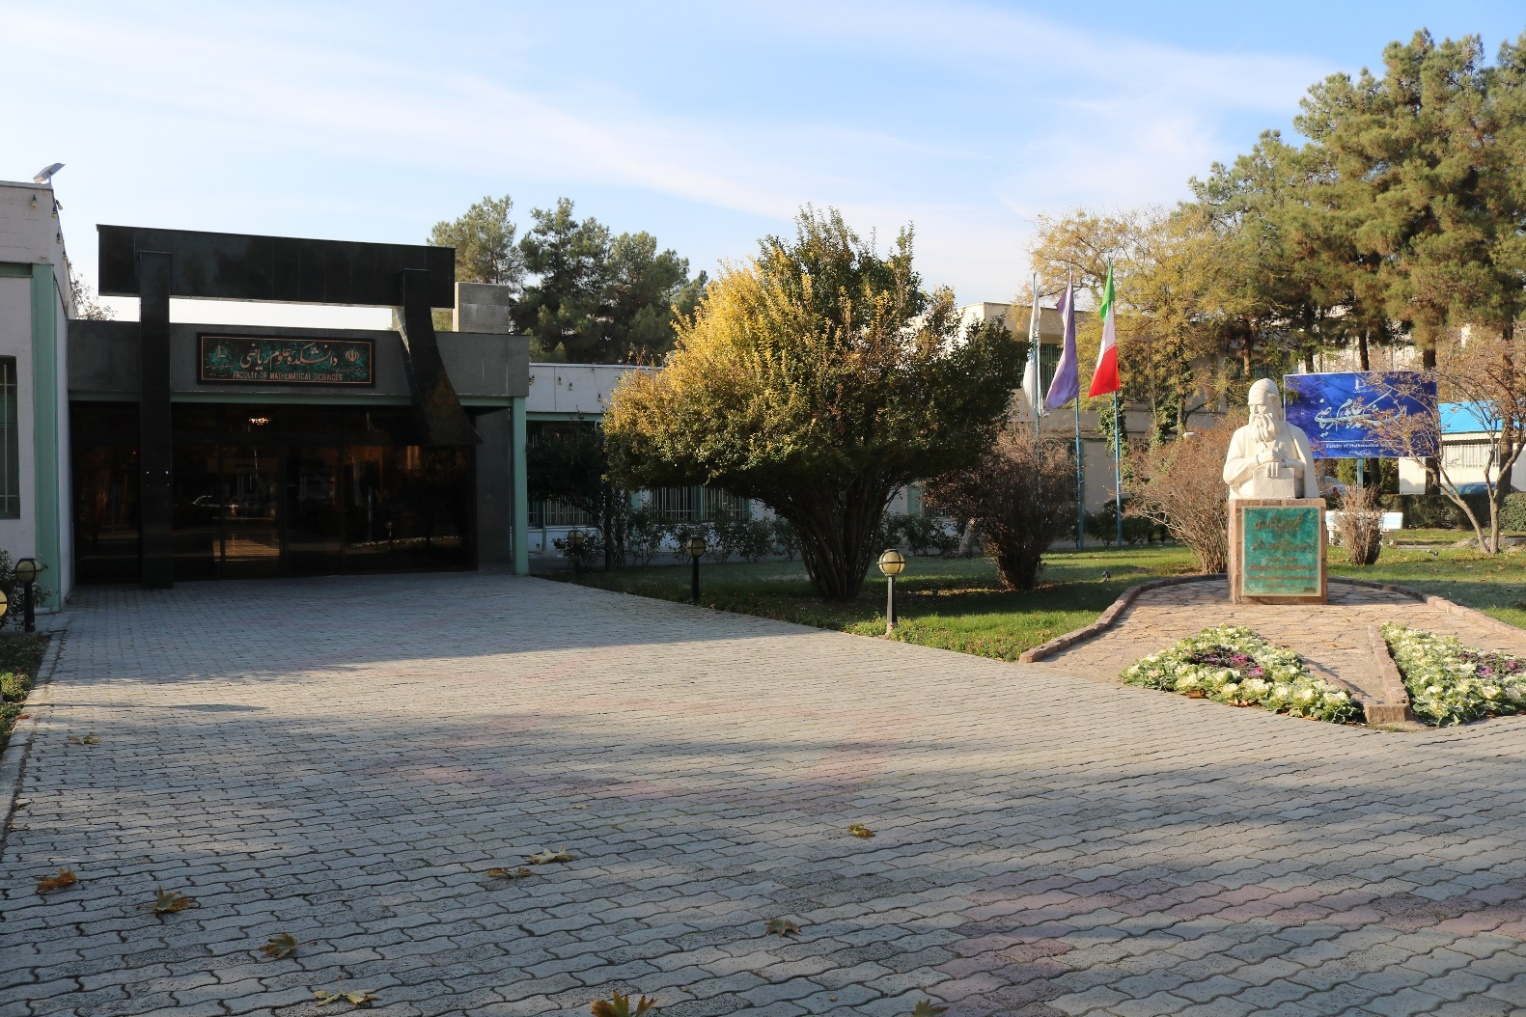
\includegraphics[keepaspectratio]{images/img_007.jpeg}}

}

\caption{image}

\end{figure}%

\begin{figure}[H]

{\centering \pandocbounded{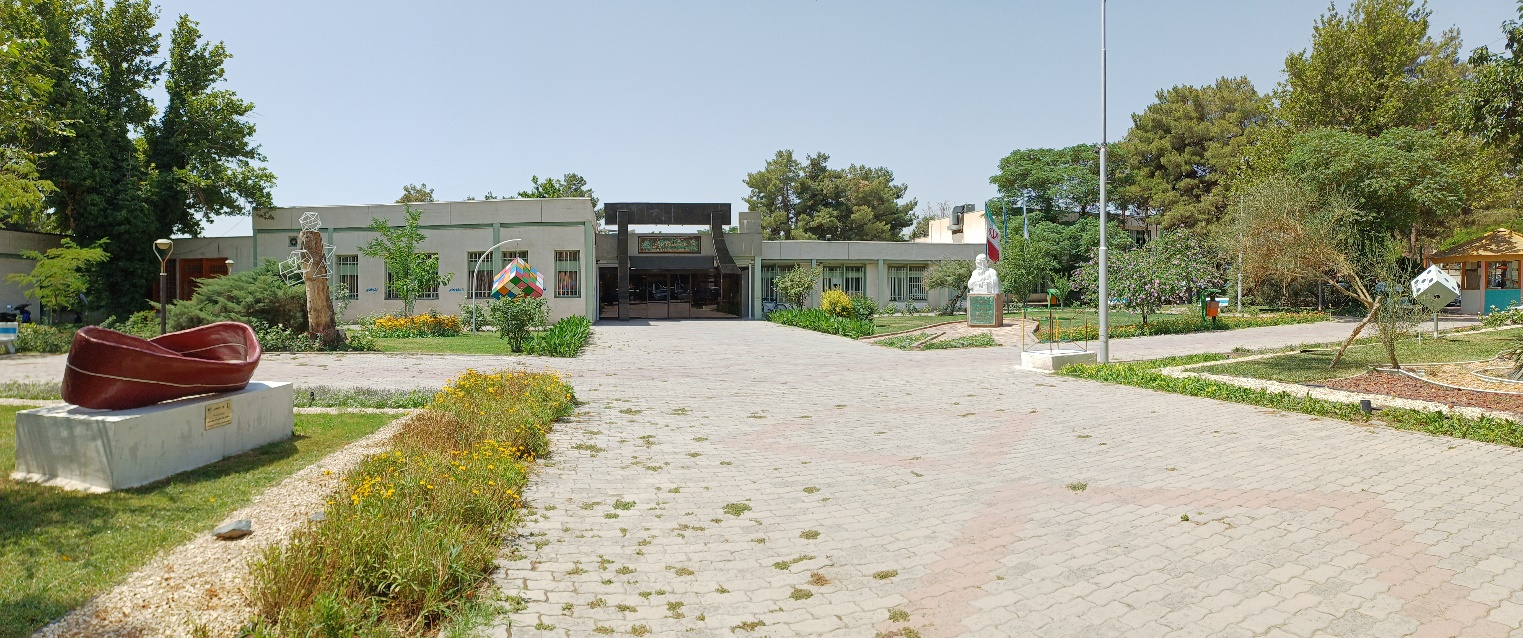
\includegraphics[keepaspectratio]{images/img_019.jpeg}}

}

\caption{image}

\end{figure}%

\bookmarksetup{startatroot}

\chapter{روسای
دانشکده}\label{ux631ux648ux633ux627ux6cc-ux62fux627ux646ux634ux6a9ux62fux647}

\bookmarksetup{startatroot}

\chapter{روسای دانشکده از آغاز
تاکنون}\label{ux631ux648ux633ux627ux6cc-ux62fux627ux646ux634ux6a9ux62fux647-ux627ux632-ux622ux63aux627ux632-ux62aux627ux6a9ux646ux648ux646}

\bookmarksetup{startatroot}

\chapter{مدیران و
معاونان}\label{ux645ux62fux6ccux631ux627ux646-ux648-ux645ux639ux627ux648ux646ux627ux646}

\bookmarksetup{startatroot}

\chapter{معاونین پژوهش و فناوری دانشکده از آغاز
تاکنون}\label{ux645ux639ux627ux648ux646ux6ccux646-ux67eux698ux648ux647ux634-ux648-ux641ux646ux627ux648ux631ux6cc-ux62fux627ux646ux634ux6a9ux62fux647-ux627ux632-ux622ux63aux627ux632-ux62aux627ux6a9ux646ux648ux646}

\bookmarksetup{startatroot}

\chapter{معاونان آموزشی و فرهنگی دانشکده از آغاز
تاکنون}\label{ux645ux639ux627ux648ux646ux627ux646-ux622ux645ux648ux632ux634ux6cc-ux648-ux641ux631ux647ux646ux6afux6cc-ux62fux627ux646ux634ux6a9ux62fux647-ux627ux632-ux622ux63aux627ux632-ux62aux627ux6a9ux646ux648ux646}

\bookmarksetup{startatroot}

\chapter{معاونان اداری و مالی دانشکده از آغاز تا سال
۱۳۹۰}\label{ux645ux639ux627ux648ux646ux627ux646-ux627ux62fux627ux631ux6cc-ux648-ux645ux627ux644ux6cc-ux62fux627ux646ux634ux6a9ux62fux647-ux627ux632-ux622ux63aux627ux632-ux62aux627-ux633ux627ux644-ux6f1ux6f3ux6f9ux6f0}

\bookmarksetup{startatroot}

\chapter{گروه‌های
آموزشی}\label{ux6afux631ux648ux647ux647ux627ux6cc-ux622ux645ux648ux632ux634ux6cc}

\bookmarksetup{startatroot}

\chapter{معرفی گروه‌های آموزشی، مدیران گروه، رشته‌ها و گرایش‌های
موجود}\label{ux645ux639ux631ux641ux6cc-ux6afux631ux648ux647ux647ux627ux6cc-ux622ux645ux648ux632ux634ux6cc-ux645ux62fux6ccux631ux627ux646-ux6afux631ux648ux647-ux631ux634ux62aux647ux647ux627-ux648-ux6afux631ux627ux6ccux634ux647ux627ux6cc-ux645ux648ux62cux648ux62f}

\section{گروه آموزشی
ریاضی}\label{ux6afux631ux648ux647-ux622ux645ux648ux632ux634ux6cc-ux631ux6ccux627ux636ux6cc}

این گروه در سال تحصیلی ۱۳۸۶-۱۳۸۷ به دو گروه ریاضی کاربردی و محض تقسیم
گردید.

\subsection{مدیران گروه آموزشی ریاضی از سال ۱۳۵۵ تا
۱۳۸۶}\label{ux645ux62fux6ccux631ux627ux646-ux6afux631ux648ux647-ux622ux645ux648ux632ux634ux6cc-ux631ux6ccux627ux636ux6cc-ux627ux632-ux633ux627ux644-ux6f1ux6f3ux6f5ux6f5-ux62aux627-ux6f1ux6f3ux6f8ux6f6}

{\def\LTcaptype{none} % do not increment counter
\begin{longtable}[]{@{}lll@{}}
\toprule\noalign{}
نام و نام خانوادگی & مرتبه علمی در دوران تصدی & دوره تصدی \\
\midrule\noalign{}
\endhead
\bottomrule\noalign{}
\endlastfoot
پروفسور تقی فاطمی & استاد & ۱۳۵۵ تا ۱۳۵۵ \\
دکتر بهمن هنری & استادیار & ۱۳۵۵ تا ۱۳۵۷ \\
دکتر اسدالله نیکنام & استادیار & ۱۳۵۷ تا ۱۳۶۱ \\
دکتر باقر نشوادیان & استادیار & ۱۳۶۱ تا ۱۳۶۳ \\
دکتر علی انصاری & استادیار & ۱۳۶۳ تا ۱۳۶۴ \\
دکتر محمدرضا رجب‌زاده مقدم & دانشیار & ۱۳۶۴ تا ۱۳۶۸ \\
دکتر اسدالله نیکنام & دانشیار & ۱۳۶۸ تا ۱۳۶۹ \\
دکتر اصغر کرایه‌چیان & استادیار & ۱۳۶۹ تا ۱۳۷۲ \\
دکتر محمود یاسی & استادیار & ۱۳۷۲ تا ۱۳۷۲ \\
دکتر اسدالله نیکنام & استاد & ۱۳۷۲ تا ۱۳۷۴ \\
دکتر محمدعلی پور عبدالله & استاد & ۱۳۷۴ تا ۱۳۷۶ \\
دکتر علی وحیدیان کامیاد & دانشیار & ۱۳۷۶ تا ۱۳۷۷ \\
دکتر فائزه توتونیان & استاد & ۱۳۷۷ تا ۱۳۷۹ \\
دکتر اسدالله نیکنام & استاد & ۱۳۷۹ تا ۱۳۸۱ \\
دکتر شیرین حجازیان & استادیار & ۱۳۸۲ تا ۱۳۸۳ \\
دکتر فاطمه هلن قانع استاد قاسمی & دانشیار & ۱۳۸۳ تا ۱۳۸۵ \\
دکتر زهرا افشارنژاد & استاد & ۱۳۸۵ تا ۱۳۸۶ \\
\end{longtable}
}

\section{گروه آموزشی ریاضی
کاربردی}\label{ux6afux631ux648ux647-ux622ux645ux648ux632ux634ux6cc-ux631ux6ccux627ux636ux6cc-ux6a9ux627ux631ux628ux631ux62fux6cc}

گروه ریاضی کاربردی در سال ۱۳۸۶ از گروه ریاضی محض جدا شد. دانشجویان این
رشته‌ها ضمن آشنایی با مفاهیم ریاضی، کاربرد ریاضیات را آموزش می‌بینند و
روش‌ها و تکنیک‌های علمی را به منظور حل مسائل واقعی در زندگی روزمره فرا
می‌گیرند. قطب علمی مدلسازی و کنترل دستگاه‌ها و مرکز پژوهشی شیوه‌های تدریس
آموزش ریاضی، آزمایشگاه‌های فناورانه طراحی و تولید بازی‌های رایانه‌ای و
آزمایشگاه بهینه‌سازی در این گروه فعال هستند. همچنین انتشار مجله
علمی-پژوهشی «ایرانی آنالیز عددی و بهینه‌سازی» نیز از جمله فعالیت‌های این
گروه می‌باشد.

\subsection{دوره
کارشناسی}\label{ux62fux648ux631ux647-ux6a9ux627ux631ux634ux646ux627ux633ux6cc}

تا قبل از سال ۱۳۹۰ این گروه مجری دوره کارشناسی ریاضی کاربردی بوده که هدف
از این دوره افزون بر تربیت کارشناسان مورد نیاز ادارات، سازمان‌های دولتی و
خصوصی همچون بانک‌ها، تربیت افرادی برای انتقال علوم ریاضی و کاربرد
کامپیوتر به دانشجویان برای مدل‌سازی سیستم‌ها، استنباط، تجزیه و تحلیل انواع
سیستم‌های علمی و کاربردی، بهینه‌سازی سیستم‌ها و همچنین کاربرد تحقیق در
عملیات و بهینه‌سازی در صنایع و سازمان‌های خدماتی است. این گروه در دوره
کارشناسی از سال ۱۳۹۰ در رشته ریاضیات و کاربردها به طور مشترک با گروه
ریاضی محض دانشجو می‌پذیرد.

\subsection{دوره تحصیلات
تکمیلی}\label{ux62fux648ux631ux647-ux62aux62dux635ux6ccux644ux627ux62a-ux62aux6a9ux645ux6ccux644ux6cc}

گروه ریاضی کاربردی افزون بر دانشجویان کارشناسی، دانشجوی کارشناسی ارشد و
دانشجوی دکتری نیز دارد. برنامه کارشناسی ارشد در سال ۱۳۷۰ تأسیس شده است.
زمینه‌های تخصصی این مقطع عبارتند از: آنالیز عددی، تحقیق در عملیات، کنترل
و بهینه‌سازی، معادلات دیفرانسیل کاربردی، نظریه گراف و آموزش ریاضی،
مدلسازی در علوم زیستی و پزشکی، هوش محاسباتی. این گروه از سال ۱۳۷۳
دانشجوی دکتری پذیرفته است.

\subsection{مدیران گروه آموزشی ریاضی
کاربردی}\label{ux645ux62fux6ccux631ux627ux646-ux6afux631ux648ux647-ux622ux645ux648ux632ux634ux6cc-ux631ux6ccux627ux636ux6cc-ux6a9ux627ux631ux628ux631ux62fux6cc}

{\def\LTcaptype{none} % do not increment counter
\begin{longtable}[]{@{}lll@{}}
\toprule\noalign{}
نام و نام خانوادگی & مرتبه علمی در دوران تصدی & دوره تصدی \\
\midrule\noalign{}
\endhead
\bottomrule\noalign{}
\endlastfoot
دکتر زهرا افشارنژاد & استاد & ۱۳۸۶ تا ۱۳۸۷ \\
دکتر فریدون رهبرنیا & استادیار & ۱۳۸۷ تا ۱۳۸۹ \\
دکتر مرتضی گچ‌پزان & استادیار - دانشیار & ۱۳۸۹ تا ۱۳۹۳ \\
دکتر سهراب عفتی & استاد & ۱۳۹۳ تا ۱۳۹۴ \\
دکتر مرتضی گچ‌پزان & دانشیار & ۱۳۹۴ تا ۱۳۹۶ \\
دکتر سهراب عفتی & استاد & ۱۳۹۶ تا ۱۴۰۱ \\
دکتر مرتضی گچ‌پزان & دانشیار & ۱۴۰۱ تا ۱۴۰۳ \\
دکتر مصطفی توکلی & دانشیار- استاد & ۱۴۰۳ تاکنون \\
\end{longtable}
}

\section{اعضاء هیأت علمی گروه آموزشی ریاضی
کاربردی}\label{ux627ux639ux636ux627ux621-ux647ux6ccux623ux62a-ux639ux644ux645ux6cc-ux6afux631ux648ux647-ux622ux645ux648ux632ux634ux6cc-ux631ux6ccux627ux636ux6cc-ux6a9ux627ux631ux628ux631ux62fux6cc}

{\def\LTcaptype{none} % do not increment counter
\begin{longtable}[]{@{}
  >{\raggedright\arraybackslash}p{(\linewidth - 8\tabcolsep) * \real{0.2000}}
  >{\raggedright\arraybackslash}p{(\linewidth - 8\tabcolsep) * \real{0.2000}}
  >{\raggedright\arraybackslash}p{(\linewidth - 8\tabcolsep) * \real{0.2000}}
  >{\raggedright\arraybackslash}p{(\linewidth - 8\tabcolsep) * \real{0.2000}}
  >{\raggedright\arraybackslash}p{(\linewidth - 8\tabcolsep) * \real{0.2000}}@{}}
\toprule\noalign{}
\begin{minipage}[b]{\linewidth}\raggedright
ردیف
\end{minipage} & \begin{minipage}[b]{\linewidth}\raggedright
نام و نام خانوادگی
\end{minipage} & \begin{minipage}[b]{\linewidth}\raggedright
مرتبه علمی
\end{minipage} & \begin{minipage}[b]{\linewidth}\raggedright
تاریخ شروع همکاری
\end{minipage} & \begin{minipage}[b]{\linewidth}\raggedright
تاریخ آخرین ارتقا
\end{minipage} \\
\midrule\noalign{}
\endhead
\bottomrule\noalign{}
\endlastfoot
۱ & دکتر مصطفی توکلی & استاد & ۲۴/۱۲/۱۳۹۳ & ۱۴/۰۹/۱۴۰۴ \\
۲ & دکتر فریدون رهبرنیا & استاد & ۲۹/۰۹/۱۳۷۱ & ۰۳/۱۲/۱۴۰۴ \\
۳ & دکتر علیرضا سهیلی & استاد & انتقال۳۰/۰۹/۱۳۸۸ & ۱۰/۰۷/۱۳۸۸ \\
۴ & دکتر سهراب عفتی & استاد & انتقال۰۱/۰۷/۱۳۸۷ & ۲۳/۱۰/۱۳۹۳ \\
۵ & دکتر رضا قنبری & استاد & ۲۵/۰۳/۱۳۸۹ & ۲۶/۰۵/۱۴۰۴ \\
۶ & دکتر امید سلیمانی فرد & دانشیار & انتقال۱۶/۱۱/۱۳۹۳ & ۳۱/۰۲/۱۳۹۰ \\
۷ & دکتر محمد شهروزی & دانشیار & انتقال۰۱/۱۱/۱۴۰۲ & ۰۱/۱۰/۱۴۰۱ \\
۸ & دکتر مرتضی گچ پزان & دانشیار & انتقال۰۱/۱۱/۱۳۸۵ & ۱۸/۰۲/۱۳۹۲ \\
۹ & دکتر مصطفی جانی & استادیار & حق التدریس & - \\
۱۰ & دکتر مهدی رنجبر تقی آباد & استادیار & ۱۲/۰۷/۱۴۰۴ & - \\
۱۱ & دکتر اصغر قربانی & استادیار & ۰۱/۰۶/۱۳۹۴ & - \\
۱۲ & دکتر امین منصوری & استادیار & ۳۰/۰۵/۱۴۰۳ & - \\
۱۳ & دکتر سیدمحسن میری & استادیار & ۲۱/۰۷/۱۴۰۴ & - \\
۱۴ & دکتر فائزه رضوان فرد & & حق التدریس & - \\
\end{longtable}
}

\section{اعضاء هیأت علمی بازنشسته گروه آموزشی ریاضی
کاربردی}\label{ux627ux639ux636ux627ux621-ux647ux6ccux623ux62a-ux639ux644ux645ux6cc-ux628ux627ux632ux646ux634ux633ux62aux647-ux6afux631ux648ux647-ux622ux645ux648ux632ux634ux6cc-ux631ux6ccux627ux636ux6cc-ux6a9ux627ux631ux628ux631ux62fux6cc}

{\def\LTcaptype{none} % do not increment counter
\begin{longtable}[]{@{}
  >{\raggedright\arraybackslash}p{(\linewidth - 8\tabcolsep) * \real{0.2000}}
  >{\raggedright\arraybackslash}p{(\linewidth - 8\tabcolsep) * \real{0.2000}}
  >{\raggedright\arraybackslash}p{(\linewidth - 8\tabcolsep) * \real{0.2000}}
  >{\raggedright\arraybackslash}p{(\linewidth - 8\tabcolsep) * \real{0.2000}}
  >{\raggedright\arraybackslash}p{(\linewidth - 8\tabcolsep) * \real{0.2000}}@{}}
\toprule\noalign{}
\begin{minipage}[b]{\linewidth}\raggedright
ردیف
\end{minipage} & \begin{minipage}[b]{\linewidth}\raggedright
نام و نام خانوادگی
\end{minipage} & \begin{minipage}[b]{\linewidth}\raggedright
مرتبه علمی
\end{minipage} & \begin{minipage}[b]{\linewidth}\raggedright
تاریخ شروع همکاری
\end{minipage} & \begin{minipage}[b]{\linewidth}\raggedright
تاریخ بازنشستگی
\end{minipage} \\
\midrule\noalign{}
\endhead
\bottomrule\noalign{}
\endlastfoot
۱ & دکتر زهرا افشارنژاد & استاد & ۰۹/۰۸/۱۳۵۶ & ۲۸/۱۲/۱۳۸۹ \\
۲ & دکتر فائزه توتونیان & استاد & ۱۸/۱۱/۱۳۵۴ & ۰۱/۰۷/۱۳۹۲ \\
۳ & دکتر جعفر صابری نجفی & استاد & ۰۵/۱۲/۱۳۶۱ & ۰۱/۰۷/۱۳۹۰ \\
۴ & دکتر سید حسن علم الهدایی & استاد & ۰۱/۰۷/۱۳۷۸ & ۱۵/۰۶/۱۴۰۴ \\
۵ & دکتر محمد هادی فراهی & استاد & انتقال۰۴/۰۸/۱۳۶۴ & ۰۱/۱۱/۱۳۹۰ \\
۶ & دکتر اصغر کرایه‌چیان & استاد & ۱۴/۰۷/۱۳۴۷ & ۰۱/۰۷/۱۳۸۷ \\
۷ & دکتر علی وحیدیان کامیاد & استاد & ۲۸/۱۰/۱۳۵۱ & ۰۱/۱۱/۱۳۹۰ \\
۸ & دکتر حسین تقی زاده کاخکی & دانشیار & ۲۵/۰۶/۱۳۷۲ & ۲۹/۱۲/۱۳۹۶ \\
۹ & آقای عطااله زارع & دانشور & ۱۷/۰۳/۱۳۶۱ & ۰۱/۰۷/۱۳۸۴ \\
۱۰ & آقای سید حسین اورعی & مربی & ۲۰/۰۸/۱۳۶۰ & ۰۱/۰۷/۱۳۸۶ \\
۱۱ & آقای مسعود ببر حسینی & مربی & ۰۵/۱۰/۱۳۵۶ & ۰۱/۰۷/۱۳۸۷ \\
۱۲ & آقای ابوالفضل حاجی زاده & مربی & ۲۲/۱۱/۱۳۵۴ & ۰۱/۰۷/۱۳۸۳ \\
\end{longtable}
}

\section{گروه آموزشی ریاضی
محض}\label{ux6afux631ux648ux647-ux622ux645ux648ux632ux634ux6cc-ux631ux6ccux627ux636ux6cc-ux645ux62dux636}

گروه ریاضی محض در سال ۱۳۸۶ به عنوان یک گروه مستقل آغاز به کار نمود. این
گروه در دوره کارشناسی ریاضیات و کاربردها با کهادهای آنالیز، جبر و هندسه،
دوره‌های کارشناسی ارشد و دکتری در گرایش‌های آنالیز (آنالیز تابعی، آنالیز
هارمونیک، نظریه عملگرها)، جبر (نظریه گروه‌ها، جبر جابجایی، گراف و
ترکیبیات، نظریه کدگذاری) و هندسه (سیستم‌های دینامیکی، توپولوژی جبری)
فعالیت می‌نماید. قطب علمی «آنالیز روی ساختارهای جبری» یکی از اولین قطب‌های
مصوب وزارت عتف در سطح کشور بوده که در این گروه فعال است. این گروه مجله
پژوهشی «ریاضی خیام» را به زبان انگلیسی منتشر می‌کند که در سال ۱۳۹۸ در
Scopus نمایه شد.

\subsection{دوره
کارشناسی}\label{ux62fux648ux631ux647-ux6a9ux627ux631ux634ux646ux627ux633ux6cc-1}

هدف این دوره، تربیت دبیران ریاضی در آموزش و پرورش، تربیت کارشناس مورد
نیاز برخی از ادارات و ارگان‌های دولتی، تربیت افراد برای استفاده از علوم
ریاضی در مدل‌سازی سیستم‌ها در سایر علوم (فیزیک، مهندسی، اقتصاد)، گسترش
مرزهای دانش و ایجاد روحیه علمی در جامعه است.

\subsection{دوره تحصیلات
تکمیلی}\label{ux62fux648ux631ux647-ux62aux62dux635ux6ccux644ux627ux62a-ux62aux6a9ux645ux6ccux644ux6cc-1}

در گروه ریاضی محض دانشجوی کارشناسی ارشد و دانشجوی دکتری مشغول به تحصیل
هستند. برنامه کارشناسی ارشد در سال ۱۳۶۴ تأسیس شد و بر آنالیز تابعی،
آنالیز هارمونیک، توپولوژی جبری، سیستم‌های دینامیکی، نظریه گروه‌ها، نظریه
حلقه‌ها و ترکیبیات جبری متمرکز است. دوره دکتری این رشته در سال ۱۳۶۹ تأسیس
شد.

\subsection{مدیران گروه آموزشی ریاضی
محض}\label{ux645ux62fux6ccux631ux627ux646-ux6afux631ux648ux647-ux622ux645ux648ux632ux634ux6cc-ux631ux6ccux627ux636ux6cc-ux645ux62dux636}

{\def\LTcaptype{none} % do not increment counter
\begin{longtable}[]{@{}lll@{}}
\toprule\noalign{}
نام و نام خانوادگی & مرتبه علمی در دوران تصدی & دوره تصدی \\
\midrule\noalign{}
\endhead
\bottomrule\noalign{}
\endlastfoot
دکتر شیرین حجازیان & دانشیار & ۱۳۸۷ تا ۱۳۸۹ \\
دکتر رجبعلی کامیابی گل & استاد & ۱۳۸۹ تا ۱۳۹۱ \\
دکتر بهروز مشایخی‌فرد & استاد & ۱۳۹۱ تا ۱۳۹۵ \\
دکتر محمد جانفدا & دانشیار & ۱۳۹۵ تا ۱۳۹۹ \\
دکتر رجبعلی کامیابی گل & استاد & ۱۳۹۹ تا ۱۴۰۱ \\
دکتر فاطمه هلن قانع استاد قاسمی & استاد & ۱۴۰۱ تا ۱۴۰۳ \\
دکتر کاظم خشیارمنش & استاد & ۱۴۰۳ تاکنون \\
\end{longtable}
}

\section{اعضاء هیأت علمی گروه آموزشی ریاضی
محض}\label{ux627ux639ux636ux627ux621-ux647ux6ccux623ux62a-ux639ux644ux645ux6cc-ux6afux631ux648ux647-ux622ux645ux648ux632ux634ux6cc-ux631ux6ccux627ux636ux6cc-ux645ux62dux636}

{\def\LTcaptype{none} % do not increment counter
\begin{longtable}[]{@{}
  >{\raggedright\arraybackslash}p{(\linewidth - 8\tabcolsep) * \real{0.2000}}
  >{\raggedright\arraybackslash}p{(\linewidth - 8\tabcolsep) * \real{0.2000}}
  >{\raggedright\arraybackslash}p{(\linewidth - 8\tabcolsep) * \real{0.2000}}
  >{\raggedright\arraybackslash}p{(\linewidth - 8\tabcolsep) * \real{0.2000}}
  >{\raggedright\arraybackslash}p{(\linewidth - 8\tabcolsep) * \real{0.2000}}@{}}
\toprule\noalign{}
\begin{minipage}[b]{\linewidth}\raggedright
ردیف
\end{minipage} & \begin{minipage}[b]{\linewidth}\raggedright
نام و نام خانوادگی
\end{minipage} & \begin{minipage}[b]{\linewidth}\raggedright
مرتبه علمی
\end{minipage} & \begin{minipage}[b]{\linewidth}\raggedright
تاریخ شروع همکاری
\end{minipage} & \begin{minipage}[b]{\linewidth}\raggedright
تاریخ آخرین ارتقا
\end{minipage} \\
\midrule\noalign{}
\endhead
\bottomrule\noalign{}
\endlastfoot
۱ & دکتر حمیدرضا ابراهیمی وشکی & استاد & ۱۹/۰۱/۱۳۷۶ & ۲۵/۱۰/۱۳۸۷ \\
۲ & دکتر کاظم خشیارمنش & استاد & ۰۱/۰۷/۱۳۸۴ & ۱۰/۰۹/۱۳۸۷ \\
۳ & دکتر محمد صال مصلحیان & استاد & ۲۵/۱۲/۱۳۷۰ & ۱۰/۰۶/۱۳۸۶ \\
۴ & دکتر احمد عرفانیان مشیری نژاد & استاد & ۰۱/۱۱/۱۳۷۴ & ۳۱/۰۱/۱۳۸۹ \\
۵ & دکتر فاطمه هلن قانع استاد قاسمی & استاد & ۰۷/۰۹/۱۳۷۵ & ۱۸/۰۲/۱۳۸۹ \\
۶ & دکتر سعید کیوانفر & استاد & ۰۵/۰۳/۱۳۷۶ & ۲۶/۰۳/۱۴۰۵ \\
۷ & دکتر بهروز مشایخی فرد & استاد & ۰۵/۰۳/۱۳۷۶ & ۰۱/۰۸/۱۳۸۶ \\
۸ & دکتر مجید میرزاوزیری & استاد & ۰۲/۰۵/۱۳۸۱ & ۲۲/۰۶/۱۳۸۹ \\
۹ & دکتر محسن پرویزی & دانشیار & ۱۹/۰۸/۱۳۸۹ & ۰۷/۰۴/۱۴۰۱ \\
۱۰ & دکتر حمید ترابی اردکانی & دانشیار & ۲۳/۰۶/۱۳۹۲ & ۲۰/۰۴/۱۴۰۰ \\
۱۱ & دکتر محمد جانفدا & دانشیار & ۰۱/۰۷/۱۳۹۱ & ۱۳/۰۷/۱۳۸۸ \\
۱۲ & دکتر ریحانه رئیسی طوسی & دانشیار & ۰۵/۰۳/۱۳۸۹ & ۳۰/۰۳/۱۳۹۷ \\
۱۳ & دکتر علیرضا زمانی بهابادی & دانشیار & ۳۰/۰۸/۱۳۸۸ & ۲۱/۰۴/۱۳۹۷ \\
۱۴ & دکتر بی‌بی‌هانیه میرابراهیمی پازیکوئی & دانشیار & ۲۴/۰۹/۱۳۸۷ &
۰۷/۰۲/۱۴۰۱ \\
۱۵ & دکتر حامد نجفی & استادیار & ۱۰/۱۱/۱۳۹۴ & ۱۰/۱۱/۱۳۹۴ \\
۱۶ & دکتر علی طالبی & استادیار & ۰۳/۰۵/۱۴۰۳ & ۰۳/۰۵/۱۴۰۳ \\
۱۷ & دکتر زهره زاج & استادیار & ۲۱/۰۷/۱۴۰۴ & - \\
۱۸ & دکتر شیرین معین & & - & - \\
\end{longtable}
}

\section{اعضاء هیأت علمی بازنشسته گروه آموزشی ریاضی
محض}\label{ux627ux639ux636ux627ux621-ux647ux6ccux623ux62a-ux639ux644ux645ux6cc-ux628ux627ux632ux646ux634ux633ux62aux647-ux6afux631ux648ux647-ux622ux645ux648ux632ux634ux6cc-ux631ux6ccux627ux636ux6cc-ux645ux62dux636}

{\def\LTcaptype{none} % do not increment counter
\begin{longtable}[]{@{}
  >{\raggedright\arraybackslash}p{(\linewidth - 8\tabcolsep) * \real{0.2000}}
  >{\raggedright\arraybackslash}p{(\linewidth - 8\tabcolsep) * \real{0.2000}}
  >{\raggedright\arraybackslash}p{(\linewidth - 8\tabcolsep) * \real{0.2000}}
  >{\raggedright\arraybackslash}p{(\linewidth - 8\tabcolsep) * \real{0.2000}}
  >{\raggedright\arraybackslash}p{(\linewidth - 8\tabcolsep) * \real{0.2000}}@{}}
\toprule\noalign{}
\begin{minipage}[b]{\linewidth}\raggedright
ردیف
\end{minipage} & \begin{minipage}[b]{\linewidth}\raggedright
نام و نام خانوادگی
\end{minipage} & \begin{minipage}[b]{\linewidth}\raggedright
مرتبه علمی
\end{minipage} & \begin{minipage}[b]{\linewidth}\raggedright
تاریخ شروع همکاری
\end{minipage} & \begin{minipage}[b]{\linewidth}\raggedright
تاریخ بازنشستگی
\end{minipage} \\
\midrule\noalign{}
\endhead
\bottomrule\noalign{}
\endlastfoot
۱ & دکتر شیرین حجازیان & استاد & ۲۷/۰۳/۱۳۷۵ & ۰۱/۱۲/۱۴۰۰ \\
۲ & دکتر محمدرضا رجب زاده مقدم & استاد & ۰۱/۱۰/۱۳۵۶ & ۲۸/۱۲/۱۳۸۸ \\
۳ & دکتر علیرضا کامل میر مصطفایی & استاد & انتقال۰۱/۱۱/۱۳۸۴ &
۰۱/۰۶/۱۴۰۲ \\
۴ & دکتر رجبعلی کامیابی گل & استاد & ۰۳/۰۳/۱۳۶۹ & ۱۵/۰۴/۱۴۰۳ \\
۵ & دکتر اسدالله نیکنام & استاد & ۰۱/۰۷/۱۳۵۶ & ۰۱/۱۲/۱۳۹۵ \\
۶ & دکتر بهمن هنری & استاد & ۱۶/۱۲/۱۳۵۴ & ۲۸/۱۲/۱۳۸۸ \\
۷ & دکتر آدینه محمد نارنجانی & دانشیار & انتقال۲۴/۰۶/۱۳۶۲ &
۰۱/۰۷/۱۳۸۹ \\
۸ & دکتر کاظم چیتی & استادیار & ۲۲/۰۸/۱۳۵۰ & ۰۱/۰۷/۱۳۸۶ \\
۹ & دکتر محمود صبورملکی & استادیار & ۰۱/۱۱/۱۳۵۴ & ۰۱/۰۷/۱۳۸۹ \\
\end{longtable}
}

\section{گروه آموزشی
آمار}\label{ux6afux631ux648ux647-ux622ux645ux648ux632ux634ux6cc-ux622ux645ux627ux631}

گروه آموزشی آمار دانشگاه فردوسی مشهد از سال ۱۳۴۹ با پذیرش دانشجو در مقطع
کارشناسی فعالیت خود را آغاز نمود. این گروه از سال ۱۳۶۶ در مقطع کارشناسی
ارشد آمار ریاضی و از سال ۱۳۸۸ در مقطع کارشناسی ارشد آمار اجتماعی و
اقتصادی و همچنین از سال ۱۳۷۳ در مقطع دکتری آمار دانشجو می‌پذیرد. گروه
آمار دانشگاه فردوسی مشهد از گروه‌های دارای سابقه علمی و پژوهشی بسیار خوب
کشور است.

\subsection{دوره
کارشناسی}\label{ux62fux648ux631ux647-ux6a9ux627ux631ux634ux646ux627ux633ux6cc-2}

دوره کارشناسی آمار برای دو هدف تربیت کارشناس آمار مورد نیاز ادارات و
سازمان‌ها و تربیت کارشناس آمار برای ادامه تحصیل تأسیس شده است.

\subsection{دوره تحصیلات
تکمیلی}\label{ux62fux648ux631ux647-ux62aux62dux635ux6ccux644ux627ux62a-ux62aux6a9ux645ux6ccux644ux6cc-2}

گروه آمار دارای دانشجوی کارشناسی ارشد و دانشجوی دکتری است. دوره کارشناسی
ارشد آمار در سال ۱۳۶۵ تأسیس شد. زمینه‌های تخصصی آن عبارتند از آمار ریاضی
(از سال ۱۳۶۵) و آمار اجتماعی و اقتصادی (از سال ۱۳۸۷). دوره دکتری آمار در
سال ۱۳۷۳ تأسیس شد.

\subsection{مدیران گروه آموزشی
آمار}\label{ux645ux62fux6ccux631ux627ux646-ux6afux631ux648ux647-ux622ux645ux648ux632ux634ux6cc-ux622ux645ux627ux631}

{\def\LTcaptype{none} % do not increment counter
\begin{longtable}[]{@{}lll@{}}
\toprule\noalign{}
نام و نام خانوادگی & مرتبه علمی در دوران تصدی & دوره تصدی \\
\midrule\noalign{}
\endhead
\bottomrule\noalign{}
\endlastfoot
دکتر ابوالقاسم بزرگ‌نیا & دانشیار & ۱۳۶۷ تا ۱۳۷۰ \\
دکتر حسن صادقی & استادیار & ۱۳۷۰ تا ۱۳۷۱ \\
دکتر علی مشکانی & استادیار & ۱۳۷۱ تا ۱۳۷۳ \\
دکتر غلامحسین شاهکار & دانشیار & ۱۳۷۳ تا ۱۳۷۵ \\
دکتر حسنعلی آذرنوش & دانشیار & ۱۳۷۵ تا ۱۳۷۷ \\
دکتر سید محمد مهدی طباطبایی & استادیار & ۱۳۷۷ تا ۱۳۷۹ \\
دکتر عبدالحمید رضائی رکن آبادی & استادیار & ۱۳۷۹ تا ۱۳۸۱ \\
دکتر سید محمد مهدی طباطبایی & استادیار & ۱۳۸۱ تا ۱۳۸۳ \\
دکتر جعفر احمدی & دانشیار & ۱۳۸۳ تا ۱۳۸۴ \\
دکتر ناصر رضا ارقامی & استاد & ۱۳۸۴ تا ۱۳۸۵ \\
دکتر معصومه فشندی & استادیار & ۱۳۸۵ تا ۱۳۸۸ \\
دکتر مجید سرمد & استادیار & ۱۳۸۸ تا ۱۳۹۰ \\
دکتر سیمیندخت براتپور & استادیار & ۱۳۹۰ تا ۱۳۹۲ \\
دکتر محمد امینی & استاد & ۱۳۹۲ تا ۱۳۹۳ \\
دکتر آرزو حبیبی‌راد & دانشیار & ۱۳۹۳ تا ۱۳۹۵ \\
دکتر محمد امینی & استاد & ۱۳۹۵تا ۱۳۹۷ \\
دکتر بهرام صادق‌پور گیلده & استاد & ۱۳۹۷ تا ۱۳۹۹ \\
دکتر جعفر احمدی & استاد & ۱۳۹۹ تا ۱۴۰۱ \\
دکتر مجید سرمد & دانشیار & ۱۴۰۱ تا ۱۴۰۳ \\
دکتر مهدی دوست پرست & استاد & ۱۴۰۳ تاکنون \\
\end{longtable}
}

\section{اعضاء هیأت علمی گروه آموزشی
آمار}\label{ux627ux639ux636ux627ux621-ux647ux6ccux623ux62a-ux639ux644ux645ux6cc-ux6afux631ux648ux647-ux622ux645ux648ux632ux634ux6cc-ux622ux645ux627ux631}

{\def\LTcaptype{none} % do not increment counter
\begin{longtable}[]{@{}
  >{\raggedright\arraybackslash}p{(\linewidth - 8\tabcolsep) * \real{0.2000}}
  >{\raggedright\arraybackslash}p{(\linewidth - 8\tabcolsep) * \real{0.2000}}
  >{\raggedright\arraybackslash}p{(\linewidth - 8\tabcolsep) * \real{0.2000}}
  >{\raggedright\arraybackslash}p{(\linewidth - 8\tabcolsep) * \real{0.2000}}
  >{\raggedright\arraybackslash}p{(\linewidth - 8\tabcolsep) * \real{0.2000}}@{}}
\toprule\noalign{}
\begin{minipage}[b]{\linewidth}\raggedright
ردیف
\end{minipage} & \begin{minipage}[b]{\linewidth}\raggedright
نام و نام خانوادگی
\end{minipage} & \begin{minipage}[b]{\linewidth}\raggedright
مرتبه علمی
\end{minipage} & \begin{minipage}[b]{\linewidth}\raggedright
تاریخ شروع همکاری
\end{minipage} & \begin{minipage}[b]{\linewidth}\raggedright
تاریخ آخرین ارتقا
\end{minipage} \\
\midrule\noalign{}
\endhead
\bottomrule\noalign{}
\endlastfoot
۱ & دکتر محمد آرشی & استاد & انتقال۰۱/۰۷/۱۳۹۹ & ۰۳/۰۳/۱۴۰۰ \\
۲ & دکتر جعفر احمدی & استاد & ۰۲/۰۷/۱۳۷۹ & ۱۵/۰۱/۱۳۸۸ \\
۳ & دکتر محمد امینی & استاد & ۰۱/۰۷/۱۳۸۶ & ۰۸/۰۵/۱۳۹۰ \\
۴ & دکتر مهدی جباری نوقابی & استاد & ۱۵/۰۵/۱۳۹۱ & ۰۵/۰۵/۱۴۰۴ \\
۵ & دکتر مهدی دوست پرست & استاد & ۱۴/۱۱/۱۳۸۵ & ۲۰/۰۲/۱۳۹۶ \\
۶ & دکتر عبدالحمید رضائی رکن آبادی & استاد & ۲۷/۱۱/۱۳۶۹ & ۱۰/۱۰/۱۳۹۱ \\
۷ & دکتر هادی جباری نوقابی & دانشیار & ۲۵/۱۲/۱۳۸۶ & ۲۳/۰۷/۱۳۹۲ \\
۸ & دکتر آرزو حبیبی راد & دانشیار & ۰۱/۰۷/۱۳۸۵ & ۰۹/۰۵/۱۳۹۲ \\
۹ & دکتر محمد خنجری صادق & دانشیار & انتقال۲۳/۱۱/۱۴۰۲ & ۱۴/۰۴/۱۳۹۰ \\
۱۰ & دکتر مصطفی رزمخواه & دانشیار & ۱۳/۱۱/۱۳۸۶ & ۱۱/۰۴/۱۳۹۲ \\
۱۱ & دکتر مجید سرمد & دانشیار & ۲۹/۱۰/۱۳۷۲ & ۲۸/۱۱/۱۳۹۴ \\
۱۲ & دکتر مهدی عمادی & دانشیار & ۲۵/۱۱/۱۳۸۲ & ۰۷/۱۰/۱۳۹۲ \\
۱۳ & دکتر معصومه فشندی & دانشیار & ۱۵/۱۱/۱۳۸۳ & ۲۸/۱۰/۱۳۹۲ \\
۱۴ & دکتر وحید فکور & دانشیار & ۰۱/۰۷/۱۳۸۵ & ۲۵/۰۶/۱۳۹۴ \\
۱۵ & دکتر سولماز سیف اللهی & استادیار & حق التدریس & - \\
\end{longtable}
}

\section{اعضاء هیأت علمی بازنشسته گروه آموزشی
آمار}\label{ux627ux639ux636ux627ux621-ux647ux6ccux623ux62a-ux639ux644ux645ux6cc-ux628ux627ux632ux646ux634ux633ux62aux647-ux6afux631ux648ux647-ux622ux645ux648ux632ux634ux6cc-ux622ux645ux627ux631}

{\def\LTcaptype{none} % do not increment counter
\begin{longtable}[]{@{}
  >{\raggedright\arraybackslash}p{(\linewidth - 8\tabcolsep) * \real{0.2000}}
  >{\raggedright\arraybackslash}p{(\linewidth - 8\tabcolsep) * \real{0.2000}}
  >{\raggedright\arraybackslash}p{(\linewidth - 8\tabcolsep) * \real{0.2000}}
  >{\raggedright\arraybackslash}p{(\linewidth - 8\tabcolsep) * \real{0.2000}}
  >{\raggedright\arraybackslash}p{(\linewidth - 8\tabcolsep) * \real{0.2000}}@{}}
\toprule\noalign{}
\begin{minipage}[b]{\linewidth}\raggedright
ردیف
\end{minipage} & \begin{minipage}[b]{\linewidth}\raggedright
نام و نام خانوادگی
\end{minipage} & \begin{minipage}[b]{\linewidth}\raggedright
مرتبه علمی
\end{minipage} & \begin{minipage}[b]{\linewidth}\raggedright
تاریخ شروع همکاری
\end{minipage} & \begin{minipage}[b]{\linewidth}\raggedright
تاریخ بازنشستگی
\end{minipage} \\
\midrule\noalign{}
\endhead
\bottomrule\noalign{}
\endlastfoot
۱ & دکتر غلامرضا محتشمی برزادران & استاد & انتقال۱۵/۱۱/۱۳۸۶ &
۰۱/۰۶/۱۴۰۲ \\
۲ & دکتر سیمیندخت براتپور باجگیران & دانشیار & ۲۴/۱۰/۱۳۶۳ &
۲۹/۱۲/۱۳۹۶ \\
۳ & دکتر سید محمد مهدی طباطبایی مشهدی & دانشیار & ۰۱/۱۲/۱۳۵۳ &
۰۹/۱۱/۱۳۸۹ \\
\end{longtable}
}

\section{گروه آموزشی علوم
کامپیوتر}\label{ux6afux631ux648ux647-ux622ux645ux648ux632ux634ux6cc-ux639ux644ux648ux645-ux6a9ux627ux645ux67eux6ccux648ux62aux631}

گروه علوم کامپیوتر دانشکده علوم ریاضی دانشگاه فردوسی مشهد از جمله
واحدهای آموزشی نوپای دانشکده است که در راستای توسعه آموزش و پژوهش در
حوزه علوم رایانه و پاسخگویی به نیازهای روز جامعه و صنعت شکل گرفته است.

فعالیت آموزشی این حوزه از سال ۱۳۹۸ با پذیرش دانشجو در مقطع کارشناسی رشته
علوم کامپیوتر آغاز شد. در این دوره، رشته علوم کامپیوتر تحت مدیریت و
نظارت گروه ریاضی کاربردی دانشکده علوم ریاضی اداره می‌شد و برنامه‌های
آموزشی آن با بهره‌گیری از توان علمی اعضای هیأت علمی دانشکده اجرا می‌گردید.

با گسترش فعالیت‌های آموزشی و پژوهشی، افزایش ظرفیت‌های علمی و نیاز به توسعه
مستقل این حوزه، پیشنهاد تأسیس گروه علوم کامپیوتر به‌صورت مجزا مطرح و پس
از طی مراحل قانونی و اخذ مجوزهای لازم، در سال ۱۴۰۴ گروه علوم کامپیوتر
به‌عنوان یکی از گروه‌های آموزشی مستقل دانشکده علوم ریاضی به تصویب رسید.

گروه علوم کامپیوتر در حال حاضر با بهره‌گیری از اعضای هیأت علمی متخصص و
تعامل با سایر گروه‌های آموزشی و مراکز پژوهشی، در مسیر توسعه آموزش، پژوهش
و ارتباط با صنعت در حوزه علوم کامپیوتر و هوش مصنوعی گام برمی‌دارد.

\subsection{دوره
کارشناسی}\label{ux62fux648ux631ux647-ux6a9ux627ux631ux634ux646ux627ux633ux6cc-3}

هدف این دوره، تربیت متخصصانی توانمند در طراحی، پیاده‌سازی و تحلیل
سیستم‌های نرم‌افزاری و سخت‌افزاری، تأمین نیروی انسانی متخصص مورد نیاز صنایع
فناوری اطلاعات، بانک‌ها، سازمان‌های دولتی و شرکت‌های دانش‌بنیان، تربیت افراد
برای به‌کارگیری علوم رایانه در حل مسائل میان‌رشته‌ای (هوش مصنوعی، داده‌کاوی،
امنیت، شبکه، بیوانفورماتیک، و سیستم‌های نهفته)، گسترش مرزهای دانش در
حوزه‌های نظری و کاربردی رایانه و ایجاد نگرش تحلیلی، خلاقیت و روحیه‌
پژوهش‌محوری در جامعه است.

\subsection{دوره تحصیلات
تکمیلی}\label{ux62fux648ux631ux647-ux62aux62dux635ux6ccux644ux627ux62a-ux62aux6a9ux645ux6ccux644ux6cc-3}

در سال ۱۴۰۴، این گروه موفق به راه‌اندازی و پذیرش دانشجو در مقطع کارشناسی
ارشد علوم کامپیوتر در گرایش «محاسبات نرم و هوش مصنوعی» شد. این اقدام
گامی مؤثر در توسعه تحصیلات تکمیلی و تقویت فعالیت‌های پژوهشی گروه به شمار
می‌رود و زمینه را برای تربیت نیروی انسانی متخصص و انجام پژوهش‌های پیشرفته
در حوزه‌های نوین علوم کامپیوتر فراهم ساخته است.

\subsection{مدیران گروه آموزشی علوم
کامپیوتر}\label{ux645ux62fux6ccux631ux627ux646-ux6afux631ux648ux647-ux622ux645ux648ux632ux634ux6cc-ux639ux644ux648ux645-ux6a9ux627ux645ux67eux6ccux648ux62aux631}

{\def\LTcaptype{none} % do not increment counter
\begin{longtable}[]{@{}lll@{}}
\toprule\noalign{}
نام و نام خانوادگی & مرتبه علمی در دوران تصدی & دوره تصدی \\
\midrule\noalign{}
\endhead
\bottomrule\noalign{}
\endlastfoot
دکتر سهیلا اشکذری & استادیار & ۱۴۰۴ تاکنون \\
\end{longtable}
}

\section{اعضاء هیأت علمی گروه آموزشی علوم
کامپیوتر}\label{ux627ux639ux636ux627ux621-ux647ux6ccux623ux62a-ux639ux644ux645ux6cc-ux6afux631ux648ux647-ux622ux645ux648ux632ux634ux6cc-ux639ux644ux648ux645-ux6a9ux627ux645ux67eux6ccux648ux62aux631}

{\def\LTcaptype{none} % do not increment counter
\begin{longtable}[]{@{}
  >{\raggedright\arraybackslash}p{(\linewidth - 8\tabcolsep) * \real{0.2000}}
  >{\raggedright\arraybackslash}p{(\linewidth - 8\tabcolsep) * \real{0.2000}}
  >{\raggedright\arraybackslash}p{(\linewidth - 8\tabcolsep) * \real{0.2000}}
  >{\raggedright\arraybackslash}p{(\linewidth - 8\tabcolsep) * \real{0.2000}}
  >{\raggedright\arraybackslash}p{(\linewidth - 8\tabcolsep) * \real{0.2000}}@{}}
\toprule\noalign{}
\begin{minipage}[b]{\linewidth}\raggedright
ردیف
\end{minipage} & \begin{minipage}[b]{\linewidth}\raggedright
نام و نام خانوادگی
\end{minipage} & \begin{minipage}[b]{\linewidth}\raggedright
مرتبه علمی
\end{minipage} & \begin{minipage}[b]{\linewidth}\raggedright
تاریخ شروع همکاری
\end{minipage} & \begin{minipage}[b]{\linewidth}\raggedright
تاریخ آخرین ارتقا
\end{minipage} \\
\midrule\noalign{}
\endhead
\bottomrule\noalign{}
\endlastfoot
۱ & دکتر محمود امین طوسی & دانشیار & انتقال۰۱/۱۲/۱۴۰۱ & ۲۷/۰۱/۱۴۰۱ \\
۲ & دکتر سهیلا اشکذری طوسی & استادیار & ۱۲/۰۵/۱۴۰۴ & - \\
۳ & دکتر رسول رمضانیان & استادیار & ۰۱/۰۷/۱۳۹۴ & - \\
۴ & دکتر حامد فهیمی & استادیار & ۱۵/۰۶/۱۴۰۴ & - \\
۵ & دکتر جلال الدین نصیری & استادیار & ۱۳/۰۸/۱۴۰۲ & - \\
۶ & دکتر مهدیه اقدامی & & - & - \\
\end{longtable}
}

\section{اعضاء هیأت علمی/افرادی که برای کمتر از سه سال با دانشکده بصورت
مأمور/به عنوان عضو هیأت علمی همکاری
داشته‌اند:}\label{ux627ux639ux636ux627ux621-ux647ux6ccux623ux62a-ux639ux644ux645ux6ccux627ux641ux631ux627ux62fux6cc-ux6a9ux647-ux628ux631ux627ux6cc-ux6a9ux645ux62aux631-ux627ux632-ux633ux647-ux633ux627ux644-ux628ux627-ux62fux627ux646ux634ux6a9ux62fux647-ux628ux635ux648ux631ux62a-ux645ux623ux645ux648ux631ux628ux647-ux639ux646ux648ux627ux646-ux639ux636ux648-ux647ux6ccux623ux62a-ux639ux644ux645ux6cc-ux647ux645ux6a9ux627ux631ux6cc-ux62fux627ux634ux62aux647ux627ux646ux62f}

{\def\LTcaptype{none} % do not increment counter
\begin{longtable}[]{@{}
  >{\raggedright\arraybackslash}p{(\linewidth - 8\tabcolsep) * \real{0.2000}}
  >{\raggedright\arraybackslash}p{(\linewidth - 8\tabcolsep) * \real{0.2000}}
  >{\raggedright\arraybackslash}p{(\linewidth - 8\tabcolsep) * \real{0.2000}}
  >{\raggedright\arraybackslash}p{(\linewidth - 8\tabcolsep) * \real{0.2000}}
  >{\raggedright\arraybackslash}p{(\linewidth - 8\tabcolsep) * \real{0.2000}}@{}}
\toprule\noalign{}
\begin{minipage}[b]{\linewidth}\raggedright
ردیف
\end{minipage} & \begin{minipage}[b]{\linewidth}\raggedright
نام و نام خانوادگی
\end{minipage} & \begin{minipage}[b]{\linewidth}\raggedright
مرتبه علمی
\end{minipage} & \begin{minipage}[b]{\linewidth}\raggedright
تاریخ شروع همکاری
\end{minipage} & \begin{minipage}[b]{\linewidth}\raggedright
تاریخ پایان فعالیت رسمی
\end{minipage} \\
\midrule\noalign{}
\endhead
\bottomrule\noalign{}
\endlastfoot
۱ & دکتر محمدقاسم اکبری & دانشیار & ۰۱/۱۱/۱۴۰۳ & ۰۱/۰۵/۱۴۰۴ \\
۲ & دکتر علی دولتی & دانشیار & ۰۱/۰۷/۱۴۰۰ & ۱۶/۱۱/۱۴۰۱ \\
۳ & دکتر محمود طاهری & دانشیار & ۰۱/۰۷/۱۳۸۹ & ۰۱/۰۷/۱۳۹۱ \\
۴ & دکتر سیدهاشم طبسی & دانشیار & ۰۱/۱۱/۱۴۰۱ & ۰۱/۰۵/۱۴۰۵ \\
۵ & دکتر الهام جاویدمنش & استادیار & ۲۲/۱۱/۱۳۹۲ & ۱۱/۰۸/۱۳۹۵ \\
۶ & دکتر عباس جعفرزاده & استادیار & ۰۱/۰۷/۱۳۹۰ & ۳۱/۰۴/۱۳۹۷ \\
۷ & دکتر زینب حامد لبافیان & استادیار & ۲۸/۱۰/۱۳۸۸ & ۰۱/۰۷/۱۳۹۱ \\
۸ & دکتر فهیمه خوش آهنگ & استادیار & ۰۷/۰۷/۱۳۸۷ & ۳۱/۰۶/۱۳۸۹ \\
۹ & دکتر حسن دوستی & استادیار & ۱۰/۰۲/۱۳۸۵ & ۳۱/۰۵/۱۳۸۹ \\
۱۰ & دکتر فرزاد رادمهر & استادیار & ۲۵/۰۶/۱۳۹۶ & ۰۱/۱۲/۱۳۹۸ \\
۱۱ & دکتر مسلم زمانی & استادیار & ۳۰/۰۶/۱۳۹۸ & ۰۱/۰۳/۱۴۰۰ \\
۱۲ & دکتر ملیحه عباس نژاد & استادیار & ۰۷/۰۷/۱۳۸۷ & ۱۰/۱۱/۱۳۸۹ \\
۱۳ & دکتر فروغ معین مقدس & استادیار & ابتدای نیمسال دوم ۱۳۹۱-۱۳۹۰ &
پایان نیمسال دوم ۱۳۹۱-۱۳۹۰ \\
۱۴ & دکتر وحید پرتوی نیا & محقق آموزشی-پژوهشی & ابتدای نیمسال دوم
۱۴۰۱-۱۴۰۰ & پایان نیمسال اول ۱۴۰۲-۱۴۰۱ \\
۱۵ & دکتر امیر صبور باقرزاده & محقق آموزشی-پژوهشی & ۰۱/۰۶/۱۳۹۶ & پایان
نیمسال دوم ۱۴۰۳-۱۴۰۲ \\
۱۶ & دکتر مسعود مظلوم & محقق آموزشی-پژوهشی & ۰۱/۰۷/۱۴۰۰ & پایان نیمسال
دوم ۱۴۰۲-۱۴۰۱ \\
۱۷ & دکتر جواد توکلی & & & \\
\end{longtable}
}

\section{اعضاء هیأت علمی
فقید}\label{ux627ux639ux636ux627ux621-ux647ux6ccux623ux62a-ux639ux644ux645ux6cc-ux641ux642ux6ccux62f}

{\def\LTcaptype{none} % do not increment counter
\begin{longtable}[]{@{}
  >{\raggedright\arraybackslash}p{(\linewidth - 10\tabcolsep) * \real{0.1667}}
  >{\raggedright\arraybackslash}p{(\linewidth - 10\tabcolsep) * \real{0.1667}}
  >{\raggedright\arraybackslash}p{(\linewidth - 10\tabcolsep) * \real{0.1667}}
  >{\raggedright\arraybackslash}p{(\linewidth - 10\tabcolsep) * \real{0.1667}}
  >{\raggedright\arraybackslash}p{(\linewidth - 10\tabcolsep) * \real{0.1667}}
  >{\raggedright\arraybackslash}p{(\linewidth - 10\tabcolsep) * \real{0.1667}}@{}}
\toprule\noalign{}
\begin{minipage}[b]{\linewidth}\raggedright
ردیف
\end{minipage} & \begin{minipage}[b]{\linewidth}\raggedright
نام و نام خانوادگی
\end{minipage} & \begin{minipage}[b]{\linewidth}\raggedright
مرتبه علمی
\end{minipage} & \begin{minipage}[b]{\linewidth}\raggedright
تاریخ شروع همکاری
\end{minipage} & \begin{minipage}[b]{\linewidth}\raggedright
تاریخ بازنشستگی
\end{minipage} & \begin{minipage}[b]{\linewidth}\raggedright
تاریخ فوت
\end{minipage} \\
\midrule\noalign{}
\endhead
\bottomrule\noalign{}
\endlastfoot
۱ & دکتر حسنعلی آذرنوش & استاد & ۰۱/۰۴/۱۳۵۰ & ۲۸/۱۲/۱۳۸۶ & ۲۰/۰۵/۱۴۰۰ \\
۲ & دکتر ناصررضا ارقامی & استاد & ۰۵/۰۴/۱۳۵۵ & ۲۸/۱۲/۱۳۸۸ &
۰۴/۰۵/۱۳۹۶ \\
۳ & دکتر ابوالقاسم بزرگ نیا & استاد & ۱۵/۰۷/۱۳۴۷ & ۰۱/۰۷/۱۳۸۲ &
۲۲/۰۳/۱۴۰۴ \\
۴ & دکتر محمدعلی پورعبدالله نژاد & استاد & ۰۴/۰۷/۱۳۴۹ & ۰۱/۰۷/۱۳۸۱ &
۲۶/۰۹/۱۳۹۶ \\
۵ & دکتر غلامحسین شاهکار & استاد & ۰۱/۰۴/۱۳۵۰ & ۰۱/۰۷/۱۳۸۳ &
۲۰/۰۶/۱۳۹۲ \\
۶ & دکتر بهرام صادقپور گیلده & استاد & انتقال۱۵/۱۱/۱۳۹۰ & - &
۱۸/۰۳/۱۴۰۰ \\
۷ & دکتر حامدرضا طارقیان & استاد & ۱۶/۱۱/۱۳۶۶ & ۰۱/۱۲/۱۳۹۶ &
۲۱/۱۰/۱۳۹۶ \\
۸ & دکتر حسینعلی نیرومند & استاد & ۰۱/۱۲/۱۳۵۱ & ۲۸/۱۲/۱۳۸۸ &
۰۵/۰۴/۱۴۰۴ \\
۹ & دکتر حسن صادقی & دانشیار & ۰۱/۰۵/۱۳۵۲ & ۱۵/۰۶/۱۳۷۶ & ۱۷/۰۲/۱۴۰۲ \\
۱۰ & دکتر علی مشکانی & دانشیار & ۲۶/۰۸/۱۳۵۱ & ۰۱/۰۷/۱۳۸۲ & ۲۷/۰۱/۱۴۰۵ \\
۱۱ & دکتر محمود یاسی & استادیار & ۲۶/۱۲/۱۳۵۴ & ۰۱/۰۷/۱۳۸۲ &
۲۰/۰۷/۱۳۸۶ \\
۱۲ & آقای محمدرضا طوسی & مربی & ۱۸/۰۲/۱۳۵۵ & ۰۱/۰۷/۱۳۸۲ & ۲۲/۰۸/۱۳۹۹ \\
\end{longtable}
}

\section{رشته‌ها و گرایش‌های
دانشکده}\label{ux631ux634ux62aux647ux647ux627-ux648-ux6afux631ux627ux6ccux634ux647ux627ux6cc-ux62fux627ux646ux634ux6a9ux62fux647}

\subsection{رشته های مقطع کارشناسی و سال فراغت از تحصیل هر
رشته}\label{ux631ux634ux62aux647-ux647ux627ux6cc-ux645ux642ux637ux639-ux6a9ux627ux631ux634ux646ux627ux633ux6cc-ux648-ux633ux627ux644-ux641ux631ux627ux63aux62a-ux627ux632-ux62aux62dux635ux6ccux644-ux647ux631-ux631ux634ux62aux647}

{\def\LTcaptype{none} % do not increment counter
\begin{longtable}[]{@{}
  >{\raggedright\arraybackslash}p{(\linewidth - 10\tabcolsep) * \real{0.1667}}
  >{\raggedright\arraybackslash}p{(\linewidth - 10\tabcolsep) * \real{0.1667}}
  >{\raggedright\arraybackslash}p{(\linewidth - 10\tabcolsep) * \real{0.1667}}
  >{\raggedright\arraybackslash}p{(\linewidth - 10\tabcolsep) * \real{0.1667}}
  >{\raggedright\arraybackslash}p{(\linewidth - 10\tabcolsep) * \real{0.1667}}
  >{\raggedright\arraybackslash}p{(\linewidth - 10\tabcolsep) * \real{0.1667}}@{}}
\toprule\noalign{}
\begin{minipage}[b]{\linewidth}\raggedright
ردیف
\end{minipage} & \begin{minipage}[b]{\linewidth}\raggedright
رشته
\end{minipage} & \begin{minipage}[b]{\linewidth}\raggedright
سال ورود (از -- تا)
\end{minipage} & \begin{minipage}[b]{\linewidth}\raggedright
سال ورود (از -- تا)
\end{minipage} & \begin{minipage}[b]{\linewidth}\raggedright
سال فراغت از تحصیل (از -- تا)
\end{minipage} & \begin{minipage}[b]{\linewidth}\raggedright
سال فراغت از تحصیل (از -- تا)
\end{minipage} \\
\midrule\noalign{}
\endhead
\bottomrule\noalign{}
\endlastfoot
۱ & ریاضی & ۱۳۴۴ & ۱۳۷۹ & ۱۳۴۸ & ۱۳۸۳ \\
۲ & دبیری ریاضی & ۱۳۴۴ & ۱۳۷۷ & ۱۳۴۸ & ۱۳۸۱ \\
۳ & آمار & ۱۳۴۹ & ۱۳۸۸ & ۱۳۵۳ & ۱۳۹۲ \\
۴ & آمار و ماشین حسابگر & ۱۳۴۹ & ۱۳۵۰ & ۱۳۵۳ & ۱۳۵۴ \\
۵ & آمار ریاضی & ۱۳۵۰ & ۱۳۵۰ & ۱۳۵۴ & ۱۳۵۴ \\
۶ & ریاضی کاربرد در کامپیوتر & ۱۳۶۳ & ۱۳۷۲ & ۱۳۶۷ & ۱۳۷۶ \\
۷ & ریاضی کاربردی & ۱۳۵۵ & ۱۳۸۸ & ۱۳۵۹ & ۱۳۹۲ \\
۸ & ریاضی کاربردی تحقیق در عملیات & ۱۳۶۳ & ۱۳۷۲ & ۱۳۶۷ & ۱۳۷۶ \\
۹ & رشته علوم کامپیوتر & ۱۳۵۷ & ۱۳۵۷ & ۱۳۶۱ & ۱۳۶۱ \\
۱۰ & ریاضی محض & ۱۳۶۶ & ۱۳۸۸ & ۱۳۷۰ & ۱۳۹۲ \\
۱۱ & آمار و کاربردها & ۱۳۸۹ & ۱۳۹۹ & ۱۳۹۳ & ۱۴۰۳ \\
۱۲ & ریاضیات و کاربردها & ۱۳۸۹ & تا کنون & ۱۳۹۳ & ادامه دارد \\
۱۳ & آمار & ۱۴۰۰ & تا کنون & ۱۴۰۴ & ادامه دارد \\
۱۴ & علوم کامپیوتر & ۱۳۹۸ & تا کنون & ۱۴۰۲ & ادامه دارد \\
\end{longtable}
}

\subsection{رشته های مقطع کارشناسی ارشد و سال فراغت از تحصیل هر
رشته}\label{ux631ux634ux62aux647-ux647ux627ux6cc-ux645ux642ux637ux639-ux6a9ux627ux631ux634ux646ux627ux633ux6cc-ux627ux631ux634ux62f-ux648-ux633ux627ux644-ux641ux631ux627ux63aux62a-ux627ux632-ux62aux62dux635ux6ccux644-ux647ux631-ux631ux634ux62aux647}

{\def\LTcaptype{none} % do not increment counter
\begin{longtable}[]{@{}
  >{\raggedright\arraybackslash}p{(\linewidth - 10\tabcolsep) * \real{0.1667}}
  >{\raggedright\arraybackslash}p{(\linewidth - 10\tabcolsep) * \real{0.1667}}
  >{\raggedright\arraybackslash}p{(\linewidth - 10\tabcolsep) * \real{0.1667}}
  >{\raggedright\arraybackslash}p{(\linewidth - 10\tabcolsep) * \real{0.1667}}
  >{\raggedright\arraybackslash}p{(\linewidth - 10\tabcolsep) * \real{0.1667}}
  >{\raggedright\arraybackslash}p{(\linewidth - 10\tabcolsep) * \real{0.1667}}@{}}
\toprule\noalign{}
\begin{minipage}[b]{\linewidth}\raggedright
ردیف
\end{minipage} & \begin{minipage}[b]{\linewidth}\raggedright
رشته
\end{minipage} & \begin{minipage}[b]{\linewidth}\raggedright
سال ورود (از -- تا)
\end{minipage} & \begin{minipage}[b]{\linewidth}\raggedright
سال ورود (از -- تا)
\end{minipage} & \begin{minipage}[b]{\linewidth}\raggedright
سال فراغت از تحصیل (از -- تا)
\end{minipage} & \begin{minipage}[b]{\linewidth}\raggedright
سال فراغت از تحصیل (از -- تا)
\end{minipage} \\
\midrule\noalign{}
\endhead
\bottomrule\noalign{}
\endlastfoot
۱ & ریاضی & ۱۳۶۴ & ۱۳۷۳ & ۱۳۶۶ & ۱۳۷۵ \\
۲ & ریاضی محض گرایش جبر & ۱۳۶۴ & ۱۳۹۸ & ۱۳۶۶ & ۱۴۰۰ \\
۳ & ریاضی محض گرایش آنالیز & ۱۳۶۴ & ۱۳۹۸ & ۱۳۶۶ & ۱۴۰۰ \\
۴ & ریاضی محض گرایش هندسه & ۱۳۶۴ & ۱۳۹۸ & ۱۳۶۶ & ۱۴۰۰ \\
۵ & آمار & ۱۳۶۶ & ۱۳۶۸ & ۱۳۶۸ & ۱۳۷۰ \\
۶ & آمار ریاضی & ۱۳۶۹ & تاکنون & ۱۳۷۱ & تاکنون \\
۷ & ریاضی کاربردی & ۱۳۷۰ & ۱۳۸۷ & ۱۳۷۲ & ۱۳۸۹ \\
۸ & آمار اقتصادی ـ اجتماعی & ۱۳۸۸ & ۱۴۰۱ & ۱۳۹۰ & ۱۴۰۳ \\
۹ & آمار اقتصادی & ۱۴۰۲ & تاکنون & ۱۴۰۴ & تاکنون \\
۱۰ & ریاضی کاربردی گرایش کنترل & ۱۳۸۸ & ۱۳۹۷ & ۱۳۹۰ & ۱۳۹۹ \\
۱۱ & ریاضی کاربردی گرایش آنالیز عددی & ۱۳۸۸ & تاکنون & ۱۳۹۰ & تاکنون \\
۱۲ & ریاضی کاربردی گرایش تحقیق در عملیات & ۱۳۸۸ & ۱۳۹۴ & ۱۳۹۰ & ۱۳۹۶ \\
۱۳ & ریاضی کاربردی گرایش بهینه‌سازی & ۱۳۹۵ & تاکنون & ۱۳۹۷ & تاکنون \\
۱۴ & ریاضی کاربردی گرایش معادلات دیفرانسیل & ۱۳۸۹ & ۱۳۹۲ & ۱۳۹۱ &
۱۳۹۴ \\
۱۵ & ریاضیات و کاربردها گرایش جبر & ۱۳۹۹ & تاکنون & ۱۴۰۱ & تاکنون \\
۱۶ & ریاضیات و کاربردها گرایش آنالیز & ۱۳۹۹ & تاکنون & ۱۴۰۱ & تاکنون \\
۱۷ & ریاضیات و کاربردها گرایش هندسه & ۱۳۹۹ & تاکنون & ۱۴۰۱ & تاکنون \\
۱۸ & ریاضی کاربردی گرایش ریاضیات زیستی & ۱۳۹۸ & تاکنون & ۱۴۰۰ &
تاکنون \\
۲۰ & علوم کامپیوتر گرایش محاسبات نرم و هوش مصنوعی & ۱۴۰۴ & & ندارد &
ندارد \\
\end{longtable}
}

\subsection{رشته های مقطع دکتری و سال فراغت از تحصیل هر
رشته}\label{ux631ux634ux62aux647-ux647ux627ux6cc-ux645ux642ux637ux639-ux62fux6a9ux62aux631ux6cc-ux648-ux633ux627ux644-ux641ux631ux627ux63aux62a-ux627ux632-ux62aux62dux635ux6ccux644-ux647ux631-ux631ux634ux62aux647}

{\def\LTcaptype{none} % do not increment counter
\begin{longtable}[]{@{}
  >{\raggedright\arraybackslash}p{(\linewidth - 10\tabcolsep) * \real{0.1667}}
  >{\raggedright\arraybackslash}p{(\linewidth - 10\tabcolsep) * \real{0.1667}}
  >{\raggedright\arraybackslash}p{(\linewidth - 10\tabcolsep) * \real{0.1667}}
  >{\raggedright\arraybackslash}p{(\linewidth - 10\tabcolsep) * \real{0.1667}}
  >{\raggedright\arraybackslash}p{(\linewidth - 10\tabcolsep) * \real{0.1667}}
  >{\raggedright\arraybackslash}p{(\linewidth - 10\tabcolsep) * \real{0.1667}}@{}}
\toprule\noalign{}
\begin{minipage}[b]{\linewidth}\raggedright
ردیف
\end{minipage} & \begin{minipage}[b]{\linewidth}\raggedright
رشته
\end{minipage} & \begin{minipage}[b]{\linewidth}\raggedright
سال ورود (از -- تا)
\end{minipage} & \begin{minipage}[b]{\linewidth}\raggedright
سال ورود (از -- تا)
\end{minipage} & \begin{minipage}[b]{\linewidth}\raggedright
سال فراغت از تحصیل (از -- تا)
\end{minipage} & \begin{minipage}[b]{\linewidth}\raggedright
سال فراغت از تحصیل (از -- تا)
\end{minipage} \\
\midrule\noalign{}
\endhead
\bottomrule\noalign{}
\endlastfoot
۱ & ریاضی & ۱۳۶۸ & ۱۳۷۴ & ۱۳۷۳ & ۱۳۷۹ \\
۲ & ریاضی کاربردی & ۱۳۷۳ & ۱۳۹۵ & ۱۳۷۸ & ۱۴۰۰ \\
۳ & ریاضی محض & ۱۳۷۴ & ۱۳۸۹ & ۱۳۷۹ & ۱۳۸۴ \\
۴ & آمار & ۱۳۷۳ & ۱۳۹۵ & ۱۳۷۸ & ۱۴۰۰ \\
۵ & ریاضی محض گرایش جبر & ۱۳۸۰ & تاکنون & ۱۳۸۵ & تاکنون \\
۶ & ریاضی محض گرایش آنالیز & ۱۳۸۷ & تاکنون & ۱۳۹۲ & تاکنون \\
۷ & ریاضی محض گرایش هندسه & ۱۳۸۷ & تاکنون & ۱۳۹۲ & تاکنون \\
۸ & گراف و ترکیبیات جبری & ۱۳۹۳ & تاکنون & ۱۳۹۸ & تاکنون \\
۹ & آمار ـ استنباط & ۱۳۸۷ & ۱۳۹۰ & ۱۳۹۲ & ۱۳۹۵ \\
۱۰ & آمار ـ نظریه احتمال & ۱۳۸۷ & ۱۳۹۰ & ۱۳۹۲ & ۱۳۹۵ \\
۱۱ & آمار & ۱۳۹۱ & تاکنون & ۱۳۹۶ & تاکنون \\
۱۲ & ریاضی کاربردی آنالیز عددی & ۱۳۸۸ & تاکنون & ۱۳۹۳ & تاکنون \\
۱۳ & ریاضی کاربردی تحقیق در عملیات & ۱۳۸۸ & ۱۳۹۹ & ۱۳۹۷۳ & ۱۴۰۳ \\
۱۴ & ریاضی کاربردی کنترل & ۱۳۹۲ & ۱۳۹۴ & ۱۳۹۷ & ۱۳۹۹ \\
۱۵ & آموزش ریاضی & ۱۳۹۲ & ۱۴۰۱ & ۱۳۹۷ & تاکنون \\
\end{longtable}
}

\bookmarksetup{startatroot}

\chapter{افتخارات اعضای هیأت
علمی}\label{ux627ux641ux62aux62eux627ux631ux627ux62a-ux627ux639ux636ux627ux6cc-ux647ux6ccux623ux62a-ux639ux644ux645ux6cc}

\bookmarksetup{startatroot}

\chapter{افتخارات اعضای هیأت
علمی}\label{ux627ux641ux62aux62eux627ux631ux627ux62a-ux627ux639ux636ux627ux6cc-ux647ux6ccux623ux62a-ux639ux644ux645ux6cc-1}

\section{اعضای هیأت علمی نمونه
کشوری}\label{ux627ux639ux636ux627ux6cc-ux647ux6ccux623ux62a-ux639ux644ux645ux6cc-ux646ux645ux648ux646ux647-ux6a9ux634ux648ux631ux6cc}

\section{اعضای هیأت علمی پژوهشگر
برتر}\label{ux627ux639ux636ux627ux6cc-ux647ux6ccux623ux62a-ux639ux644ux645ux6cc-ux67eux698ux648ux647ux634ux6afux631-ux628ux631ux62aux631}

\section{جوایز و نشان‌های اعضای هیأت
علمی}\label{ux62cux648ux627ux6ccux632-ux648-ux646ux634ux627ux646ux647ux627ux6cc-ux627ux639ux636ux627ux6cc-ux647ux6ccux623ux62a-ux639ux644ux645ux6cc}

\bookmarksetup{startatroot}

\chapter{دانشجویان
افتخارآفرین}\label{ux62fux627ux646ux634ux62cux648ux6ccux627ux646-ux627ux641ux62aux62eux627ux631ux622ux641ux631ux6ccux646}

\bookmarksetup{startatroot}

\chapter{دانشجویان
افتخارآفرین}\label{ux62fux627ux646ux634ux62cux648ux6ccux627ux646-ux627ux641ux62aux62eux627ux631ux622ux641ux631ux6ccux646-1}

\section{افتخارآفرینان مسابقات دانشجویی انجمن ریاضی
ایران}\label{ux627ux641ux62aux62eux627ux631ux622ux641ux631ux6ccux646ux627ux646-ux645ux633ux627ux628ux642ux627ux62a-ux62fux627ux646ux634ux62cux648ux6ccux6cc-ux627ux646ux62cux645ux646-ux631ux6ccux627ux636ux6cc-ux627ux6ccux631ux627ux646}

{\def\LTcaptype{none} % do not increment counter
\begin{longtable}[]{@{}
  >{\raggedright\arraybackslash}p{(\linewidth - 8\tabcolsep) * \real{0.2000}}
  >{\raggedright\arraybackslash}p{(\linewidth - 8\tabcolsep) * \real{0.2000}}
  >{\raggedright\arraybackslash}p{(\linewidth - 8\tabcolsep) * \real{0.2000}}
  >{\raggedright\arraybackslash}p{(\linewidth - 8\tabcolsep) * \real{0.2000}}
  >{\raggedright\arraybackslash}p{(\linewidth - 8\tabcolsep) * \real{0.2000}}@{}}
\toprule\noalign{}
\begin{minipage}[b]{\linewidth}\raggedright
سال
\end{minipage} & \begin{minipage}[b]{\linewidth}\raggedright
شماره دوره
\end{minipage} & \begin{minipage}[b]{\linewidth}\raggedright
نام و نام خانوادگی
\end{minipage} & \begin{minipage}[b]{\linewidth}\raggedright
مدال
\end{minipage} & \begin{minipage}[b]{\linewidth}\raggedright
\end{minipage} \\
\midrule\noalign{}
\endhead
\bottomrule\noalign{}
\endlastfoot
۱۳۵۲ & اولین & هاشم مددی الموسوی & طلا & \\
۱۳۵۷ & ششمین & مهدی صالحی نژاد & طلا & \\
۱۳۵۹ & هفتمین & رجبعلی کامیابی گل & طلا & \\
۱۳۶۵ & دهمین & مسعود امینی & طلا & \\
۱۳۶۶ & یازدهمین & مسعود امینی & طلا & \\
۱۳۶۸ & سیزدهمین & محمد صال مصلحیان بهروز مشایخی‌فرد & طلا طلا & \\
۱۳۷۸ & بیست و سومین & محسن پرویزی عباس فخاری طوبی کشاورزی‌پور & طلا نقره
برنز & \\
۱۳۷۹ & بیست و چهارمین & رسول رمضانیان & نقره & \\
۱۳۸۱ & بیست و ششمین & سید شجاع الدین موسوی محسن صالح علیرضا زمانی
بهابادی & نقره برنز برنز & \\
۱۳۸۲ & بیست و هفتمین & سید شجاع الدین موسوی هانیه میرابراهیمی & نقره
برنز & \\
۱۳۸۳ & بیست و هشتمین & محمدکاظم انوری محمد فرخی بی‌بیهانیه میرابراهیمی
پازیکوئی آسیه سعادت‌پور & طلا نقره نقره برنز & \\
۱۳۸۴ & بیست و نهمین & محمدکاظم انوری محمد فرخی & نقره نقره & \\
۱۳۸۵ & سی‌امین & حمید ترابی اردکانی صفورا ظفر جعفرزاده آرش قاآنی فراشاهی
& نقره برنز برنز & \\
۱۳۸۶ & سی و یکمین & حمید ترابی اردکانی میثم یعقوبیان رحیم رمضانیان آرش
قاآنی فراشاهی & نقره برنز برنز برنز & \\
۱۳۸۷ & سی و دومین & میثم یعقوبیان حامد نجفی امین نعمت‌بخش & نقره نقره
برنز & \\
۱۳۸۸ & سی و سومین & حامد نجفی سهیلا فیض‌بخش & نقره نقره & \\
۱۳۸۹ & سی و چهارمین & پویا وحیدی علی حسین‌پوران سینا حضرت‌پور عقیل
عابدزاده & نقره نقره برنز برنز & مقام سوم تیمی کشوری \\
۱۳۹۰ & سی و پنجمین & پویا وحیدی علی حسین‌پوران سهیلا فیض‌بخش سینا حضرت‌پور
& طلا نقره نقره برنز & مقام دوم تیمی کشوری \\
۱۳۹۱ & سی و ششمین & حامد قاسمیان رضا سلیمی & طلا برنز & \\
۱۳۹۲ & سی و هفتمین & حامد قاسمیان & طلا & مقام نهم تیمی کشوری \\
۱۳۹۳ & سی و هشتمین & کیوان میرزایی مجتبی چوپانی & نقره برنز & مقام چهارم
تیمی کشوری \\
۱۳۹۴ & سی و نهمین & امین آقاجان‌نژاد حمید کمالی & نقره برنز & \\
۱۳۹۵ & چهلمین & کیوان میرزایی & نقره & \\
۱۳۹۷ & چهل و دومین & احسان کفشدار گوهرشادی & برنز & \\
۱۴۰۱ & چهل و چهارمین & احسان کفشدار گوهرشادی امیریاسین خراشادی‌زاده &
نقره برنز & \\
۱۴۰۲ & چهل و پنجمین & امیریاسین خراشادی‌زاده مرتضی مصطفی‌زاده امیرعلی
اخگری & نقره برنز برنز & مقام پنجم تیمی کشوری \\
۱۴۰۳ & چهل و ششمین & امیریاسین خراشادی‌زاده امیرعلی اخگری سیدعلیرضا ژیان
& طلا نقره برنز & مقام سوم تیمی کشوری \\
۱۴۰۴ & چهل و هفتمین & امیرعلی اخگری سیدعلیرضا ژیان الیاس راهپیما نوید
شجراوی حسام الدین داوطلب استادی قوچان & برنز برنز برنز برنز برنز & \\
\end{longtable}
}

\section{افتخارآفرینان مسابقات دانشجویی انجمن آمار
ایران}\label{ux627ux641ux62aux62eux627ux631ux622ux641ux631ux6ccux646ux627ux646-ux645ux633ux627ux628ux642ux627ux62a-ux62fux627ux646ux634ux62cux648ux6ccux6cc-ux627ux646ux62cux645ux646-ux622ux645ux627ux631-ux627ux6ccux631ux627ux646}

{\def\LTcaptype{none} % do not increment counter
\begin{longtable}[]{@{}
  >{\raggedright\arraybackslash}p{(\linewidth - 6\tabcolsep) * \real{0.2500}}
  >{\raggedright\arraybackslash}p{(\linewidth - 6\tabcolsep) * \real{0.2500}}
  >{\raggedright\arraybackslash}p{(\linewidth - 6\tabcolsep) * \real{0.2500}}
  >{\raggedright\arraybackslash}p{(\linewidth - 6\tabcolsep) * \real{0.2500}}@{}}
\toprule\noalign{}
\begin{minipage}[b]{\linewidth}\raggedright
سال
\end{minipage} & \begin{minipage}[b]{\linewidth}\raggedright
شماره دوره
\end{minipage} & \begin{minipage}[b]{\linewidth}\raggedright
نام و نام خانوادگی
\end{minipage} & \begin{minipage}[b]{\linewidth}\raggedright
مدال
\end{minipage} \\
\midrule\noalign{}
\endhead
\bottomrule\noalign{}
\endlastfoot
۱۳۷۹ & اولین & هادی جباری نوقابی & برگزیده انفرادی (دوم) \\
۱۳۸۰ & دومین & مصطفی رزمخواه بهار خطیب آستانه نرگس حسینیون & برگزیده
تیمی (دوم) \\
۱۳۸۱ & سومین & فاطمه حسینی & برگزیده انفرادی (سوم) \\
۱۳۸۲ & چهارمین & نگار اقبال حسین باغیشنی سارا جمهوری & برگزیده تیمی
(سوم) \\
۱۳۸۳ & پنجمین & محیا باقی‌زاده محمد بلبلیان‌قالی‌باف مهدی روزبه & برگزیده
تیمی (اول) \\
۱۳۸۳ & پنجمین & مهدی روزبه & برگزیده انفرادی (دوم) \\
۱۳۸۴ & ششمین & احسان ارمز منصوره روشن‌‌نژاد محمدتقی کامل‌میرمصطفائی &
برگزیده تیمی (دوم) \\
۱۳۸۴ & ششمین & محمدتقی کامل‌میرمصطفائی & برگزیده انفرادی (سوم) \\
۱۳۸۵ & هفتمین & احسان زمان‏‌زاده & برگزیده انفرادی (اول) \\
۱۳۸۷ & نهمین & زینب صباغی فاطمه عباسپور آرمین هاتفی & برگزیده تیمی
(اسوم) \\
۱۳۸۹ & یازدهمین & الهام زمان‌زاده رضا علیزاده‌‌نوقابی مینا میرشاهی &
برگزیده تیمی (دوم) \\
۱۳۹۱ & سیزدهمین & فاطمه صفایی & برگزیده انفرادی (سوم) \\
۱۳۹۴ & شانزدهمین & زهرا عسکری نیلوفر شبانی امیررضا پورحسینی & برگزیده
تیمی (دوم) \\
۱۳۹۴ & شانزدهمین & زهرا عسکری & برگزیده انفرادی (سوم) \\
۱۳۹۶ & هجدهمین & محمدصادق آقاجان‌نژاد داود تنباکوچی فاطمه علیزاده فاطمه
علیزاده & برگزیده تیمی (سوم) \\
۱۳۹۶ & هجدهمین & محمدصادق آقاجان‌نژاد داود تنباکوچی فاطمه علیزاده فاطمه
علیزاده & برگزیده انفرادی (دوم) \\
۱۴۰۱ & بیست و دومین & سیدمهدی حسین‌زاده مریم آزموده نژاد ملیکا رحمانی &
کسب رتبه دوم بخش کاربردی - تیمی \\
\end{longtable}
}

\section{المپیاد علمی دانشجویی ریاضی تا رتبه
دهم}\label{ux627ux644ux645ux67eux6ccux627ux62f-ux639ux644ux645ux6cc-ux62fux627ux646ux634ux62cux648ux6ccux6cc-ux631ux6ccux627ux636ux6cc-ux62aux627-ux631ux62aux628ux647-ux62fux647ux645}

{\def\LTcaptype{none} % do not increment counter
\begin{longtable}[]{@{}
  >{\raggedright\arraybackslash}p{(\linewidth - 6\tabcolsep) * \real{0.2500}}
  >{\raggedright\arraybackslash}p{(\linewidth - 6\tabcolsep) * \real{0.2500}}
  >{\raggedright\arraybackslash}p{(\linewidth - 6\tabcolsep) * \real{0.2500}}
  >{\raggedright\arraybackslash}p{(\linewidth - 6\tabcolsep) * \real{0.2500}}@{}}
\toprule\noalign{}
\begin{minipage}[b]{\linewidth}\raggedright
سال
\end{minipage} & \begin{minipage}[b]{\linewidth}\raggedright
شماره دوره
\end{minipage} & \begin{minipage}[b]{\linewidth}\raggedright
نام و نام خانوادگی
\end{minipage} & \begin{minipage}[b]{\linewidth}\raggedright
رتبه
\end{minipage} \\
\midrule\noalign{}
\endhead
\bottomrule\noalign{}
\endlastfoot
۱۳۷۶ & دومین & قنبر علی صمدی & دهم \\
۱۳۷۸ & چهارمین & محسن پرویزی & هشتم \\
۱۳۸۱ & هفتمین & فروغ معین مقدس سید شجاع الدین موسوی رضا قنبری & پنجم ششم
هفتم \\
۱۳۸۲ & هشتمین & علیرضا زمانی بهابادی & دهم \\
۱۳۸۴ & دهمین & محمد فرخی درخشنده قوچانی محمد کاظم انوری & چهارم پنجم \\
۱۳۸۵ & یازدهمین & آرش قاآنی حمید ترابی اردکانی & اول دوم \\
۱۳۸۶ & دوازدهمین & حمید ترابی اردکانی امین نعمت بخش رحیم رمضانیان آرش
قاآنی & پنجم ششم نهم دهم \\
۱۳۸۷ & سیزدهمین & امین نعمت بخش & هفتم \\
۱۳۸۸ & چهاردهمین & مجید کوکبی میثم یعقوبیان & نهم دهم \\
۱۳۹۰ & شانزدهمین & علی حسین پوران جنید آبادی & چهارم \\
۱۳۹۲ & هجدهمین & فرحناز امیری & نهم \\
۱۳۹۶ & بیست و دومین & کیوان میرزایی & سوم \\
۱۳۹۷ & بیست و سومین & کیوان میرزایی & اول \\
۱۳۹۹ & بیست و پنجمین & رضوانه حسین زاده & پنجم \\
۱۴۰۱ & بیست و هفتمین & رضا ایزدپناه طوسی & ششم \\
\end{longtable}
}

\section{المپیاد علمی دانشجویی
آمار}\label{ux627ux644ux645ux67eux6ccux627ux62f-ux639ux644ux645ux6cc-ux62fux627ux646ux634ux62cux648ux6ccux6cc-ux622ux645ux627ux631}

{\def\LTcaptype{none} % do not increment counter
\begin{longtable}[]{@{}
  >{\raggedright\arraybackslash}p{(\linewidth - 6\tabcolsep) * \real{0.2500}}
  >{\raggedright\arraybackslash}p{(\linewidth - 6\tabcolsep) * \real{0.2500}}
  >{\raggedright\arraybackslash}p{(\linewidth - 6\tabcolsep) * \real{0.2500}}
  >{\raggedright\arraybackslash}p{(\linewidth - 6\tabcolsep) * \real{0.2500}}@{}}
\toprule\noalign{}
\begin{minipage}[b]{\linewidth}\raggedright
سال
\end{minipage} & \begin{minipage}[b]{\linewidth}\raggedright
شماره دوره
\end{minipage} & \begin{minipage}[b]{\linewidth}\raggedright
نام و نام خانوادگی
\end{minipage} & \begin{minipage}[b]{\linewidth}\raggedright
رتبه
\end{minipage} \\
\midrule\noalign{}
\endhead
\bottomrule\noalign{}
\endlastfoot
۱۳۸۴ & دهمین & سید محمد تقی کامل میرمصطفایی سمانه افتخاری مهابادی
غلامعلی داورزنی & سوم پنجم دهم \\
۱۳۸۵ & یازدهمین & احسان زمان‌زاده & سوم \\
۱۳۸۹ & پانزدهمین & الهام زمان زاده & هفتم \\
۱۳۹۰ & شانزدهمین & زهره پاکدامن مرتضی محمدی & پنجم دهم \\
۱۳۹۱ & هفدهمین & فاطمه صفایی فاطمه رضایی & چهارم هشتم \\
۱۳۹۲ & هجدهمین & مریم اروجی & چهارم \\
۱۳۹۳ & نوزدهمین & زهرا عسگری مریم علیزاده & ششم دهم \\
۱۳۹۴ & بیستمین & زهرا عسگری نیلوفر شبانی & پنجم هفتم \\
۱۳۹۵ & بیست و یکمین & ملیحه خیردوست & پنجم \\
۱۳۹۶ & بیست و دومین & فاطمه علیزاده & دوم \\
۱۳۹۷ & بیست و سومین & داود تنباکوچی & دهم \\
۱۳۹۸ & بیست و چهارم & شادی محبی & نهم \\
۱۳۹۹ & بیست و پنجمین & مرتضی ادیبیان & پنجم \\
۱۴۰۱ & بیست و هفتمین & محدثه خدیو زاده & ششم \\
۱۴۰۳ & بیست و نهمین & سورنا استقامت علی آبادی & هشتم \\
۱۴۰۴ & سی‌امین & محمدرضا شجاعیان فر & هشتم \\
\end{longtable}
}

\bookmarksetup{startatroot}

\chapter{مراكز پژوهشی و قطب‌های
علمی}\label{ux645ux631ux627ux643ux632-ux67eux698ux648ux647ux634ux6cc-ux648-ux642ux637ux628ux647ux627ux6cc-ux639ux644ux645ux6cc}

\bookmarksetup{startatroot}

\chapter{قطب‌های علمی، مراکز پژوهشی و
دفاتر}\label{ux642ux637ux628ux647ux627ux6cc-ux639ux644ux645ux6cc-ux645ux631ux627ux6a9ux632-ux67eux698ux648ux647ux634ux6cc-ux648-ux62fux641ux627ux62aux631}

\section{قطب علمی آنالیز روی ساختارهای
جبری}\label{ux642ux637ux628-ux639ux644ux645ux6cc-ux622ux646ux627ux644ux6ccux632-ux631ux648ux6cc-ux633ux627ux62eux62aux627ux631ux647ux627ux6cc-ux62cux628ux631ux6cc}

ریاضیات زبان مشترک علوم و زیربنای توسعه دانش بشری است. پژوهش‌های بنیادین
در ریاضیات محض، زمینه‌ساز پیشرفت در علوم پایه، مهندسی، فناوری و بسیاری از
شاخه‌های علمی دیگر بوده‌اند. بخش قابل توجهی از دستاوردهای علمی و فناوری
جهان بر پایه نظریه‌ها و روش‌های ریاضی شکل گرفته و توسعه یافته است.

گروه ریاضی دانشگاه فردوسی مشهد با سابقه‌ای درخشان در آموزش و پژوهش و
بهره‌مندی از اعضای هیأت علمی برجسته، در بهمن‌ماه سال ۱۳۸۰ از سوی وزارت
علوم، تحقیقات و فناوری به عنوان قطب علمی ریاضی کشور انتخاب شد. این گروه
طی سال‌های گذشته با تکیه بر برنامه‌های مصوب شورای قطب‌های علمی کشور، در
مسیر توسعه پژوهش‌های هدفمند و گسترش همکاری‌های علمی گام برداشته است. در
این مدت، زیرساخت‌های آموزشی و پژوهشی دانشکده به‌طور چشمگیری ارتقا یافته و
با بهره‌گیری از ظرفیت‌های قطب علمی، طرح‌های پژوهشی متعددی اجرا شده، سفرهای
علمی و فرصت‌های مطالعاتی گسترش یافته و همایش‌های علمی متعددی در سطح ملی و
بین‌المللی برگزار شده است.

با توجه به تجربیات ارزشمند سال‌های گذشته و ضرورت تمرکز فعالیت‌های پژوهشی
بر حوزه‌های تخصصی و راهبردی، این قطب علمی بر آن است تا با اتکا به
توانمندی‌های علمی اعضای هیأت علمی و دستاوردهای حاصل از فعالیت‌های پیشین،
زمینه توسعه پژوهش‌های گروهی و هدفمند را بیش از پیش فراهم سازد. بررسی
حوزه‌های تخصصی اعضای گروه ریاضی نشان می‌دهد که دو شاخه اصلی جبر و آنالیز
از جایگاه ویژه‌ای در فعالیت‌های پژوهشی این گروه برخوردارند. از یک سو،
پژوهش‌های گسترده‌ای در زمینه ساختارهای جبری نظیر گروه‌ها، حلقه‌ها و مدول‌ها
انجام می‌شود و از سوی دیگر، بسیاری از مطالعات حوزه آنالیز در ارتباط با
ساختارهای جبری و کاربردهای آن توسعه یافته‌اند.

پیوند علمی میان این دو شاخه، همراه با سوابق موفق همکاری‌های پژوهشی مشترک،
زمینه شکل‌گیری هسته‌ای علمی با عنوان «آنالیز روی ساختارهای جبری» را فراهم
کرده است. این حوزه پژوهشی با بهره‌گیری از ظرفیت‌های نظری جبر و آنالیز،
بستری مناسب برای تولید دانش نوین و توسعه پژوهش‌های میان‌رشته‌ای در مرزهای
دانش فراهم می‌آورد. برگزاری همایش‌های تخصصی متعدد با حضور پژوهشگران برجسته
داخلی و بین‌المللی و انتشار آثار علمی ارزشمند در این زمینه، گواهی بر
جایگاه علمی این حوزه در دانشگاه فردوسی مشهد است.

این قطب علمی در راستای تحقق جامعه دانایی‌محور و با توجه به روندهای نوین
علم جهانی و نیازهای آینده کشور، مأموریت خود را توسعه پژوهش‌های بنیادی و
کاربردی در حوزه آنالیز روی ساختارهای جبری تعریف کرده است. در این مسیر،
همکاری با پژوهشگران و مراکز علمی معتبر داخلی و خارجی، توسعه فعالیت‌های
میان‌رشته‌ای و تربیت نیروی انسانی متخصص از مهم‌ترین اهداف و برنامه‌های قطب
به شمار می‌رود.

اعضای قطب علمی، با همکاری جمعی از اعضای وابسته و پژوهشگران همکار، در طول
دوره فعالیت خود در محورهای زیر نقش‌آفرینی کرده‌اند:

تولید و گسترش دانش در حوزه‌های نوین و میان‌رشته‌ای ریاضیات؛

مشارکت فعال در انجمن‌های علمی ملی و بین‌المللی و عضویت در هیأت‌مدیره
انجمن‌های علمی کشور؛

همکاری در انتشار مجلات معتبر علمی به عنوان عضو هیأت تحریریه، سردبیر و
داور علمی؛

تعامل و همکاری علمی با پژوهشگران و انجمن‌های معتبر بین‌المللی؛

برگزاری همایش‌ها، کارگاه‌ها و دوره‌های تخصصی در سطح ملی و بین‌المللی؛

تربیت پژوهشگران جوان از طریق راهنمایی دانشجویان کارشناسی ارشد، دکتری و
پژوهشگران پسادکتری؛

حمایت علمی و پشتیبانی از دانشجویان و پژوهشگران مستعد؛

توسعه همکاری‌های پژوهشی با دانشگاه‌ها، مراکز تحقیقاتی و مؤسسات علمی کشور؛

اجرای طرح‌های پژوهشی مشترک و مشارکت در حل مسائل علمی و کاربردی کشور.

این قطب علمی با تکیه بر ظرفیت‌های علمی دانشگاه فردوسی مشهد و شبکه گسترده
همکاری‌های پژوهشی خود، در تلاش است تا جایگاه ایران را در عرصه پژوهش‌های
پیشرفته ریاضی ارتقا داده و سهم مؤثری در توسعه مرزهای دانش ایفا کند.

اعضای اصلی هسته عبارتند از: دکتر حمیدرضا ابراهیمی ویشکی، دکتر کاظم
خشیارمنش، دکتر قدیر صادقی، دکتر محمد صال مصلحیان (مدیر قطب)، دکتر علیرضا
کامل میر مصطفایی، دکتر رجبعلی کامیابی گل، دکتر بهروز مشایخی‌فرد و دکتر
احمد عرفانیان مشیری نژاد.

\section{قطب علمی داده‌های ترتیبی، قابلیت اعتماد و
وابستگی}\label{ux642ux637ux628-ux639ux644ux645ux6cc-ux62fux627ux62fux647ux647ux627ux6cc-ux62aux631ux62aux6ccux628ux6cc-ux642ux627ux628ux644ux6ccux62a-ux627ux639ux62aux645ux627ux62f-ux648-ux648ux627ux628ux633ux62aux6afux6cc}

پیشرفت علوم و فناوری کشور در دهه‌های اخیر مرهون پژوهش‌های بنیادی و کاربردی
انجام شده توسط محققان در محافل علمی و آموزشی کشور از جمله قطب‌های علمی
است. نظام‌مند و هدفمند کردن تحقیقات این پژوهشگران از طریق تشکیل قطب‌های
علمی، یکی از ساز وکارهای مفید و ارزنده در جهت رشد بیشتر و افزایش مؤثر
کیفیت فعالیت‌های علمی ـ پژوهشی بوده است. از سوی دیگر، رشد فناوری اطلاعات
و ارتباطات، به ویژه استفاده از رایانه و فضای مجازی در تدوین و اجرای
مطالعات و تحقیقات پژوهشی، باعث شده است که شکاف علمی معناداری بین جوامع
در حال توسعه و پیشرفته ایجاد شود. در این راستا تشکیل قطب‌های علمی برای
کاهش هرچه بیشتر این فاصله و رسیدن به مرزهای دانش و توسعه ضروری است. به
منظور تحقق سیاست‌های کلی «علم و فناوری» و قانون برنامه پنج‌ساله ششم توسعه
جمهوری اسلامی ایران و دستیابی به اهداف سند چشم‌انداز بیست‌ساله کشور در
ابعاد علمی و تحقیقاتی و استفاده مفید از تجربیات ارزنده یک دوره قطب علمی
«آمار» در سال ۱۳۷۸ و دو دوره قطب علمی «داده‌های ترتیبی و فضایی» در سال‌های
۱۳۸۴ و ۱۳۸۹ در گروه آمار دانشگاه فردوسی مشهد، قطب علمی تخصصی «داده‌های
ترتیبی، قابلیت اعتماد و وابستگی» برای دوره چهارم قطب‌های علمی کشور در سال
۱۳۹۸ ایجاد شد.

در این دوره، برنامه‌های گسترده و متنوعی برای توسعه و تعمیق فعالیت‌های
علمی، پژوهشی و کاربردی قطب در نظر گرفته شده است که در محورهای متعددی
دنبال خواهد شد. از جمله مهم‌ترین این برنامه‌ها، مشارکت فعال در طراحی و
اجرای طرح‌های کلان در سطح ملی و بین‌المللی است تا با بهره‌گیری از توان علمی
و تخصصی اعضا، گامی مؤثر در جهت رفع مشکلات اساسی و بنیادین جامعه برداشته
شود. در همین راستا، شناسایی دقیق و نظام‌مند نیازهای واقعی جامعه که با
محورهای تخصصی قطب مرتبط هستند، در اولویت قرار دارد و متعاقباً اقدامات
عملی برای پاسخگویی به این نیازها و ارائه راهکارهای علمی و کارآمد،
برنامه‌ریزی و اجرا خواهد شد.

یکی دیگر از محورهای اساسی فعالیت‌های قطب، توسعه همکاری‌های علمی در سطح
بین‌المللی است. این امر از طریق برقراری ارتباط با مراکز علمی و پژوهشی
معتبر در سایر کشورها، فراهم‌سازی زمینه‌های لازم برای پذیرش دانشجویان خارجی
و همچنین جذب پژوهشگران پسادکتری از داخل و خارج از کشور، دنبال می‌شود.
افزون بر این، همکاری و تعامل مستمر با انجمن‌های علمی داخلی و خارجی، به
عنوان بستری برای تبادل دانش و تجربیات، همواره مورد تأکید بوده و در دستور
کار قطب قرار دارد. به منظور ارتقای سطح دانش و ایجاد فضایی برای گفت‌وگو و
نقد علمی، برگزاری همایش‌های تخصصی در سطوح ملی و بین‌المللی برنامه‌ریزی شده
است تا از این رهگذر، تعاملات علمی در مرزهای دانش افزایش یابد و پژوهشگران
بتوانند با آخرین دستاوردهای علمی آشنا شوند.

در حوزه آموزش و توانمندسازی نیروی انسانی متخصص، قطب برگزاری کارگاه‌های
آموزشی با رویکرد کاربردی و پژوهشی را در دستور کار دارد و همچنین دوره‌های
آموزشی تخصصی کوتاه‌مدت را برای ارتقای مهارت‌های علمی و عملی پژوهشگران،
دانشجویان و علاقه‌مندان به حوزه‌های تخصصی مرتبط، طراحی و اجرا خواهد کرد.
از سوی دیگر، برنامه‌ریزی و راه‌اندازی رشته‌های کاربردی و میان‌رشته‌ای که
متناسب با نیازهای روز جامعه و بازار کار طراحی شده‌اند، از دیگر اقدامات
اساسی قطب به شمار می‌رود. همچنین راه‌اندازی نشریه‌های تخصصی با محوریت
زمینه‌های پژوهشی قطب، به منظور انتشار دستاوردهای علمی و ایجاد فضایی برای
تبادل نظر میان پژوهشگران، در اولویت قرار دارد.

در راستای ارتقای کیفیت آموزش و هماهنگی با استانداردهای روز، انجام
مطالعات دقیق و مستمر به منظور بازنگری سرفصل دروس برنامه‌های آموزشی در
مقاطع مختلف تحصیلی رشته آمار، برنامه‌ریزی شده است. همچنین تهیه و تدوین
کتب تخصصی در زمینه‌های مرتبط با تخصص قطب، به عنوان یکی از ابزارهای مهم
انتقال دانش و تجربه، مورد توجه ویژه قرار گرفته است. گسترش ارتباط با صنعت
و نهادهای تولیدی و خدماتی در حوزه‌های تخصصی قطب، از دیگر اهداف اساسی است
تا بتوان دانش و پژوهش را به عرصه عمل و کاربرد نزدیک‌تر ساخت. حمایت از
نخبگان جوان، پژوهشگران فعال در زمینه‌های تخصصی قطب و همچنین دانش‌آموختگان
ممتاز، به عنوان سرمایه‌های علمی کشور، همواره یکی از اولویت‌های قطب بوده و
خواهد بود. نهایتاً، جذب منابع مالی پایدار از طریق گسترش همکاری‌ها و توسعه
فعالیت‌های کاربردی مرکز مشاوره آماری دانشگاه فردوسی مشهد، به عنوان بستری
برای تأمین استمرار و پایداری فعالیت‌های قطب، مد نظر قرار گرفته است.

گفتنی است تا پایان سال ۱۴۰۰، کلیه همایش‌های برگزار شده توسط قطب، شامل
کارگاه‌های پژوهشی و سمینارهای تخصصی، از طریق سامانه همایش‌های قطب به آدرس
https://wosdce.um.ac.ir در دسترس علاقه‌مندان قرار داشته است. از ابتدای
سال ۱۴۰۱ به بعد، همایش‌های تخصصی قطب در سامانه جدیدی به آدرس
https://wodrdce.um.ac.ir برگزار می‌شوند و کلیه اطلاعات مربوط به این
رویدادهای علمی از طریق این سامانه قابل پیگیری است. شایان ذکر است که قطب
تاکنون موفق به برگزاری دوازده دوره سمینار در حوزه نظریه قابلیت اعتماد،
هشت دوره سمینار در حوزه نظریه مفصل و چهار دوره سمینار در حوزه نظریه
اطلاع شده است که نشان‌دهنده فعالیت مستمر و پویای علمی این مرکز در
زمینه‌های تخصصی خود می‌باشد. علاقه‌مندان برای کسب اطلاعات بیشتر و آگاهی از
آخرین اخبار و فعالیت‌های قطب، می‌توانند به پایگاه اطلاعاتی قطب به آدرس
https://osdce.um.ac.ir مراجعه فرمایند.

\section{قطب علمی مدلسازی و کنترل
دستگاه‌ها}\label{ux642ux637ux628-ux639ux644ux645ux6cc-ux645ux62fux644ux633ux627ux632ux6cc-ux648-ux6a9ux646ux62aux631ux644-ux62fux633ux62aux6afux627ux647ux647ux627}

قطب علمی مدل‌سازی و کنترل سیستم‌ها با بهره‌گیری از توان علمی اعضای برجسته
گروه ریاضی کاربردی دانشگاه فردوسی مشهد، با هدف توسعه کاربردهای نوین
ریاضیات در علوم، مهندسی، پزشکی و صنعت تأسیس شد. این قطب در دوره دوم
قطب‌های علمی کشور فعالیت خود را آغاز کرد و به دلیل عملکرد موفق و
دستاوردهای علمی ارزشمند، در دوره سوم نیز مورد تأیید و ابقا قرار گرفت.

چشم‌انداز و ضرورت تأسیس

امروزه مدل‌سازی ریاضی و کنترل سیستم‌ها از مهم‌ترین ابزارهای توسعه دانش و
فناوری در جهان به شمار می‌روند. بسیاری از پیشرفت‌های حوزه‌های پزشکی،
مهندسی، صنایع پیشرفته، فناوری‌های نوظهور و علوم داده بر پایه مدل‌های ریاضی
و روش‌های بهینه‌سازی و کنترل بنا شده‌اند. از این رو، توسعه پژوهش‌های
میان‌رشته‌ای در این حوزه می‌تواند نقش مؤثری در حل مسائل راهبردی کشور،
ارتقای کیفیت زندگی و افزایش بهره‌وری در بخش‌های مختلف ایفا کند.

این قطب علمی با رویکردی دانش‌بنیان و مسئله‌محور، در تلاش است تا از طریق
توسعه مدل‌های ریاضی، طراحی روش‌های نوین کنترل و بهینه‌سازی و گسترش
همکاری‌های علمی و صنعتی، به یکی از مراجع علمی معتبر در سطح ملی و
بین‌المللی تبدیل شود.

ارتقای جایگاه علمی کشور از طریق پژوهش‌های بنیادی، کاربردی و نوآورانه،
تولید دانش فنی و فناوری‌های نوین متناسب با نیازهای جامعه، گسترش مرزهای
دانش در حوزه مدلسازی، کنترل و بهینه‌سازی، توسعه پژوهش‌های میان‌رشته‌ای و
ایجاد رشته‌ها و گرایش‌های نوین علمی، تقویت همکاری‌های علمی با دانشگاه‌ها و
مراکز پژوهشی معتبر داخلی و بین‌المللی، تربیت پژوهشگران و متخصصان توانمند
در مقاطع کارشناسی ارشد، دکتری و پسادکتری، ایجاد محیطی پویا برای مشارکت
دانشجویان در فعالیت‌های پژوهشی و فناورانه و ارتقای کمی و کیفی تولیدات
علمی و اجرای طرح‌های پژوهشی اثرگذار، از جمله اهداف کلان این قطب به شمار
می‌روند.

قطب علمی مدلسازی و کنترل دستگاه‌ها، برنامه‌های تخصصی خود را در پنج حوزه
کلیدی دنبال می‌کند.

حوزه سلامت و علوم پزشکی: توسعه مدل‌های ریاضی بیماری‌ها و طراحی راهبردهای
کنترلی برای بهبود تشخیص، پیشگیری و درمان از اولویت‌های این حوزه است.
همکاری علمی و پژوهشی با دانشگاه‌های علوم پزشکی و مراکز درمانی، گسترش
پژوهش‌های میان‌رشته‌ای در ریاضیات زیستی و پزشکی، و توسعه روش‌های پیش‌بینی،
شبیه‌سازی و تحلیل پدیده‌های زیستی و اپیدمیولوژیک، از دیگر برنامه‌های اجرایی
در این بخش به شمار می‌رود.

حوزه صنعت و فناوری: طراحی مدل‌های ریاضی برای فرآیندهای صنعتی و ارائه
راهکارهای کنترل و بهینه‌سازی، اجرای پروژه‌های صنعتی و طرح‌های پژوهشی
کاربردی در صنایع مختلف، توسعه فرهنگ مدلسازی، شبیه‌سازی و بهینه‌سازی در
بخش‌های صنعتی و خدماتی، توانمندسازی شرکت‌های دانش‌بنیان در زمینه مدلسازی
علمی و صنعتی، و گسترش همکاری با پارک‌های علم و فناوری، مراکز رشد و
واحدهای فناور، از مهم‌ترین اهداف این حوزه است.

حوزه پژوهش و فناوری: تولید دانش فنی و فناوری‌های نوین مبتنی بر مدلسازی و
کنترل، توسعه نرم‌افزارهای تخصصی و ارائه خدمات محاسباتی و نرم‌افزاری، طراحی
و توسعه روش‌های عددی پیشرفته برای حل مسائل علمی و مهندسی، انجام پژوهش‌های
نوین در زمینه مدلسازی و بهینه‌سازی نانوسیالات و سامانه‌های پیچیده، و توسعه
زیرساخت‌های محاسباتی پیشرفته، محاسبات موازی و طراحی بسته‌های نرم‌افزاری
تخصصی در این حوزه دنبال می‌شود.

حوزه آموزش و توسعه سرمایه انسانی: تربیت نیروی انسانی متخصص در سطوح ملی و
بین‌المللی، جذب، حمایت و هدایت دانشجویان و پژوهشگران نخبه در دوره‌های
دکتری و پسادکتری، ارتقای کیفیت دوره‌های تحصیلات تکمیلی و گسترش آموزش‌های
تخصصی، و تقویت فرهنگ پژوهش، نوآوری و کار تیمی در میان دانشجویان و
پژوهشگران، از محورهای اصلی این حوزه است.

حوزه تعاملات علمی و بین‌المللی: برگزاری همایش‌های ملی و بین‌المللی،
کارگاه‌های آموزشی و دوره‌های تخصصی، توسعه همکاری‌های علمی با پژوهشگران و
دانشگاه‌های معتبر جهان، انتشار مقالات علمی با کیفیت بالا در مجلات معتبر
بین‌المللی، تألیف و ترجمه کتاب‌های علمی و انتشار گزارش‌های تخصصی، و مشارکت
در شبکه‌های علمی و پژوهشی بین‌المللی، از برنامه‌های کلیدی این حوزه به شمار
می‌رود

اعضای قطب عبارتند از دکتر جوادابوالفضلی اصفهانی، دکتر فائزه توتونیان،
دکتر علیرضا سهیلی، دکتر محمد هادی فراهی، دکتر فاطمه-هلن قانع استاد قاسمی
(مدیر قطب)، دکتر رضا قنبری، دکتر امید ماهیان، دکتر محمد رضا مولایی و
دکتر علی وحیدیان کامیاد

\section{هسته پژوهشی فلسفه
علم}\label{ux647ux633ux62aux647-ux67eux698ux648ux647ux634ux6cc-ux641ux644ux633ux641ux647-ux639ux644ux645}

تحولات همه‌ جانبه‌ای که پس از دوره رنسانس در جهان غرب روی داد، سرآغاز
نگاهی متفاوت از نگاه سنتی به جهان و پدیده‌های موجود در آن، از جمله علم
شد. این انقلاب علمی، علوم تجربی و در نوک پیکان آن فیزیک را به عنوان
الگویی موفق برای شناخت جهان مطرح ساخت. در این راستا، فیزیک نیوتنی به
عنوان نمونه‌ای از موفق‌ترین دستاوردهای علمی، نه تنها بر علوم طبیعی بلکه بر
حوزه‌هایی چون اقتصاد، جامعه‌شناسی و روان‌شناسی نیز تأثیر گذاشت.

پیشرفت علم و انباشته شدن پرسش‌های بنیادین درباره مبانی، روش‌ها و الزامات
آن، موجب شکل‌گیری حوزه‌ای مستقل با عنوان «فلسفه علم» شد. فلسفه علم در پی
پاسخ به پرسش‌هایی از این دست است که علم چیست؟ چه تفاوتی میان علم و غیرعلم
وجود دارد؟ ساختار نظریه‌های علمی چگونه است؟ نقش تجربه، استدلال عقلی و
منطق در شکل‌گیری دانش علمی چیست؟ و معیار اعتبار نظریه‌های علمی کدام است؟

در حوزه روش‌شناسی علم نیز پرسش‌های مهمی مطرح می‌شود؛ از جمله اینکه علم از
چه روش‌هایی برای شناخت جهان استفاده می‌کند، اعتبار این روش‌ها تا چه اندازه
است، استقراء و قیاس چه جایگاهی در تبیین علمی دارند و چگونه می‌توان
نظریه‌های علمی را ارزیابی یا ابطال کرد.

همچنین فلسفه علم به بررسی پیامدهای اجتماعی، اخلاقی و فرهنگی علم و فناوری
می‌پردازد و درباره موضوعاتی همچون رابطه علم و دین، نقش اخلاق در علم، حدود
و مسئولیت‌های دانشمندان، و تأثیر فناوری بر زندگی انسان معاصر بحث می‌کند.

هسته پژوهشی فلسفه علم، با درک عمیق از ضرورتِ پل زدن میان دانش تخصصی و
تأملات بنیادین، اهداف خود را در چند محور کلیدی ترسیم کرده است. نخستین و
مهم‌ترین هدف، گسترش مطالعات میان‌رشته‌ای در حوزه فلسفه علم است؛ به‌گونه‌ای که
مرزهای سنتی میان رشته‌ها شکسته شود و نگاهی جامع‌تر به مسائل علم پدید آید.
در این راستا، هسته می‌کوشد زمینه‌ای برای تعامل سازنده میان متخصصان علوم
مختلف و پژوهشگران فلسفه فراهم آورد تا گفت‌وگویی پویا میان تجربه و تأمل
نظری شکل گیرد. همچنین، یکی از اولویت‌های اساسی، کمک به تحلیل مبانی نظری
رشته‌های علمی گوناگون است تا پژوهشگران بتوانند فراتر از کاربردهای فنی، به
ریشه‌های معرفتی و روش‌شناختی حوزه خود آگاهی یابند.

هسته در نظر دارد از طریق برگزاری نشست‌های تخصصی، سمینارها و کارگاه‌های
آموزشی، به توسعه مرزهای دانش یاری رساند و فضایی برای نقد و تبادل نظر
پدید آورد. افزون بر این، بررسی ابعاد فلسفی، اخلاقی و اجتماعی علم و
فناوری، از دیگر اهداف محوری به شمار می‌رود؛ چرا که باور داریم علم
نمی‌تواند از مسئولیت‌های انسانی و پیامدهای فرهنگی خود جدا باشد. در نهایت،
هسته می‌کوشد با بهره‌گیری از ظرفیت‌های علمی ارزشمند کشور، به مسائل و
چالش‌های معاصر جامعه بشری، به‌ویژه در حوزه علم و فناوری، پاسخی درخور و
مبتنی بر اندیشه بدهد.

برای دستیابی به این اهداف، برنامه‌های عملیاتی متنوعی تدوین شده است. از
جمله، هسته از مجله «نظریه فلسفه علم» که دارای مجوز رسمی از وزارت فرهنگ و
ارشاد اسلامی است، حمایت می‌کند تا بستری برای انتشار اندیشه‌های نو در این
حوزه فراهم آید. همچنین، جذب اندیشمندان برجسته حوزه فلسفه علم و ایجاد
شبکه‌ای پویا برای تبادل نظر میان آنان، از اولویت‌های اصلی به شمار می‌رود.
در راستای تولید دانش، نگارش و انتشار مقالات علمی، پژوهشی و ترویجی در
دستور کار قرار گرفته و از پایان‌نامه‌های تحصیلات تکمیلی که به موضوعات
مرتبط می‌پردازند، حمایت به عمل می‌آید.

علاوه بر این، هسته با برگزاری سخنرانی‌های عمومی و دعوت از صاحب‌نظران
برجسته کشور، می‌کوشد دانش فلسفه علم را به جامعه علمی گسترده‌تر انتقال دهد.
برگزاری نشست‌های تخصصی، کارگاه‌های آموزشی و همایش‌های علمی نیز به‌عنوان بخشی
از برنامه‌های منظم، فضایی برای گفت‌وگو، نقد و همافزایی فراهم می‌آورد تا
بتوان گام‌های مؤثری در جهت تعمیق و گسترش فلسفه علم در ایران برداشت.

اعضای هسته به ریاست دکتر محمد صال مصلحیان (دانشکده علوم ریاضی) و با حضور
دکتر علی حقی (الهیات)، دکتر حبیب رجبی مشهدی (مهندسی)، دکتر بختیار شهبازی
ورککی (علوم تربیتی) و دکتر علی قمیشی (علوم) فعالیت می‌کنند. همکاران اصلی
نیز دکتر کامران شریفی (دامپزشکی)، دکتر کمال‌الدین ناصری (منابع طبیعی و
محیط زیست)، دکتر کوروش جاویدان، دکتر علی اسداللهی، دکتر محسن سریشه‌ای
(همگی از دانشکده علوم) و جهانگیر مؤمن‌زاده (دانش‌آموخته دانشگاه شریف)
هستند.

این هسته با تکیه بر همکاری میان‌رشته‌ای و بهره‌گیری از ظرفیت‌های علمی کشور،
گامی مؤثر در جهت تعمیق فلسفه علم و کاربست آن در مسائل روز جامعه علمی و
فناورانه ایران برمی‌دارد.

\section{هسته پژوهشی کاربرد موجک‌ها و سیستم‌های
غیرخطی}\label{ux647ux633ux62aux647-ux67eux698ux648ux647ux634ux6cc-ux6a9ux627ux631ux628ux631ux62f-ux645ux648ux62cux6a9ux647ux627-ux648-ux633ux6ccux633ux62aux645ux647ux627ux6cc-ux63aux6ccux631ux62eux637ux6cc}

یکی از جدیدترین تحولات در ریاضیات کاربردی، بهره‌گیری از نظریه موجک‌هاست.
امروزه نظریه نوین موجک‌ها و مدول‌های موجکی تقریب، جایگزین نظریه‌های کلاسیک،
از جمله روش کلاسیک تحلیل فوریه، برای حل گستره‌ای از مسائل کاربردی شده
است؛ مسائلی در زمینه‌های زلزله‌شناسی، پردازش سیگنال در سیستم‌ها، مخابرات،
پردازش تصویر و بینایی کامپیوتر، ذرات بنیادی و مکانیک کوانتومی، نظریه
تقریب و مکان‌یابی، جرم‌شناسی، ژنتیک و پزشکی، و نیز مهندسی و فیزیک. در همین
راستا، مراکز صنعتی و آزمایشگاه‌های تحقیقاتی می‌کوشند با به‌کارگیری روش‌های
مؤثر تقریب موجکی، کیفیت محصولات و دقت آزمایش‌های خود را ارتقا دهند.

این نظریه نوین، مؤثرترین پل ارتباطی میان ریاضیات نظری و ریاضیات عملی
است. به‌کارگیری نتایج این دانش در مراکز صنعتی و دانشگاهی و آزمایشگاه‌های
فناوری پیشرفته ـ از جمله نانوفناوری ـ برای شتاب‌بخشیدن به پیشرفت صنعتی
کشور و حل مشکلات بخش‌های گوناگون، مانند مخابرات و زلزله‌شناسی، و همچنین
تربیت پژوهشگران ارشدِ مورد نیاز، ضرورتی انکارناپذیر است.

مرکز پژوهشی کاربرد موجک‌ها و سیستم‌های غیرخطی در دانشگاه فردوسی مشهد، با
بهره‌گیری از تجربه و تخصص جمعی از اساتید برجسته فعالیت می‌کند. این مرکز در
طول زمان، میزبان اندیشمندانی بوده است که هر یک با دانش و تجربه خود، به
غنای پژوهش‌های آن افزوده‌اند. در میان اعضای پیشین این مرکز می‌توان به دکتر
حسین تقی‌زاده کاخکی، دکتر محمد جانفدا، دکتر ریحانه رئیسی طوسی، دکتر سید
علیرضا سیدین، دکتر معصومه فشندی و دکتر اسدالله نیکنام اشاره کرد که همگی
از دانشگاه فردوسی مشهد بوده و در شکل‌گیری و توسعه فعالیت‌های اولیه مرکز
نقش مؤثری داشته‌اند. اعضای کنونی این مرکز عبارت‌اند از: دکتر رجبعلی
کامیابی‌گل (مدیر مرکز)، دکتر علی‌اکبر عارفی‌جمال، دکتر ریحانه رئیسی طوسی،
دکتر فاطمه اسماعیل‌زاده، دکتر فهیمه عربیانی نیشابوری و رامین فرشچیان. پیش
از این نیز اساتید برجسته‌ای چون دکتر حسین تقی‌زاده کاخکی، دکتر محمد
جانفدا، دکتر سید علیرضا سیدین، دکتر معصومه فشندی و دکتر اسدالله نیکنام
در این مرکز عضویت داشته‌اند. بسیاری از این اعضا، از جمله اعضای مؤسس، از
اعضای قطب‌های علمی ریاضی و آمار کشور هستند و پروژه‌ها و پایان‌نامه‌های
متعددی را در زمینه‌های یادشده هدایت کرده‌اند.

این مرکز با توجه به جایگاه علمی دانشگاه فردوسی و موقعیت ویژه شهر مشهد،
ظرفیت بالایی برای همکاری با بخش‌های مختلف از جمله مهندسی، پزشکی، کشاورزی،
اقتصاد، صنایع، انرژی هسته‌ای، مخابرات و فناوری اطلاعات دارد. هدف اصلی
مرکز، ارائه راهکارهای علمی برای مسائل کاربردی و هدایت پایان‌نامه‌های
تحصیلات تکمیلی به سمت نیازهای واقعی جامعه و صنعت است.

برنامه‌های این مرکز شامل مستندسازی فعالیت‌ها، ارتباط با نهادهای ذی‌نفع،
تهیه مدل‌های کاربردی، برگزاری سمینارها و کارگاه‌های آموزشی، ارائه دروس
تخصصی جدید برای تربیت نیروی متخصص، گسترش همکاری‌های بین‌رشته‌ای و نیز
ارتباط با مراکز بین‌المللی هم‌تراز می‌شود. از فعالیت‌های علمی اخیر مرکز
می‌توان به برگزاری کارگاه آنلاین آنالیز هارمونیک و کاربردها اشاره کرد که
با هدف توسعه پژوهش‌های بنیادی و کاربردی و ایجاد تعامل میان پژوهشگران
داخلی و خارجی برگزار شده است. همچنین مراسم نکوداشتی برای دو تن از
استادان پیشکسوت ریاضیات، دکتر محمدعلی پورعبدالله‌نژاد و دکتر عبدالحمید
ریاضی، در حاشیه یکی از سمینارهای تخصصی برگزار گردید. افزون بر این، اعضای
مرکز تاکنون ده‌ها مقاله در مجلات معتبر بین‌المللی منتشر کرده‌اند که
محورهایی چون بازیابی فاز و نرم، قاب‌های پیوسته و گابور، فضاهای تجزیه و
کواربیت، و نمایش عملگرها با قاب‌های ترکیبی را پوشش می‌دهند

\section{مرکز پژوهش‌های آماری دانشگاه فردوسی
مشهد}\label{ux645ux631ux6a9ux632-ux67eux698ux648ux647ux634ux647ux627ux6cc-ux622ux645ux627ux631ux6cc-ux62fux627ux646ux634ux6afux627ux647-ux641ux631ux62fux648ux633ux6cc-ux645ux634ux647ux62f}

در چهل و هفتمین نشست هیأت محترم رئیسه دانشگاه فردوسی مشهد، که در تاریخ
دوازدهم بهمن‌ماه سال ۱۳۸۴ برگزار گردید، موضوع تأسیس «مرکز پژوهش‌های آماری»
مورد بحث و بررسی قرار گرفت و نهایتاً با تصویب اعضای محترم هیأت رئیسه،
موافقت اصولی با راه‌اندازی این مرکز اعلام شد. هدف از تشکیل این مرکز
پژوهشی، بهره‌گیری از همیاری و همکاری تنگاتنگ اعضای هیأت علمی گروه آمار
دانشگاه و همچنین دانشجویان مقاطع تحصیلات تکمیلی (کارشناسی ارشد و دکتری)
در حوزه‌های متنوع و کاربردی بوده است. این مرکز با تکیه بر دانش تخصصی و
تجربه علمی اساتید و پژوهشگران خود، می‌کوشد تا در زمینه‌های گوناگون، نقش
راهبردی و کارآمدی در هدایت صحیح طرح‌های پژوهشی، ارائه مشاوره‌های تخصصی،
نظارت دقیق بر فرآیندهای تحقیقاتی و اجرای موفق پروژه‌های آماری ایفا کند و
بدین‌ترتیب، پلی مستحکم میان دانش نظری آمار و نیازهای عینی جامعه برقرار
سازد.

هم‌اکنون، اعضای این مرکز پژوهشی را جمعی از اساتید برجسته و توانمند گروه
آمار دانشگاه فردوسی مشهد تشکیل می‌دهند که به ترتیب حروف الفبا عبارت‌اند
از: دکتر ناصر رضا ارقامی که مسئولیت ریاست مرکز را بر عهده دارند؛ دکتر
هادی جباری نوقابی؛ دکتر مهدی جباری نوقابی؛ دکتر آرزو حبیبی‌راد و همچنین
دکتر مجید سرمد که به عنوان معاون مرکز، همکاری نزدیکی با رئیس مرکز در
اداره امور و پیشبرد اهداف دارند. تمامی این اعضا، همگی از دانشگاه فردوسی
مشهد هستند و هر یک با تخصص و دانش خود، به غنای فعالیت‌های علمی و پژوهشی
مرکز می‌افزایند.

با توجه به توانمندی‌های چشمگیر علمی، آموزشی و پژوهشی این اعضای محترم و
همچنین سایر استادان گروه آمار دانشگاه فردوسی مشهد، مرکز پژوهش‌های آماری
ظرفیت آن را دارد که در رشته‌ها و حوزه‌های تخصصی گوناگونی به ارائه خدمات
پژوهشی بپردازد. از جمله این حوزه‌ها می‌توان به پزشکی و علوم سلامت، مهندسی
صنایع و بهینه‌سازی سیستم‌ها، علوم زیستی و ژنتیک، کشاورزی و منابع طبیعی،
مدیریت و کسب‌وکار، اقتصاد و علوم مالی، علوم اجتماعی و جامعه‌شناسی، جغرافیا
و برنامه‌ریزی شهری، روان‌شناسی و علوم تربیتی و همچنین دیگر رشته‌های مرتبط
اشاره کرد. طرح‌های پژوهشی در این مرکز، در سطوح مختلف کاربردی و با در نظر
گرفتن دقیق نیازهای روز جامعه، صنعت و دستگاه‌های اجرایی طراحی، بررسی و سپس
به مرحله اجرا در می‌آیند تا نتایج حاصل از آنها بتواند در حل مسائل واقعی و
بهبود فرآیندهای مختلف، نقشی مؤثر و کارآمد ایفا کند.

برنامه‌های اصلی و محوری مرکز پژوهش‌های آماری در چند محور اساسی خلاصه
می‌شود: نخست، ارائه مشاوره‌های تخصصی و علمی در حوزه آمار به پژوهشگران سایر
رشته‌های تحصیلی و علمی، تا آنان بتوانند با بهره‌گیری از روش‌های صحیح آماری،
به نتایج دقیق‌تر و معتبرتری در تحقیقات خود دست یابند. دوم، طراحی و اجرای
پروژه‌های آماری متنوع بر اساس نیازها و درخواست‌های دستگاه‌های اجرایی و
اداری، کارخانجات و واحدهای تولیدی، سازمان‌های دولتی و خصوصی و نهادهای
مختلف اجتماعی و اقتصادی، تا با ارائه تحلیل‌های علمی و داده‌محور، به
تصمیم‌سازی بهتر و کارآمدتر کمک شود. و سوم، نظارت دقیق و مستمر بر طرح‌های
پژوهشی آماری که در سطح دانشگاه یا در همکاری با سایر نهادها انجام می‌گیرد،
تا از صحت روش‌ها، دقت تحلیل‌ها و اعتبار نتایج حاصل از این پژوهش‌ها اطمینان
حاصل گردد و خروجی کار، از استانداردهای علمی لازم برخوردار باشد.

\section{مرکز پژوهشی ریاضیات در مدلسازی و بهینه‌سازی
سیستم‌ها}\label{ux645ux631ux6a9ux632-ux67eux698ux648ux647ux634ux6cc-ux631ux6ccux627ux636ux6ccux627ux62a-ux62fux631-ux645ux62fux644ux633ux627ux632ux6cc-ux648-ux628ux647ux6ccux646ux647ux633ux627ux632ux6cc-ux633ux6ccux633ux62aux645ux647ux627}

امروزه در بنگاه‌های اقتصادی، واحدهای تولیدی و مؤسسات خدماتی، شاهد
درخواست‌های فزاینده‌ای برای بهینه‌سازی هزینه‌های تولید و افزایش بهره‌وری
هستیم. مدیران و کارشناسان این بخش‌ها همواره به دنبال راهکارهایی هستند تا
با کمترین هزینه، بیشترین بازدهی را کسب کنند و سودآوری خود را به حداکثر
برسانند. یکی از علمی‌ترین و مؤثرترین روش‌هایی که می‌تواند در این مسیر
یاری‌رسان باشد، استفاده از مدل‌سازی ریاضی است. این رویکرد، با ارائه
چارچوبی دقیق و نظام‌مند، امکان تحلیل کمی مسائل پیچیده را فراهم می‌آورد و
به تصمیم‌گیرندگان کمک می‌کند تا بهترین گزینه‌ها را در میان راه‌حل‌های ممکن
انتخاب کنند. در نهایت، نتایج و یافته‌های حاصل از این تحقیقات باید به
گونه‌ای ارائه شوند که برای کارشناسان بخش‌های صنعتی و اقتصادی قابل درک و
بهره‌برداری باشد و بتوانند از آنها در عمل برای بهبود عملکرد و افزایش
کارایی استفاده کنند.

مؤسسان این مرکز پژوهشی، از یک سو با مسائل و چالش‌های واقعی بخش‌های تولیدی
و صنعتی آشنایی عمیق دارند و از سوی دیگر، همگی تحصیلات عالیه خود را در
پیشرفته‌ترین و معتبرترین دانشگاه‌های جهان به پایان رسانده‌اند. این ترکیب
ارزشمند از دانش روز جهانی و تجربه عملی در مواجهه با مشکلات بومی، به آنان
توانمندی ویژه‌ای بخشیده است تا بتوانند مسائل موجود در بنگاه‌های اقتصادی،
بخش‌های تولیدی و صنایع گوناگون را به دقت تحلیل و بررسی کنند و راه‌حل‌های
علمی و پیشرفته‌ای ارائه دهند که در کاهش هزینه‌ها، افزایش تولید و ارتقای
کارایی، تأثیری انکارناپذیر و کاملاً مؤثر داشته باشد.

هم‌اکنون، اعضای این مرکز پژوهشی به ترتیب حروف الفبا عبارت‌اند از: دکتر
زهرا افشارنژاد، دکتر محمدرضا رجب‌زاده مقدم (که مدیریت مرکز را بر عهده
دارند)، دکتر حامد رضا طارقیان، دکتر محمدهادی فراهی و دکتر علی وحیدیان
کامیاد؛ همگی از اساتید دانشگاه فردوسی مشهد هستند و هر یک با تخصص و دانش
خود، به غنای فعالیت‌های پژوهشی مرکز می‌افزایند.

برنامه‌های این مرکز در چند محور اساسی تدوین شده است. نخست، با انجام
اطلاع‌رسانی در گستره استانی، از همکاری و مشارکت پژوهشگران علاقه‌مند و
همچنین دانشجویان تحصیلات تکمیلی گروه ریاضی در اجرای پروژه‌های پژوهشی
استفاده خواهد شد تا فضایی پویا برای رشد علمی و عملی فراهم آید. دوم،
همکاری با اعضای هیأت علمی و دانشجویان تحصیلات تکمیلی سایر دانشکده‌ها نیز
بر حسب ارتباط و پیوند موضوعی با پروژه‌های پژوهشی، مورد توجه قرار گرفته
است و در این میان، نقش همکاران دانشکده علوم اداری و اقتصادی، علوم پایه،
روان‌شناسی، پزشکی و کشاورزی از سایر دانشکده‌ها پررنگ‌تر خواهد بود. سوم، در
صورت لزوم و بنا به نیاز هر پروژه، از همکاری مقطعی دست‌اندرکاران سایر
واحدها که تخصص آنان با موضوع مورد بررسی همخوانی و نزدیکی دارد، بهره‌گیری
خواهد شد. و نهایتاً، در صورت نیاز به تخصص‌های خاص و مداوم، امکان استخدام
افرادی در آن حوزه‌های تخصصی پیش‌بینی شده است که بتوانند به صورت تمام‌وقت یا
نیمه‌وقت با مرکز همکاری داشته باشند.

لازم به ذکر است که متأسفانه فعالیت‌های این قطب در سال‌های اخیر، به دنبال
بازنشستگی اعضای مؤسس و کلیدی آن، با توقف مواجه شده است. با این حال،
دستاوردها، یافته‌ها و آثار علمی ارزشمندی که توسط این مرکز تولید شده است،
همچنان به عنوان بخشی از میراث پژوهشی ماندگار دانشکده به شمار می‌آید و
می‌تواند برای پژوهشگران آینده، منبعی غنی و الهام‌بخش باشد.

\section{مرکز پژوهشی شیوه‌های آموزش
ریاضی}\label{ux645ux631ux6a9ux632-ux67eux698ux648ux647ux634ux6cc-ux634ux6ccux648ux647ux647ux627ux6cc-ux622ux645ux648ux632ux634-ux631ux6ccux627ux636ux6cc}

با توجه به این که آموزش ریاضیات، زمانی می‌تواند مؤثر و کارآمد باشد که بر
پایه روش‌های علمی و پژوهشی استوار گردد، و با در نظر گرفتن نقش اساسی و
انکارناپذیر این آموزش‌ها در یادگیری عمیق ریاضیات و همچنین کاربردهای
گسترده آن در علوم و فنون گوناگون، تأسیس یک مرکز تخصصی در این حوزه،
ضرورتی انکارناپذیر به نظر می‌رسید. به همین منظور، این مرکز پژوهشی با
همکاری و مشارکت جمعی از متخصصان و صاحب‌نظران در گرایش‌های مختلف ریاضی،
آموزش ریاضی و همچنین علوم تربیتی، پایه‌گذاری شده است. هدف اصلی از تشکیل
این مرکز، انجام پژوهش‌های مستمر و نظام‌مند در زمینه ارائه شیوه‌های نوین،
خلاقانه و اثربخش در آموزش ریاضیات است تا بتواند از این رهگذر، نقشی مؤثر
و سازنده در ارتقای سطح آموزش ریاضیات در سطح جامعه ایفا نماید و به
عمومی‌سازی این دانش بنیادین، کمک شایانی کند. این مرکز می‌کوشد تا با تلفیق
دانش نظری و تجربه‌های عملی، رویکردهای تازه‌ای را برای آموزش بهتر و جذاب‌تر
ریاضیات، به ویژه برای نسل جوان، ارائه دهد.

هم‌اکنون، اعضای این مرکز پژوهشی به ترتیب حروف الفبا عبارت‌اند از: دکتر
حمیدرضا ابراهیمی وشکی، دکتر کاظم خشیارمنش، دکتر فریدون رهبرنیا، دکتر
بختیار شعبانی ورکی، دکتر احمد عرفانیان مشیری‌نژاد، دکتر سیدحسن
علم‌الهدایی، دکتر محمد صال مصلحیان که مسئولیت ریاست مرکز را بر عهده
دارند، و دکتر مجید میرزاوزیری؛ همگی از اساتید برجسته دانشگاه فردوسی مشهد
هستند و هر یک با تخصص و دیدگاه علمی خود، به غنای فعالیت‌های پژوهشی و
آموزشی مرکز می‌افزایند.

از جمله فعالیت‌های شاخص و ارزشمند این مرکز در دوران فعالیت خود، می‌توان به
برگزاری کارگاه‌های آموزشی تخصصی ویژه دبیران ریاضی مقاطع راهنمایی و متوسطه
اشاره کرد که با هدف توانمندسازی معلمان و آشنایی آنان با روش‌های نوین
تدریس برگزار می‌گردید. همچنین، این مرکز برای دانش‌آموزان این مقاطع،
برنامه‌های متنوعی از جمله انجام مسابقات ریاضی، و به ویژه برگزاری مسابقات
جذاب و خلاقانه‌ای همچون «شهر ریاضی» و «بازی‌های ریاضی» را در سطح استان
خراسان رضوی ترتیب می‌داد که با استقبال گسترده دانش‌آموزان و معلمان مواجه
می‌شد. این فعالیت‌ها، علاوه بر ایجاد انگیزه و علاقه در میان دانش‌آموزان، به
کشف استعدادهای برتر ریاضی نیز کمک شایانی می‌کرد. علاوه بر این، مرکز در
نظر داشت تا با راه‌اندازی «خانه ریاضیات» در شهر مشهد، فضایی پویا و مستمر
برای آموزش، پژوهش و ترویج ریاضیات در میان اقشار مختلف جامعه فراهم آورد
که متأسفانه این برنامه به مرحله اجرا نرسید.

لازم به ذکر است که از سال ۱۳۹۸ به بعد، فعالیت‌های این واحد پژوهشی به
منظور بازبینی و بازنگری در برنامه‌های نظری و اجرایی خود، متوقف گردیده
است. امید می‌رود که در آینده، با بازنگری و برنامه‌ریزی مجدد، این مرکز
بتواند بار دیگر به فعالیت‌های مؤثر و ارزشمند خود در عرصه آموزش و ترویج
ریاضیات ادامه دهد.

\section{دفتر همکاری علمی و بین‌المللی دانشکده علوم
ریاضی}\label{ux62fux641ux62aux631-ux647ux645ux6a9ux627ux631ux6cc-ux639ux644ux645ux6cc-ux648-ux628ux6ccux646ux627ux644ux645ux644ux644ux6cc-ux62fux627ux646ux634ux6a9ux62fux647-ux639ux644ux648ux645-ux631ux6ccux627ux636ux6cc}

دفتر توسعه روابط بین‌الملل دانشکده علوم ریاضی در سال ۱۳۹۸ با هدف گسترش،
سیاست‌گذاری، همفکری و برنامه‌ریزی در راستای همکاری‌های علمی بین‌المللی
دانشکده با سایر کشورها ایجاد گردید.

پیگیری برنامه‌ها و فعالیت‌های دانشکده برای توسعه مناسبات با دانشگاه‌های
خارجی و تقویت علمی و اعتبار دانشکده در عرصه بین‌المللی از اهم وظایف این
دفتر محسوب می‌شود. از جمله این وظایف می‌توان به موارد زیر اشاره کرد:

اطلاع‌رسانی اخبار مربوط به برگزاری سمینارها و کنفرانس‌های بین‌المللی،
فراخوان مقاله‌ها، کارگاه‌های آموزشی، بورس‌های تحصیلی و دوره‌های کوتاه‌مدت و
بلندمدت در دانشگاه‌ها و مراکز تحقیقاتی خارجی؛ پیگیری اجرایی نمودن
همکاری‌های پژوهشگاه دانش‌های بنیادی (IPM) در حوزه بین‌الملل با دانشکده؛
پیگیری مشارکت دانشکده در برگزاری همایش‌های بین‌المللی مشترک؛ تشویق و ترغیب
اعضای هیأت علمی به شرکت در کنفرانس‌ها و همایش‌های بین‌المللی و فرصت‌های
تحقیقاتی؛ هماهنگی و برنامه‌ریزی برای بازدید میهمانان غیر ایرانی دانشگاه
از دانشکده؛ هماهنگی بین دانشگاه و دانشکده در ارتباط با فعالیت‌های
بین‌المللی؛ جذب دانشجوی بین‌المللی و معرفی اعضای هیأت علمی دانشکده در سطح
بین‌المللی؛ پیگیری اجرایی نمودن تفاهم‌نامه‌های منعقده دانشکده با دانشگاه‌های
خارجی؛ بررسی وضعیت شاخص‌های ارتقای دانشکده در نظام بین‌المللی؛ و پیگیری
برای دعوت و حضور استادان و محققان خارجی و ایرانی مقیم خارج برای
بازدیدهای علمی.

در سال‌های فعالیت این دفتر، بیشتر این اهداف و برنامه‌ها تحقق یافته است و
دانشکده علوم ریاضی را به حضور فعال و رو به رشد در عرصه بین‌المللی سوق
داده است. مهم‌ترین دستاوردهای حاصله عبارتند از:

در حوزه رویدادهای علمی بین‌المللی، برگزاری همایش «کاربردهای مدل‌سازی و هوش
مصنوعی در علوم پزشکی» با حضور اعضای هیأت علمی از استرالیا و آلمان،
برگزاری کارگاه «افق‌های نو: علم داده و هوش مصنوعی» با حضور مدعوین از
کانادا، و برگزاری کارگاه‌های تخصصی با اعضای هیأت علمی مدعو از ترکیه و
کانادا.

در حوزه حضور در مجامع علمی بین‌المللی، دبیری علمی کنفرانس بین‌المللی نظریه
گروه‌ها در اندونزی، عضویت در کمیته‌های علمی کنفرانس‌های بین‌المللی در
پرتغال، آلمان و چین، و سخنرانی مدعو اعضای هیئت علمی در دانشگاه‌های
کانادا، آلمان و اندونزی.

در حوزه عضویت و همکاری‌های بین‌المللی، عضویت در آکادمی جهانی علوم (TWAS)،
انتشار کتاب در انتشارات معتبر بین‌المللی (Springer، Birkhäuser، AMS)،
سردبیری و ویراستاری نشریات بین‌المللی JCR، اخذ گرنت‌های پژوهشی از مراکز
معتبر بین‌المللی، انعقاد تفاهم‌نامه همکاری با دانشگاه کازان (روسیه)، چاپ
مقالات مشترک با اعضای هیأت علمی خارج از کشور، و جذب دانشجویان بین‌المللی
در دانشکده.

\section{دفتر همکاری‌های علمی دانشکده علوم ریاضی و شهرداری
مشهد}\label{ux62fux641ux62aux631-ux647ux645ux6a9ux627ux631ux6ccux647ux627ux6cc-ux639ux644ux645ux6cc-ux62fux627ux646ux634ux6a9ux62fux647-ux639ux644ux648ux645-ux631ux6ccux627ux636ux6cc-ux648-ux634ux647ux631ux62fux627ux631ux6cc-ux645ux634ux647ux62f}

در بهمن ماه ۱۳۹۶ تفاهم‌نامه همکاری میان دانشکده علوم ریاضی دانشگاه فردوسی
مشهد و معاونت برنامه‌ریزی و توسعه سرمایه انسانی شهرداری مشهد به منظور
ایجاد و توسعه همکاری‌های علمی، پژوهشی و فناوری، تبادلات بیشتر علمی و
پژوهشی و هم‌چنین استفاده از توانمندی‌های دو جانبه به امضا رسید.

بر اساس یکی از بندهای این تفاهم‌نامه، دفتر همکاری‌های علمی دانشکده علوم
ریاضی و شهرداری با حضور دکتر علیرضا سهیلی، رئیس محترم دانشکده علوم ریاضی
دانشگاه فردوسی مشهد و مهندس شهریار آل‌شیخ، معاون محترم برنامه‌ریزی و توسعه
سرمایه انسانی شهرداری مشهد و جمعی از اعضای هیأت علمی و دانشجویان دانشکده
علوم ریاضی و مدیران شهرداری، اردیبهشت ماه ۱۳۹۷ افتتاح گردید.

ساختار فعالیت‌های دفتر همکاری‌های علمی دانشکده علوم ریاضی و شهرداری بر
اساس دو کارگروه تخصصی آمار و فناوری اطلاعات و مدل‌سازی و بهینه‌سازی
می‌باشد. هم‌چنین با عقد تفاهم‌نامه‌ای دیگر با معاونت برنامه‌ریزی و توسعه
سرمایه انسانی شهرداری مشهد، مسئولیت اجرایی دو حوزه بازی‌انگاری
(Gamification) و داده‌های کلان (Big Data) بر عهده این دفتر گذارده شده
است.

اهم فعالیت‌های دفتر همکاری‌های علمی دانشکده علوم ریاضی و شهرداری به شرح
ذیل است:

شناسایی و جذب نخبگان دانشجویی و هدایت آن‌ها در جهت تعامل با شهرداری و حل
مسائل شهری و شهرداری

شناسایی و هدایت دانشجویان علاقه‌مند به کار دانشجویی، کارآموزی و کارورزی و
معرفی به شهرداری جهت بهره‌گیری از توان آنان

همکاری در تعریف و اجرای عناوین پژوهشی در چارچوب تعریف پایان‌نامه‌های
تحصیلات تکمیلی

حمایت از ایده‌های نو و تأسیس شرکت‌های دانش‌بنیان در حوزه‌های مرتبط

تبادل دانش و تجربیات دانشگاه و حوزه اجرایی شهرداری مشهد

تشریک مساعی و افزایش پتانسیل طرفین در جهت مرتفع‌سازی معضلات و چالش‌های در
حوزه امور شهری

کاربردی نمودن تحقیقات و پژوهش‌های شهری و به خدمت گرفتن دانش در خدمات و
مدیریت شهری

از جمله برنامه‌های اجرایی این دفتر طی سال‌های پس از افتتاح می‌توان به
برگزاری سری کارگاه‌های آموزشی «بازی خودت را بساز» با حمایت مرکز نوآوری
شهری شهرداری مشهد، برگزاری نشست‌های تخصصی «کافه دیتا» با میزبانی دانشکده
و همکاری پارک علم و فناوری خراسان و مرکز نوآوری شهری شهرداری مشهد (با
حضور رؤسای دانشکده علوم ریاضی، پارک علم و فناوری خراسان رضوی و مسئولان
شهرداری مشهد)، برگزاری بازدیدهای دانشجویی از کارخانه نوآوری مشهد، مشارکت
در برگزاری نشست‌های علمی سری علم داده مشهد (MDS) در کارخانه نوآوری
شهرداری، و برگزاری چالش‌های تخصصی مرتبط با تحلیل داده با حضور داوری و
نظارت اعضای هیأت علمی دانشکده اشاره کرد. این فعالیت‌ها نشان‌دهنده تداوم
همکاری دانشکده علوم ریاضی و شهرداری مشهد در مسیر تحقق اهداف تفاهم‌نامه و
گسترش کاربست دانش علمی در مدیریت شهری است.

\section{دفتر ارتباط با صنعت و
جامعه}\label{ux62fux641ux62aux631-ux627ux631ux62aux628ux627ux637-ux628ux627-ux635ux646ux639ux62a-ux648-ux62cux627ux645ux639ux647}

در اردیبهشت ماه ۱۳۹۸، دفتر ارتباط علمی با جامعه، با هدف معرفی ظرفیت‌های
علمی، پژوهشی و آموزشی دانشکده علوم ریاضی به جامعه، نهادینه کردن و
برقراری ارتباط با ادارات و سازمان‌های دولتی و غیردولتی، صنایع و مؤسسات
تولیدی و به طور کلی هر شخص حقیقی و حقوقی متقاضی دریافت خدمات راه‌اندازی
شد.

رسالت اصلی این دفتر برقراری ارتباطی پویا و مؤثر بین دانشکده علوم ریاضی
با جامعه به منظور برآوردن نیازهای متقابل است.

از اهداف این دفتر می‌توان به موارد ذیل اشاره کرد:

ایجاد زیرساخت‌های لازم برای اجرای طرح‌های کاربردی و توسعه ارتباط پویا بین
دانشکده و جامعه

شناسایی توانمندی‌های علمی، پژوهشی و آموزشی دانشکده در راستای رفع نیازهای
جامعه و متقاضیان دریافت خدمت

شناسایی بسترهای فعالیت مشارکتی دانشکده و جامعه

معرفی و شناساندن امکانات دانشکده به جامعه با هدف توسعه ارتباط متقابل
دانشکده و جامعه

برگزاری جلسات هم‌اندیشی و سمینار در راستای شناساندن امکانات متقابل علمی ـ
اجرایی دانشکده و جامعه

دریافت نیازها، مشکلات و مسائل جامعه، تعریف پروژه‌های مناسب و اجرا از طریق
قراردادهای پژوهشی برون‌دانشگاهی

انجام امور ستادی قراردادهای پژوهشی، تهیه، تنظیم پیش‌نویس و نظارت بر اجرای
تفاهم‌نامه‌های همکاری

در راستای تحقق این اهداف، موافقت‌نامه همکاری مشترکی نیز میان دانشکده علوم
ریاضی و پارک علم و فناوری دانشگاه فردوسی مشهد، به نمایندگی رؤسای دو طرف،
در سال ۱۴۰۴ به امضا رسید تا بستر تقویت بوم نوآوری منطقه شرق کشور فراهم
شود. دفتر هم‌چنین با تکیه بر آزمایشگاه‌های تخصصی دانشکده، از جمله
آزمایشگاه‌های علم داده، نظریه گراف و کاربردهای آن، پژوهش‌های آماری، پردازش
زبان طبیعی، بهینه‌سازی، کنترل و هوش مصنوعی محاسباتی و قابلیت اعتماد
محاسباتی، زمینه تجاری‌سازی دستاوردهای پژوهشی و پاسخ به نیازهای صنعت را
گسترش داده است.

از جمله فعالیت‌های اجرایی دفتر می‌توان به انعقاد و پیگیری بیش از ده‌ها طرح
پژوهشی برون‌دانشگاهی، برگزاری دوره‌های کارآموزی بلندمدت دانشجویی با همکاری
شرکت‌های فناور و دانش‌بنیان نظیر گروه نرم‌افزاری پارت، اوراش، آموت،
بهپویان، پارت لاستیک، گرین وب و داتین، برگزاری بازدیدهای علمی و صنعتی
دانشجویی و دانش‌آموزی از شرکت‌ها، پارک علم و فناوری دانشگاه و نمایشگاه‌های
تخصصی (با بیش از هزار نفر‌ساعت بازدید دانش‌آموزی و حدود نهصد نفر‌ساعت
بازدید دانشجویی)، برگزاری رویدادهای تخصصی نظیر مجموعه کارگاه‌های «PART
DAY» با همکاری مرکز مطالعات گروه نرم‌افزاری پارت، و برگزاری همایش‌های
معرفی رشته و خوشامدگویی به دانشجویان نوورود اشاره کرد. ا

این دفتر هم‌چنین با معرفی دانشکده به بیش از پانزده شرکت و مؤسسه و برگزاری
بیش از صد ساعت جلسه و بیست ساعت همایش و کارگاه تخصصی، زیرساخت‌های پایداری
برای تعامل مستمر دانشکده با صنعت و جامعه فراهم آورده است.

\section{کارگروه ریاضیات برای
همه}\label{ux6a9ux627ux631ux6afux631ux648ux647-ux631ux6ccux627ux636ux6ccux627ux62a-ux628ux631ux627ux6cc-ux647ux645ux647}

مجموعه «ریاضی برای همه» با هدف ترویج ریاضیات، جذب دانش‌آموزان مستعد در
ریاضی، ایجاد زمینه مناسب برای کسب تجربه آموزشی برای دانشجویان و
تأثیرگذاری اجتماعی در زمینه علاقه‌مندسازی به ریاضیات به همت چند تن از
اعضای هیأت علمی گروه ریاضی محض و گروه ریاضی کاربردی دانشکده علوم ریاضی
شکل گرفته است.

کلمه «همه» در عنوان این مجموعه آموزشی به همه اقشار مختلف اعم از
دانش‌آموز، دانشجو، افراد مختلف جامعه، متخصصان و عموم افرادی که خارج از
مجموعه ریاضیات هستند اشاره دارد.

همچنین واژه «همه» در عنوان مجموعه «ریاضی برای همه» به همه سلیقه‌ها و
ذائقه‌های مختلف، اعم از دوستدار ریاضی یا افرادی که رابطه خوشی با ریاضی
ندارند دلالت دارد.

به علاوه منظور از کلمه «همه» در این عنوان، به این حقیقت اشاره دارد که
همه اعضای خانواده دانشکده علوم ریاضی، از جمله اعضای هیأت علمی، دانشجویان
و کارمندان در انجام برنامه‌های این مجموعه آموزشی نقشی فعال دارند و
برگزاری مسابقات بزرگ ریاضی در سطح شهر، استان یا به صورت ملی با همکاری
کلیه اعضای دانشکده علوم ریاضی امکان‌پذیر شده است.

تجربه برگزاری دوره‌های آموزشی، کارگاه‌ها، سخنرانی‌ها، مسابقات، المپیادها و
رویدادهای مختلف ریاضی در نمایشگاه‌های مختلف موضوعی، ارگان‌های دولتی
متفاوت، مدارس و دانشگاه‌های کشور موجب گردیده که این مجموعه اهداف بلندی را
در کارنامه خود ثبت کند.

\section{کلینیک علوم
ریاضی}\label{ux6a9ux644ux6ccux646ux6ccux6a9-ux639ux644ux648ux645-ux631ux6ccux627ux636ux6cc}

اهداف:

الف: کمک به حل مسائل و مشکلات مرتبط با علوم ریاضی در همه رده‌های تحصیلی
در کشور از طریق ارائه خدمات مشاوره‌ای به کلیه اشخاص حقیقی و حقوقی

ب: فراهم آوردن زمینه فعالیت‌های فردی و گروهی برای دانشجویان و
دانش‌آموختگان دانشگاه فردوسی مشهد

ج: ارتقاء سطح کیفی آموزش ریاضی در جامعه

د: ارتقاء کیفیت پژوهش‌های علمی مرتبط با علوم ریاضی

هـ: انجام پژوهش‌های کاربردی

و: ایجاد زمینه جذب درآمدهای اختصاصی برای دانشکده علوم ریاضی

این کلینیک با امضای تفاهم‌نامه با انجمن معلمان، برگزاری کارگاه‌های آموزشی
ویژه دبیران، میزبانی از بازدیدهای گسترده دانش‌آموزی و برگزاری همایش‌های
مشترک دانش‌آموزی-دانشجویی، پلی میان دانشگاه و جامعه ایجاد کرده است.

از مهم‌ترین دستاوردهای کلینیک:

عضویت در شورای سیاست‌گذاری همایش ملی «آموزش و پرورش در عصر فناوری‌های
کوانتومی»

برگزاری کارگاه «فراتر از تدریس» در دو جلسه با هدف ارتقای مهارت‌های تدریس
اعضای هیأت علمی برای مواجهه با نسل جدید دانشجویان

میزبانی از صدها دانش‌آموز از مدارس مختلف مشهد و شهرستان کاشمر، شامل
بازدید از دانشکده و آشنایی با مفاهیم جذاب ریاضی

برگزاری اولین همایش مشترک دانش‌آموزی-دانشجویی با عنوان «دنباله شگفت‌انگیز
فیبوناتچی» به مناسبت روز فیبوناتچی

کلینیک علوم ریاضی با این فعالیت‌ها، گام‌های مؤثری در جهت ترویج ریاضیات در
میان نسل جوان و ایجاد تعامل مؤثر میان دانشگاه و جامعه برداشته است.

\bookmarksetup{startatroot}

\chapter{کتابخانه پروفسور
فاطمی}\label{ux6a9ux62aux627ux628ux62eux627ux646ux647-ux67eux631ux648ux641ux633ux648ux631-ux641ux627ux637ux645ux6cc}

\bookmarksetup{startatroot}

\chapter{کتابخانه پروفسور
فاطمی}\label{ux6a9ux62aux627ux628ux62eux627ux646ux647-ux67eux631ux648ux641ux633ux648ux631-ux641ux627ux637ux645ux6cc-1}

کتابخانه دانشکده علوم در سال‌های اولیه دهه ۱۳۴۰ پس از تأسیس دانشکده علوم
افتتاح گردید. در آن زمان با موجودی یک هزار جلد کتاب فارسی و لاتین و
اشتراک بیش از ۲۵ عنوان مجله علمی، نیازهای آموزشی و پژوهشی اعضای دانشکده
علوم را برآورده می‌ساخت. این کتابخانه پس از جدا شدن گروه آموزشی ریاضی و
آمار از دانشکده علوم، به سرپرستی کتابخانه دانشکده علوم ادامه ارائه
می‌نماید تا تشکیل دانشکده علوم ریاضی در سال ۱۳۷۵. کتابخانه دانشکده علوم
ریاضی نیز مستقل شد و به پاس خدمات شایسته پروفسور تقی فاطمی، کتابخانه
دانشکده علوم ریاضی در آذرماه سال ۱۳۷۷ طی مراسمی به نام کتابخانه پروفسور
تقی فاطمی نام‌گذاری شد. در حال حاضر، بخش اعظم موجودی این کتابخانه در
کتابخانه مرکزی قابل دسترسی است و بخش کوچکی از این کتابخانه در فضای
محدودی در دانشکده ریاضی شامل ۲۴۰۰ نسخه کتاب لاتین ویژه دانشجویان تحصیلات
تکمیلی و اعضای هیأت علمی توسط کارشناس حوزه پژوهشی و تحصیلات تکمیلی اداره
می‌گردد.

این کتابخانه به منظور دسترسی آسان و سریع به منابع موجود به صورت دسترسی
باز قابل استفاده می‌باشد و فقط شامل موضوعات ریاضی و آمار است.

بخش اطلاع‌رسانی کتابخانه با استفاده از پایگاه‌های تخصصی موجود برای
اعتبارسنجی مقالات دانشجویان دکتری، با هدف در دسترس قرار دادن منابع
الکترونیکی برای دانشجویان تحصیلات تکمیلی نیز فعال است. همچنین بررسی
وضعیت مقاله‌های علمی دانشجویان در راستای توانمندسازی و افزایش تولیدات
علمی و روزآمدسازی اطلاعات و نیز فراهم ساختن امکان دسترسی سریع و آسان به
منابع اطلاعاتی به منظور پشتیبانی از هدف‌های آموزشی و پژوهشی دانشگاه از
دیگر اهداف کتابخانه است.

\bookmarksetup{startatroot}

\chapter{مجلات}\label{ux645ux62cux644ux627ux62a}

\bookmarksetup{startatroot}

\chapter{مجلات}\label{ux645ux62cux644ux627ux62a-1}

\section{مجله ایرانی آنالیز عددی و
بهینه‌سازی}\label{ux645ux62cux644ux647-ux627ux6ccux631ux627ux646ux6cc-ux622ux646ux627ux644ux6ccux632-ux639ux62fux62fux6cc-ux648-ux628ux647ux6ccux646ux647ux633ux627ux632ux6cc}

\section{Iranian Journal of Numerical Analysis and Optimization
(IJNAO)}\label{iranian-journal-of-numerical-analysis-and-optimization-ijnao}

در جلسه هیأت تحریریه مجله «علوم» مورخ ۴ اردیبهشت ۱۳۸۵، مصوب شد که
دانشکده علوم ریاضی، مجله‌ای تخصصی با عنوان «مجله پژوهش‌های علوم ریاضی
مشهد» منتشر کند تا از مجله علوم تفکیک شود. بدین منظور، دانشکده علوم
ریاضی اقدام به انتخاب هیأت تحریریه این مجله نمود. این مجله در سال‌های
۲۰۰۸ و ۲۰۰۹، به زبان انگلیسی و در دو نسخه، جمعاً با ۱۴ مقاله منتشر شد.

\begin{figure}[H]

{\centering \pandocbounded{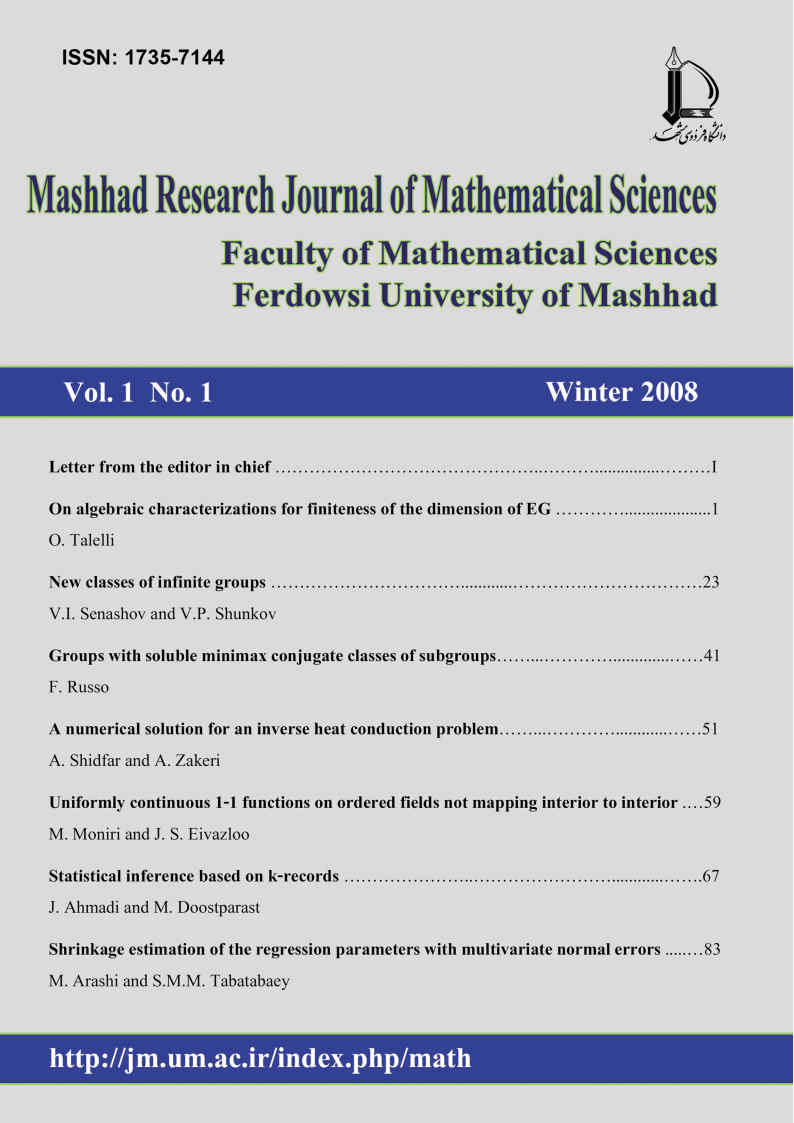
\includegraphics[keepaspectratio]{images/img_013.jpg}}

}

\caption{image}

\end{figure}%

\begin{figure}[H]

{\centering \pandocbounded{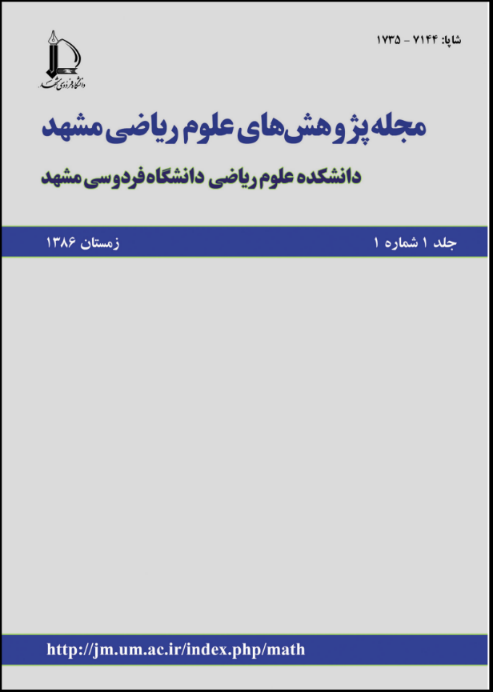
\includegraphics[keepaspectratio]{images/img_027.png}}

}

\caption{image}

\end{figure}%

Mashhad Research Journal of Mathematical Sciences

Editor in Charge

H.R. Tareghian

Editor in Chief

M.R.R. Moghaddam

Managing Editor

H. Jabbari Nooghabi

در سال ۱۳۸۹ و در پی سیاست‌های جدید معاونت پژوهشی وزارت علوم، تحقیقات و
فناوری مبنی بر تخصصی‌تر شدن مجلات دانشگاهی، دانشکده علوم ریاضی ناگزیر از
تغییر و تحدید قلمرو فعالیت مجله مزبور گردید. این امر منجر به تغییر عنوان
مجله، ترکیب هیأت تحریریه و سردبیر شد. «مجله ایرانی آنالیز عددی و
بهینه‌سازی» توسط گروه ریاضی کاربردی دانشکده علوم ریاضی با هدف گسترش دانش
ریاضی در زمینه‌های آنالیز عددی و بهینه‌سازی، و نیز تعامل ملی و بین‌المللی
با ریاضیدانان داخل و خارج از کشور راه‌اندازی شد.

\begin{figure}[H]

{\centering \pandocbounded{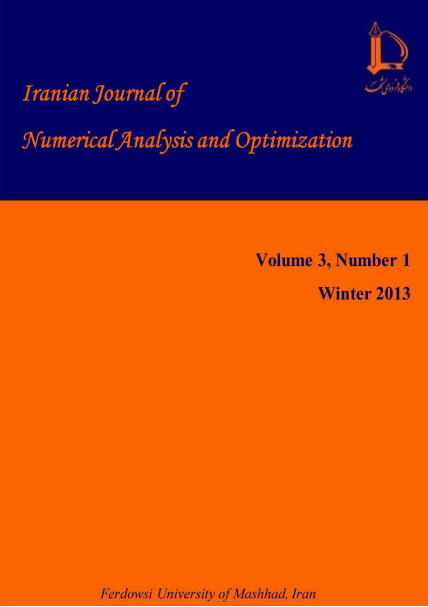
\includegraphics[keepaspectratio]{images/img_090.png}}

}

\caption{image}

\end{figure}%

این مجله از تاریخ ۲۵ دی ۱۳۹۲ به عنوان نشریه‌ای علمی-پژوهشی مورد تأیید
وزارت متبوع به کار خود ادامه داده و موفق به کسب رتبه دوم نشریات دانشگاه
فردوسی مشهد شده است (این امتیاز در سامانه ارزیابی نشریات علمی کشور قابل
تأیید است). شایان ذکر است که این مجله در سال ۲۰۱۵ موفق به کسب امتیاز
۳‎EJCR از پایگاه ISC نیز گردید. در ادامه، در اردیبهشت ۱۳۹۹ برای نمایه‌سازی
در Scopus پذیرفته شد و در سال ۲۰۲۱ موفق به کسب رتبه چارک چهارم (Q۴) در
این پایگاه معتبر گردید.

Editor in Charge

H. R. Tareghian

Editor in Chief

M. H. Farahi

Managing Editor

M. Gachpazan

مجله در سال‌های ۲۰۱۳ تا ۲۰۲۱ به صورت دوماهنامه منتشر می‌شد. جلد ۱۲، شماره
۳، سال ۲۰۲۲، با اختصاص ویژه‌نامه‌ای به مناسبت هفتاد و پنجمین سالگرد تولد
پروفسور آ. وحیدیان و پروفسور ف. توتونیان انتشار یافت.

\begin{figure}[H]

{\centering \pandocbounded{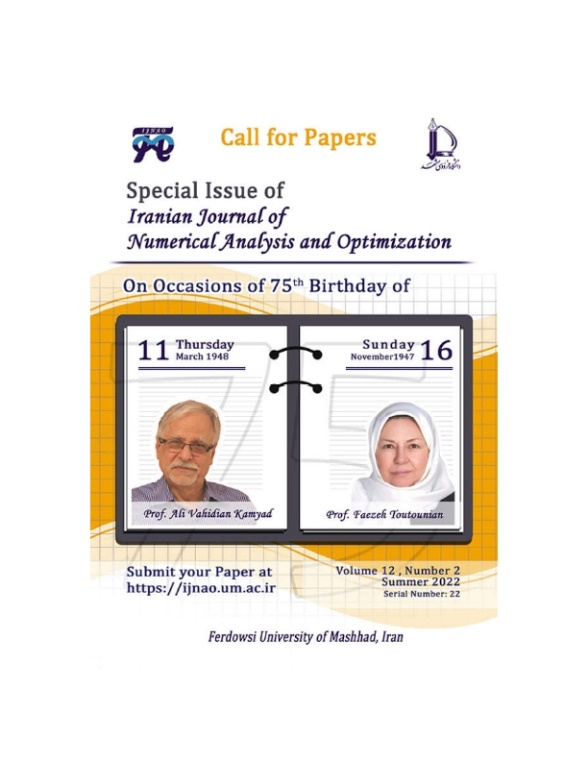
\includegraphics[keepaspectratio]{images/img_101.jpeg}}

}

\caption{image}

\end{figure}%

از سال ۲۰۲۳، مجله به صورت فصلنامه و با ۶۰ مقاله در هر سال به چاپ می‌رسد.
اکنون هیأت تحریریه مجله متشکل از ۳۷ عضو است که ۷ نفر از آنان از اعضای
هیأت علمی دانشکده علوم ریاضی دانشگاه فردوسی مشهد و ۲۷ نفر دیگر از
دانشگاه‌های داخل و خارج از کشور هستند. در سال ۲۰۲۵، این مجله موفق به
ارتقا به چارک سوم (Q۳) در پایگاه Scopus شد. همچنین قطب علمی مدل‌سازی و
کنترل دستگاه‌ها در دانشکده، از حامیان این مجله محسوب می‌شود.

این نشریه در پایگاه‌های اطلاعاتی زیر نمایه می‌شود

نسخه الکترونیکی مقالات در وب‌سایت نشریه به آدرس زیر قابل دسترسی است و
سایر اطلاعات مجله نیز در این سایت قابل مشاهده می‌باشد:

https://ijnao.um.ac.ir

اعضای هیأت تحریریه مجله در سال‌های (۲۰۲۳-۲۰۲۶)

Director-in-Charge

\begin{figure}[H]

{\centering \pandocbounded{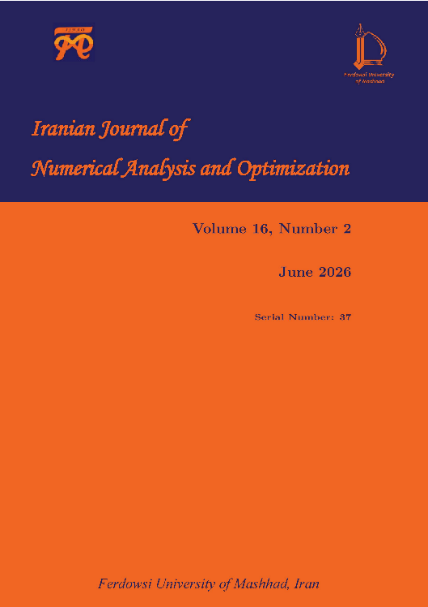
\includegraphics[keepaspectratio]{images/img_108.png}}

}

\caption{image}

\end{figure}%

Farahi, M. H. (Iran)

Editor-in-Chief

Soheili, Ali R. (Iran)

Managing Editor

Gachpazan, M. (Iran)

Language Editor:

Zohreh Vasagh

\section{مجله ریاضی
خیام}\label{ux645ux62cux644ux647-ux631ux6ccux627ux636ux6cc-ux62eux6ccux627ux645}

\section{Khayyam Journal of Mathematics
(KJM)}\label{khayyam-journal-of-mathematics-kjm}

مجله بین‌المللی ریاضی خیام با دسترسی‌آزاد، داوری‌شده و کاملاً الکترونیکی است
که از سال ۲۰۱۵ به انتشار مقالات پژوهشی بدیع و باکیفیت به زبان انگلیسی
می‌پردازد. این مجله از ابتدای انتشار تا پایان سال ۲۰۲۵، با همکاری گروه
پژوهشی ریاضی طوسی و قطب علمی آنالیز روی ساختارهای جبری و گروه ریاضی محض
دانشکده علوم ریاضی دانشگاه فردوسی مشهد، فعالیت می‌کرد و از سال ۲۰۲۶،
دانشگاه فردوسی مشهد به‌عنوان ناشر اصلی، مسئولیت انتشار آن را بر عهده
گرفته است.

حوزه‌های موضوعی این مجله گسترده است و شامل آنالیز ریاضی، جبر (از جمله جبر
جابجایی، جبر همولوژی و جبر خطی و چندخطی)، ترکیبیات، ترکیبیات جبری، نظریه
گروه‌ها، گروه‌های توپولوژیک، هندسه، توپولوژی (شامل توپولوژی عمومی و جبری)،
معادلات دیفرانسیل (معمولی و با مشتقات جزئی)، سیستم‌های دینامیکی، آنالیز
هارمونیک انتزاعی، آنالیز تابعی و نظریه عملگرها می‌شود. مقالات این مجله با
تأکید بر نتایج عمیق، ایده‌های نوین و تأثیرگذاری علمی قابل‌توجه، در قالب
مقالات تحقیقاتی اصیل و گاه مقالات مروری به چاپ می‌رسند.

مجله خیام از نمایه‌های معتبر بین‌المللی چون Scopus، MathSciNet، DOAJ و
Zentralblatt MATH بهره می‌برد. بر اساس تازه‌ترین رتبه‌بندی SCImago Journal
Rank -- SJR در سال ۲۰۲۴، این مجله با امتیاز ۰.۲۲۳ در رده چهارم (Q۴) از
میان نشریات حوزه ریاضیات قرار دارد. شایان ذکر است که رتبه کیفی (Q-Rank)
این مجله از سال ۲۰۱۹ تاکنون نوساناتی داشته و در سال‌های ۲۰۲۰، ۲۰۲۲، ۲۰۲۳
و ۲۰۲۴ در رده Q۴ قرار گرفته است.

نسخه الکترونیکی تمامی مقالات این مجله به‌صورت رایگان و بدون هزینه برای
نویسندگان و خوانندگان، روی وب‌سایت رسمی نشریه به نشانی
https://kjm.um.ac.ir/ در دسترس است و علاقه‌مندان می‌توانند برای کسب
اطلاعات جامع درباره ضوابط انتشار، دوره‌های پیشین و آخرین اخبار، به این
پایگاه اطلاعاتی مراجعه کنند. همچنین، این مجله از سال ۲۰۲۴، مدل انتشار
مقاله‌ای پیوسته (CAP) را به کار گرفته است که طی آن مقالات پذیرفته‌شده
بلافاصله پس از طی فرایند تولید، به‌صورت نهایی در یک شماره منتشر می‌شوند و
این رویه، زمان کلی انتشار را به‌طور چشمگیری کاهش داده است.

اعضای هیأت تحریریه مجله از ابتدا تاکنون

Director-in-Charge:

\begin{figure}[H]

{\centering \pandocbounded{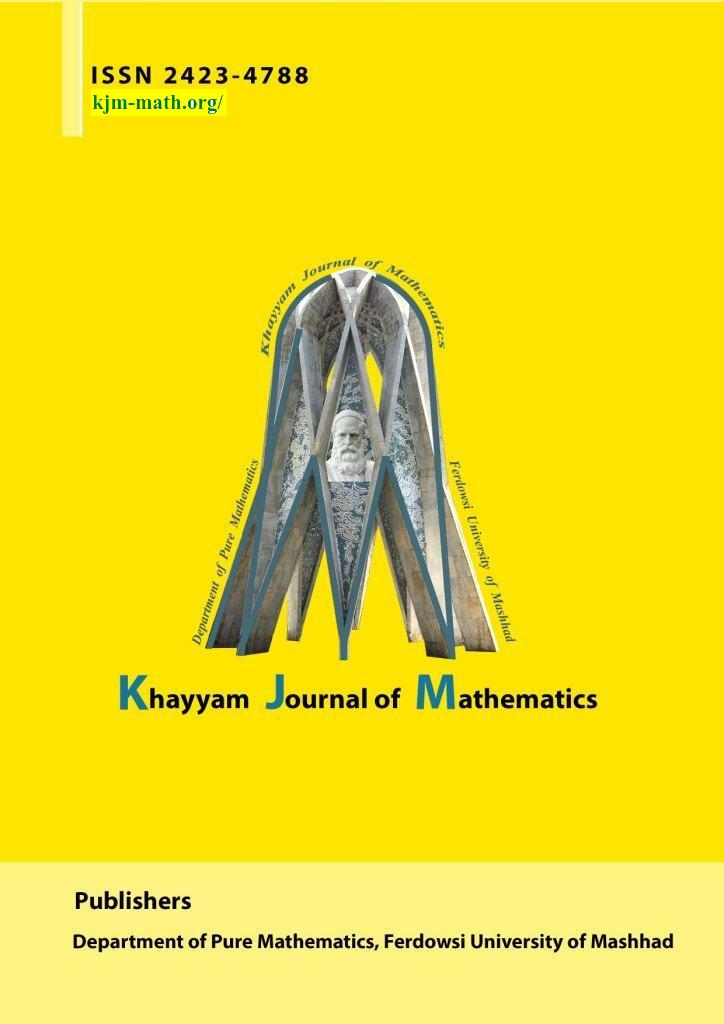
\includegraphics[keepaspectratio]{images/img_044.jpg}}

}

\caption{image}

\end{figure}%

Sal Moslehian, Mohammad (۲۰۱۵-۲۰۲۶)

Editor-in-Chief:

Ebrahimi Vishki, Hamid Reza (۲۰۱۵-۲۰۲۶)

Mashayekhy, Behrooz (۲۰۱۵-۲۰۲۰)

Managing Editor:

Hejazian, Shirin (۲۰۱۵-۲۰۲۳)

Mashayekhy, Behrooz (۲۰۲۳-۲۰۲۶)

Sections Editors:

Ghane, Fatemeh Helen (۲۰۲۰-۲۰۲۶)

Mashayekhy, Behrooz (۲۰۲۰-۲۰۲۳)

Hejazian, Shirin (۲۰۲۳-۲۰۲۶)

Kamel Mirmostafaee, Alireza (۲۰۲۰-۲۰۲۶)

Language Editor:

Erfanian, Ahmad (۲۰۱۵-۲۰۲۰)

Mirzavaziri, Madjid (۲۰۱۵-۲۰۲۰)

Vasagh, Zohreh (۲۰۲۰-۲۰۲۶)

Technical Editor:

Kamyabi-Gol, Rajab Ali (۲۰۱۵-۲۰۲۰)

\section{مجله مدل‌های تصادفی در احتمال و
آمار}\label{ux645ux62cux644ux647-ux645ux62fux644ux647ux627ux6cc-ux62aux635ux627ux62fux641ux6cc-ux62fux631-ux627ux62dux62aux645ux627ux644-ux648-ux622ux645ux627ux631}

\section{Stochastic Models in Probability and Statistics
(SMPS)}\label{stochastic-models-in-probability-and-statistics-smps}

از سال ۲۰۲۴ مجله SMPS با هدف انتشار مقالات علمی-پژوهشی به زبان انگلیسی
درحوزه‌های مدل‌های تصادفی در احتمال و آمار شروع به کار کرده است. محورهای
پژوهشی آن با تأکید بر کاربردهای مدل های آمار و احتمال در مسائل قابلیت
اطمینان است. SMPS مقالات در موضوعات روش‌های ریاضی در قابلیت اطمینان،
تحلیل داده‌های طول عمر، مدل‌های بیری و افزایش طول عمر، مدل‌سازی آماری در
قابلیت اطمینان، روش‌های آماری در تحقیقات عملیاتی، مدل‌های تصادفی در مهندسی
صنایع و سیستم‌ها، مدل‌سازی بهینه در نگهداری و تعمیرات، کنترل کیفیت و
فرآیند نظارت، روش‌های ناپارامتری در تحلیل طول عمر، روش‌های آماری در نظریه
اطلاعات، مدل‌های داده‌های ترتیبی و کاربردهای آنها، ترتیب های تصادفی،
قابلیت اطمینان نرم‌افزار، تحلیل داده‌ها در قابلیت اطمینان، روش‌های مفصل و
مدل‌سازی وابستگی، کلان داده و کاربردهای قابلیت اطمینان منتشر می‌کند.

اعضای هیأت تحریریه مجله

Director-in-Charge

\begin{figure}[H]

{\centering \pandocbounded{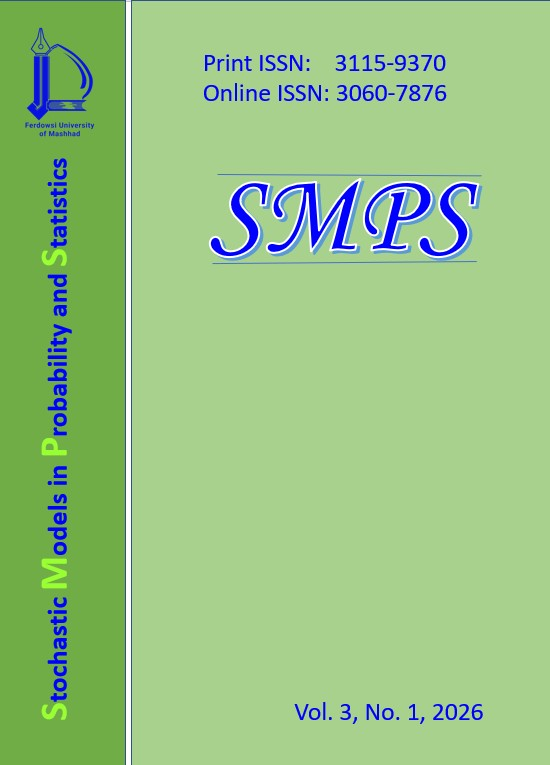
\includegraphics[keepaspectratio]{images/img_062.png}}

}

\caption{image}

\end{figure}%

Jafar Ahmadi (Iran)

Editor-in-Chief

Jafar Ahmadi (Iran)

Executive Editor

Mahdi Doostparast (Iran)

Managing Editor

Mostafa Razmkhah (Iran)

Technical Editor

Hadi Jabbari Nooghabi (Iran)

English Text Editor

Zohreh Vasagh (Iran)

\section{مجله به سوی علوم
ریاضی}\label{ux645ux62cux644ux647-ux628ux647-ux633ux648ux6cc-ux639ux644ux648ux645-ux631ux6ccux627ux636ux6cc}

\section{Toward Mathematical
Sciences}\label{toward-mathematical-sciences}

این نشریه علمی-ترویجی از سال ۱۴۰۰ به انتشار مقالات فارسی پرداخته است.
مجله به سوی علوم ریاضی مقالات در زمینه‌های ریاضی محض، ریاضی کاربردی، آمار
و احتمال، علوم کامپیوتر، آموزش ریاضی، تاریخ و فلسفه ریاضی، کاربردهای
ریاضی، آمار و علوم کامپیوتر در سایر علوم، و نقدهای علمی را برای بررسی می
پذیرد. همچنین ترجمه مقالاتی در موضوعات گفته شده نیز با شرایط خاص مورد
بررسی قرار می گیرد.

مدیر مسئول

\begin{figure}[H]

{\centering \pandocbounded{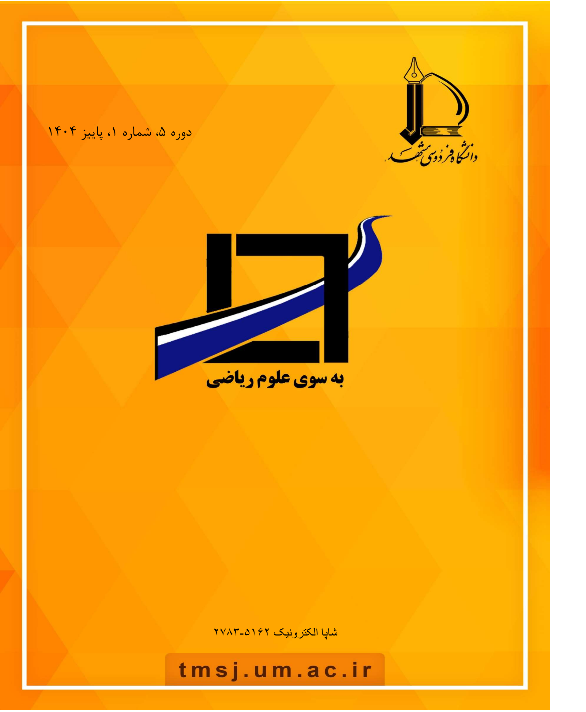
\includegraphics[keepaspectratio]{images/img_079.png}}

}

\caption{image}

\end{figure}%

محمد صال مصلحیان

سردبیر

بهروز مشایخی فرد

مدیر اجرایی

محمد جانفدا

ویراستار

زهره وثاق

\bookmarksetup{startatroot}

\chapter{بخش
رایانه}\label{ux628ux62eux634-ux631ux627ux6ccux627ux646ux647}

\bookmarksetup{startatroot}

\chapter{بخش
رایانه}\label{ux628ux62eux634-ux631ux627ux6ccux627ux646ux647-1}

دانشکده علوم ریاضی دارای یک شبکه رایانه مجهز به تعداد بیش از ۲۰۰
کامپیوتر است که امکان استفاده از اینترنت برای اعضای هیأت علمی و کارکنان
و دانشجویان فراهم شده است. اعضای هیأت علمی و اتاق کار دانشجویان دکتری و
اتاق کارکنان دارای رایانه شخصی و چاپگر میباشد.

شبکه دانشکده

سیستم شبکه این دانشکده بصورت ستاره‌ای میباید و از سوئیچ های سیسکو برای
امنیت بالاتر استفاده شده است.

سایت رایانه دانشجویان کارشناسی

این بخش مشتمل بر ۲۸ دستگاه رایانه برای اجرای برنامه‌های سبک و متوسط با
نرم‌افزارهای مختلف آمار و ریاضی (Matlab، Maple، Spss، Mathematica و R) و
برنامه‌نویسی و امور تایپ با استفاده از نرم‌افزار XePersian و استفاده از
اینترنت پرسرعت دانشگاه برای دانشجویان دوره کارشناسی است و همه روزه از
ساعت ۷ صبح الی ۱۸ عصر آماده ارائه خدمات نرم‌افزاری به دانشجویان دوره
کارشناسی در دانشکده است.

کارگاه آموزشی

دانشکده شامل سه کارگاه آموزشی میباشد:

کارگاه آموزشی شماره ۱ : با ۲۸ دستگاه رایانه مخصوص و پرسرعت در خدمت آموزش
نرم‌افزارهای کاربردی به دانشجویان در کلاس‌های دروس کاربردی دانشکده است.

کارگاه آموزشی شماره ۲ : با ۲۵ دستگاه رایانه مخصوص و پرسرعت در خدمت آموزش
نرم‌افزارهای کاربردی به دانشجویان در کلاس‌های دروس کاربردی دانشکده است.

کارگاه آموزشی شماره ۳ : با ۱۷ دستگاه رایانه مخصوص و پرسرعت در خدمت آموزش
نرم‌افزارهای کاربردی به دانشجویان در کلاس‌های دروس کاربردی دانشکده است.

سایت رایانه دانشجویان تحصیلات تکمیلی (دانشجویان دکتری و کارشناسی ارشد)

آزمایشگاه رایانه دانشکده علوم ریاضی با ارائه خدمات مستمر و پاسخگویی
نیازهای دانشجویان تحصیلات تکمیلی در امور رایانه است. این بخش مشتمل بر ۳۲
دستگاه رایانه برای اجرای برنامه‌های سبک و متوسط با نرم‌افزارهای مختلف آمار
و ریاضی (Matlab، Maple، Spss، Mathematica و R) و امور تایپ با استفاده از
نرم‌افزار XePersian و استفاده از اینترنت پرسرعت دانشگاه برای دانشجویان
تحصیلات تکمیلی است و همه روزه از ساعت ۷ صبح الی ۱۸ عصر آماده ارائه خدمات
نرم‌افزاری به دانشجویان تحصیلات تکمیلی در دانشکده است.

آزمایشگاه محاسبات سنگین

در سال‌های ۹۴ تا ۹۵ نیز تعداد ۶ دستگاه کامپیوتر محاسباتی با قدرت پردازش
بالا برای انجام محاسبات سنگین با نرم‌افزارهای آمار و به این مجموعه اضافه
شده است.

کلاس ها

دانشکده شامل ۱۵ عدد کلاس میباشد که کلیه کلاس ها مجهز به سیستم پرسرعت و
پرژکتور می باشد.

سمینارها

دانشکده شامل ۵ عدد سمینار جهت برگزاری جلسات و دفاع دانشجویان تحصیلات
تکمیلی میباشد که کلیه سمینار ها مجهز به سیستم پرسرعت و پرژکتور می باشد.

\bookmarksetup{startatroot}

\chapter{آزمایشگاه‌ها}\label{ux622ux632ux645ux627ux6ccux634ux6afux627ux647ux647ux627}

\bookmarksetup{startatroot}

\chapter{آزمایشگاههای
دانشکده}\label{ux622ux632ux645ux627ux6ccux634ux6afux627ux647ux647ux627ux6cc-ux62fux627ux646ux634ux6a9ux62fux647}

\section{آزمایشگاه
بازی‌سازی}\label{ux622ux632ux645ux627ux6ccux634ux6afux627ux647-ux628ux627ux632ux6ccux633ux627ux632ux6cc}

آزمایشگاه فناوری بازی‌سازی دانشکده علوم ریاضی در شهریورماه ۱۳۹۷ به همت
دکتر رسول رمضانیان فعالیت خود را آغاز کرد. در دی‌ماه همان سال، ریاست
بنیاد ملی بازی‌های رایانه‌ای از عملکرد آزمایشگاه بازدید به عمل آورد؛
بازدیدی که نشان‌دهنده جایگاه رو به رشد این آزمایشگاه در سطح ملی بود. از
آن زمان تاکنون، دانشجویان این آزمایشگاه چندین بازی در حوزه بازی‌های
رایانه‌ای کودکان طراحی و تولید کرده‌اند که در همایش‌های رسمی به نمایش
گذاشته شده‌اند.

اهداف اصلی این آزمایشگاه عبارت‌اند از:

آماده‌سازی دانشجویان برای ورود و فعالیت در صنعت بازی‌سازی

انجام تحقیقات در حوزه بازی‌انگاری (Gamification) و راهکارهای کاربست آن

به‌کارگیری فرایندهای بازی‌محور در حوزه علوم انسانی

این آزمایشگاه به رایانه‌های مخصوص محاسبات سنگین مجهز است که بر روی آن‌ها
نرم‌افزارها و ابزارهای تخصصی زیر نصب و راه‌اندازی شده‌اند:

Unity۳D

Node.js

Photoshop

After Effects

در خردادماه سال ۱۴۰۱ این ازمایشگاه به بلاکچین تغییر نام داد و لازم به
ذکر است که فعالیت این آزمایشگاه، به دلیل عدم حضور مدیر مسئول آن و سپری
کردن فرصت مطالعاتی ایشان، مدتی است متوقف شده و در انتظار از سرگیری مجدد
است.

\section{آزمایشگاه
بهینه‌سازی}\label{ux622ux632ux645ux627ux6ccux634ux6afux627ux647-ux628ux647ux6ccux646ux647ux633ux627ux632ux6cc}

امروزه علم بهینه‌سازی به‌عنوان یکی از ابزارهای کلیدی در مدل‌سازی، تحلیل
داده‌ها و ارتقای کیفی نتایج عملی در حوزه‌های گوناگون علمی شناخته می‌شود. از
مهندسی و مدیریت گرفته تا کشاورزی و علوم کامپیوتر، همه به دنبال یافتن
بهترین پاسخ ممکن در میان انبوهی از گزینه‌ها هستند. در همین راستا،
آزمایشگاه بهینه‌سازی دانشگاه فردوسی مشهد در سال ۱۳۹۶ با همت دکتر رضا
قنبری، عضو هیأت علمی گروه ریاضی کاربردی، تأسیس شد تا پاسخی نظام‌مند به
این نیاز روزافزون باشد.

\begin{figure}[H]

{\centering \pandocbounded{
\includegraphics[keepaspectratio]{images/img_008.jpeg}}

}

\caption{image}

\end{figure}%

هدف اصلی این آزمایشگاه، ایجاد پلی میان ریاضیات محض و کاربردهای واقعی آن
است. در این مرکز، پژوهشگران با مدل‌سازی دقیق مسائل، حل مؤثر مدل‌ها و تحلیل
حساسیت نتایج، بستری فراهم می‌آورند تا رشته‌های مختلف علمی و حتی شرکت‌ها و
دستگاه‌های اجرایی بتوانند از ظرفیت‌های بهینه‌سازی بهره ببرند. ماهیت
نرم‌افزاری آزمایشگاه نیز امکان تولید بسته‌های نرم‌افزاری تجاری و همچنین
ابزارهای متن‌باز تحقیقاتی را فراهم کرده است.

یکی از سیاست‌های کلیدی آزمایشگاه، حمایت از جامعه علمی دانشگاه فردوسی است.
به‌گونه‌ای که خدمات آن برای مخاطبان غیر علوم ریاضی با دریافت هزینه ارائه
می‌شود، اما در بیشتر موارد، اعضای علوم ریاضی دانشگاه می‌توانند بدون هزینه
از خدمات مشاوره‌ای، پیاده‌سازی مدل در نرم‌افزارهای تجاری، تحلیل مدل‌ها،
طراحی الگوریتم‌های بهینه‌سازی و هوشمند، و حتی طراحی مدل‌های تجاری بهره‌مند
شوند.

با توجه به نوپا بودن چنین آزمایشگاه‌هایی در کشور، دو چشم‌انداز برای آینده
آن ترسیم شده است: در میان‌مدت، آزمایشگاه با تولید کدهای نرم‌افزاری و
مدل‌سازی‌های گوناگون، نیازهای پژوهشی دانشجویان و اساتید رشته‌های مرتبط را
در سطح دانشگاه پاسخ می‌دهد و همزمان، به دانشجویان شاغل در آزمایشگاه،
تجربه ارزشمند عملی در محاسبات می‌آموزد. در درازمدت، با تجمیع تخصص‌های
گوناگون، این مرکز به دروازه ارتباط تخصصی با جامعه منطقه‌ای و ملی تبدیل
خواهد شد و زمینه شکل‌گیری استارتاپ‌هایی برای حل مسائل بهینه‌سازی را فراهم
می‌آورد.

زیرساخت‌های آزمایشگاه شامل یک رایانه قدرتمند برای محاسبات سنگین و چندین
سیستم دیگر برای اجرای پروژه‌های بهینه‌سازی است. تاکنون فعالیت‌های ارزشمندی
در این مرکز انجام شده که از آن جمله می‌توان به پروژه سامانه حمل‌ونقل
هوشمند (VRP)، طراحی سامانه بهره‌وری آب کشاورزی (سیاب) برای استان‌های
خراسان شمالی و خوزستان با دو رویکرد متفاوت بهینه‌سازی ریاضی (در همکاری با
شرکت هیدروتک)، همکاری مشاوره‌ای با دانشگاه‌های سمنان و شریف در زمینه
الگوریتم‌های فراابتکاری، و انجام پژوهش‌های مشترک با دانشکده‌های مهندسی
کامپیوتر، مدیریت و کشاورزی دانشگاه فردوسی اشاره کرد که حاصل آن، ارسال
مقالات متعدد به ژورنال‌های معتبر بوده است. افزون بر این، کلاس‌های آموزشی
برنامه‌نویسی برای دانشجویان مستعد دانشکده برگزار می‌شود تا نسل جدیدی از
متخصصان بهینه‌سازی پرورش یابند.

علاقه‌مندان برای آگاهی از پروژه‌های انجام‌شده و ارتباط با اعضای آزمایشگاه
می‌توانند به وبسایت رسمی آن به آدرس http://optlab.um.ac.ir مراجعه کنند..

\section{آزمایشگاه پردازش زبان
طبیعی}\label{ux622ux632ux645ux627ux6ccux634ux6afux627ux647-ux67eux631ux62fux627ux632ux634-ux632ux628ux627ux646-ux637ux628ux6ccux639ux6cc}

آزمایشگاه پردازش زبان طبیعی در آذرماه سال ۱۴۰۲ در دانشکده علوم ریاضی
دانشگاه فردوسی مشهد تأسیس شد. این آزمایشگاه با هدف توسعه پژوهش‌های علمی و
کاربردی در حوزه تحلیل داده‌های متنی، پردازش زبان طبیعی و مدل‌های زبانی
نوین فعالیت خود را آغاز نمود و در ادامه تجربیات و فعالیت‌های پژوهشی
انجام‌شده در حوزه متن‌کاوی و یادگیری ماشین، به‌ویژه در همکاری‌های پیشین
مرتبط با پژوهشگاه علوم و فناوری اطلاعات ایران (ایرانداک)، شکل گرفت.

\begin{figure}[H]

{\centering \pandocbounded{
\includegraphics[keepaspectratio]{images/img_022.jpeg}}

}

\caption{image}

\end{figure}%

مأموریت اصلی آزمایشگاه، توسعه دانش و کاربردهای پردازش زبان طبیعی و تحلیل
داده‌های متنی در مسائل علمی، صنعتی و سازمانی است. حوزه‌های کلیدی فعالیت آن
شامل مدل‌های زبانی بزرگ و سامانه‌های مولد متن، سامانه‌های پرسش و پاسخ و
تولید مبتنی بر بازیابی اطلاعات (RAG)، متن‌کاوی و استخراج اطلاعات، تحلیل
داده‌های متنی و داده‌کاوی علمی، و همچنین توسعه کاربردهای این فناوری در
حوزه‌های سلامت، آموزش و خدمات سازمانی می‌شود.

مدیریت و راهبری علمی و اجرایی آزمایشگاه از زمان تأسیس تاکنون بر عهده
دکتر جلال‌الدین نصیری، عضو هیأت علمی دانشکده علوم ریاضی، بوده است. دکتر
محمد آرشی نیز به‌عنوان همکار علمی در حوزه‌های پژوهشی و توسعه سامانه‌های
پردازش زبان طبیعی با آزمایشگاه همکاری دارد. افزون بر این، دانشجویان
تحصیلات تکمیلی و پژوهشگران همکار در قالب پروژه‌ها و پایان‌نامه‌های تخصصی در
فعالیت‌های آزمایشگاه مشارکت می‌کنند.

آزمایشگاه از زیرساخت‌های پیشرفته‌ای برای پژوهش، آموزش و توسعه سامانه‌های
مبتنی بر پردازش زبان طبیعی برخوردار است. مهم‌ترین امکانات آن شامل سامانه
مجهز به پردازنده گرافیکی Nvidia RTX ۴۰۹۰ برای آموزش و استقرار مدل‌های
زبانی، بستر اجرای محلی مدل‌های بزرگ با هدف حفظ امنیت اطلاعات، و دسترسی به
ابزارها و چارچوب‌های تخصصی متن‌کاوی و تحلیل داده‌های متنی است.

از زمان تأسیس، آزمایشگاه در اجرای پروژه‌های پژوهشی و کاربردی متعددی
مشارکت داشته است. از جمله پروژه طراحی و توسعه دستیار هوشمند پشتیبانی
سازمانی با همکاری شرکت دانش‌بنیان رایانش ابری فردوسی که به طراحی سامانه
پاسخ‌گویی خودکار مبتنی بر مدل‌های زبانی بزرگ و معماری RAG انجامیده است.
همچنین تفاهم‌نامه همکاری برای توسعه دستیار هوشمند میز خدمت بیمارستان قائم
(عج) در فاز نخست، با هدف پاسخ‌گویی خودکار به پرسش‌های مراجعان و حفظ امنیت
داده‌های درمانی، از دیگر پروژه‌های شاخص به شمار می‌رود. مشارکت در طرح‌های
پژوهشی بنیاد ملی علم ایران (INSF) در حوزه پردازش زبان طبیعی نیز بخشی از
فعالیت‌های این مرکز است.

در کنار پروژه‌های کاربردی، آزمایشگاه به هدایت پایان‌نامه‌ها و پروژه‌های
دانشجویی، توسعه نمونه‌های آزمایشی سامانه‌های گفتگوگر و پاسخ‌گویی مبتنی بر
اسناد، و انتشار مقالات علمی در حوزه داده‌کاوی و پردازش زبان طبیعی پرداخته
است. ارتباطات علمی با پژوهشگران دانشگاه صنعتی شریف و دانشگاه بن آلمان،
گسترش فعالیت‌ها در راستای تحولات مدل‌های زبانی بزرگ، و توسعه زیرساخت‌های
پژوهشی از دیگر اقدامات این آزمایشگاه به شمار می‌رود.

رویکرد اصلی آزمایشگاه، تمرکز بر حل مسائل واقعی و توسعه کاربردهای عملی
پردازش زبان طبیعی در سازمان‌ها و صنایع مختلف است. همکاری با مراکز درمانی،
شرکت‌های فناور و گروه‌های پژوهشی دانشگاهی موجب شده است فعالیت‌های آزمایشگاه
علاوه بر جنبه‌های علمی، در مسیر توسعه راهکارهای کاربردی و پاسخ‌گویی به
نیازهای واقعی جامعه نیز قرار گیرد.

آزمایشگاه پردازش زبان طبیعی در مدت کوتاه فعالیت خود توانسته است به عنوان
یکی از هسته‌های فعال پژوهشی دانشکده علوم ریاضی در حوزه فناوری‌های زبانی و
تحلیل داده‌های متنی شناخته شود و زمینه مناسبی برای انجام پژوهش‌های
میان‌رشته‌ای، تربیت دانشجویان متخصص و توسعه همکاری‌های علمی و صنعتی فراهم
آورد.

\section{آزمایشگاه علم
داده‌ها}\label{ux622ux632ux645ux627ux6ccux634ux6afux627ux647-ux639ux644ux645-ux62fux627ux62fux647ux647ux627}

آزمایشگاه علم داده دانشکده علوم ریاضی دانشگاه فردوسی مشهد (DSLab)
به‌عنوان یکی از نخستین گروه‌های تحقیقاتی میان‌رشته‌ای در حوزه داده‌کاوی و
یادگیری ماشین در شرق کشور، در اردیبهشت‌ماه ۱۴۰۰ فعالیت رسمی خود را آغاز
کرد. ایده تأسیس این آزمایشگاه، ریشه در نیاز روزافزون به تحلیل داده‌های
خام و تبدیل آن‌ها به بینش کاربردی در مسائل واقعی جامعه داشت؛ نیازی که با
گسترش داده‌های کلان در حوزه‌های شهری، صنعتی، اقتصادی و علمی بیش از پیش
احساس می‌شد.

\begin{figure}[H]

{\centering \pandocbounded{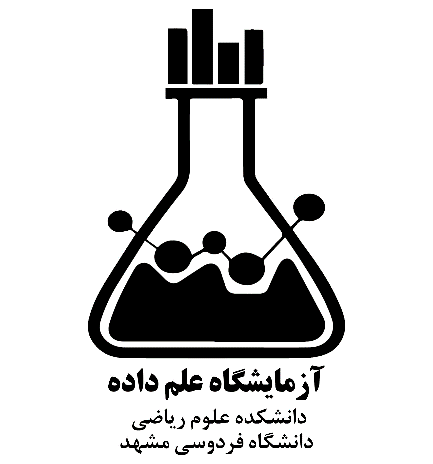
\includegraphics[keepaspectratio]{images/img_036.png}}

}

\caption{image}

\end{figure}%

پیش‌زمینه شکل‌گیری DSLab به سیاست‌های دانشکده علوم ریاضی برای راه‌اندازی
رشته‌های تقاضا‌محور بازمی‌گردد. از همین رو، دانشکده با هدف پرورش نیروی
انسانی متخصص در علم داده و ایجاد پل ارتباطی میان دانشگاه و نهادهای
اجرایی، اقدام به تأسیس این آزمایشگاه کرد. گروه هدف اولیه، دانشجویان و
پژوهشگرانی بودند که در زمینه‌های آمار، ریاضیات کاربردی و علوم کامپیوتر به
مدل‌سازی پدیده‌های دارای عدم‌قطعیت علاقه داشتند.

مراسم افتتاحیه آزمایشگاه در روز دوشنبه ۲۱ اردیبهشت‌ماه ۱۴۰۰، همزمان با
هفته سرآمدی آموزش، به‌صورت ترکیبی (حضوری و مجازی) برگزار شد. در این
رویداد، دکتر سهیلی، رئیس وقت دانشکده، از راه‌اندازی رشته علم داده در مقطع
کارشناسی ارشد خبر داد و بر مشارکت DSLab با رصدخانه شهری شهرداری مشهد
تأکید کرد. سپس دکتر محمد آرشی، مسئول راه‌اندازی آزمایشگاه، اهداف کلان را
شامل حل مسائل واقعی جامعه، توسعه ابزارهای محاسباتی مبتنی بر روش‌های
آماری، تهیه پایگاه‌های داده تخصصی، تربیت نیروی متخصص، و اجرای پروژه‌های
اجتماعی، صنعتی و اقتصادی برشمرد. در ادامه، از وبسایت رسمی آزمایشگاه به
آدرس http://dslab.um.ac.ir رونمایی شد.

در بخش علمی مراسم، دکتر مظلوم، پژوهشگر پسادکتری علم داده از دانشگاه
آمستردام، به بیان چگونگی شکل‌گیری علم داده در سال ۲۰۱۳ بر اثر سه انفجار
بزرگ در تولید داده‌های کلان، سخت‌افزار و یادگیری عمیق پرداخت و بر لزوم
ارتباط آزمایشگاه با صنایع خودروسازی، نفت، فولاد و نهادهایی مانند شهرداری
و پلیس تأکید کرد. افتتاحیه با حضور هیأت رئیسه، جمعی از اساتید و مدیرانی
از شهرداری مشهد و مرکز نوآوری شهری به پایان رسید.

ساختار آزمایشگاه از ابتدا به‌گونه‌ای طراحی شد که هم از ظرفیت علمی اعضای
هیأت علمی (در گروه‌های آمار، ریاضی کاربردی و علوم کامپیوتر) و هم از توان
دانشجویان علاقه‌مند بهره گیرد. شورای راهبری اصلی با حضور اساتید و محققان
بین‌المللی و شورای راهبری دانشجویی برای برنامه‌ریزی فعالیت‌ها، وبسایت و
رسانه‌های اجتماعی تشکیل گردید. همچنین همکاران غیرمقیم از دانشگاه‌های
تهران، یزد و نیشابور و مشاورانی از کانادا و پرتغال، اعتبار علمی
آزمایشگاه را افزایش دادند.

از ابتدای تأسیس، DSLab با برگزاری کارگاه‌ها، سخنرانی‌های تخصصی و جلسات
منظم علمی، فعالیت خود را آغاز کرد. وبسایت دوزبانه (فارسی-انگلیسی)، حضور
در شبکه لینکداین و بخش درخواست همکاری، از اقدامات اولیه برای
بین‌المللی‌سازی و جذب نیرو بود. همچنین در ارزیابی اولیه نسبت به همتایان
داخلی (مانند آزمایشگاه‌های دانشگاه تهران، شریف و صنعتی امیرکبیر) و خارجی
(همچون MIT، EPFL و دانشگاه کپنهاگ)، نقاط قوتی مانند شورای دانشجویی،
شفافیت برنامه‌ها و همکاری چندرشته‌ای شناسایی شد.

با گذشت زمان، پیشنهادهایی برای بهبود گرافیک وبسایت، نمایش دستاوردها،
ایجاد بخش‌های خدماتی، همکاری با گروه‌های علوم انسانی و مهندسی، برگزاری
کارگاه‌های آشنایی با داده‌کاوی در مدارس، و تقویت ارتباط با صنعت مطرح
گردید. هدف نهایی، تبدیل DSLab به مرکزی پیشرو در تحلیل داده و حل مسائل
کلان‌شهری و صنعتی با رویکردی علمی، آموزشی و کاربردی است. امروزه این
آزمایشگاه به‌عنوان یکی از قطب‌های نوپای علم داده در کشور، مسیر رشد و گسترش
همکاری‌های ملی و بین‌المللی را دنبال می‌کند.

\section{آزمایشگاه قابلیت اعتماد
محاسباتی}\label{ux622ux632ux645ux627ux6ccux634ux6afux627ux647-ux642ux627ux628ux644ux6ccux62a-ux627ux639ux62aux645ux627ux62f-ux645ux62dux627ux633ux628ux627ux62aux6cc}

در دنیای صنعتی امروز، اعتماد مشتریان به محصولات و کیفیت خدمات پس از
فروش، یکی از ارکان اصلی موفقیت و بقا در بازارهای رقابتی به شمار می‌رود.
صنایع پیشرو همواره به دنبال روش‌هایی علمی برای افزایش بهره‌وری، کاهش
هزینه‌ها و بهبود فرآیندهای تولیدی خود هستند. در این میان، تحلیل عددی
قابلیت اعتماد سیستم‌ها و تهیه برنامه‌های بهینه نگهداری و تعمیرات، نقشی
کلیدی ایفا می‌کند. بر این اساس، آزمایشگاه قابلیت اعتماد محاسباتی در
پانزدهم آبان‌ماه سال ۱۴۰۳ در دانشکده علوم ریاضی دانشگاه فردوسی مشهد تأسیس
شد تا پاسخی علمی و عملی به این نیاز اساسی صنایع کشور باشد.

\begin{figure}[H]

{\centering \pandocbounded{
\includegraphics[keepaspectratio]{images/img_056.png}}

}

\caption{image}

\end{figure}%

مأموریت اصلی این آزمایشگاه، بر خلاف بسیاری از مراکز دانشگاهی که بر آموزش
و پژوهش متمرکز هستند، به‌طور ویژه بر اجرای طرح‌های برون‌دانشگاهی و ارائه
خدمات تخصصی به صنایع و سازمان‌های دولتی و غیردولتی متمرکز است. در واقع،
آزمایشگاه قابلیت اعتماد محاسباتی با هدف پر کردن شکاف میان دانش نظری و
نیازهای عینی صنعت پا به عرصه وجود نهاد و تلاش می‌کند تا با بهره‌گیری از
روش‌های نوین آماری و تحلیل داده‌های طول عمر و فرسودگی، به افزایش کیفیت و
کاهش ریسک‌های تولیدی کمک نماید.

حوزه‌های فعالیت این آزمایشگاه طیف گسترده‌ای از خدمات تخصصی را در بر
می‌گیرد: ارزیابی عددی قابلیت اعتماد سیستم‌های مهندسی در صنایع گوناگون،
تحلیل داده‌های طول عمر و فرسودگی با استفاده از روش‌های آماری پیشرفته،
برنامه‌ریزی نگهداری و تعمیرات مبتنی بر شاخص‌های قابلیت اعتماد، و ارائه
مشاوره به مجریان طرح‌های برون‌دانشگاهی. افزون بر این، اجرای مستقیم طرح‌های
کاربردی در همکاری با صنایع خودروسازی، نفت، فولاد و سایر بخش‌های تولیدی و
خدماتی، از دیگر اهداف کلیدی این مرکز به شمار می‌رود.

مدیریت علمی و اجرایی آزمایشگاه از زمان تأسیس تاکنون بر عهده دکتر مهدی
دوست‌پرست، استاد برجسته گروه آمار دانشگاه فردوسی مشهد، بوده است. ایشان با
بهره‌گیری از تجربیات ارزشمند خود در حوزه قابلیت اعتماد و آمار صنعتی، مسیر
رشد و توسعه این مرکز را هدایت می‌کنند. در کنار ایشان، جمعی از اساتید
برجسته و پژوهشگران مطرح کشور، از جمله دکتر جعفر احمدی، دکتر عبدالحمید
رضائی‌رکن‌آبادی، دکتر مجید اسدی از دانشگاه اصفهان، دکتر محمد خنجری صادق،
دکتر مصطفی رزمخواه، دکتر آرزو حبیبی‌راد و دکتر فرهاد کلاهان، به‌عنوان
اعضای اصلی و همکاران علمی، آزمایشگاه را در دستیابی به اهداف خود یاری
می‌رسانند. این ترکیب ارزشمند از تخصص‌های گوناگون در حوزه آمار و قابلیت
اعتماد، بستری مناسب برای انجام پروژه‌های پیچیده و کاربردی فراهم آورده
است.

آزمایشگاه قابلیت اعتماد محاسباتی با رویکردی مسئله‌محور و نتیجه‌گرا، در نظر
دارد تا با ارائه خدمات مشاوره‌ای و اجرایی به صنایع مختلف، به مرجعی معتبر
در حوزه ارزیابی قابلیت اعتماد و نگهداری و تعمیرات در کشور تبدیل شود. با
توجه به ساختار مأموریت‌گرای این مرکز و بهره‌مندی از توان علمی اساتید مجرب،
انتظار می‌رود که در مدت کوتاهی، گام‌های مؤثری در جهت افزایش بهره‌وری، کاهش
هزینه‌های تولید و بهبود کیفیت محصولات صنایع کشور برداشته شود و زمینه برای
ارتباط هرچه بیشتر دانشگاه با جامعه و صنعت فراهم آید.

\section{آزمایشگاه کنترل و هوش
مصنوعی}\label{ux622ux632ux645ux627ux6ccux634ux6afux627ux647-ux6a9ux646ux62aux631ux644-ux648-ux647ux648ux634-ux645ux635ux646ux648ux639ux6cc}

آزمایشگاه کنترل و هوش مصنوعی (CAILab) در دانشکده علوم ریاضی دانشگاه
فردوسی مشهد با مسئولیت دکتر سهراب عفتی در آذر ماه سال ۱۴۰۲، با هدف پیوند
دادن مباحث نظری کنترل با رویکردهای نوین هوش مصنوعی شکل گرفت. در ابتدا،
تمرکز اصلی این آزمایشگاه بر مباحث پایه‌ای کنترل تطبیقی و سیستم‌های
دینامیکی بود، اما با گذر زمان و تجهیز تدریجی به رایانه‌های قدرتمند و
ابزارهای تحقیقاتی تخصصی، دامنه فعالیت آن به سوی حوزه‌هایی نوین‌تر همچون
یادگیری ماشین، شبکه‌های عصبی و مدل‌سازی هوش مصنوعی گسترش یافت.

این تحول تدریجی، آزمایشگاه را به جایگاهی رساند که بتواند پژوهش‌های خود را
از فضای صرفاً نظری به سوی کاربردهای صنعتی واقعی هدایت کند. از جمله این
مسیرها، همکاری در تحلیل و بهینه‌سازی سیستم‌های کنترلی در حوزه‌هایی متنوع
چون پزشکی، صنایع معدنی (نمونه آن همکاری با معدن گل‌گهر سیرجان) و صنایع
انرژی بوده است؛ پروژه‌هایی که نشان‌دهنده گسترش تعامل آزمایشگاه با صنایع
مختلف کشور در طول سال‌های فعالیت آن است.

\section{آزمایشگاه نظریه گراف و کاربردهای
آن}\label{ux622ux632ux645ux627ux6ccux634ux6afux627ux647-ux646ux638ux631ux6ccux647-ux6afux631ux627ux641-ux648-ux6a9ux627ux631ux628ux631ux62fux647ux627ux6cc-ux622ux646}

آزمایشگاه نظریه گراف و کاربردهای آن، به‌عنوان یکی از آزمایشگاه‌های تخصصی
دانشکده علوم ریاضی دانشگاه فردوسی مشهد، با هدفی روشن پا به عرصه وجود
نهاد: پیوند دادن مفاهیم عمیق و انتزاعی نظریه گراف با مسائل عینی و
کاربردی دنیای واقعی. از همان بدو تاسیس در مرداد ماه ۱۴۰۳، مسئولیت علمی
این آزمایشگاه بر عهده دو پژوهشگر برجسته، دکتر مصطفی توکلی و دکتر محمود
امین‌طوسی، قرار گرفت. این دو استاد با دوراندیشی، مسیر آزمایشگاه را از
مبانی پایه‌ای نظریه گراف فراتر بردند و آن را به سوی حوزه‌های نوینی چون
یادگیری عمیق گرافی و تحلیل شبکه‌های پیچیده سوق دادند.

\begin{figure}[H]

{\centering \pandocbounded{
\includegraphics[keepaspectratio]{images/img_080.png}}

}

\caption{image}

\end{figure}%

گذر زمان، آزمایشگاه را به تدریج به امکانات محاسباتی پیشرفته‌ای مجهز کرد
که از جمله آنها می‌توان به کارت گرافیکی قدرتمند RTX ۳۰۹۰ اشاره کرد.
بهره‌گیری از چارچوب‌های پیشروی یادگیری عمیق مانند PyTorch و TensorFlow،
افق پژوهش‌های آزمایشگاه را به طرز چشمگیری گسترش داد و امکان ورود به
عرصه‌های کاربردی‌تری چون تحلیل شبکه‌های اجتماعی، پیش‌بینی الگوهای ترافیک
شهری و حتی مدل‌سازی خواص پیچیده مولکولی را فراهم آورد. این توسعه فنی،
همزمان با شکل‌گیری همکاری‌های ارزشمند علمی با دانشگاه‌های معتبر بین‌المللی
نظیر دانشگاه ماریبور در اسلوونی و دانشگاه ژوهانسبورگ در آفریقای جنوبی، و
نیز همکاری با دانشگاه صنعتی خواجه نصیرالدین طوسی در داخل کشور همراه شد.
این تعاملات، فصل تازه‌ای در فعالیت‌های بین‌المللی آزمایشگاه گشود و بستری
برای اجرای پروژه‌های مشترک و انتقال فناوری‌های نوین پدید آورد.

ثمره این مسیر پژوهشی پربار، در قالب تألیف چندین کتاب تخصصی به ثمر نشسته
است. از جمله می‌توان به کتاب «الگوریتم‌های گراف: از نظریه تا پیاده‌سازی» که
در سال ۱۴۰۴ منتشر شد، و پیش از آن کتاب‌های «عملیات گراف و کاربردهای آن در
شیمی ریاضی» و «نظریه گراف و کاربردهای آن» اشاره کرد که هم‌اکنون در
کتابخانه دانشکده علوم ریاضی در دسترس دانشجویان و پژوهشگران قرار دارد.
این روند پویای پژوهشی در سال‌های اخیر با انتشار مقالات متعدد در نشریات
بین‌المللی معتبری همچون Soft Computing، Iranian Journal of Mathematical
Chemistry، و IEEE Transactions on Pattern Analysis and Machine
Intelligence تداوم یافته و اعتبار علمی اعضای آزمایشگاه را به سطحی رسانده
است که داوری مقالات برای این مجلات برجسته به آن‌ها سپرده می‌شود.

آزمایشگاه، علاوه بر فعالیت‌های پژوهشی، همواره به ارتباط با جامعه دانشجویی
نیز توجه داشته است. برگزاری کارگاه‌های آموزشی و ترویجی، از جمله کارگاه
جذاب «مکالمه با چت‌بات‌ها» در آبان‌ماه ۱۴۰۴، نمونه‌ای از این دغدغه آموزشی
است. اکنون این آزمایشگاه در آستانه گامی جدید قرار دارد و با برنامه‌ریزی
برای تقویت چشمگیر زیرساخت‌های محاسباتی خود - از جمله افزایش حافظه، ارتقای
قطعات سخت‌افزاری و تأمین کارت‌های گرافیکی پیشرفته برای یادگیری عمیق - در
پی فراهم کردن بستری توانمندتر برای پروژه‌های پژوهشی آینده است.

\bookmarksetup{startatroot}

\chapter{کنفرانس‌ها و
سمینارها}\label{ux6a9ux646ux641ux631ux627ux646ux633ux647ux627-ux648-ux633ux645ux6ccux646ux627ux631ux647ux627}

\bookmarksetup{startatroot}

\chapter{کنفرانس‌ها و
سمینارها}\label{ux6a9ux646ux641ux631ux627ux646ux633ux647ux627-ux648-ux633ux645ux6ccux646ux627ux631ux647ux627-1}

{\def\LTcaptype{none} % do not increment counter
\begin{longtable}[]{@{}
  >{\raggedright\arraybackslash}p{(\linewidth - 2\tabcolsep) * \real{0.5000}}
  >{\raggedright\arraybackslash}p{(\linewidth - 2\tabcolsep) * \real{0.5000}}@{}}
\toprule\noalign{}
\begin{minipage}[b]{\linewidth}\raggedright
عنوان کنفرانس
\end{minipage} & \begin{minipage}[b]{\linewidth}\raggedright
زمان برگزاری
\end{minipage} \\
\midrule\noalign{}
\endhead
\bottomrule\noalign{}
\endlastfoot
اولین سمینار آنالیز ریاضی و کاربردهای آن & ۱۳۵۷ \\
یازدهمین کنفرانس ریاضی ایران & ۸ تا ۱۱ فروردین‌۱۳۵۹ \\
چهارمین سمینار جبر کشور & شهریور ۱۳۶۷ \\
بیست و دومین~کنفرانس ریاضی ایران & ۲۲ تا ۲۵ اسفند ۱۳۶۹ \\
دومین کنفرانس آمار ایران & ۱۳۷۳ \\
هفتمین~سمینار آنالیز ریاضی و کاربردهای آن & آبان ۱۳۷۴ \\
چهارمین کارگاه C* - جبر (C* - مدولهای هیلبرت ) & ۱۷ تا ۱۸ آذر ۱۳۷۴ \\
اولین کنفرانس بهینه سازی و کاربردهای آن & ۲۶ تا ۲۸ آذر ۱۳۷۷ \\
چهارمین سمینار معادلات دیفرانسیل، سیستم های دینامیکی . کاربردهای آن و
بزرگداشت پروفسور تقی فاطمی & ۱۴ تا ۱۵ اردیبهشت ۱۳۷۹ \\
پنجمین کنفرانس آموزش ریاضی & بهمن ۱۳۷۹ \\
نخستین کارگاه C* - جبر & شهریور ۱۳۸۱ \\
سی و سومین کنفرانس ریاضی ایران & ۸ تا ۱۱ شهریور ۱۳۸۱ \\
دومین کارگاه پیوستگی خود به خود & ۱۸ و ۱۹ تیر ۱۳۸۲ \\
کارگاه موجکها و کاربردهای آن & ۲ تا ۳ اسفند ۱۳۸۵ \\
کارگاه آموزشی ساختارهای جبری & ۱۶تا ۱۷ شهریور ۱۳۸۵ \\
شانزدهمین سمینار آنالیز ریاضی و کاربردهای آن & ۱۵ و ۱۶ بهمن ۱۳۸۵ \\
کارگاه سیستمهای دینامیکی و نظریه آشوب & ۱۵ تا ۱۶ شهریور ۱۳۸۶ \\
کارگاه آموزشی آشنایی با ریاضیات و منطق فازی و کاربردهای آن & شهریور
۱۳۸۶ \\
اولین کنگره مشترک سیستم های فازی و سیستم های هوشمند (دانشکده علوم ریاضی
و دانشکده مهندسی دانشگاه فردوسی مشهد) & ۷تا۹ شهریور ۱۳۸۶ \\
اولین همایش کاربرد ریاضیات و نظریه کنترل در پزشکی & ۲۲ اسفند ۱۳۸۶ \\
کارگاه توپولوژی جبری & ۲۴تا۲۶ آذر ۱۳۸۷ \\
سه کارگاه نامساویها در فضاهای باناخ، آنالیز هارمونیک و موجک، عملگرهای
فردهولم & ۴ تا ۶ دی‌ ۱۳۸۷ \\
کارگاه آموزشی سیستم های دینامیکی و نظریه ارگودیک & ۱۵ تا ۲۰ فروردین
۱۳۸۸ \\
دومین همایش کاربرد ریاضیات و نظریه کنترل پزشکی & ۹ تا ۱۰ دی‌ ۱۳۸۸ \\
دومین کنفرانس نظریه گروه‌ها & ۱۹ تا ۲۱اسفند ۱۳۸۸ \\
دومین همایش ترکیبیات جبری ایران & ۱۳۸۹ \\
نهمین سمینار جبرجابجایی & ۱۳۹۱ \\
چهل و چهارمین کنفرانس ریاضی & ۸تا ۱۱ شهریور۱۳۹۲ \\
هفتمین سمینار جبر خطی و کاربردهای آن & اسفند ۱۳۹۲ \\
اولین سمینار فلسفه علم & خرداد۱۳۹۳ \\
هفتمین همایش ترکیبیات جبری ایران & ۱۳۹۳ \\
سومین کنفرانس بین‌المللی دوسالانه نظریه گروه‌ها & ۱۳۹۳ \\
هفتمین کنفرانس نظریه گروه‌های ایران، & ۸ تا ۱۱ بهمن ۱۳۹۳ \\
سومین کارگاه سیستمهای دینامیکی و نظریه ارگودیک & آذر ۱۳۹۴ \\
کارگاه maple & ۱۳۹۴ \\
کارگاه با عنوان Random Walks on Groups and Poisson Boundaries & ۹ دی‌
۱۳۹۴ \\
چهارمین سمینار آنالیز تابعی و کاربردهای آن & اسفند ۱۳۹۴ \\
چهارمین کارگاه سیستمهای دینامیکی و نظریه ارگودیک & اسفند ۱۳۹۴ \\
هشتمین کنفرانس بین‌المللی تحقیق در عملیات & اردیبهشت ۱۳۹۴ \\
دومین سمینار فلسفه علم & آذر ۱۳۹۴ \\
پنجمین سمینار آنالیز هارمونیک و کاربردهای آن & ۲۹ تا ۳۰ دی ۱۳۹۵ \\
سومین سمینار نظریه عملگرها و کاربردهای آن & ۱۸ و ۱۹ اسفند ۱۳۹۵ \\
سومین سمینار فلسفه علم & اسفند ۱۳۹۵ \\
سومین کارگاه ریاضی نویسی و مقاله نویسی & آذر ۱۳۹۵ \\
کارگاه آموزشی فنون مقاله نویسی & ۴ آذر ۱۳۹۵ \\
کارگاه آموزشی انشعاب و آشوب: مدلسازی و کاربردی & ۷ و ۸ خرداد ۱۳۹۵ \\
کارگاه علمی- آموزشی پروتکل های ارتباطی & ۴ و ۵ مهر ۱۳۹۵ \\
سومین سمینار نظریه عملگرها و کاربردهای آن & ۱۸ تا ۱۹ اسفند ۱۳۹۵ \\
کارگاه آموزشی نظریه گراف و کاربردهای آن & ۲۷ اردیبهشت ۱۳۹۶ \\
سومین سمینار نظریه قابلیت اعتماد و کاربردهای آن & ۲۶ و ۲۷ اردیبهشت‌
۱۳۹۶ \\
اولین سمینار کنترل و بهینه سازی & ۱۹ تا ۲۰ مهر ۱۳۹۶ \\
سومین کارگاه اندازه‌های اطلاعات و کاربردهای آن & اسفند ۱۳۹۶ \\
هشتمین سمینار آمار و احتمال فازی با بزرگداشت یاد استاد فقید پروفسور
ناصررضا ارقامی & ۱۹ اردیبهشت ۱۳۹۷ \\
اولین سمینار آموزش آمار & ۲ آبان ۱۳۹۷ \\
پنجمین سمینار نظریه مفصل و کاربردهای آن & ۱۰ و ۱۱ بهمن ۱۳۹۷ \\
پنجمین سمینار نظریه قابلیت اعتماد و کاربردهای آن & فروردین ۱۳۹۸ \\
اولین سمینار استنباط شواهدی & ۲۲ خرداد ۱۳۹۸ \\
دومین سمینار آموزش آمار & آبان ۱۳۹۸ \\
دومین سمینار علوم ریاضی و چالش‌ها & اردیبهشت ۱۳۹۸ \\
اولین کنگره مشترک هوش محاسباتیCCI۲۰۲۰ & ۱۲ شهریور ۱۳۹۹ (مجازی) \\
اولین سمینار ملی ریاضیات کاربردی و صنعتی & ۴ و ۵ اسفند ۱۴۰۰ (مجاز ی) \\
هشتمین سمینار نظریه قابلیت اعتماد و کاربردهای آن & ۲۸ و ۲۹ اردیبهشت~
۱۴۰۱ (مجازی) \\
هفتمین سمینار نظریه مفصل و کاربردهای آن & بهمن ۱۴۰۱ \\
پنجاه و پنجمین کنفرانس ریاضی & ۲۴ تا ۲۶ مرداد ۱۴۰۳ \\
سومین سمینار تخصصی علم داده ها و کاربردهای آن & ۲۱ تا ۲۲ آذر ۱۴۰۳ \\
یازدهمین سمینار آنالیز عددی و کاربردهای آن & ۱۴۰۵ \\
\end{longtable}
}

\begin{figure}[H]

{\centering \pandocbounded{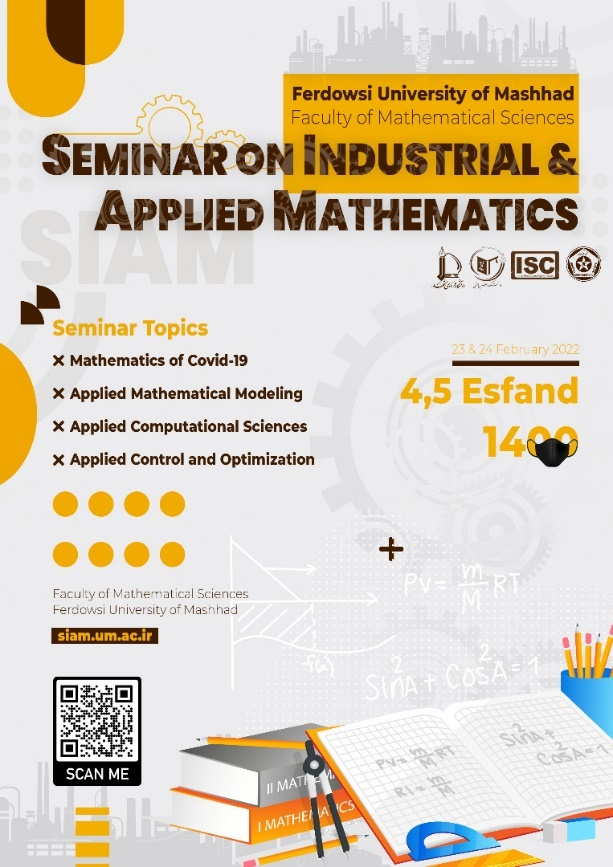
\includegraphics[keepaspectratio]{images/img_095.jpeg}}

}

\caption{image}

\end{figure}%

\begin{figure}[H]

{\centering \pandocbounded{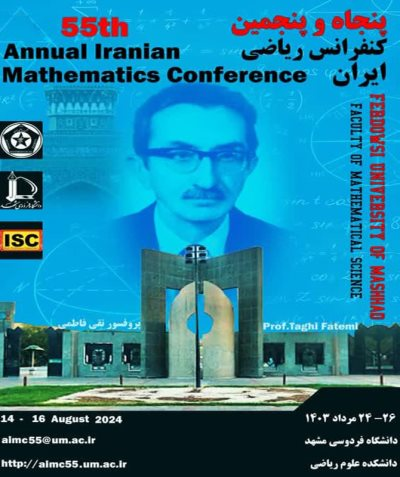
\includegraphics[keepaspectratio]{images/img_104.jpg}}

}

\caption{image}

\end{figure}%

\begin{figure}[H]

{\centering \pandocbounded{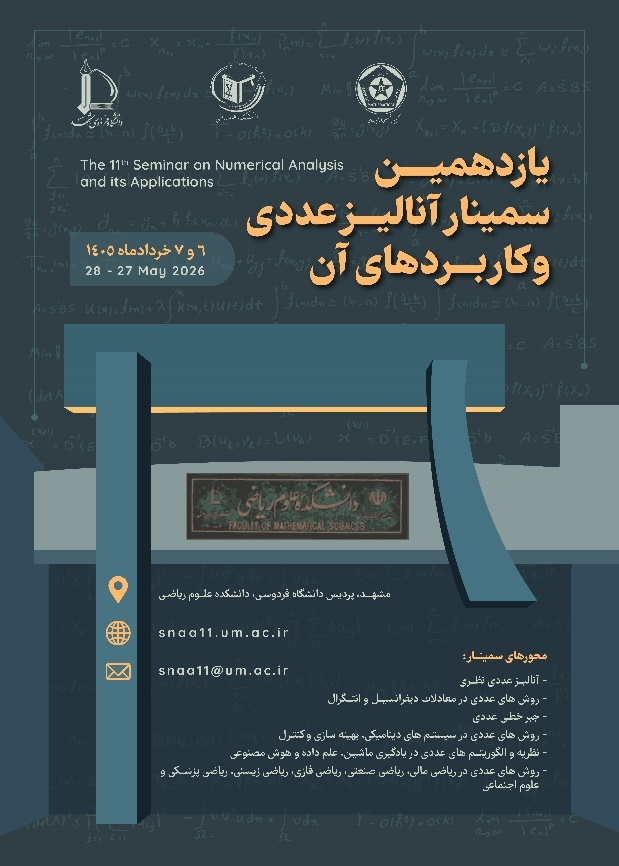
\includegraphics[keepaspectratio]{images/img_028.jpeg}}

}

\caption{image}

\end{figure}%

\begin{figure}[H]

{\centering \pandocbounded{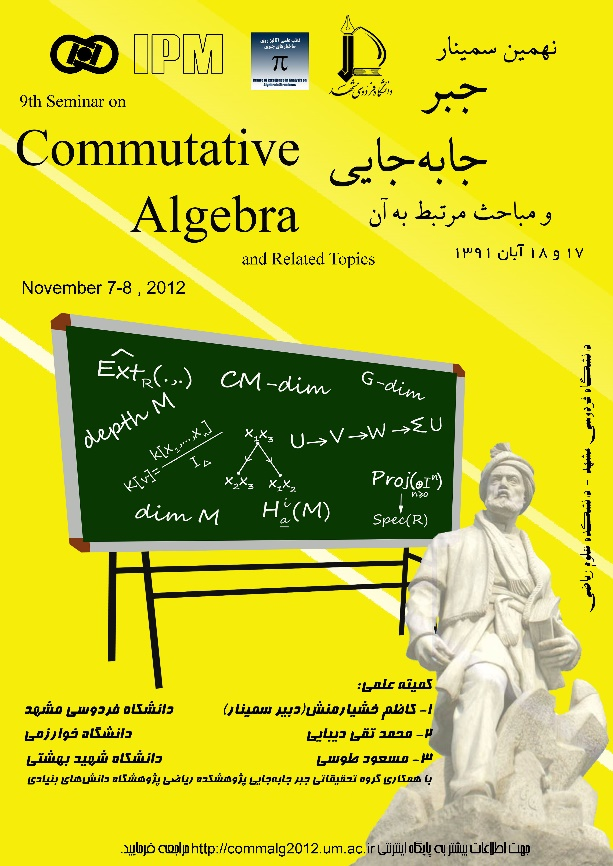
\includegraphics[keepaspectratio]{images/img_054.jpeg}}

}

\caption{image}

\end{figure}%

\begin{figure}[H]

{\centering \pandocbounded{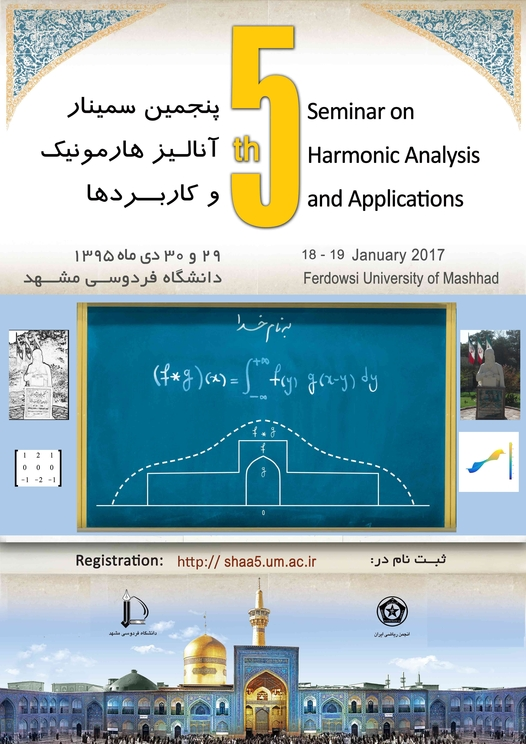
\includegraphics[keepaspectratio]{images/img_071.jpg}}

}

\caption{image}

\end{figure}%

\begin{figure}[H]

{\centering \pandocbounded{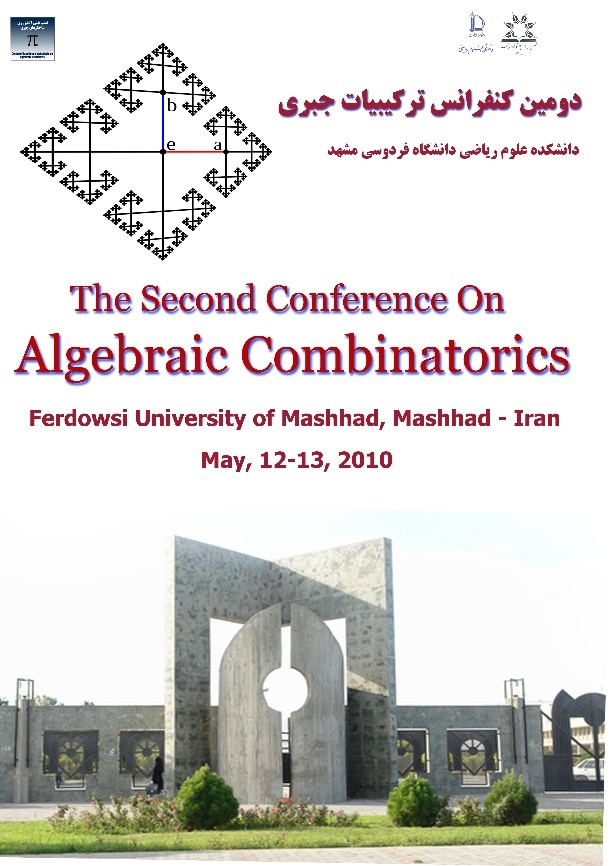
\includegraphics[keepaspectratio]{images/img_002.jpeg}}

}

\caption{image}

\end{figure}%

\begin{figure}[H]

{\centering \pandocbounded{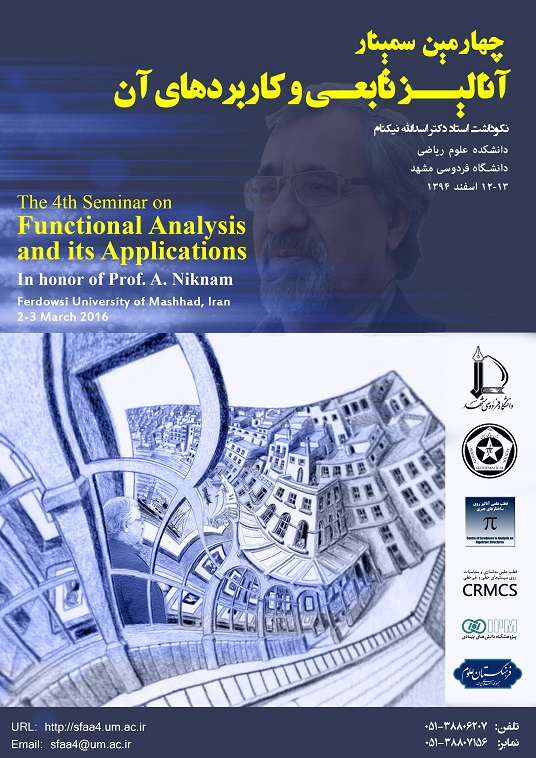
\includegraphics[keepaspectratio]{images/img_016.jpg}}

}

\caption{image}

\end{figure}%

\begin{figure}[H]

{\centering \pandocbounded{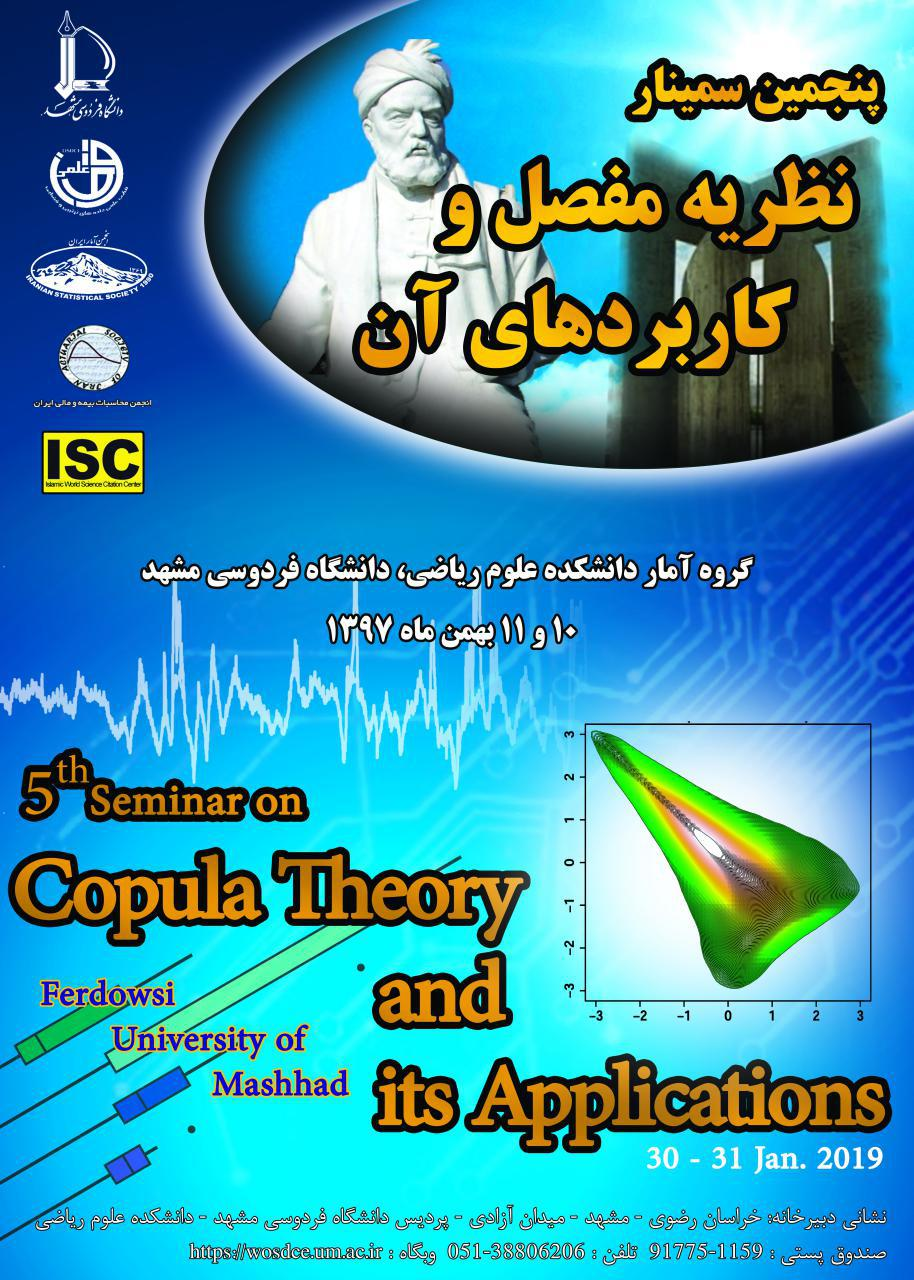
\includegraphics[keepaspectratio]{images/img_029.jpg}}

}

\caption{image}

\end{figure}%

\begin{figure}[H]

{\centering \pandocbounded{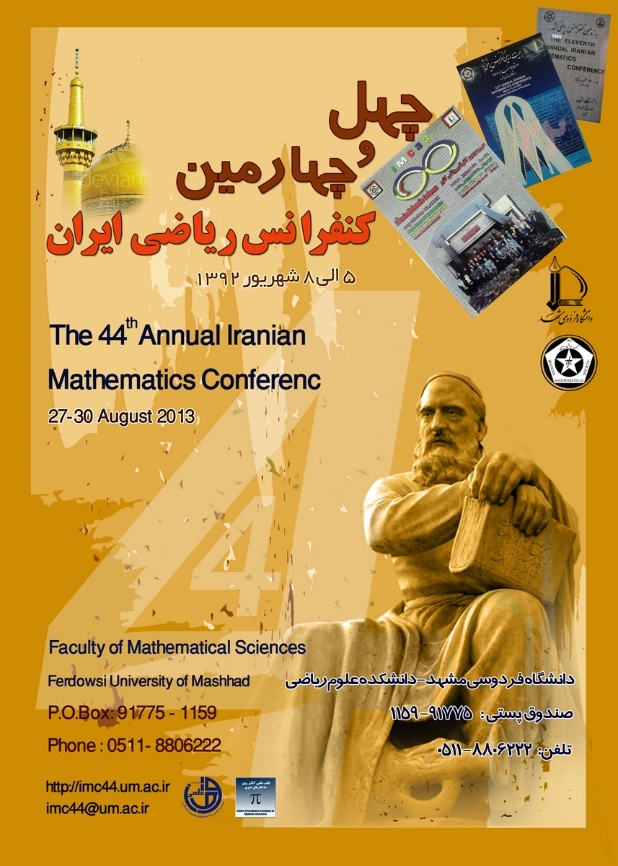
\includegraphics[keepaspectratio]{images/img_047.jpeg}}

}

\caption{image}

\end{figure}%

\begin{figure}[H]

{\centering \pandocbounded{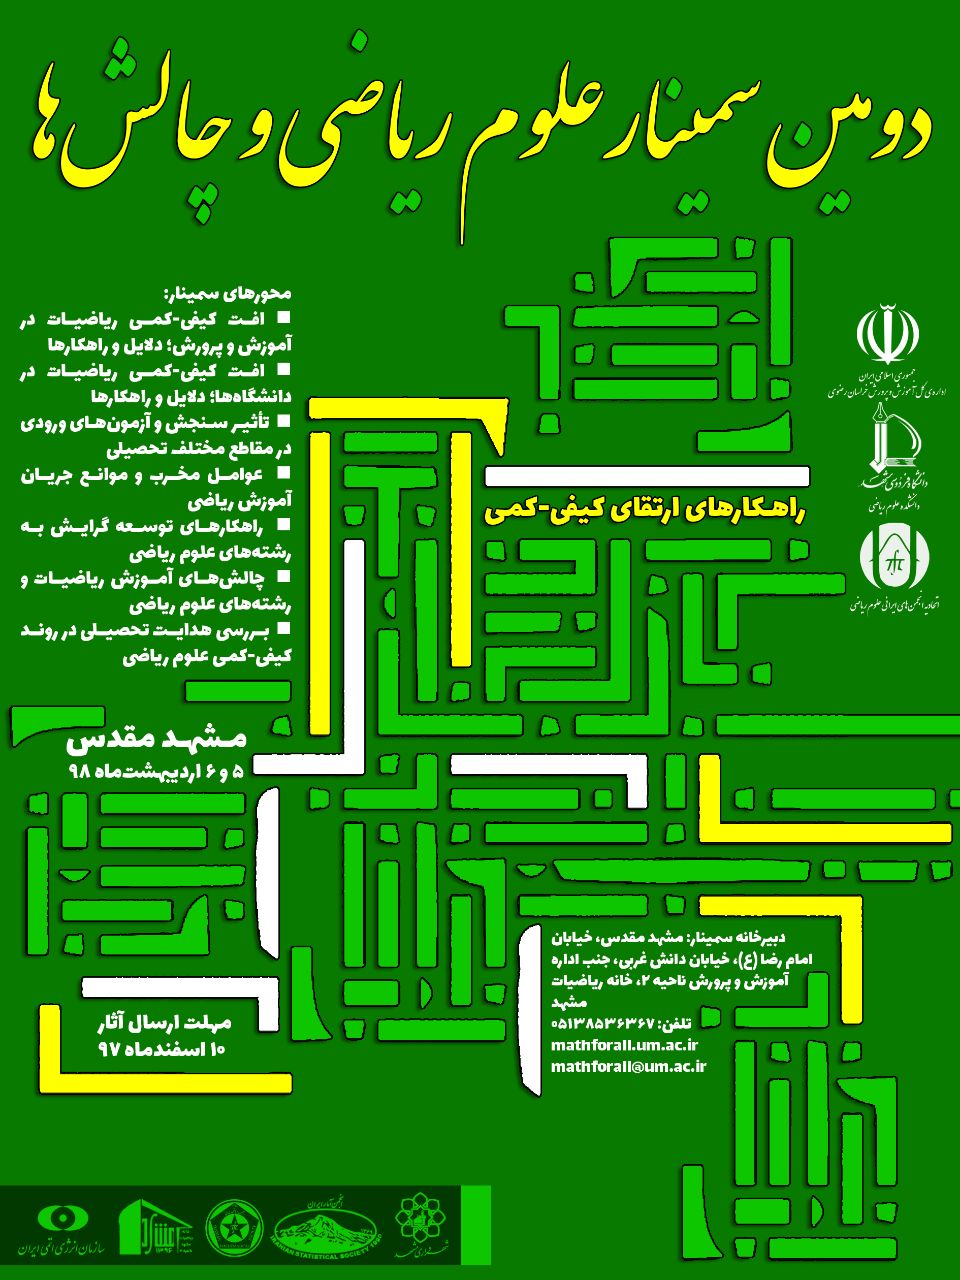
\includegraphics[keepaspectratio]{images/img_072.jpg}}

}

\caption{image}

\end{figure}%

\begin{figure}[H]

{\centering \pandocbounded{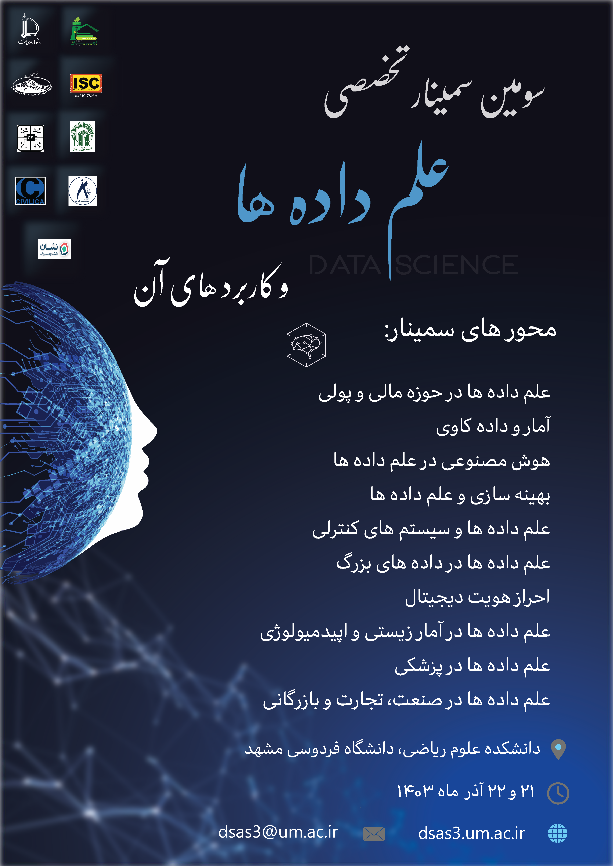
\includegraphics[keepaspectratio]{images/img_091.png}}

}

\caption{image}

\end{figure}%

\begin{figure}[H]

{\centering \pandocbounded{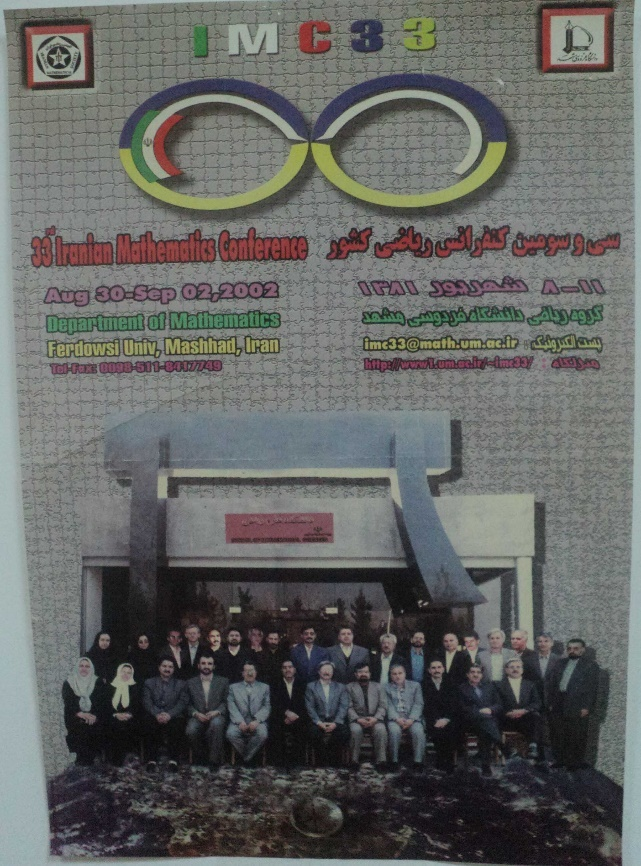
\includegraphics[keepaspectratio]{images/img_099.jpeg}}

}

\caption{image}

\end{figure}%

\begin{figure}[H]

{\centering \pandocbounded{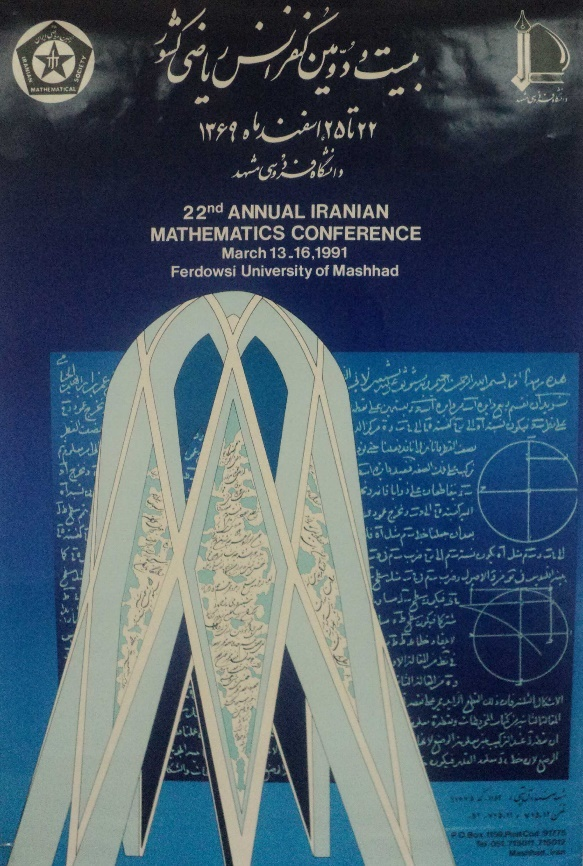
\includegraphics[keepaspectratio]{images/img_109.jpeg}}

}

\caption{image}

\end{figure}%

\begin{figure}[H]

{\centering \pandocbounded{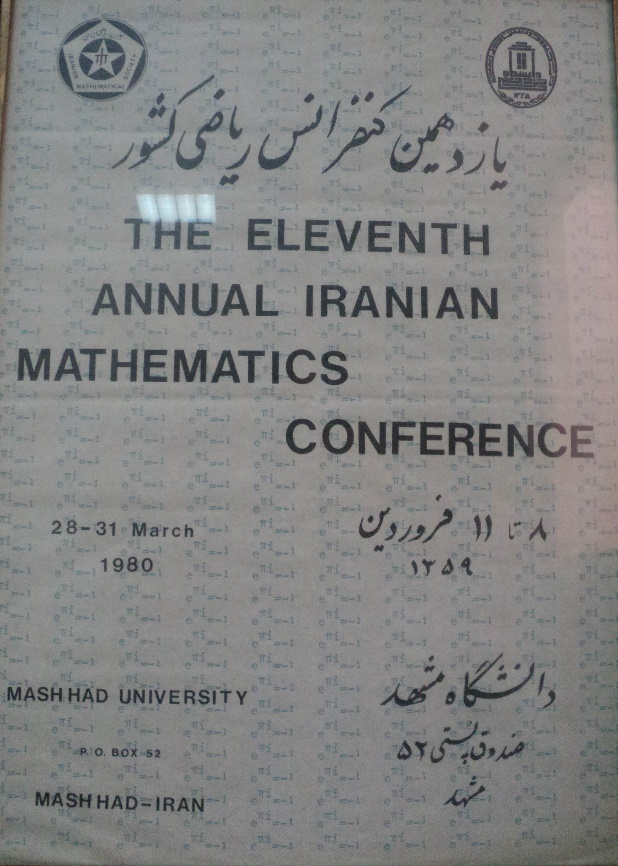
\includegraphics[keepaspectratio]{images/img_045.jpeg}}

}

\caption{image}

\end{figure}%

\begin{figure}[H]

{\centering \pandocbounded{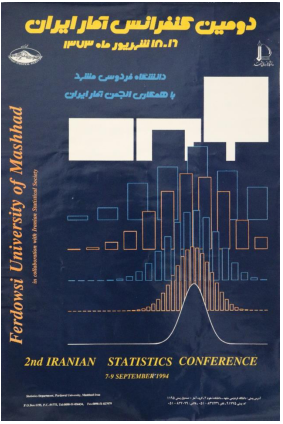
\includegraphics[keepaspectratio]{images/img_063.png}}

}

\caption{image}

\end{figure}%

\begin{figure}[H]

{\centering \pandocbounded{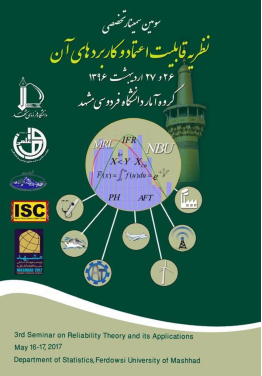
\includegraphics[keepaspectratio]{images/img_081.png}}

}

\caption{image}

\end{figure}%

\begin{figure}[H]

{\centering \pandocbounded{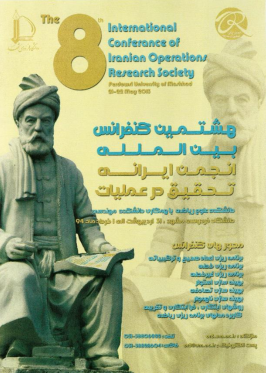
\includegraphics[keepaspectratio]{images/img_011.png}}

}

\caption{image}

\end{figure}%

\begin{figure}[H]

{\centering \pandocbounded{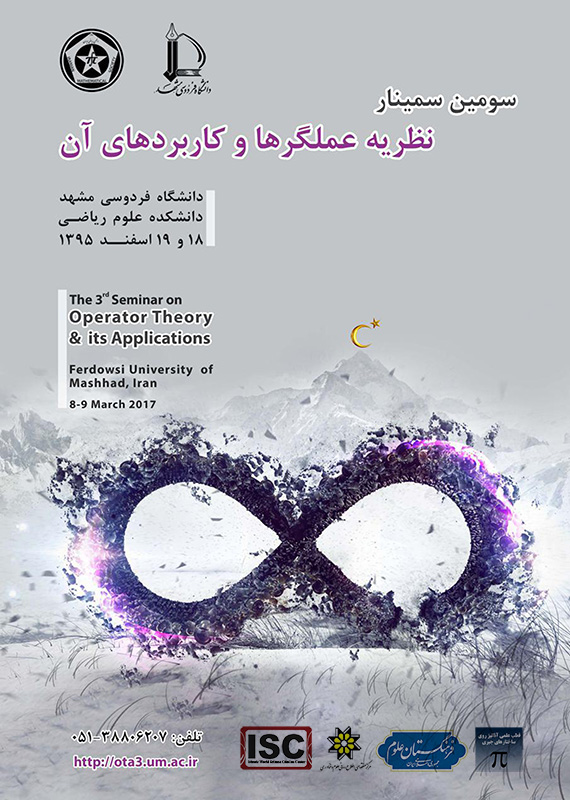
\includegraphics[keepaspectratio]{images/img_023.jpg}}

}

\caption{image}

\end{figure}%

\begin{figure}[H]

{\centering \pandocbounded{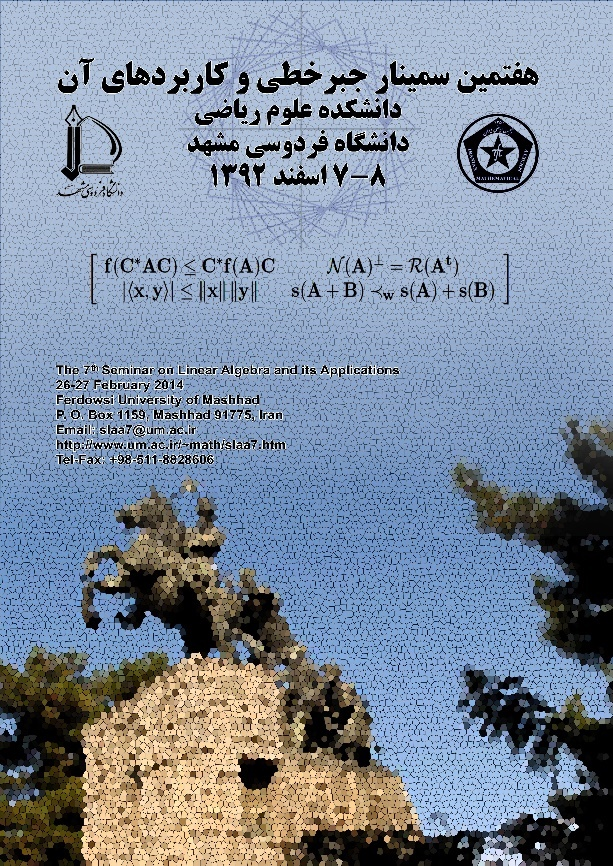
\includegraphics[keepaspectratio]{images/img_037.jpeg}}

}

\caption{image}

\end{figure}%

\begin{figure}[H]

{\centering \pandocbounded{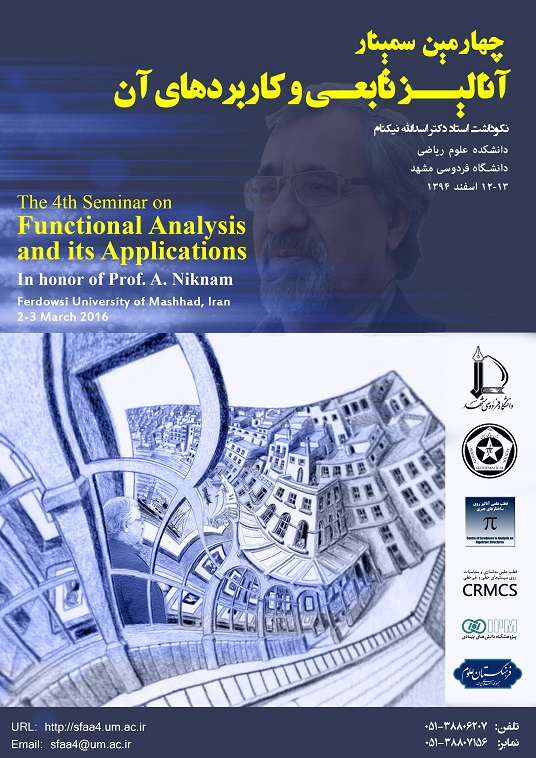
\includegraphics[keepaspectratio]{images/img_016.jpg}}

}

\caption{image}

\end{figure}%

\bookmarksetup{startatroot}

\chapter{نکوداشت‌ها و
بزرگداشت‌ها}\label{ux646ux6a9ux648ux62fux627ux634ux62aux647ux627-ux648-ux628ux632ux631ux6afux62fux627ux634ux62aux647ux627}

\bookmarksetup{startatroot}

\chapter{نکوداشت‌ها و
بزرگداشت‌ها}\label{ux646ux6a9ux648ux62fux627ux634ux62aux647ux627-ux648-ux628ux632ux631ux6afux62fux627ux634ux62aux647ux627-1}

{\def\LTcaptype{none} % do not increment counter
\begin{longtable}[]{@{}ll@{}}
\toprule\noalign{}
استاد پیشکسوت & تاریخ برگزاری \\
\midrule\noalign{}
\endhead
\bottomrule\noalign{}
\endlastfoot
پروفسور تقی فاطمی & ۱۵ اردیبهشت ماه ۱۳۷۹ \\
دکتر ابوالقاسم بزرگ نیا & ۲۸ اردیبهشت ماه ۱۳۸۴ \\
دکتر غلامحسین شاهکار & ۳۰ دی ماه ۱۳۹۴ \\
دکتر اسدالله نیکنام & ۱۲ اسفند ماه ۱۳۹۴ \\
دکتر بهمن هنری & ۲۴ آذر ماه ۱۳۹۵ \\
دکتر محمدعلی پورعبدالله‌نژاد & ۲۹ دی ماه ۱۳۹۵ \\
دکتر علی وحیدیان کامیاد & ۲۰ مهر ماه ۱۳۹۶ \\
دکتر ناصررضا ارقامی & ۱۹ اردیبهشت ماه ۱۳۹۷ \\
دکتر حسن صادقی & ۲ آبان ماه ۱۳۹۷ \\
دکتر حسنعلی آذرنوش & ۸ آبان ماه ۱۳۹۸ \\
دکتر فائزه توتونیان & ۱۳ دی ماه ۱۴۰۰ \\
دکتر شیرین حجازیان & ۲۱ اردیبهشت ماه ۱۴۰۱ \\
دکتر علی مشکانی & ۴ آبان ماه ۱۴۰۱ \\
دکتر حسینعلی نیرومند & ۳ آبان ماه ۱۴۰۲ \\
دکتر اصغر کرایه چیان & ۱۷ اردیبهشت ماه ۱۴۰۳ \\
دکتر طباطبایی & ۲ آبان ماه ۱۴۰۳ \\
دکتر محمدهادی فراهی & ۳ دی ماه ۱۴۰۳ \\
دکتر زهرا افشارنژاد & ۱۰ خرداد ماه ۱۴۰۴ \\
دکتر محمدرضا رجب زاده مقدم & ۹ مهر ماه ۱۴۰۴ \\
دکتر جعفر صابری نجفی & ۱۷ آذر ماه ۱۴۰۴ \\
\end{longtable}
}

\begin{figure}[H]

{\centering \pandocbounded{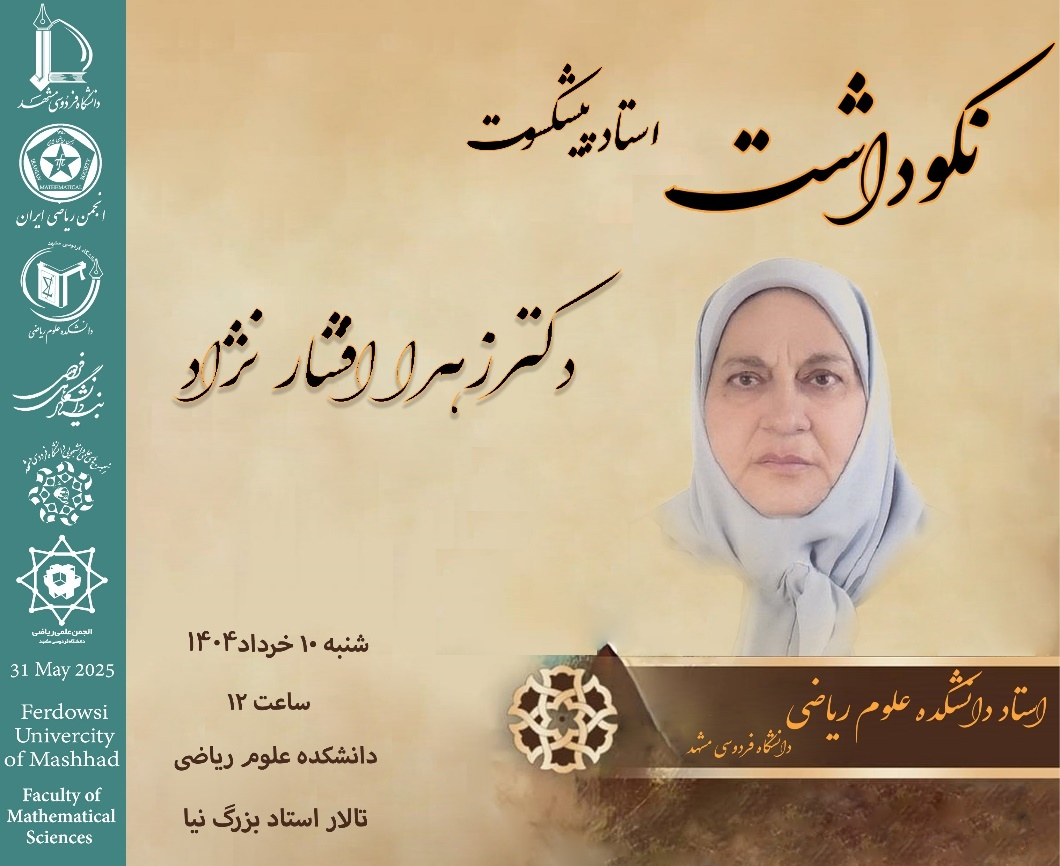
\includegraphics[keepaspectratio]{images/img_064.jpeg}}

}

\caption{image}

\end{figure}%

\begin{figure}[H]

{\centering \pandocbounded{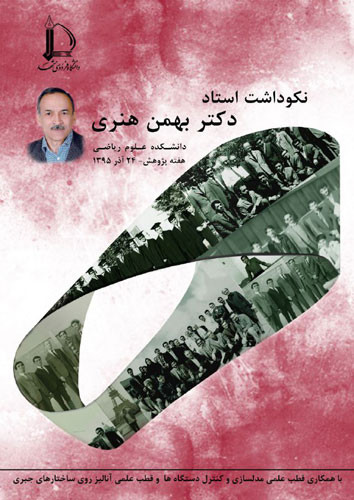
\includegraphics[keepaspectratio]{images/img_082.jpg}}

}

\caption{image}

\end{figure}%

\begin{figure}[H]

{\centering \pandocbounded{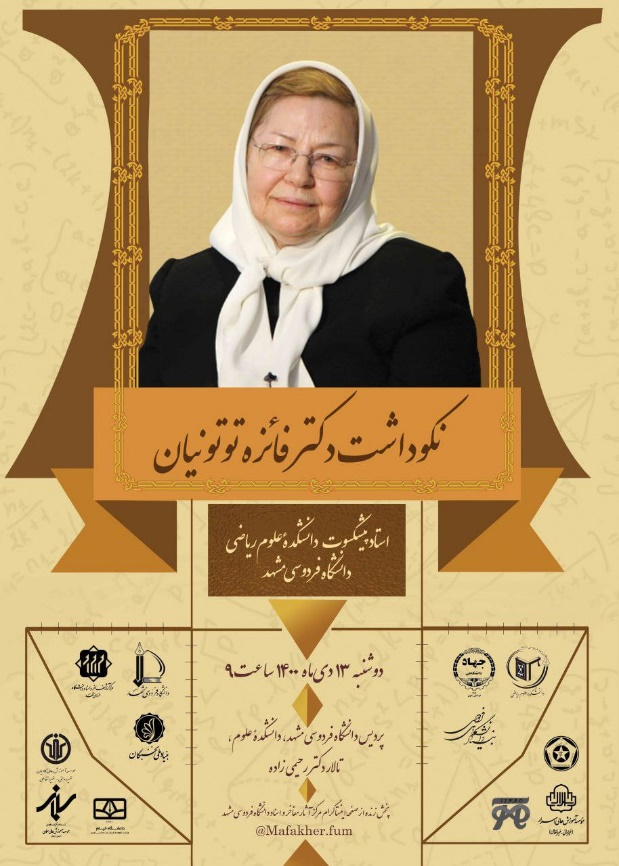
\includegraphics[keepaspectratio]{images/img_057.jpeg}}

}

\caption{image}

\end{figure}%

\begin{figure}[H]

{\centering \pandocbounded{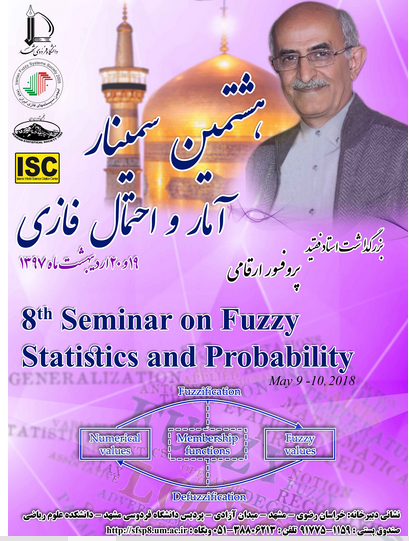
\includegraphics[keepaspectratio]{images/img_083.png}}

}

\caption{image}

\end{figure}%

\begin{figure}[H]

{\centering \pandocbounded{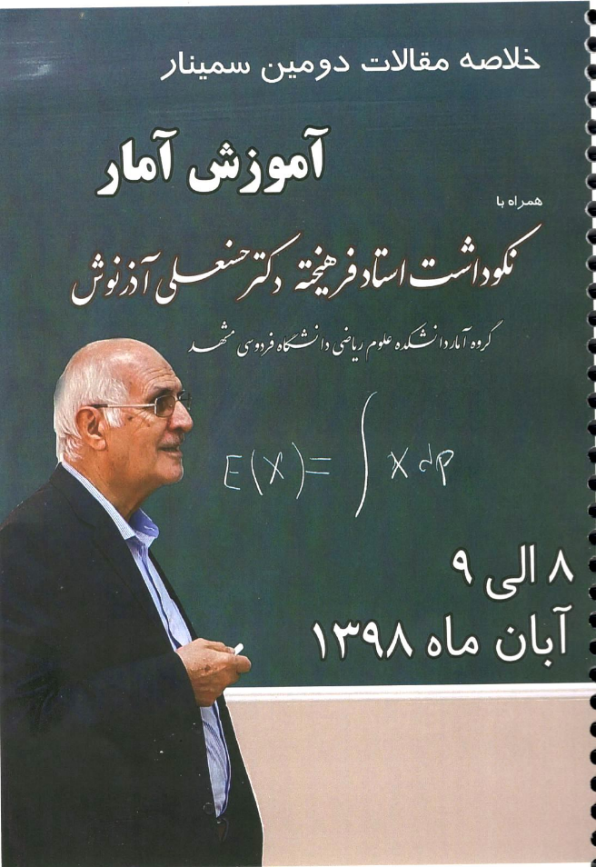
\includegraphics[keepaspectratio]{images/img_096.png}}

}

\caption{image}

\end{figure}%

\begin{figure}[H]

{\centering \pandocbounded{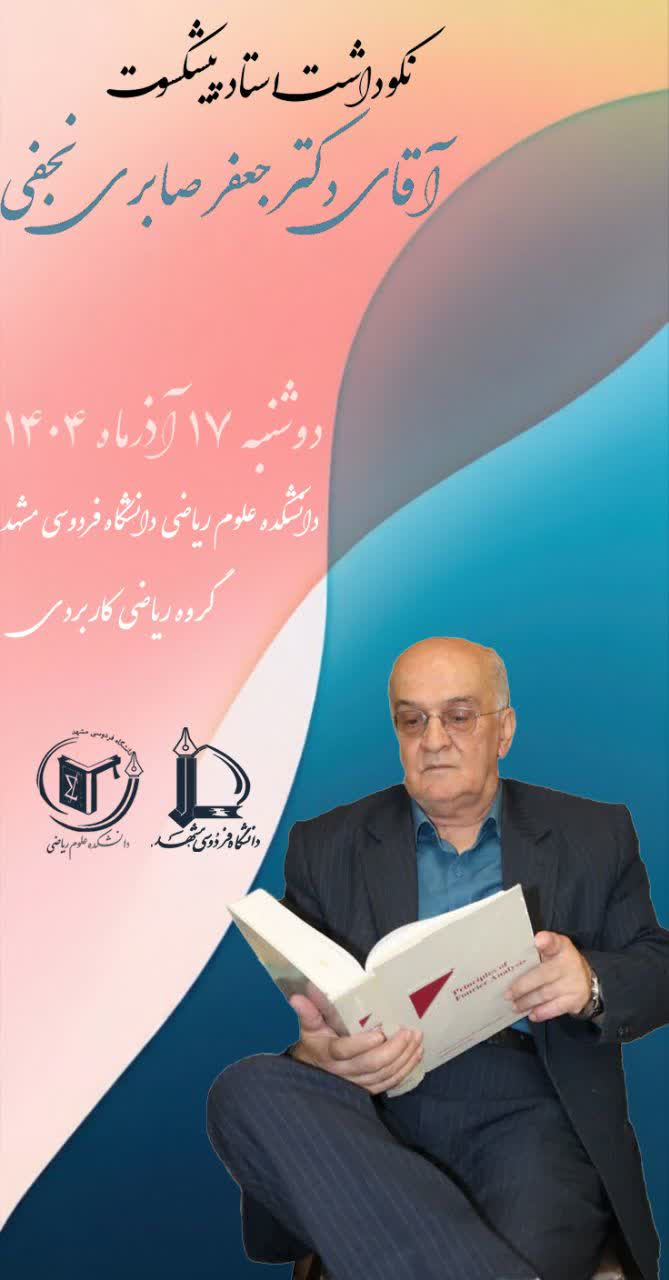
\includegraphics[keepaspectratio]{images/img_106.jpg}}

}

\caption{image}

\end{figure}%

\begin{figure}[H]

{\centering \pandocbounded{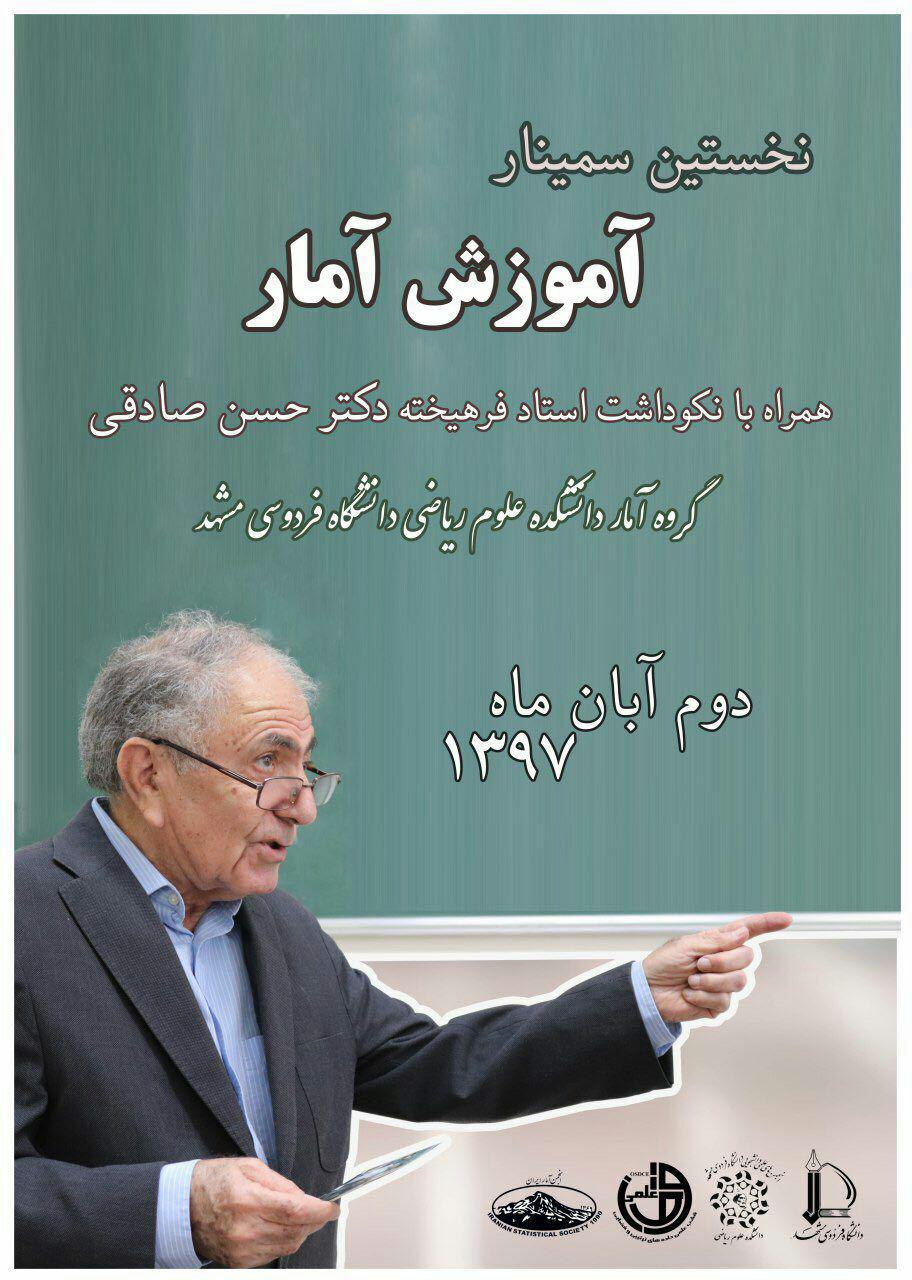
\includegraphics[keepaspectratio]{images/img_038.jpg}}

}

\caption{image}

\end{figure}%

\begin{figure}[H]

{\centering \pandocbounded{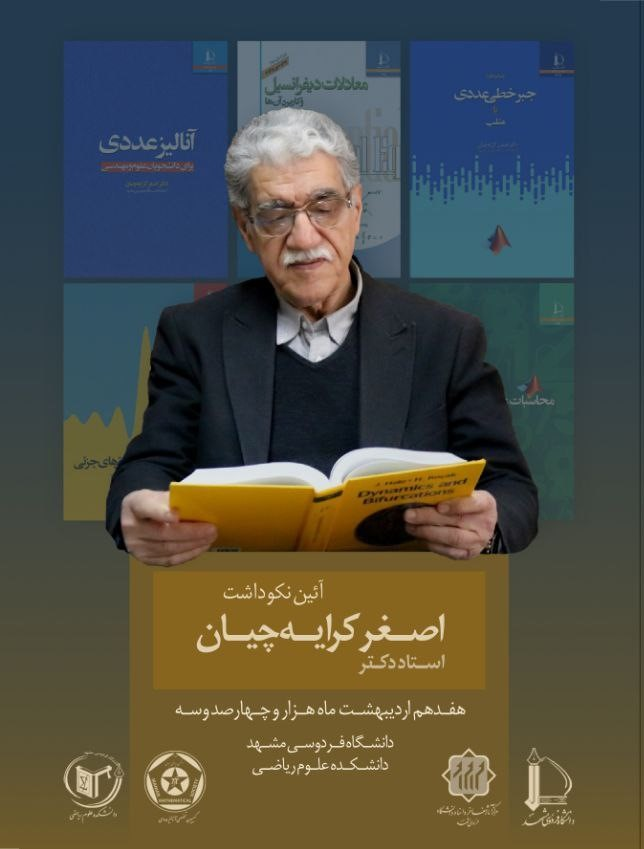
\includegraphics[keepaspectratio]{images/img_058.jpg}}

}

\caption{image}

\end{figure}%

\begin{figure}[H]

{\centering \pandocbounded{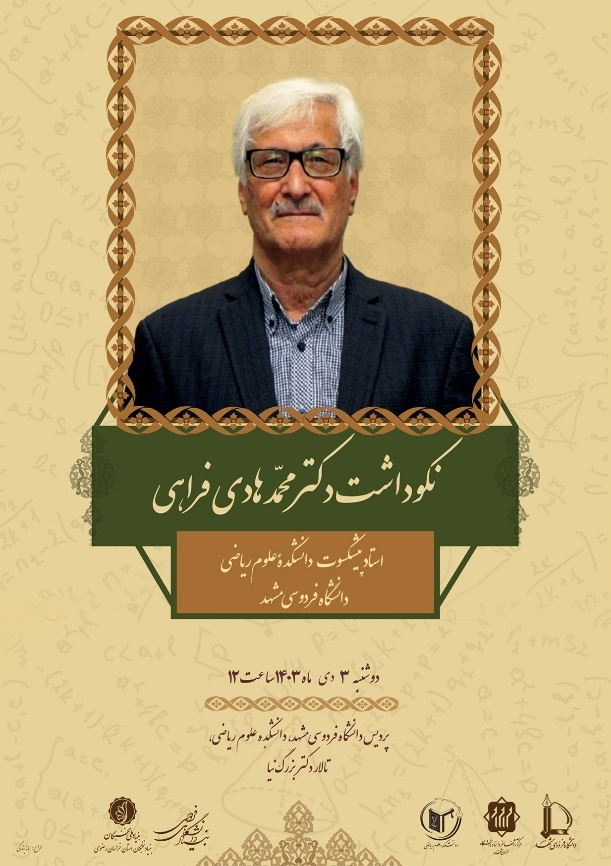
\includegraphics[keepaspectratio]{images/img_077.jpeg}}

}

\caption{image}

\end{figure}%

\begin{figure}[H]

{\centering \pandocbounded{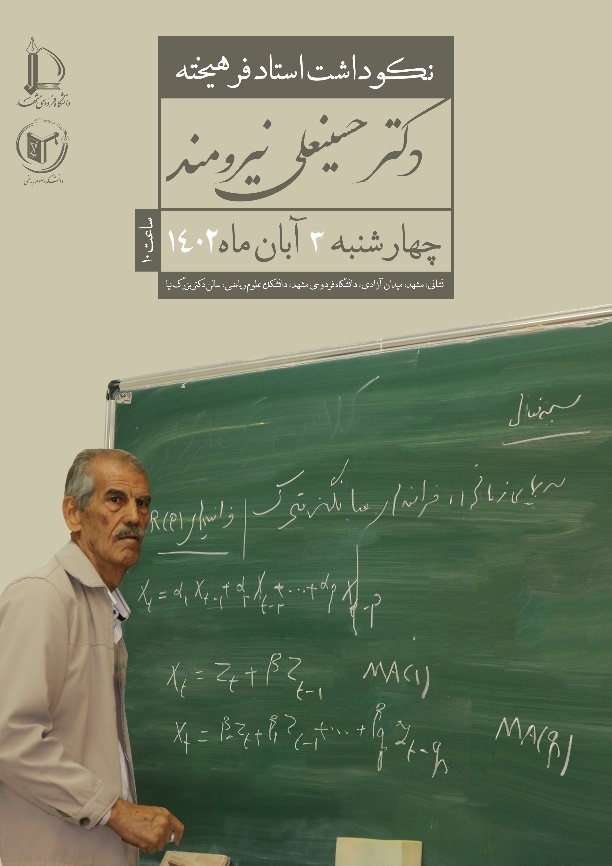
\includegraphics[keepaspectratio]{images/img_006.jpeg}}

}

\caption{image}

\end{figure}%

\begin{figure}[H]

{\centering \pandocbounded{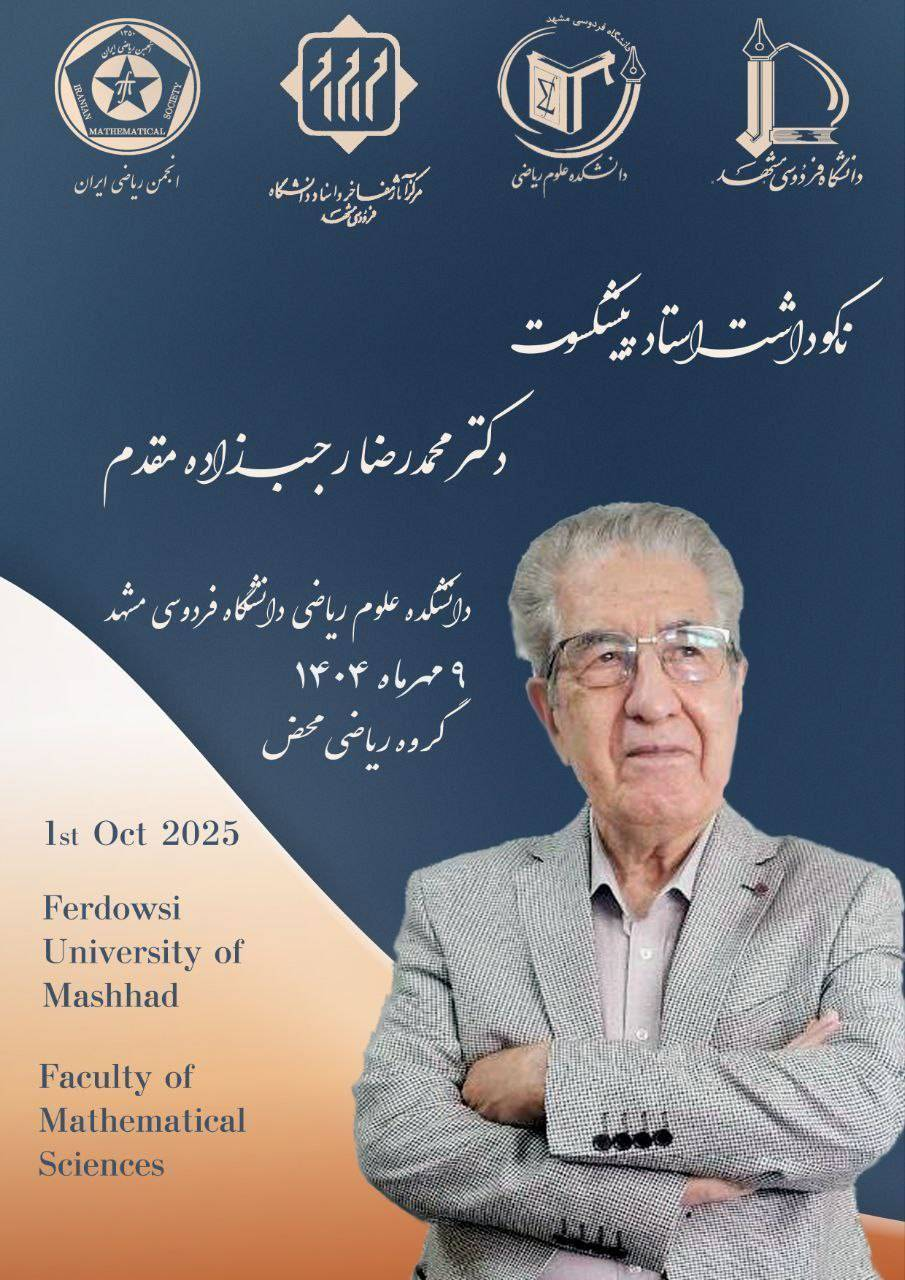
\includegraphics[keepaspectratio]{images/img_020.jpg}}

}

\caption{image}

\end{figure}%

\bookmarksetup{startatroot}

\chapter{کتاب‌ها}\label{ux6a9ux62aux627ux628ux647ux627}

\bookmarksetup{startatroot}

\chapter{کتاب‌ها}\label{ux6a9ux62aux627ux628ux647ux627-1}

دکتر حسنعلی آذرنوش

{\def\LTcaptype{none} % do not increment counter
\begin{longtable}[]{@{}lll@{}}
\toprule\noalign{}
\# & عنوان کتاب & نوع اثر \\
\midrule\noalign{}
\endhead
\bottomrule\noalign{}
\endlastfoot
۱ & روش‌های جایگزین در رگرسیون & ترجمه \\
۲ & نظریه اطلاع & ترجمه \\
۳ & نخستین درس احتمال & ترجمه \\
۴ & مدل‌های خطی برای آمار & ترجمه \\
۵ & نخستین درس آماره‌های تربیتی & ترجمه \\
۶ & نخستین درس در طرح آزمایش‌ها & ترجمه \\
۷ & تجزیه و تحلیل سری‌های زمانی & ترجمه \\
۸ & شبیه‌سازی & ترجمه \\
\end{longtable}
}

دکتر محمد آرشی

{\def\LTcaptype{none} % do not increment counter
\begin{longtable}[]{@{}
  >{\raggedright\arraybackslash}p{(\linewidth - 4\tabcolsep) * \real{0.3333}}
  >{\raggedright\arraybackslash}p{(\linewidth - 4\tabcolsep) * \real{0.3333}}
  >{\raggedright\arraybackslash}p{(\linewidth - 4\tabcolsep) * \real{0.3333}}@{}}
\toprule\noalign{}
\begin{minipage}[b]{\linewidth}\raggedright
\#
\end{minipage} & \begin{minipage}[b]{\linewidth}\raggedright
عنوان کتاب
\end{minipage} & \begin{minipage}[b]{\linewidth}\raggedright
نوع اثر
\end{minipage} \\
\midrule\noalign{}
\endhead
\bottomrule\noalign{}
\endlastfoot
۱ & استنباط آماری (با رویکرد برآورد نقطه‌ای) & تدوین و گردآوری \\
۲ & Statistical Inference for Models with Multivariate t-Distributed
Errors & تصنیف \\
۳ & Theory of Ridge Regression Estimation with Applications & تصنیف \\
۴ & Rank-Based Methods for Shrinkage and Selection: with Application to
Machine Learning & تصنیف \\
۵ & Innovations in Multivariate Statistical Modeling: Navigating
Theoretical and Multidisciplinary Domains & تصنیف \\
۶ & Computational and Methodological Statistics and Biostatistics -
Contemporary Essays in Advancement & تصنیف \\
۷ & Directional Statistics for Innovative Applications. A Bicentennial
Tribute to Florence Nightingale & تصنیف \\
۸ & Flexible Nonparametric Curve Estimation & تألیف \\
۹ & Directional and Multivariate Statistics & تألیف \\
۱۰ & Advances in Shrinkage and Penalized Estimation Strategies & تدوین و
گردآوری \\
\end{longtable}
}

دکتر ناصررضا ارقامی

{\def\LTcaptype{none} % do not increment counter
\begin{longtable}[]{@{}lll@{}}
\toprule\noalign{}
\# & عنوان کتاب & نوع اثر \\
\midrule\noalign{}
\endhead
\bottomrule\noalign{}
\endlastfoot
۱ & شواهد آماری & ترجمه \\
۲ & مقدمه‌ای بر بررسی‌های نمونه‌ای & ترجمه \\
\end{longtable}
}

دکتر زهرا افشارنژاد

{\def\LTcaptype{none} % do not increment counter
\begin{longtable}[]{@{}lll@{}}
\toprule\noalign{}
\# & عنوان کتاب & نوع اثر \\
\midrule\noalign{}
\endhead
\bottomrule\noalign{}
\endlastfoot
۱ & معادلات دیفرانسیل و معادلات با مشتقات جزئی مقدماتی & تألیف \\
۲ & آنالیز ریاضی ۳ و کاربردهای آن & گردآوری و تدوین \\
\end{longtable}
}

دکتر محمود امین‌طوسی

{\def\LTcaptype{none} % do not increment counter
\begin{longtable}[]{@{}lll@{}}
\toprule\noalign{}
\# & عنوان کتاب & نوع اثر \\
\midrule\noalign{}
\endhead
\bottomrule\noalign{}
\endlastfoot
۱ & مقدمه‌ای بر زی‌پرشین و ریاضی‌نویسی در لاتک & تصنیف \\
\end{longtable}
}

دکتر محمد امینی

{\def\LTcaptype{none} % do not increment counter
\begin{longtable}[]{@{}lll@{}}
\toprule\noalign{}
\# & عنوان کتاب & نوع اثر \\
\midrule\noalign{}
\endhead
\bottomrule\noalign{}
\endlastfoot
۱ & مقدمه‌ای بر زمین‌آمار & ویراستاری علمی \\
۲ & مقدمه‌ای بر سری‌های زمانی و پیش‌بینی & ترجمه \\
۳ & مقدمه‌ای بر فرایندهای تصادفی & ترجمه \\
۴ & نظریه احتمال & تألیف \\
۵ & فرایندهای تصادفی با نرم‌افزار آر & ترجمه \\
۶ & آمار با نرم‌افزار JMP: نمودارها، آمار توصیفی و احتمال & ترجمه \\
\end{longtable}
}

دکتر سید حسین اورعی

{\def\LTcaptype{none} % do not increment counter
\begin{longtable}[]{@{}lll@{}}
\toprule\noalign{}
\# & عنوان کتاب & نوع اثر \\
\midrule\noalign{}
\endhead
\bottomrule\noalign{}
\endlastfoot
۱ & حساب دیفرانسیل و انتگرال (جلد اول) & ترجمه \\
۲ & حساب دیفرانسیل و انتگرال (جلد دوم) & ترجمه \\
\end{longtable}
}

دکتر ابوالقاسم بزرگ‌نیا

{\def\LTcaptype{none} % do not increment counter
\begin{longtable}[]{@{}
  >{\raggedright\arraybackslash}p{(\linewidth - 6\tabcolsep) * \real{0.2500}}
  >{\raggedright\arraybackslash}p{(\linewidth - 6\tabcolsep) * \real{0.2500}}
  >{\raggedright\arraybackslash}p{(\linewidth - 6\tabcolsep) * \real{0.2500}}
  >{\raggedright\arraybackslash}p{(\linewidth - 6\tabcolsep) * \real{0.2500}}@{}}
\toprule\noalign{}
\begin{minipage}[b]{\linewidth}\raggedright
\#
\end{minipage} & \begin{minipage}[b]{\linewidth}\raggedright
عنوان کتاب
\end{minipage} & \begin{minipage}[b]{\linewidth}\raggedright
نوع اثر
\end{minipage} & \begin{minipage}[b]{\linewidth}\raggedright
جایزه /برگزیده
\end{minipage} \\
\midrule\noalign{}
\endhead
\bottomrule\noalign{}
\endlastfoot
۱ & تجزیه و تحلیل سری‌های زمانی و پیش‌بینی & ترجمه & \\
۲ & الگوهای آماری گسسته و کاربرد آن در علوم اجتماعی & ترجمه & \\
۳ & کاربرد الگوهای احتمال & ترجمه & \\
۴ & حل المسائل آنالیز & تألیف & \\
۵ & مقدمه‌ای بر فرایندهای تصادفی & ترجمه & \\
۶ & الگوریتمهای عددی: محاسبات در علوم و مهندسی & ترجمه & \\
۷ & ریاضیات مهندسی & ترجمه & \\
۸ & مقدمه‌ای بر آمار و احتمال (برای مهندسان و محققان علوم) & ترجمه & \\
۹ & تحلیل بقا & ترجمه & \\
۱۰ & جبر خطی و کاربردهای آن & ترجمه & \\
۱۱ & نظریه آمار & ترجمه & برگزیده کتاب سال جمهوری اسلامی ایران، دوره
هفتم ۱۳۶۷ \\
۱۲ & سریهای زمانی (رشد آمار) & تألیف & \\
۱۳ & تحلیل رگرسیون غیرخطی و کاربردهای آن & ترجمه & \\
۱۴ & تحلیل فراوانی وقایع و ریسک در هیدرولوژی & ترجمه & \\
۱۵ & مبانی فیزیک ریاضی (همراه با تقی عدالتی) & ترجمه & \\
۱۶ & مقدمه‌ای بر تحلیل سری‌های زمانی & ترجمه & \\
\end{longtable}
}

دکتر محمدعلی پورعبدالله

{\def\LTcaptype{none} % do not increment counter
\begin{longtable}[]{@{}lll@{}}
\toprule\noalign{}
\# & عنوان کتاب & نوع اثر \\
\midrule\noalign{}
\endhead
\bottomrule\noalign{}
\endlastfoot
۱ & منطق برای ریاضیدانان & ترجمه \\
۲ & شناخت عمومی علم & ترجمه \\
\end{longtable}
}

دکتر حسین تقی‌زاده کاخکی

{\def\LTcaptype{none} % do not increment counter
\begin{longtable}[]{@{}lll@{}}
\toprule\noalign{}
\# & عنوان کتاب & نوع اثر \\
\midrule\noalign{}
\endhead
\bottomrule\noalign{}
\endlastfoot
۱ & برنامه‌ریزی ریاضی کاربردی & ترجمه \\
۲ & بهینه‌سازی خطی & تألیف \\
\end{longtable}
}

دکتر فائزه توتونیان

{\def\LTcaptype{none} % do not increment counter
\begin{longtable}[]{@{}
  >{\raggedright\arraybackslash}p{(\linewidth - 6\tabcolsep) * \real{0.2500}}
  >{\raggedright\arraybackslash}p{(\linewidth - 6\tabcolsep) * \real{0.2500}}
  >{\raggedright\arraybackslash}p{(\linewidth - 6\tabcolsep) * \real{0.2500}}
  >{\raggedright\arraybackslash}p{(\linewidth - 6\tabcolsep) * \real{0.2500}}@{}}
\toprule\noalign{}
\begin{minipage}[b]{\linewidth}\raggedright
\#
\end{minipage} & \begin{minipage}[b]{\linewidth}\raggedright
عنوان کتاب
\end{minipage} & \begin{minipage}[b]{\linewidth}\raggedright
نوع اثر
\end{minipage} & \begin{minipage}[b]{\linewidth}\raggedright
جایزه /برگزیده
\end{minipage} \\
\midrule\noalign{}
\endhead
\bottomrule\noalign{}
\endlastfoot
۱ & آنالیز عددی ۱ و ۲ & ترجمه & کتاب برگزیده فرهنگ و ارشاد اسلامی و
جشنواره دانشگاه فردوسی مشهد \\
۲ & جبر خطی عددی و کاربردها ۱ و ۲ & ترجمه & کتاب برگزیده جشنواره دانشگاه
فردوسی مشهد- آذر ۱۳۸۸، هفته پژوهش- رتبه سوم \\
۳ & الگوریتم‌های عددی & ترجمه & کتاب برگزیده جشنواره دانشگاه تهران \\
۴ & برنامه‌ریزی خطی & ترجمه & کتاب برگزیده جشنواره دانشگاه تهران ( کتاب
سال دانشگاهها ۱۳۶۹) \\
۵ & روش‌های محاسبات عددی & ترجمه & \\
۶ & برنامه‌ریزی خطی (روش‌ها و کاربرد) & ترجمه & \\
۷ & مقدمه‌ای بر محاسبات علمی & ترجمه & \\
۸ & ماتریس و جبر خطی & ترجمه & \\
\end{longtable}
}

دکتر مصطفی توکلی

{\def\LTcaptype{none} % do not increment counter
\begin{longtable}[]{@{}lll@{}}
\toprule\noalign{}
\# & عنوان کتاب & نوع اثر \\
\midrule\noalign{}
\endhead
\bottomrule\noalign{}
\endlastfoot
۱ & نظریه گراف و کاربردهای آن & تألیف \\
۲ & گراف‌های وابسته به برخی از ساختارهای جبری & ویراستاری علمی \\
۳ & اعمال گراف و کاربرد آنها در ریاضی-شیمی & تصنیف \\
۴ & الگوریتم‌های گراف: از تئوری تا پیاده‌سازی & تألیف \\
۵ & نظریه گراف و کاربردهای آن & تألیف \\
\end{longtable}
}

دکتر محمد جانفدا

{\def\LTcaptype{none} % do not increment counter
\begin{longtable}[]{@{}lll@{}}
\toprule\noalign{}
\# & عنوان کتاب & نوع اثر \\
\midrule\noalign{}
\endhead
\bottomrule\noalign{}
\endlastfoot
۱ & آنالیز حقیقی با مقدمه‌ای بر موجک و کاربردهای آن & ترجمه \\
\end{longtable}
}

دکتر مهدی جباری نوقابی

{\def\LTcaptype{none} % do not increment counter
\begin{longtable}[]{@{}
  >{\raggedright\arraybackslash}p{(\linewidth - 4\tabcolsep) * \real{0.3333}}
  >{\raggedright\arraybackslash}p{(\linewidth - 4\tabcolsep) * \real{0.3333}}
  >{\raggedright\arraybackslash}p{(\linewidth - 4\tabcolsep) * \real{0.3333}}@{}}
\toprule\noalign{}
\begin{minipage}[b]{\linewidth}\raggedright
\#
\end{minipage} & \begin{minipage}[b]{\linewidth}\raggedright
عنوان کتاب
\end{minipage} & \begin{minipage}[b]{\linewidth}\raggedright
نوع اثر
\end{minipage} \\
\midrule\noalign{}
\endhead
\bottomrule\noalign{}
\endlastfoot
۱ & روش‌های پیشرفته آماری و مدل‌های خطی در علوم دامی (با استفاده از
نرم‌افزار R) & تألیف \\
۲ & روش‌های پیشرفته آماری و مدل‌های خطی در علوم دامی (با استفاده از
نرم‌افزار R) & تألیف \\
۳ & مقدمه‌ای بر برخی از آزمون‌های آماری در علوم کشاورزی با R & تألیف \\
۴ & آمار و تحلیل کاربردی داده‌ها (از مفاهیم پایه تا مدل‌های پیشرفته) همراه
با پیاده‌سازی مثال‌ها & تصنیف \\
\end{longtable}
}

دکتر هادی جباری نوقابی

{\def\LTcaptype{none} % do not increment counter
\begin{longtable}[]{@{}lll@{}}
\toprule\noalign{}
\# & عنوان کتاب & نوع اثر \\
\midrule\noalign{}
\endhead
\bottomrule\noalign{}
\endlastfoot
۱ & تعیین حجم نمونه با نرم‌افزار PASS & تألیف \\
\end{longtable}
}

دکتر کاظم چیتی

{\def\LTcaptype{none} % do not increment counter
\begin{longtable}[]{@{}lll@{}}
\toprule\noalign{}
\# & عنوان کتاب & نوع اثر \\
\midrule\noalign{}
\endhead
\bottomrule\noalign{}
\endlastfoot
۱ & حلقه‌ها، مدول‌ها و جبر خطی & ترجمه \\
\end{longtable}
}

دکتر کاظم خشیارمنش

{\def\LTcaptype{none} % do not increment counter
\begin{longtable}[]{@{}lll@{}}
\toprule\noalign{}
\# & عنوان کتاب & نوع اثر \\
\midrule\noalign{}
\endhead
\bottomrule\noalign{}
\endlastfoot
۱ & Commutative rings: New Research & تألیف \\
۲ & نظریه گراف و کاربردهای آن & ویراستاری علمی \\
۳ & گراف‌های وابسته به برخی از ساختارهای جبری & تصنیف \\
\end{longtable}
}

دکتر محمد خنجری صادق

{\def\LTcaptype{none} % do not increment counter
\begin{longtable}[]{@{}
  >{\raggedright\arraybackslash}p{(\linewidth - 4\tabcolsep) * \real{0.3333}}
  >{\raggedright\arraybackslash}p{(\linewidth - 4\tabcolsep) * \real{0.3333}}
  >{\raggedright\arraybackslash}p{(\linewidth - 4\tabcolsep) * \real{0.3333}}@{}}
\toprule\noalign{}
\begin{minipage}[b]{\linewidth}\raggedright
\#
\end{minipage} & \begin{minipage}[b]{\linewidth}\raggedright
عنوان کتاب
\end{minipage} & \begin{minipage}[b]{\linewidth}\raggedright
نوع اثر
\end{minipage} \\
\midrule\noalign{}
\endhead
\bottomrule\noalign{}
\endlastfoot
۱ & Statistical Modeling of Reliability Structures and Industrial
Processes & تألیف \\
\end{longtable}
}

دکتر رسول رمضانیان

{\def\LTcaptype{none} % do not increment counter
\begin{longtable}[]{@{}lll@{}}
\toprule\noalign{}
\# & عنوان کتاب & نوع اثر \\
\midrule\noalign{}
\endhead
\bottomrule\noalign{}
\endlastfoot
۱ & هوش اجتماعی & تألیف \\
۲ & Mathematics, Logic, and their Philosophies & تألیف \\
\end{longtable}
}

دکتر محمدرضا رجب‌زاده مقدم

{\def\LTcaptype{none} % do not increment counter
\begin{longtable}[]{@{}
  >{\raggedright\arraybackslash}p{(\linewidth - 4\tabcolsep) * \real{0.3333}}
  >{\raggedright\arraybackslash}p{(\linewidth - 4\tabcolsep) * \real{0.3333}}
  >{\raggedright\arraybackslash}p{(\linewidth - 4\tabcolsep) * \real{0.3333}}@{}}
\toprule\noalign{}
\begin{minipage}[b]{\linewidth}\raggedright
\#
\end{minipage} & \begin{minipage}[b]{\linewidth}\raggedright
عنوان کتاب
\end{minipage} & \begin{minipage}[b]{\linewidth}\raggedright
نوع اثر
\end{minipage} \\
\midrule\noalign{}
\endhead
\bottomrule\noalign{}
\endlastfoot
۱ & درسی در جبر خطی همراه با کاربردها & ترجمه \\
۲ & درسی در نظریه گالوا & ترجمه \\
۳ & حل المسائل درسی در جبر خطی همراه با کاربردها & ترجمه \\
۴ & نخستین درس در جبر مجرد & ترجمه \\
۵ & جبر خطی (همراه با ابوالقاسم بزرگ‌نیا) & ترجمه \\
۶ & اساس جبر مجرد (همراه با سید محمد داورپناه) & ترجمه \\
۷ & جبر مجرد (همراه با علی‌اکبر محمدی حسن‌آبادی) & ترجمه \\
۸ & مقدمه‌ای بر نظریه گروه‌های متناهی (همراه با حسن صادق‌پور) & ترجمه \\
۹ & آشنایی با نظریه گروه‌ها، حلقه‌ها، میدان‌ها و مدول‌ها (همراه با علیرضا
سالم‌کار) & تألیف \\
\end{longtable}
}

دکتر فریدون رهبرنیا

{\def\LTcaptype{none} % do not increment counter
\begin{longtable}[]{@{}lll@{}}
\toprule\noalign{}
\# & عنوان کتاب & نوع اثر \\
\midrule\noalign{}
\endhead
\bottomrule\noalign{}
\endlastfoot
۱ & شمردنی‌ها را بشمار & ویراستاری علمی \\
۲ & نظریه گراف و کاربردهای آن & تألیف \\
۳ & اعمال گراف و کاربرد آنها در ریاضی-شیمی & ویراستاری علمی \\
۴ & الگوریتم‌های گراف: از تئوری تا پیاده‌سازی & تألیف \\
۵ & نظریه گراف و کاربردهای آن & تألیف \\
\end{longtable}
}

دکتر عطاالله زارع

{\def\LTcaptype{none} % do not increment counter
\begin{longtable}[]{@{}lll@{}}
\toprule\noalign{}
\# & عنوان کتاب & نوع اثر \\
\midrule\noalign{}
\endhead
\bottomrule\noalign{}
\endlastfoot
۱ & محاسبات و آنالیز عددی & تألیف \\
\end{longtable}
}

دکتر علیرضا سهیلی

{\def\LTcaptype{none} % do not increment counter
\begin{longtable}[]{@{}
  >{\raggedright\arraybackslash}p{(\linewidth - 4\tabcolsep) * \real{0.3333}}
  >{\raggedright\arraybackslash}p{(\linewidth - 4\tabcolsep) * \real{0.3333}}
  >{\raggedright\arraybackslash}p{(\linewidth - 4\tabcolsep) * \real{0.3333}}@{}}
\toprule\noalign{}
\begin{minipage}[b]{\linewidth}\raggedright
\#
\end{minipage} & \begin{minipage}[b]{\linewidth}\raggedright
عنوان کتاب
\end{minipage} & \begin{minipage}[b]{\linewidth}\raggedright
نوع اثر
\end{minipage} \\
\midrule\noalign{}
\endhead
\bottomrule\noalign{}
\endlastfoot
۱ & آنالیز عددی نظری با نگرش آنالیز تابعی (موضوعاتی در ریاضیات کاربردی،
جلد اول) & ترجمه \\
\end{longtable}
}

دکتر غلامحسین شاهکار

{\def\LTcaptype{none} % do not increment counter
\begin{longtable}[]{@{}lll@{}}
\toprule\noalign{}
\# & عنوان کتاب & نوع اثر \\
\midrule\noalign{}
\endhead
\bottomrule\noalign{}
\endlastfoot
۱ & راهنمای حل المسائل مبانی احتمال & ترجمه \\
۲ & طرح آزمایش‌ها (۱) & تألیف \\
\end{longtable}
}

دکتر بهرام صادق‌پور گیلده

{\def\LTcaptype{none} % do not increment counter
\begin{longtable}[]{@{}
  >{\raggedright\arraybackslash}p{(\linewidth - 4\tabcolsep) * \real{0.3333}}
  >{\raggedright\arraybackslash}p{(\linewidth - 4\tabcolsep) * \real{0.3333}}
  >{\raggedright\arraybackslash}p{(\linewidth - 4\tabcolsep) * \real{0.3333}}@{}}
\toprule\noalign{}
\begin{minipage}[b]{\linewidth}\raggedright
\#
\end{minipage} & \begin{minipage}[b]{\linewidth}\raggedright
عنوان کتاب
\end{minipage} & \begin{minipage}[b]{\linewidth}\raggedright
نوع اثر
\end{minipage} \\
\midrule\noalign{}
\endhead
\bottomrule\noalign{}
\endlastfoot
۱ & کنترل کیفیت آماری در STATISTICA RELEASE ۷.۰ & تألیف \\
۲ & Fuzzy Statistical Decision-Making Theory and Applications & تألیف \\
۳ & تحلیل پیشرفته آماری با نرم‌افزار Statistica Release ۷.۰ & تألیف \\
۴ & Intelligent Decision Making in Quality Management & تألیف \\
۵ & تحلیل آماری با نرم‌افزارهای AMOS و SPSS & تألیف \\
\end{longtable}
}

دکتر حسن صادقی

{\def\LTcaptype{none} % do not increment counter
\begin{longtable}[]{@{}
  >{\raggedright\arraybackslash}p{(\linewidth - 6\tabcolsep) * \real{0.2500}}
  >{\raggedright\arraybackslash}p{(\linewidth - 6\tabcolsep) * \real{0.2500}}
  >{\raggedright\arraybackslash}p{(\linewidth - 6\tabcolsep) * \real{0.2500}}
  >{\raggedright\arraybackslash}p{(\linewidth - 6\tabcolsep) * \real{0.2500}}@{}}
\toprule\noalign{}
\begin{minipage}[b]{\linewidth}\raggedright
\#
\end{minipage} & \begin{minipage}[b]{\linewidth}\raggedright
عنوان کتاب
\end{minipage} & \begin{minipage}[b]{\linewidth}\raggedright
نوع اثر
\end{minipage} & \begin{minipage}[b]{\linewidth}\raggedright
جایزه /برگزیده
\end{minipage} \\
\midrule\noalign{}
\endhead
\bottomrule\noalign{}
\endlastfoot
۱ & آمار توصیفی & ترجمه & برگزیده کتاب سال جمهوری اسلامی ایران، دوره دهم
سال ۱۳۷۱ \\
۲ & پردازش و تحلیل داده‌های آماری & ترجمه & \\
\end{longtable}
}

دکتر محمد صال مصلحیان

{\def\LTcaptype{none} % do not increment counter
\begin{longtable}[]{@{}
  >{\raggedright\arraybackslash}p{(\linewidth - 4\tabcolsep) * \real{0.3333}}
  >{\raggedright\arraybackslash}p{(\linewidth - 4\tabcolsep) * \real{0.3333}}
  >{\raggedright\arraybackslash}p{(\linewidth - 4\tabcolsep) * \real{0.3333}}@{}}
\toprule\noalign{}
\begin{minipage}[b]{\linewidth}\raggedright
\#
\end{minipage} & \begin{minipage}[b]{\linewidth}\raggedright
عنوان کتاب
\end{minipage} & \begin{minipage}[b]{\linewidth}\raggedright
نوع اثر
\end{minipage} \\
\midrule\noalign{}
\endhead
\bottomrule\noalign{}
\endlastfoot
۱ & An Adventure in the Realm of Topology & تألیف \\
۲ & A few lines on Per Enflo's works & تألیف \\
۳ & Elementary functional analysis & بررسی و نقد \\
۴ & Functional Analysis & بررسی و نقد \\
۵ & Completely positive linear maps on pro-C*-algebras & بررسی و نقد \\
۶ & Operator algebras and geometry & بررسی و نقد \\
۷ & Introduction to functional equations & بررسی و نقد \\
۸ & Classical summation in commutative and noncommutative L\_p-spaces &
بررسی و نقد \\
۹ & Norm derivatives and characterizations of inner product spaces &
بررسی و نقد \\
۱۰ & Hyers-Ulam-Rassias stability of functional equations in nonlinear
analysis & بررسی و نقد \\
۱۱ & Positive definiteness of functions with applications to operator
norm inequalities & بررسی و نقد \\
۱۲ & Non-commutative Gelfand theories. A tool-kit for operator theorists
and numerical analysts & بررسی و نقد \\
۱۳ & Matrix partial orders, shorted operators and applications & بررسی و
نقد \\
۱۴ & Matrix analysis & بررسی و نقد \\
۱۵ & Recent advances in Hilbert-type inequalities & بررسی و نقد \\
۱۶ & Stability of functional equations in random normed spaces & بررسی و
نقد \\
۱۷ & Functional analysis. An elementary introduction & بررسی و نقد \\
۱۸ & Half-discrete Hilbert-type inequalities & بررسی و نقد \\
۱۹ & A primer of Hilbert space & بررسی و نقد \\
۲۰ & Metric geometry of locally compact groups & بررسی و نقد \\
۲۱ & Recent Developments of Mond-Pecaric Method in Operator Inequalities
& بررسی و نقد \\
۲۲ & Functional Analysis: Entering Hilbert Space & بررسی و نقد \\
۲۳ & Operator and Norm Inequalities and Related Topics & تدوین و
گردآوری \\
۲۴ & Lectures on Numerical Radius Inequalities & تألیف \\
۲۵ & Matrix and Operator Equations and Applications & تدوین و گردآوری \\
۲۶ & Geometry of Banach Spaces and Related Fields & تدوین و گردآوری \\
۲۷ & Advanced Techniques with Block Matrices of Operators & تألیف \\
۲۸ & Trace Inequalities & تألیف \\
\end{longtable}
}

دکتر حامدرضا طارقیان

{\def\LTcaptype{none} % do not increment counter
\begin{longtable}[]{@{}
  >{\raggedright\arraybackslash}p{(\linewidth - 6\tabcolsep) * \real{0.2500}}
  >{\raggedright\arraybackslash}p{(\linewidth - 6\tabcolsep) * \real{0.2500}}
  >{\raggedright\arraybackslash}p{(\linewidth - 6\tabcolsep) * \real{0.2500}}
  >{\raggedright\arraybackslash}p{(\linewidth - 6\tabcolsep) * \real{0.2500}}@{}}
\toprule\noalign{}
\begin{minipage}[b]{\linewidth}\raggedright
\#
\end{minipage} & \begin{minipage}[b]{\linewidth}\raggedright
عنوان کتاب
\end{minipage} & \begin{minipage}[b]{\linewidth}\raggedright
نوع اثر
\end{minipage} & \begin{minipage}[b]{\linewidth}\raggedright
جایزه/برگزیده
\end{minipage} \\
\midrule\noalign{}
\endhead
\bottomrule\noalign{}
\endlastfoot
۱ & برنامه‌ریزی و کنترل پروژه (مفاهیم و روش‌ها) & تألیف & \\
۲ & کاربرد سیستم‌های کنترل کیفیت با استفاده از روش‌های آماری & تألیف & \\
۳ & اصول برنامه‌ریزی منابع آب & ترجمه & \\
۴ & زبان برنامه‌نویسی C با رویکرد مهندسی نرم‌افزار & ترجمه & کتاب سال
دانشگاهی ۱۳۸۰ دوره یازدهم \\
۵ & مقدمه‌ای بر برنامه‌ریزی خطی و کاربردهای آن & ترجمه & \\
۶ & مقدمه‌ای بر منطق فازی و کاربردهای عملی (همراه با علی وحیدیان کامیاد)
& ترجمه & \\
\end{longtable}
}

دکتر سیدهاشم طبسی

{\def\LTcaptype{none} % do not increment counter
\begin{longtable}[]{@{}lll@{}}
\toprule\noalign{}
\# & عنوان کتاب & نوع اثر \\
\midrule\noalign{}
\endhead
\bottomrule\noalign{}
\endlastfoot
۱ & آمار با نرم‌افزار JMP: نمودارها، آمار توصیفی و احتمال & ترجمه \\
\end{longtable}
}

دکتر احمد عرفانیان مشیری‌نژاد

{\def\LTcaptype{none} % do not increment counter
\begin{longtable}[]{@{}
  >{\raggedright\arraybackslash}p{(\linewidth - 4\tabcolsep) * \real{0.3333}}
  >{\raggedright\arraybackslash}p{(\linewidth - 4\tabcolsep) * \real{0.3333}}
  >{\raggedright\arraybackslash}p{(\linewidth - 4\tabcolsep) * \real{0.3333}}@{}}
\toprule\noalign{}
\begin{minipage}[b]{\linewidth}\raggedright
\#
\end{minipage} & \begin{minipage}[b]{\linewidth}\raggedright
عنوان کتاب
\end{minipage} & \begin{minipage}[b]{\linewidth}\raggedright
نوع اثر
\end{minipage} \\
\midrule\noalign{}
\endhead
\bottomrule\noalign{}
\endlastfoot
۱ & مروری بر جبر خطی & تدوین و گردآوری \\
۲ & ریاضی عمومی ۱ & تدوین و گردآوری \\
۳ & Miscellaneous Topics of Group Theory: Mashhad - Naples, ۲۰۰۵ - ۲۰۰۸
& تدوین و گردآوری \\
\end{longtable}
}

دکتر سید حسن علم‌الهدایی

{\def\LTcaptype{none} % do not increment counter
\begin{longtable}[]{@{}lll@{}}
\toprule\noalign{}
\# & عنوان کتاب & نوع اثر \\
\midrule\noalign{}
\endhead
\bottomrule\noalign{}
\endlastfoot
۱ & راهبردهای نوین آموزش ریاضی & تألیف \\
۲ & اصول آموزش ریاضی & تألیف \\
۳ & مهارت خوب زندگی کردن ۱ & تألیف \\
۴ & مهارت خوب زندگی کردن ۲ & تألیف \\
\end{longtable}
}

دکتر محمدهادی فراهی

{\def\LTcaptype{none} % do not increment counter
\begin{longtable}[]{@{}lll@{}}
\toprule\noalign{}
\# & عنوان کتاب & نوع اثر \\
\midrule\noalign{}
\endhead
\bottomrule\noalign{}
\endlastfoot
۱ & آنالیز عددی ۱ & تألیف \\
۲ & روش‌های محاسبات عددی & تألیف \\
۳ & سری‌های فوریه و چندجمله‌ای‌های متعامد & ترجمه \\
۴ & کنترل بهینه و حساب تغییرات & ترجمه \\
۵ & جبر خطی مقدماتی & ترجمه \\
\end{longtable}
}

دکتر وحید فکور

{\def\LTcaptype{none} % do not increment counter
\begin{longtable}[]{@{}
  >{\raggedright\arraybackslash}p{(\linewidth - 4\tabcolsep) * \real{0.3333}}
  >{\raggedright\arraybackslash}p{(\linewidth - 4\tabcolsep) * \real{0.3333}}
  >{\raggedright\arraybackslash}p{(\linewidth - 4\tabcolsep) * \real{0.3333}}@{}}
\toprule\noalign{}
\begin{minipage}[b]{\linewidth}\raggedright
\#
\end{minipage} & \begin{minipage}[b]{\linewidth}\raggedright
عنوان کتاب
\end{minipage} & \begin{minipage}[b]{\linewidth}\raggedright
نوع اثر
\end{minipage} \\
\midrule\noalign{}
\endhead
\bottomrule\noalign{}
\endlastfoot
۱ & حل مسائل مبانی آمار ریاضی & تألیف \\
۲ & Biostatistics Modeling and Public Health Applications Study Design
and Analysis Methodology in Health & تصنیف \\
۳ & Flexible Nonparametric Curve Estimation & تصنیف \\
\end{longtable}
}

دکتر رضا قنبری

{\def\LTcaptype{none} % do not increment counter
\begin{longtable}[]{@{}lll@{}}
\toprule\noalign{}
\# & عنوان کتاب & نوع اثر \\
\midrule\noalign{}
\endhead
\bottomrule\noalign{}
\endlastfoot
۱ & مدل‌سازی با طعم OPL & تألیف \\
\end{longtable}
}

دکتر علیرضا کامل میر مصطفایی

{\def\LTcaptype{none} % do not increment counter
\begin{longtable}[]{@{}lll@{}}
\toprule\noalign{}
\# & عنوان کتاب & نوع اثر \\
\midrule\noalign{}
\endhead
\bottomrule\noalign{}
\endlastfoot
۱ & آنالیز توابع حقیقی & تألیف \\
۲ & آنالیز ریاضی ۳ & تألیف \\
۳ & روش‌های حل مسئله در آنالیز ریاضی & تألیف \\
۴ & نخستین درس در آنالیز ریاضی & تألیف \\
\end{longtable}
}

دکتر رجبعلی کامیابی گل

{\def\LTcaptype{none} % do not increment counter
\begin{longtable}[]{@{}lll@{}}
\toprule\noalign{}
\# & عنوان کتاب & نوع اثر \\
\midrule\noalign{}
\endhead
\bottomrule\noalign{}
\endlastfoot
۱ & توپولوژی عمومی از منظر پایه توپولوژی & تألیف \\
۲ & ریاضی عمومی & تألیف \\
۳ & آنالیز ریاضی (۱) & تألیف \\
\end{longtable}
}

دکتر اصغر کرایه‌چیان

{\def\LTcaptype{none} % do not increment counter
\begin{longtable}[]{@{}lll@{}}
\toprule\noalign{}
\# & عنوان کتاب & نوع اثر \\
\midrule\noalign{}
\endhead
\bottomrule\noalign{}
\endlastfoot
۱ & مبانی آنالیز عددی & تألیف \\
۲ & معادلات دیفرانسیل و کاربرد آن‌ها & تألیف \\
۳ & جبر خطی عددی با متلب & تألیف \\
۴ & آنالیز عددی ۱ & تألیف \\
۵ & محاسبات عددی & تألیف \\
۶ & ریاضیات مهندسی پیشرفته & ترجمه \\
\end{longtable}
}

دکتر غلامرضا محتشمی برزادران

{\def\LTcaptype{none} % do not increment counter
\begin{longtable}[]{@{}lll@{}}
\toprule\noalign{}
\# & عنوان کتاب & نوع اثر \\
\midrule\noalign{}
\endhead
\bottomrule\noalign{}
\endlastfoot
۱ & ریاضیات پیشرفته برای رشته‌های علوم و مهندسی & تألیف \\
\end{longtable}
}

دکتر علی مشکانی

{\def\LTcaptype{none} % do not increment counter
\begin{longtable}[]{@{}lll@{}}
\toprule\noalign{}
\# & عنوان کتاب & نوع اثر \\
\midrule\noalign{}
\endhead
\bottomrule\noalign{}
\endlastfoot
۱ & مفاهیم احتمال و مدل‌بندی تصادفی & ترجمه \\
۲ & مقدمه‌ای بر احتمال و آمار ریاضی & ترجمه \\
۳ & مقدمه‌ای بر نظریه آمار & ترجمه \\
۴ & تحلیل آماری داده‌های دسته‌ای & ترجمه \\
\end{longtable}
}

دکتر مجید میرزاوزیری

{\def\LTcaptype{none} % do not increment counter
\begin{longtable}[]{@{}
  >{\raggedright\arraybackslash}p{(\linewidth - 6\tabcolsep) * \real{0.2500}}
  >{\raggedright\arraybackslash}p{(\linewidth - 6\tabcolsep) * \real{0.2500}}
  >{\raggedright\arraybackslash}p{(\linewidth - 6\tabcolsep) * \real{0.2500}}
  >{\raggedright\arraybackslash}p{(\linewidth - 6\tabcolsep) * \real{0.2500}}@{}}
\toprule\noalign{}
\begin{minipage}[b]{\linewidth}\raggedright
\#
\end{minipage} & \begin{minipage}[b]{\linewidth}\raggedright
نام کتاب
\end{minipage} & \begin{minipage}[b]{\linewidth}\raggedright
نوع اثر
\end{minipage} & \begin{minipage}[b]{\linewidth}\raggedright
جایزه /برگزیده
\end{minipage} \\
\midrule\noalign{}
\endhead
\bottomrule\noalign{}
\endlastfoot
۱ & منطق، مجموعه‌ها و اعداد & تألیف & \\
۲ & با ذره تا بی‌نهایت مهر & تألیف & \\
۳ & بازگشت به منزل آخر & تألیف & \\
۴ & روزی که صداها را دیدم & تصنیف & \\
۵ & کهکشان ستاره‌های دریایی & تألیف & \\
۶ & عقربه ثانیه‌شمار & تألیف & \\
۷ & سیصد و یازده & تألیف & \\
۸ & سرنوشت پدرم & تألیف & \\
۹ & مثلث & تألیف & \\
۱۰ & حافظه استاد & تألیف & \\
۱۱ & قتل در فانوس دریایی & تألیف & \\
۱۲ & قلب در نگاه & تألیف & \\
۱۳ & اشتباه سوزنبان & تألیف & \\
۱۴ & نقل قول‌های ریاضی & تألیف & \\
۱۵ & فضاهای متریک با طعم توپولوژی & تألیف & برنده کتاب سال استان خراسان
رضوی دوره سوم ۱۳۸۴ \\
۱۶ & اصول نظریه اعداد & ترجمه & \\
۱۷ & شمردنی‌ها را بشمار & تألیف & \\
۱۸ & فضاهای توابع؛ درس، مساله & تألیف & \\
۱۹ & داو دوم & تألیف & \\
۲۰ & یادگیری ریاضیات به عنوان زبان دوم (جلد اول) & تألیف & \\
۲۱ & یادگیری ریاضیات به عنوان زبان دوم (جلد دوم) & تألیف & \\
۲۲ & منطق، ضامن استدلال & تألیف & \\
۲۳ & سفر به شهر ریاضی & تألیف & \\
\end{longtable}
}

دکتر آدینه محمد نارنجانی

{\def\LTcaptype{none} % do not increment counter
\begin{longtable}[]{@{}lll@{}}
\toprule\noalign{}
\# & عنوان کتاب & نوع اثر \\
\midrule\noalign{}
\endhead
\bottomrule\noalign{}
\endlastfoot
۱ & مسائل انتخابی از نظریه اعداد & ترجمه \\
۲ & آشنایی با نظریه اعداد & ترجمه \\
۳ & دستگاه اعداد حقیقی و مختلط & تألیف \\
\end{longtable}
}

دکتر حسینعلی نیرومند

{\def\LTcaptype{none} % do not increment counter
\begin{longtable}[]{@{}lll@{}}
\toprule\noalign{}
\# & عنوان کتاب & نوع اثر \\
\midrule\noalign{}
\endhead
\bottomrule\noalign{}
\endlastfoot
۱ & تحلیل رگرسیون خطی & تألیف \\
۲ & مقدمه‌ای بر الگوهای خطی تعمیم‌یافته & ترجمه \\
۳ & الگوهای خطی تعمیم‌یافته & ترجمه \\
۴ & تحلیل رگرسیون با مثال & ترجمه \\
۵ & روش‌های آماری ناپارامتری کاربردی & ترجمه \\
۶ & مقدمه‌ای بر تجزیه و تحلیل سری‌های زمانی & ترجمه \\
۷ & تحلیل سری‌های زمانی & ترجمه \\
۸ & تحلیل آماری چند متغیره کاربردی & ترجمه \\
۹ & آمار پایه & تألیف \\
۱۰ & رگرسیون خطی کاربردی & ترجمه \\
۱۱ & تجزیه و تحلیل سری‌های زمانی (همراه با ابوالقاسم بزرگ‌نیا) & تألیف \\
۱۲ & مقدمه‌ای بر تحلیل سری‌های زمانی & ترجمه \\
\end{longtable}
}

دکتر اسدالله نیکنام

{\def\LTcaptype{none} % do not increment counter
\begin{longtable}[]{@{}
  >{\raggedright\arraybackslash}p{(\linewidth - 4\tabcolsep) * \real{0.3333}}
  >{\raggedright\arraybackslash}p{(\linewidth - 4\tabcolsep) * \real{0.3333}}
  >{\raggedright\arraybackslash}p{(\linewidth - 4\tabcolsep) * \real{0.3333}}@{}}
\toprule\noalign{}
\begin{minipage}[b]{\linewidth}\raggedright
\#
\end{minipage} & \begin{minipage}[b]{\linewidth}\raggedright
عنوان کتاب
\end{minipage} & \begin{minipage}[b]{\linewidth}\raggedright
نوع اثر
\end{minipage} \\
\midrule\noalign{}
\endhead
\bottomrule\noalign{}
\endlastfoot
۱ & توپولوژی عمومی & تألیف \\
۲ & آشنایی با توپولوژی و آنالیز نوین & ترجمه \\
۳ & مبانی ریاضیات (همراه با ابوالقاسم بزرگ‌نیا) & ترجمه \\
۴ & مبانی آنالیز از دیدگاه توپولوژی (همراه با ابوالقاسم بزرگ‌نیا) &
ترجمه \\
\end{longtable}
}

دکتر علی وحیدیان کامیاد

{\def\LTcaptype{none} % do not increment counter
\begin{longtable}[]{@{}
  >{\raggedright\arraybackslash}p{(\linewidth - 4\tabcolsep) * \real{0.3333}}
  >{\raggedright\arraybackslash}p{(\linewidth - 4\tabcolsep) * \real{0.3333}}
  >{\raggedright\arraybackslash}p{(\linewidth - 4\tabcolsep) * \real{0.3333}}@{}}
\toprule\noalign{}
\begin{minipage}[b]{\linewidth}\raggedright
\#
\end{minipage} & \begin{minipage}[b]{\linewidth}\raggedright
عنوان کتاب
\end{minipage} & \begin{minipage}[b]{\linewidth}\raggedright
نوع اثر
\end{minipage} \\
\midrule\noalign{}
\endhead
\bottomrule\noalign{}
\endlastfoot
۱ & ریاضیات برای رشته‌های علوم زیستی & تألیف \\
۲ & ریاضیات عمومی (هندسه تحلیلی) & ترجمه \\
۳ & مقدمه‌ای بر منطق فازی برای کاربردهای عملی & ترجمه \\
۴ & ریاضیات برای رشته‌های علوم زیستی (همراه با قاسم‌زاده و لیلا فرخی) &
تألیف \\
۵ & مقدمه‌ای بر نظریه کنترل و کنترل بهینه (همراه با ابوالقاسم بزرگ‌نیا) &
ترجمه \\
\end{longtable}
}

دکتر بهمن هنری

{\def\LTcaptype{none} % do not increment counter
\begin{longtable}[]{@{}
  >{\raggedright\arraybackslash}p{(\linewidth - 4\tabcolsep) * \real{0.3333}}
  >{\raggedright\arraybackslash}p{(\linewidth - 4\tabcolsep) * \real{0.3333}}
  >{\raggedright\arraybackslash}p{(\linewidth - 4\tabcolsep) * \real{0.3333}}@{}}
\toprule\noalign{}
\begin{minipage}[b]{\linewidth}\raggedright
\#
\end{minipage} & \begin{minipage}[b]{\linewidth}\raggedright
عنوان کتاب
\end{minipage} & \begin{minipage}[b]{\linewidth}\raggedright
نوع اثر
\end{minipage} \\
\midrule\noalign{}
\endhead
\bottomrule\noalign{}
\endlastfoot
۱ & معادلات دیفرانسیل معمولی و نظریه پایداری (همراه با ابوالقاسم
بزرگ‌نیا) & ترجمه \\
۲ & آنالیز مقدماتی نظریه حسابان & ترجمه \\
\end{longtable}
}

\begin{figure}[H]

{\centering \pandocbounded{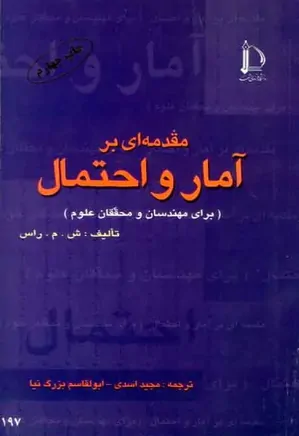
\includegraphics[keepaspectratio]{images/img_035.png}}

}

\caption{image}

\end{figure}%

\begin{figure}[H]

{\centering \pandocbounded{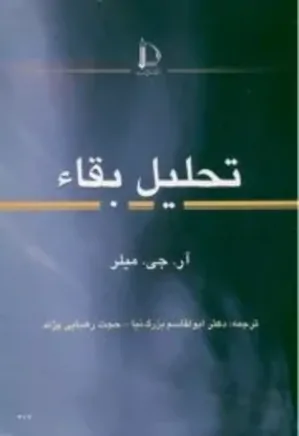
\includegraphics[keepaspectratio]{images/img_048.png}}

}

\caption{image}

\end{figure}%

\begin{figure}[H]

{\centering \pandocbounded{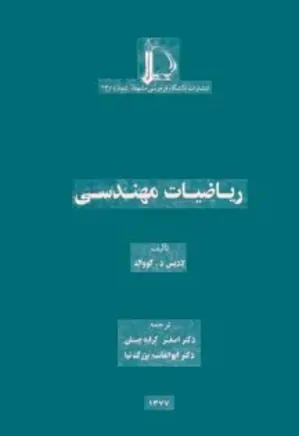
\includegraphics[keepaspectratio]{images/img_073.png}}

}

\caption{image}

\end{figure}%

\begin{figure}[H]

{\centering \pandocbounded{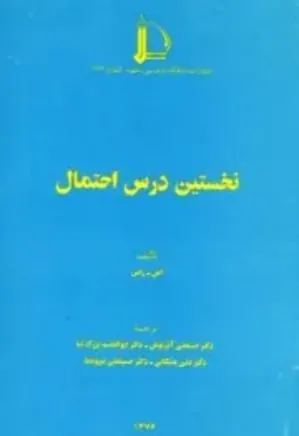
\includegraphics[keepaspectratio]{images/img_092.png}}

}

\caption{image}

\end{figure}%

\begin{figure}[H]

{\centering \pandocbounded{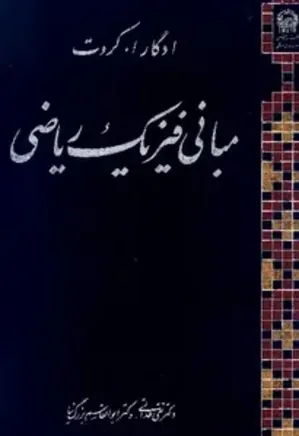
\includegraphics[keepaspectratio]{images/img_102.png}}

}

\caption{image}

\end{figure}%

\begin{figure}[H]

{\centering \pandocbounded{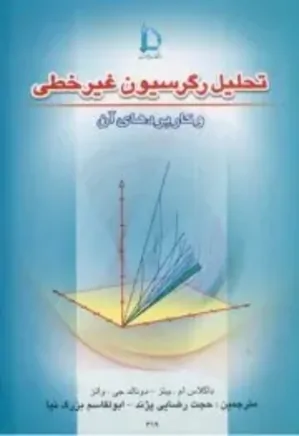
\includegraphics[keepaspectratio]{images/img_112.png}}

}

\caption{image}

\end{figure}%

\begin{figure}[H]

{\centering \pandocbounded{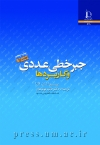
\includegraphics[keepaspectratio]{images/img_049.jpg}}

}

\caption{image}

\end{figure}%

\begin{figure}[H]

{\centering \pandocbounded{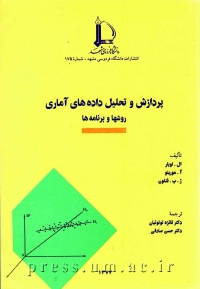
\includegraphics[keepaspectratio]{images/img_068.jpg}}

}

\caption{image}

\end{figure}%

\begin{figure}[H]

{\centering \pandocbounded{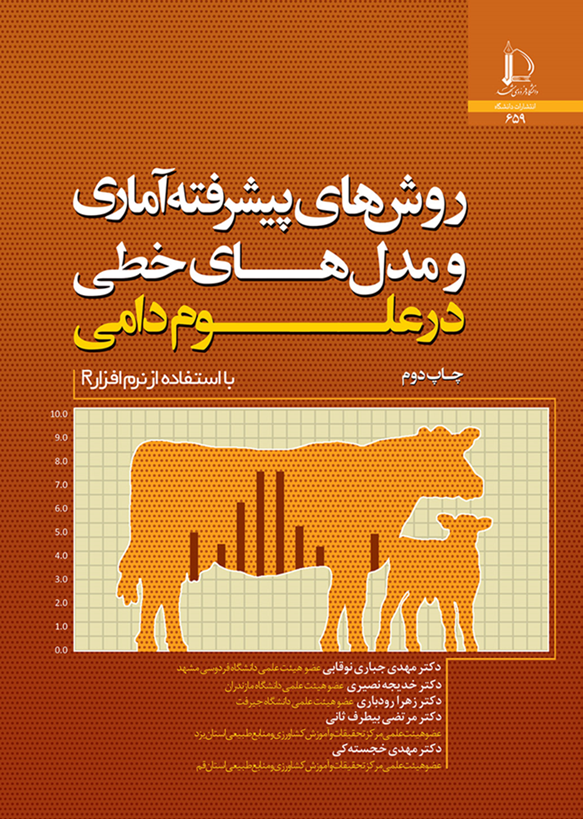
\includegraphics[keepaspectratio]{images/img_000.png}}

}

\caption{image}

\end{figure}%

\begin{figure}[H]

{\centering \pandocbounded{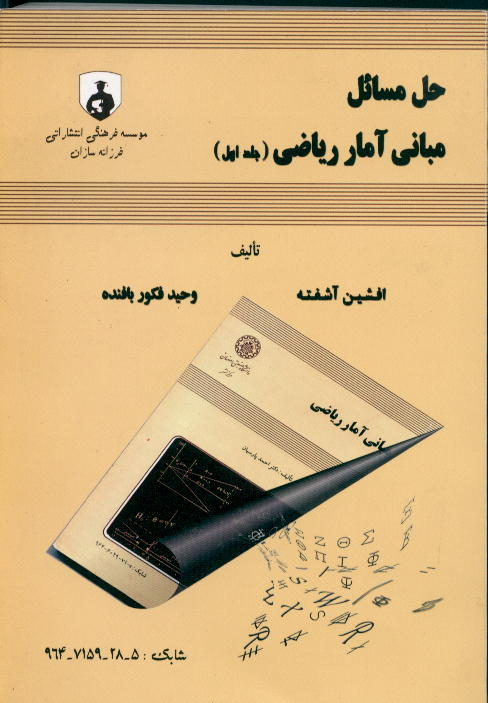
\includegraphics[keepaspectratio]{images/img_014.jpg}}

}

\caption{image}

\end{figure}%

\begin{figure}[H]

{\centering \pandocbounded{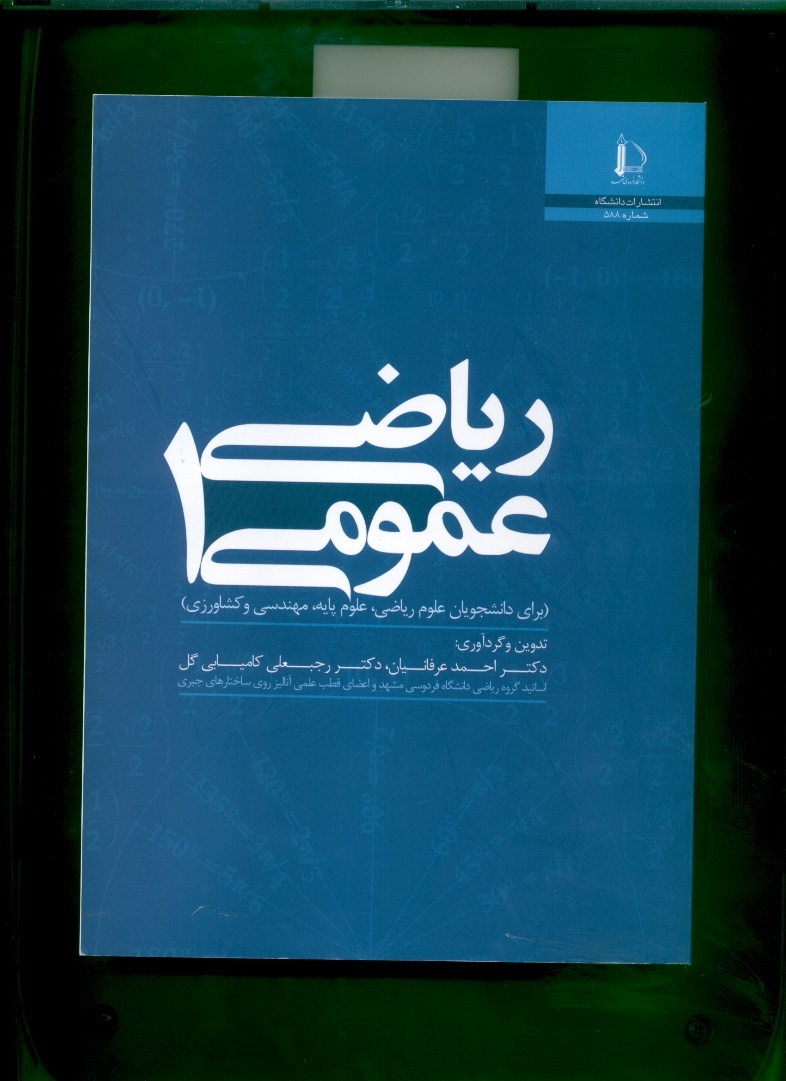
\includegraphics[keepaspectratio]{images/img_026.jpeg}}

}

\caption{image}

\end{figure}%

\begin{figure}[H]

{\centering \pandocbounded{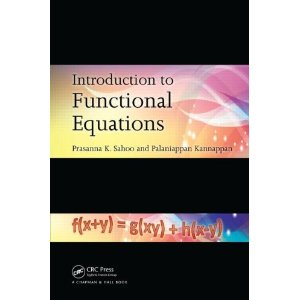
\includegraphics[keepaspectratio]{images/img_039.jpg}}

}

\caption{image}

\end{figure}%

\begin{figure}[H]

{\centering \pandocbounded{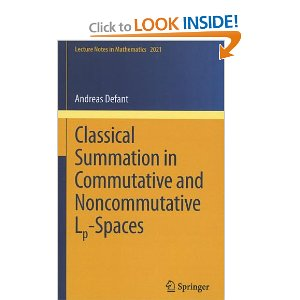
\includegraphics[keepaspectratio]{images/img_065.jpg}}

}

\caption{image}

\end{figure}%

\begin{figure}[H]

{\centering \pandocbounded{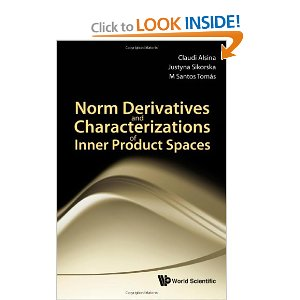
\includegraphics[keepaspectratio]{images/img_084.jpg}}

}

\caption{image}

\end{figure}%

\begin{figure}[H]

{\centering \pandocbounded{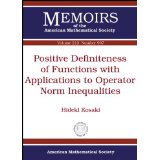
\includegraphics[keepaspectratio]{images/img_097.jpg}}

}

\caption{image}

\end{figure}%

\begin{figure}[H]

{\centering \pandocbounded{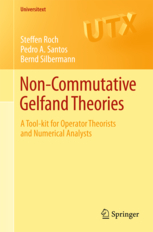
\includegraphics[keepaspectratio]{images/img_107.jpg}}

}

\caption{image}

\end{figure}%

۱۰

\begin{figure}[H]

{\centering \pandocbounded{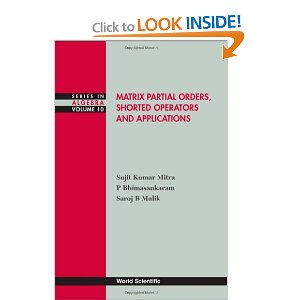
\includegraphics[keepaspectratio]{images/img_040.jpg}}

}

\caption{image}

\end{figure}%

\begin{figure}[H]

{\centering \pandocbounded{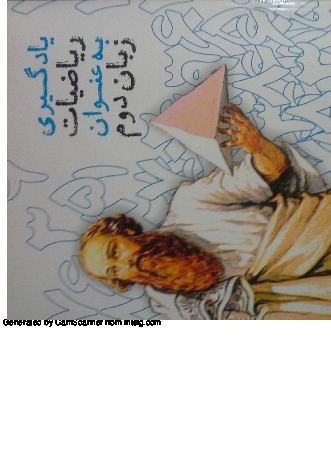
\includegraphics[keepaspectratio]{images/img_059.jpg}}

}

\caption{image}

\end{figure}%

\begin{figure}[H]

{\centering \pandocbounded{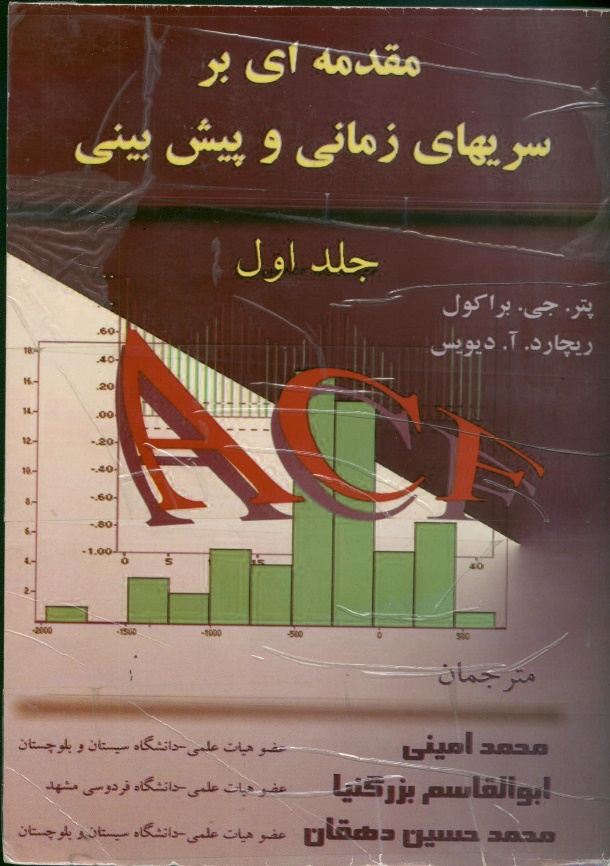
\includegraphics[keepaspectratio]{images/img_078.jpeg}}

}

\caption{image}

\end{figure}%

\begin{figure}[H]

{\centering \pandocbounded{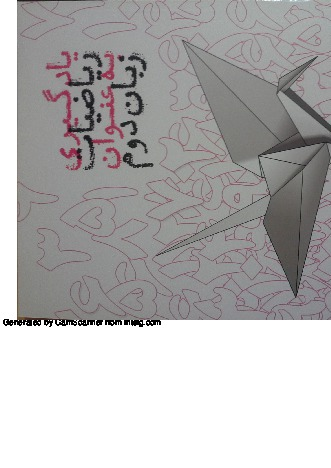
\includegraphics[keepaspectratio]{images/img_009.jpg}}

}

\caption{image}

\end{figure}%

\begin{figure}[H]

{\centering \pandocbounded{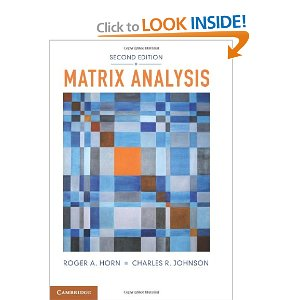
\includegraphics[keepaspectratio]{images/img_021.jpg}}

}

\caption{image}

\end{figure}%

\begin{figure}[H]

{\centering \pandocbounded{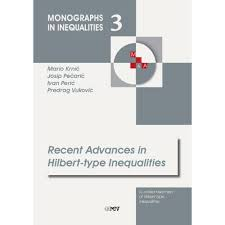
\includegraphics[keepaspectratio]{images/img_030.jpg}}

}

\caption{image}

\end{figure}%

\begin{figure}[H]

{\centering \pandocbounded{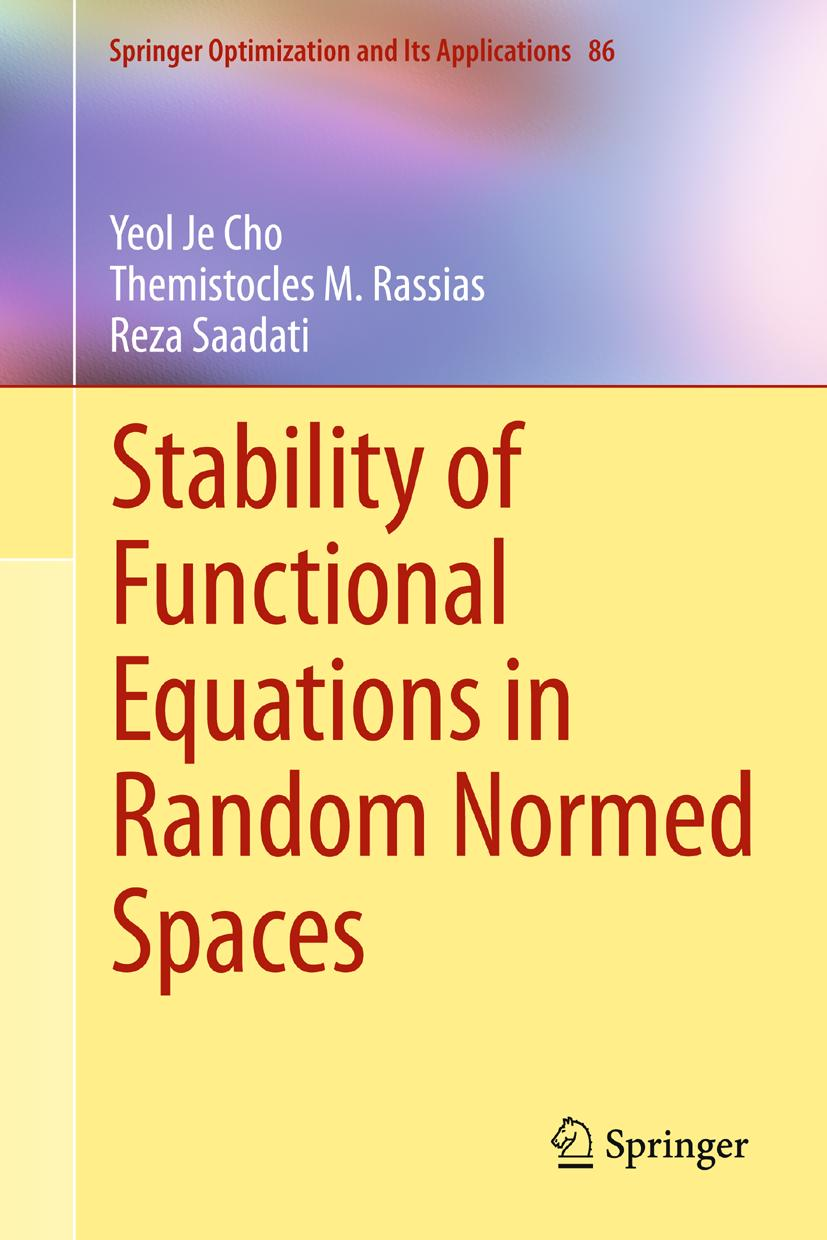
\includegraphics[keepaspectratio]{images/img_050.jpg}}

}

\caption{image}

\end{figure}%

\begin{figure}[H]

{\centering \pandocbounded{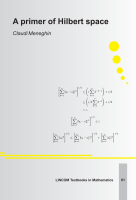
\includegraphics[keepaspectratio]{images/img_074.png}}

}

\caption{image}

\end{figure}%

\begin{figure}[H]

{\centering \pandocbounded{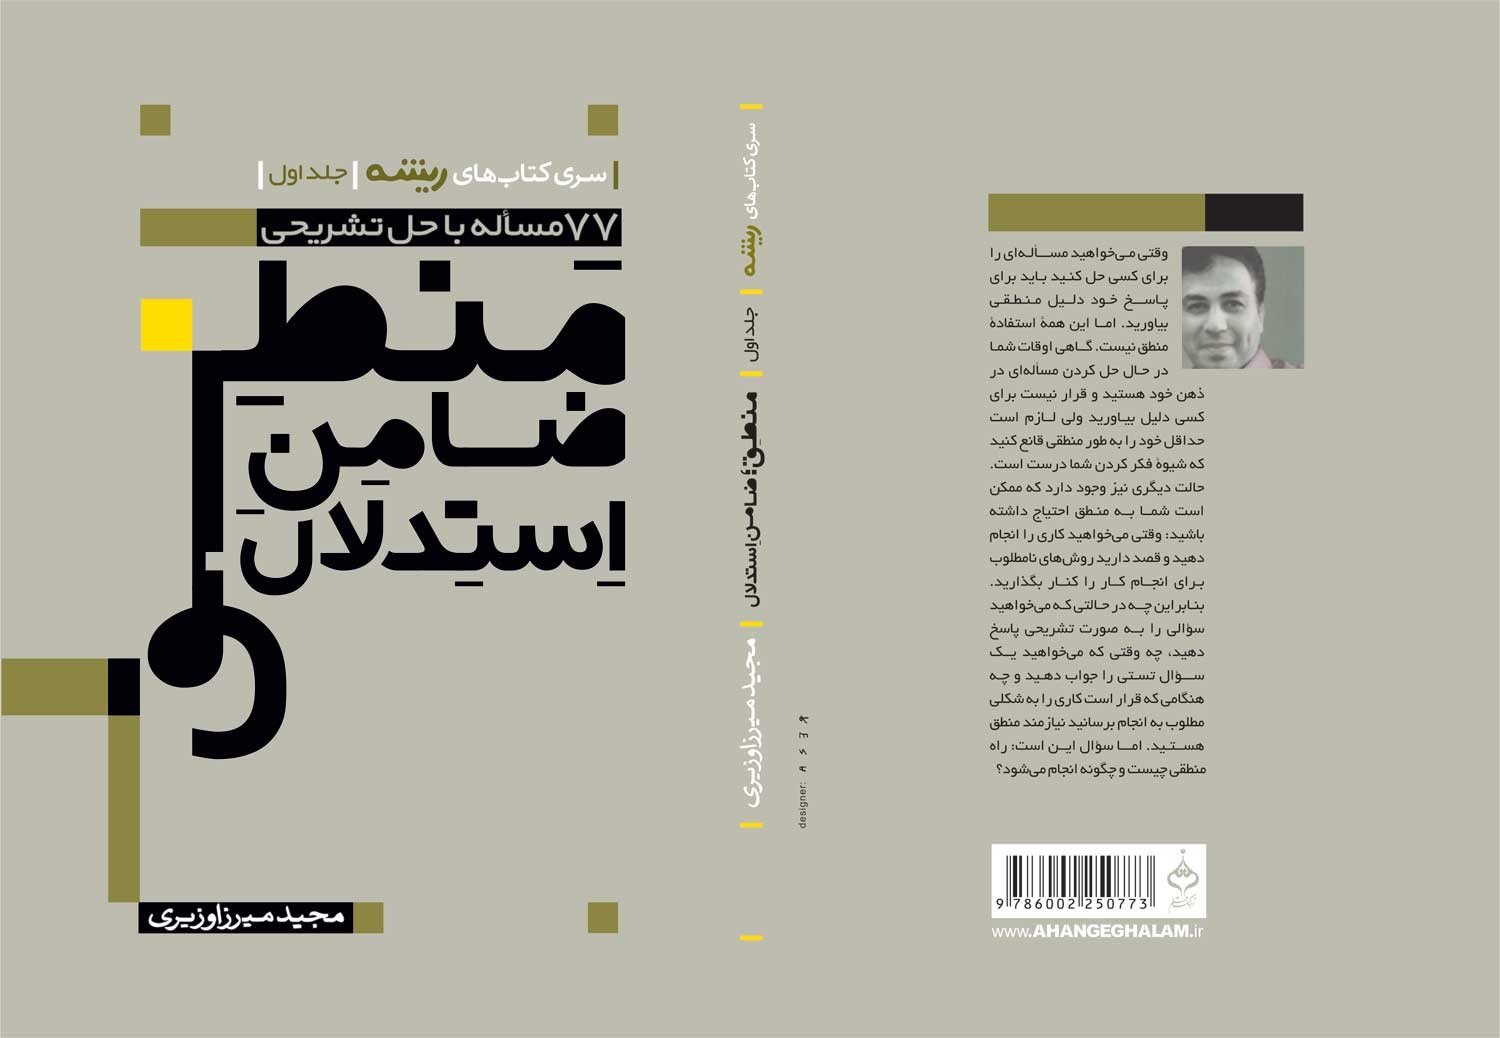
\includegraphics[keepaspectratio]{images/img_093.jpg}}

}

\caption{image}

\end{figure}%

\begin{figure}[H]

{\centering \pandocbounded{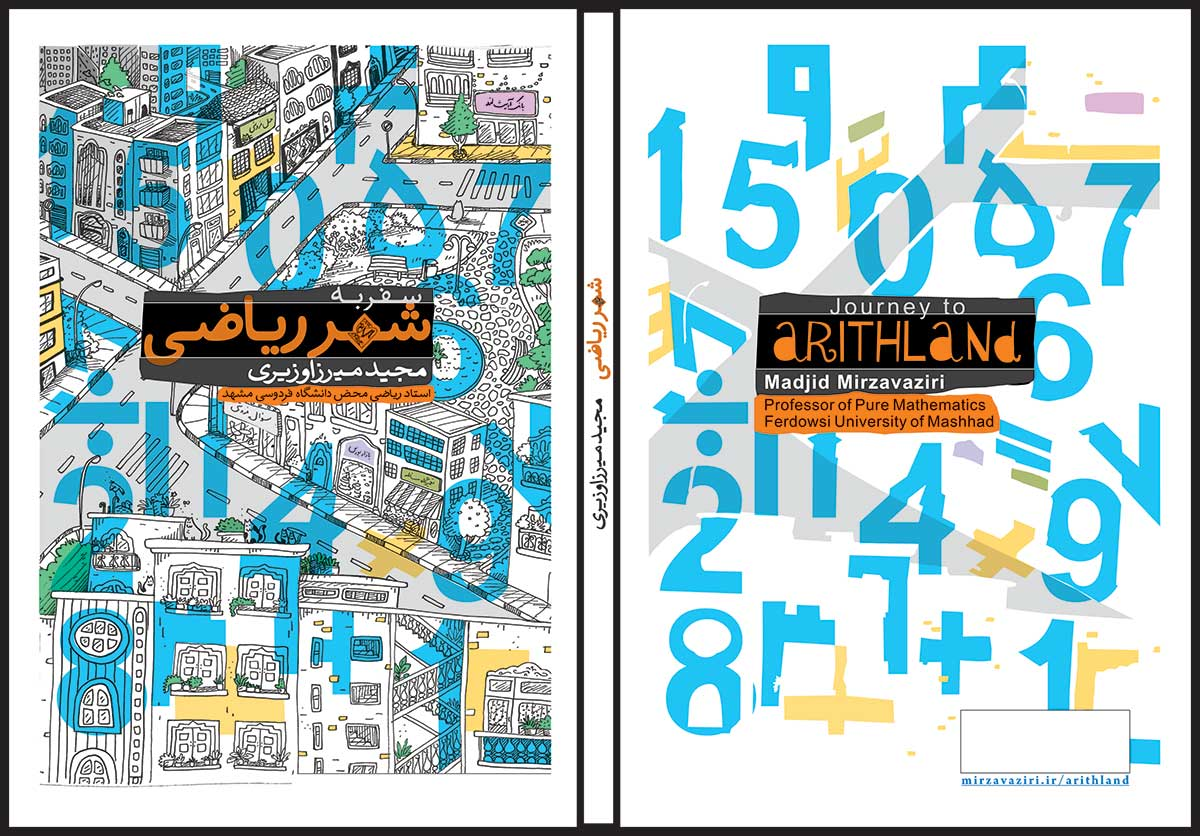
\includegraphics[keepaspectratio]{images/img_103.jpg}}

}

\caption{image}

\end{figure}%

\begin{figure}[H]

{\centering \pandocbounded{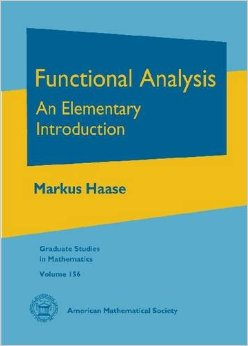
\includegraphics[keepaspectratio]{images/img_031.jpg}}

}

\caption{image}

\end{figure}%

\begin{figure}[H]

{\centering \pandocbounded{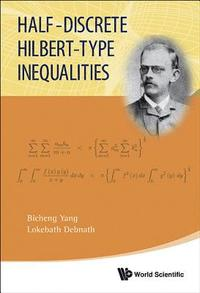
\includegraphics[keepaspectratio]{images/img_051.jpg}}

}

\caption{image}

\end{figure}%

\begin{figure}[H]

{\centering \pandocbounded{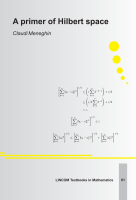
\includegraphics[keepaspectratio]{images/img_074.png}}

}

\caption{image}

\end{figure}%

\begin{figure}[H]

{\centering \pandocbounded{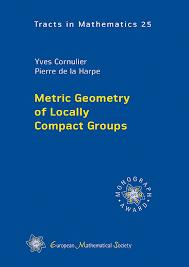
\includegraphics[keepaspectratio]{images/img_069.jpg}}

}

\caption{image}

\end{figure}%

\begin{figure}[H]

{\centering \pandocbounded{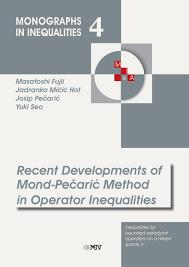
\includegraphics[keepaspectratio]{images/img_003.jpg}}

}

\caption{image}

\end{figure}%

\begin{figure}[H]

{\centering \pandocbounded{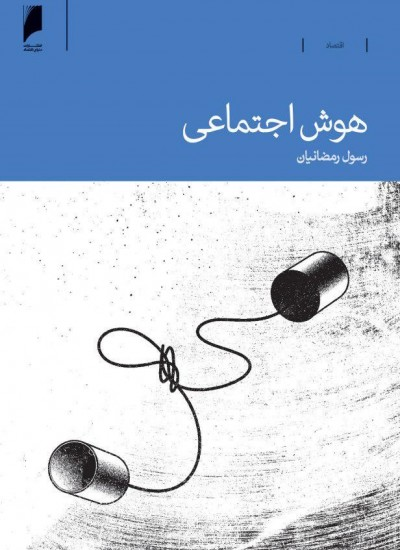
\includegraphics[keepaspectratio]{images/img_015.jpg}}

}

\caption{image}

\end{figure}%

\begin{figure}[H]

{\centering \pandocbounded{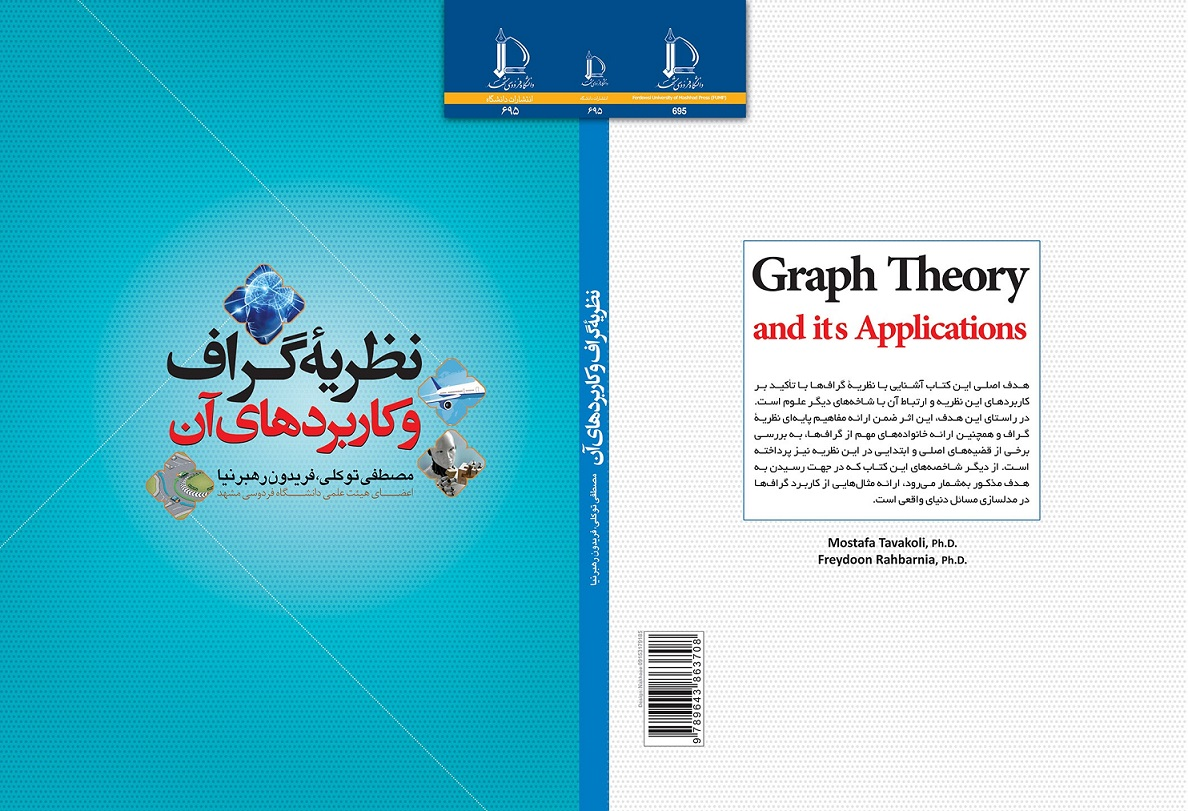
\includegraphics[keepaspectratio]{images/img_024.jpg}}

}

\caption{image}

\end{figure}%

۱۰

\begin{figure}[H]

{\centering \pandocbounded{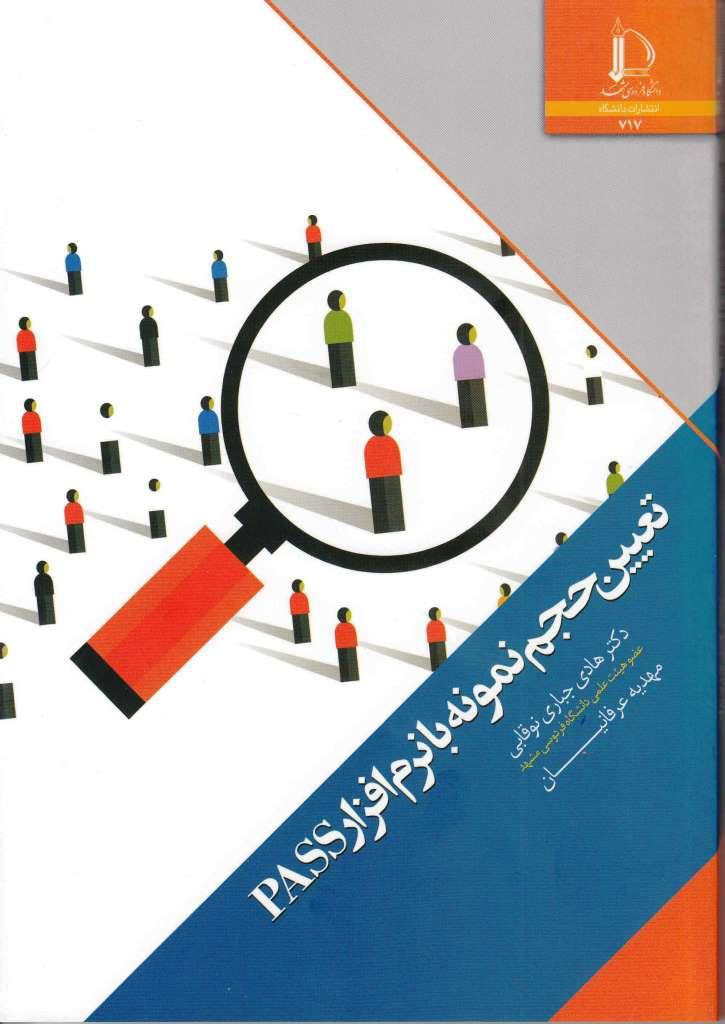
\includegraphics[keepaspectratio]{images/img_041.jpg}}

}

\caption{image}

\end{figure}%

\begin{figure}[H]

{\centering \pandocbounded{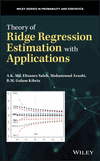
\includegraphics[keepaspectratio]{images/img_066.png}}

}

\caption{image}

\end{figure}%

\begin{figure}[H]

{\centering \pandocbounded{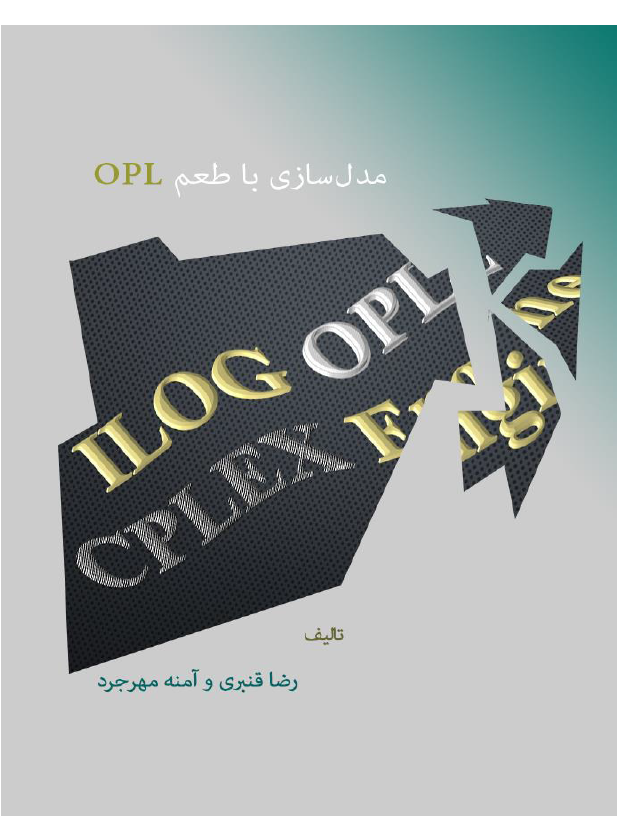
\includegraphics[keepaspectratio]{images/img_085.png}}

}

\caption{image}

\end{figure}%

\begin{figure}[H]

{\centering \pandocbounded{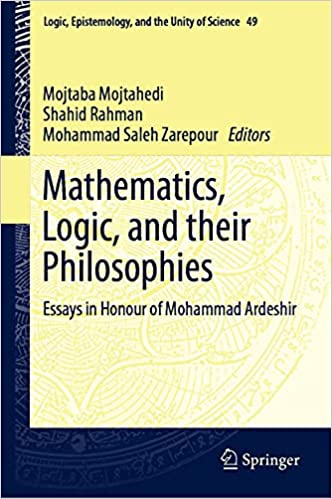
\includegraphics[keepaspectratio]{images/img_098.jpg}}

}

\caption{image}

\end{figure}%

\begin{figure}[H]

{\centering \pandocbounded{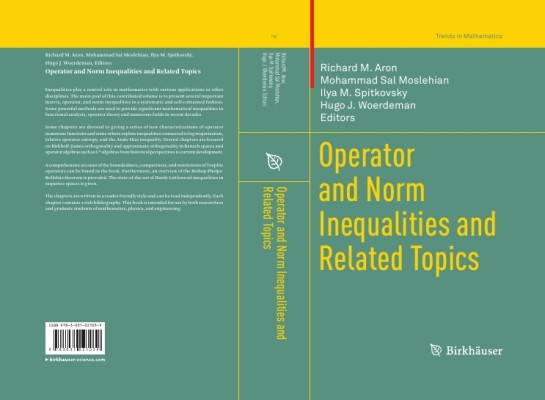
\includegraphics[keepaspectratio]{images/img_110.jpg}}

}

\caption{image}

\end{figure}%

\begin{figure}[H]

{\centering \pandocbounded{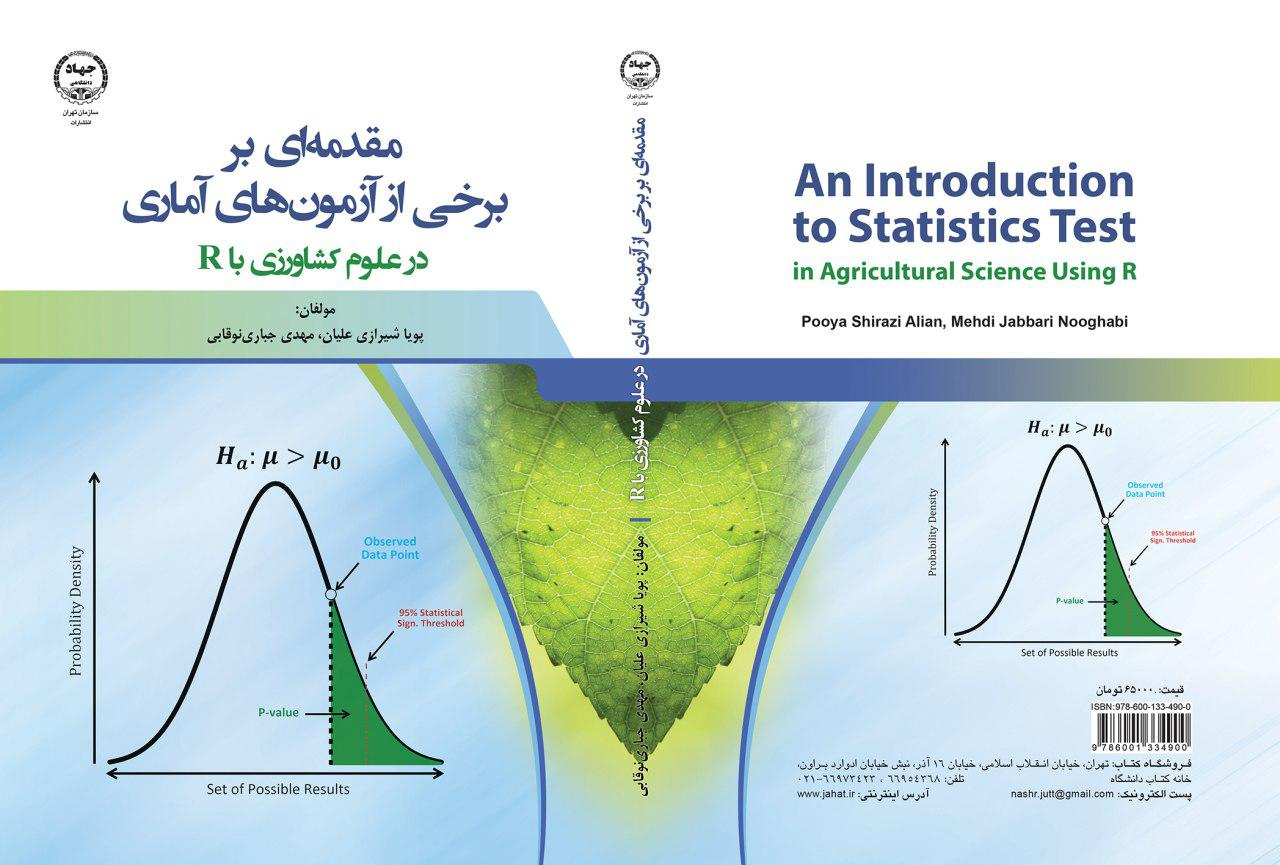
\includegraphics[keepaspectratio]{images/img_042.jpg}}

}

\caption{image}

\end{figure}%

\begin{figure}[H]

{\centering \pandocbounded{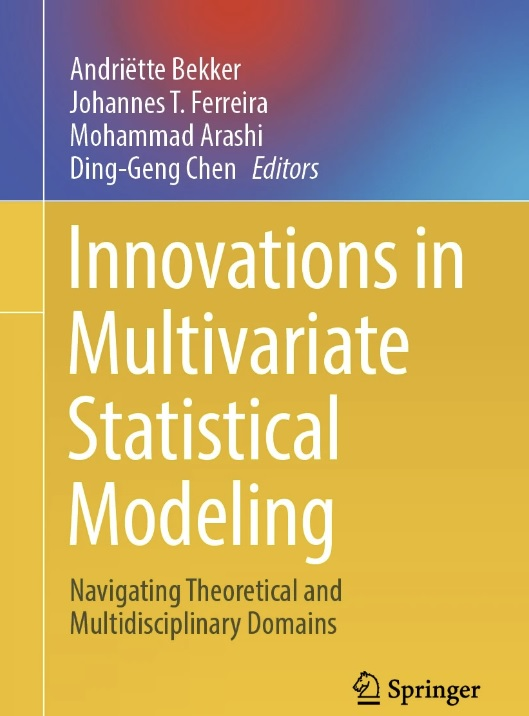
\includegraphics[keepaspectratio]{images/img_060.jpg}}

}

\caption{image}

\end{figure}%

\begin{figure}[H]

{\centering \pandocbounded{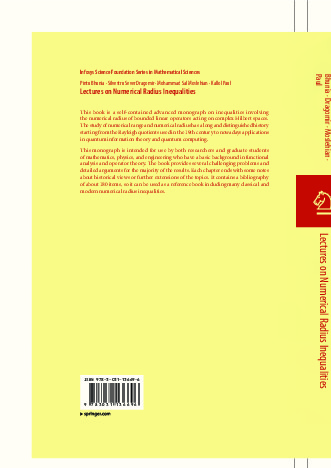
\includegraphics[keepaspectratio]{images/img_086.jpg}}

}

\caption{image}

\end{figure}%

\begin{figure}[H]

{\centering \pandocbounded{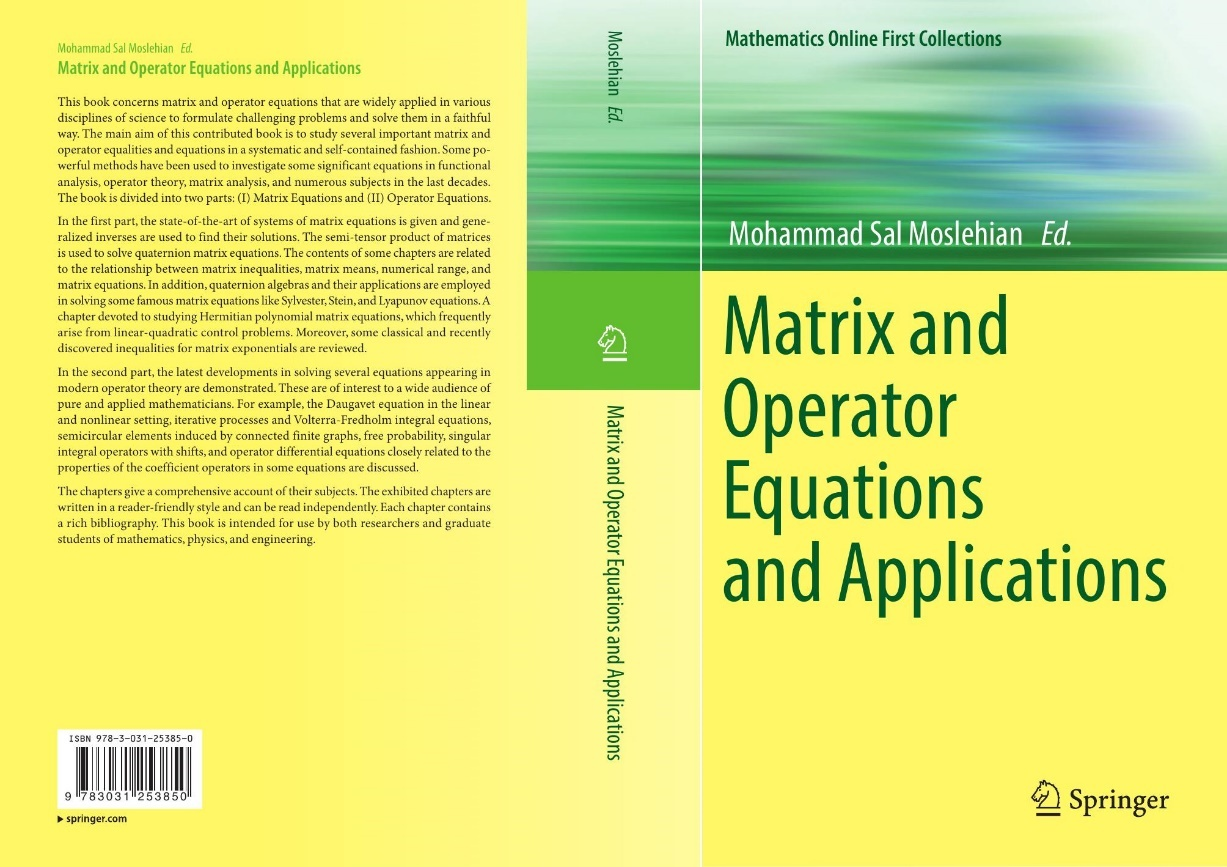
\includegraphics[keepaspectratio]{images/img_010.jpeg}}

}

\caption{image}

\end{figure}%

\begin{figure}[H]

{\centering \pandocbounded{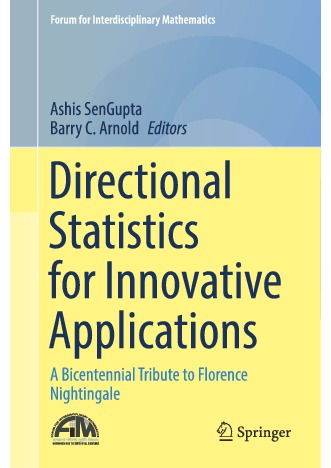
\includegraphics[keepaspectratio]{images/img_017.jpg}}

}

\caption{image}

\end{figure}%

\begin{figure}[H]

{\centering \pandocbounded{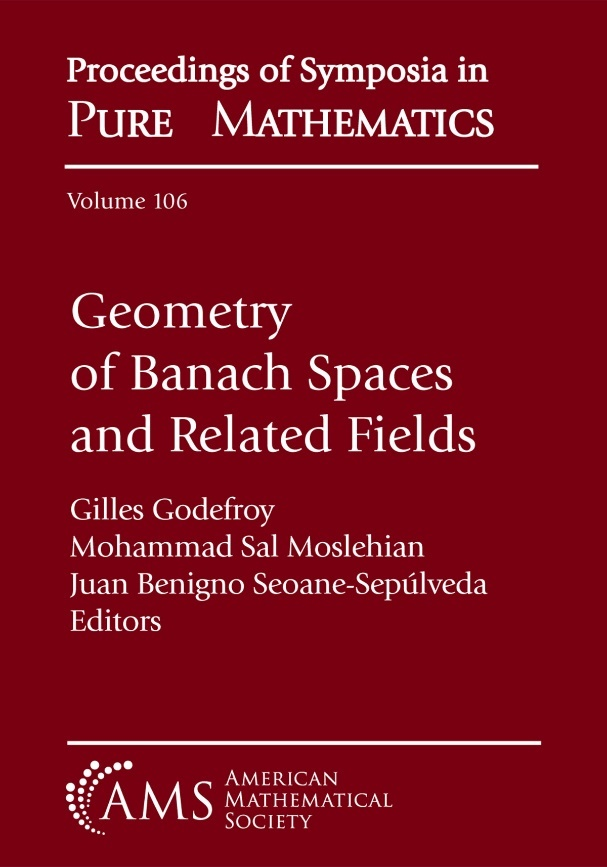
\includegraphics[keepaspectratio]{images/img_032.jpeg}}

}

\caption{image}

\end{figure}%

\begin{figure}[H]

{\centering \pandocbounded{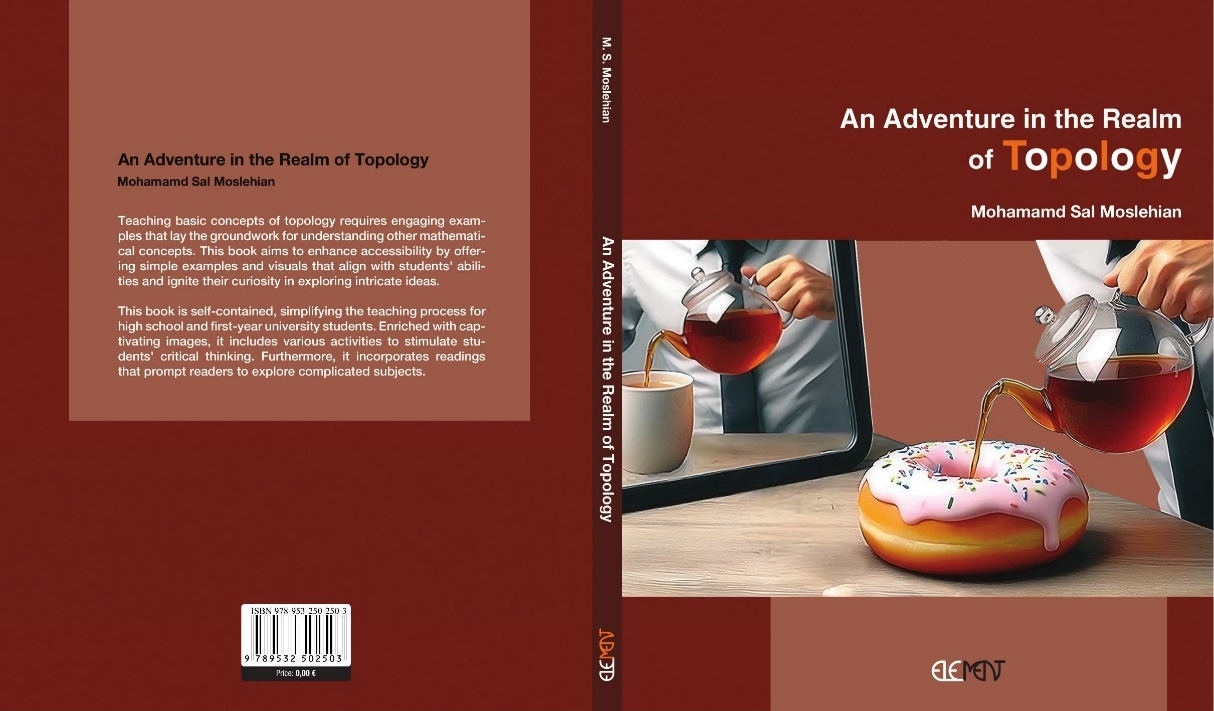
\includegraphics[keepaspectratio]{images/img_055.jpeg}}

}

\caption{image}

\end{figure}%

\begin{figure}[H]

{\centering \pandocbounded{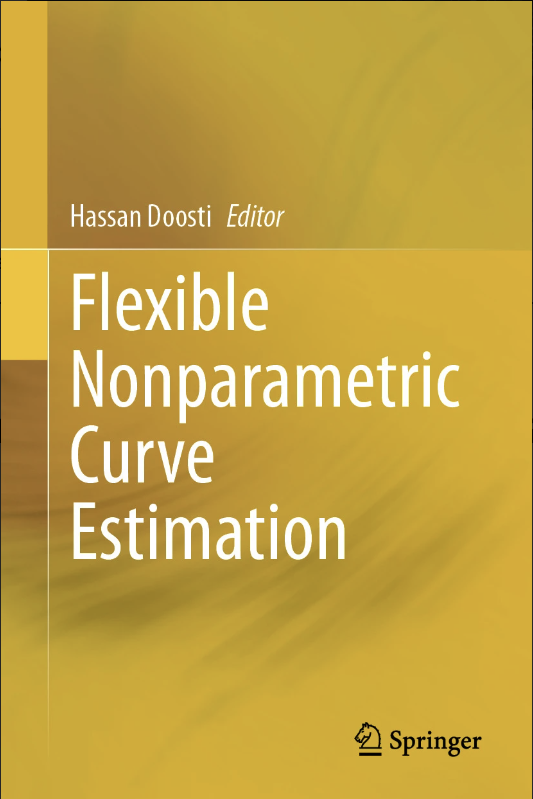
\includegraphics[keepaspectratio]{images/img_075.png}}

}

\caption{image}

\end{figure}%

\begin{figure}[H]

{\centering \pandocbounded{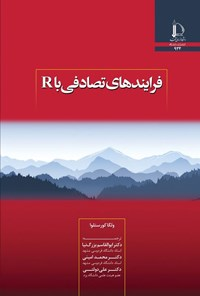
\includegraphics[keepaspectratio]{images/img_094.jpg}}

}

\caption{image}

\end{figure}%

\begin{figure}[H]

{\centering \pandocbounded{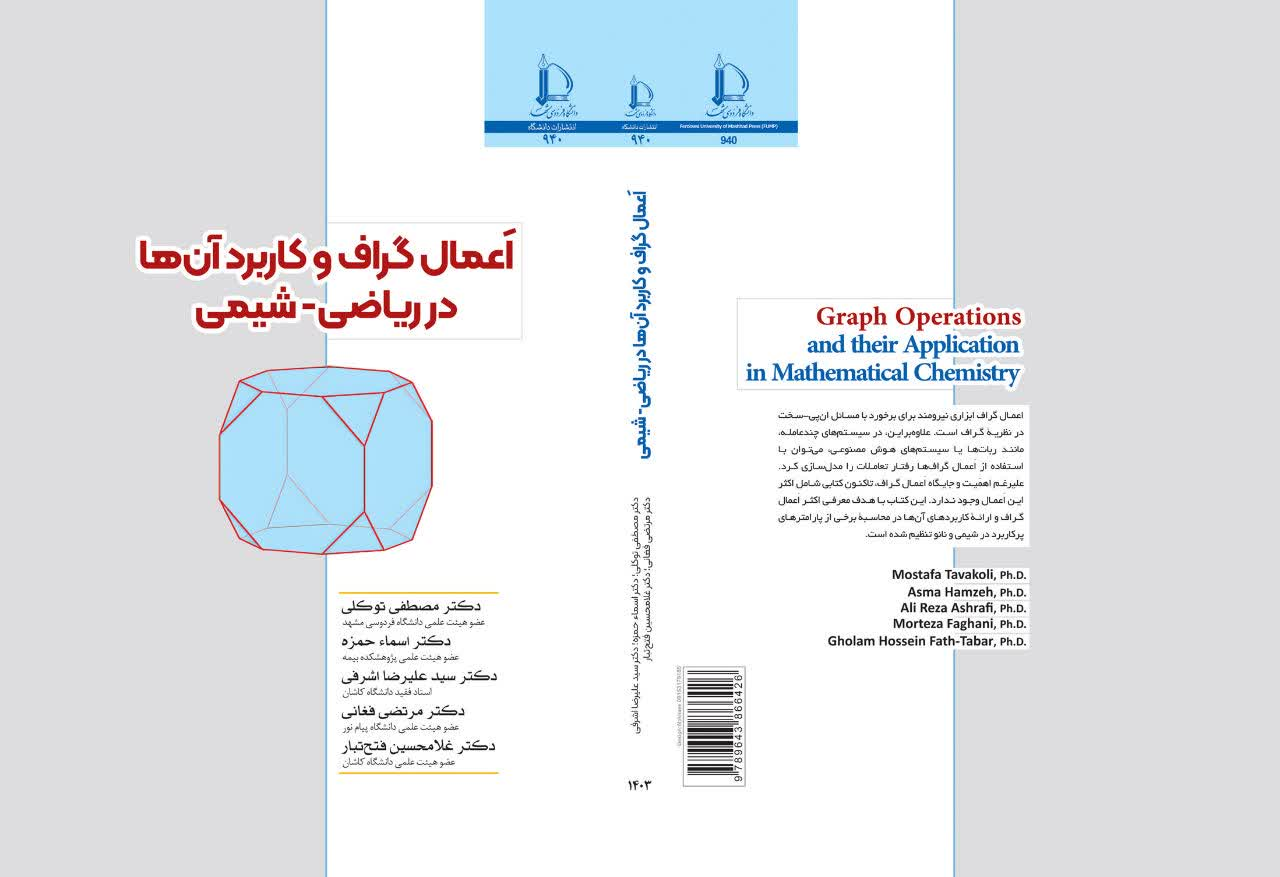
\includegraphics[keepaspectratio]{images/img_105.jpg}}

}

\caption{image}

\end{figure}%

\begin{figure}[H]

{\centering \pandocbounded{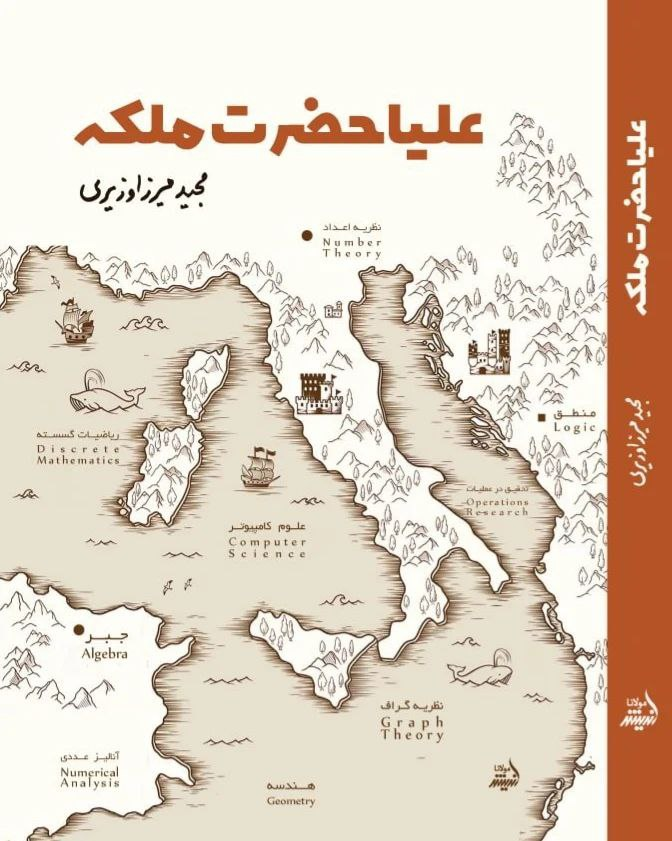
\includegraphics[keepaspectratio]{images/img_033.jpg}}

}

\caption{image}

\end{figure}%

\begin{figure}[H]

{\centering \pandocbounded{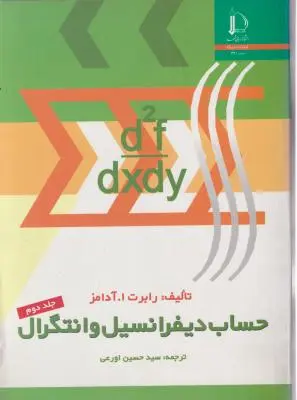
\includegraphics[keepaspectratio]{images/img_052.png}}

}

\caption{image}

\end{figure}%

\begin{figure}[H]

{\centering \pandocbounded{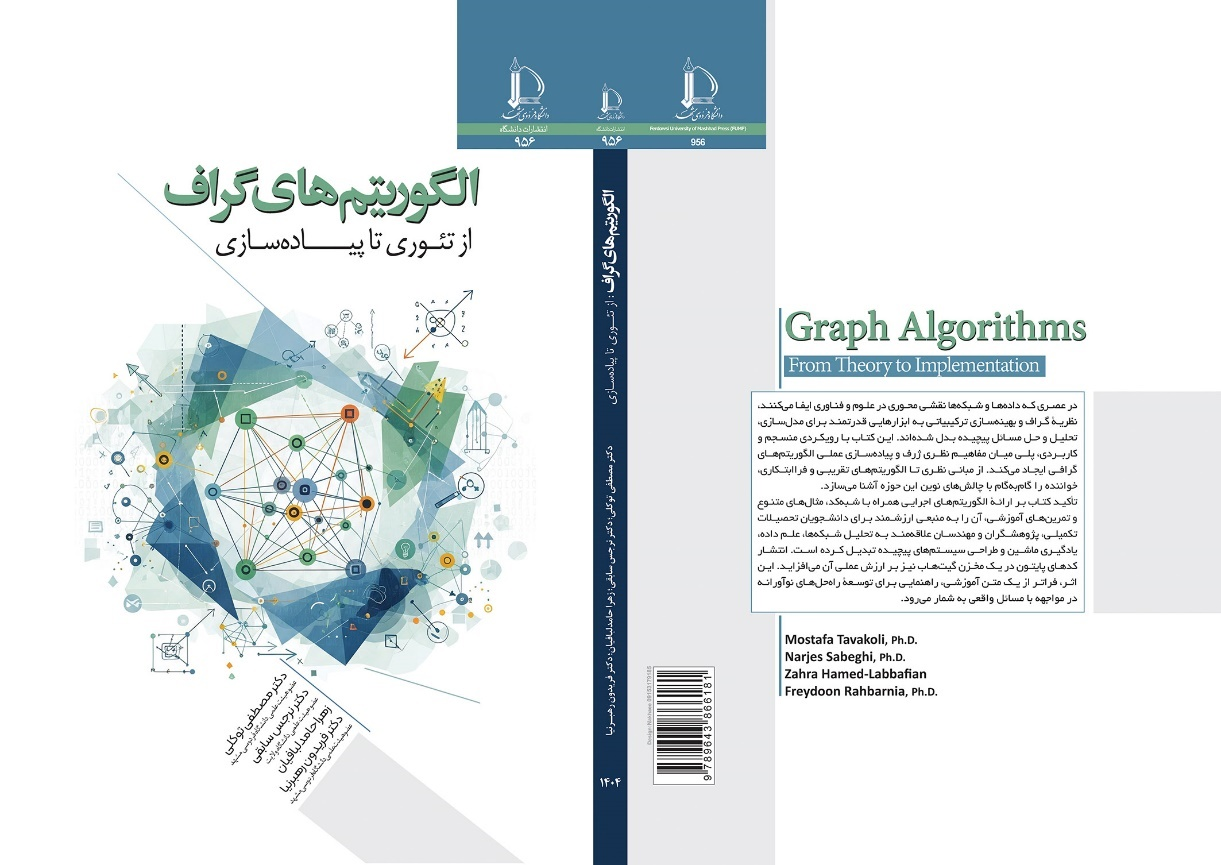
\includegraphics[keepaspectratio]{images/img_070.jpeg}}

}

\caption{image}

\end{figure}%

\begin{figure}[H]

{\centering \pandocbounded{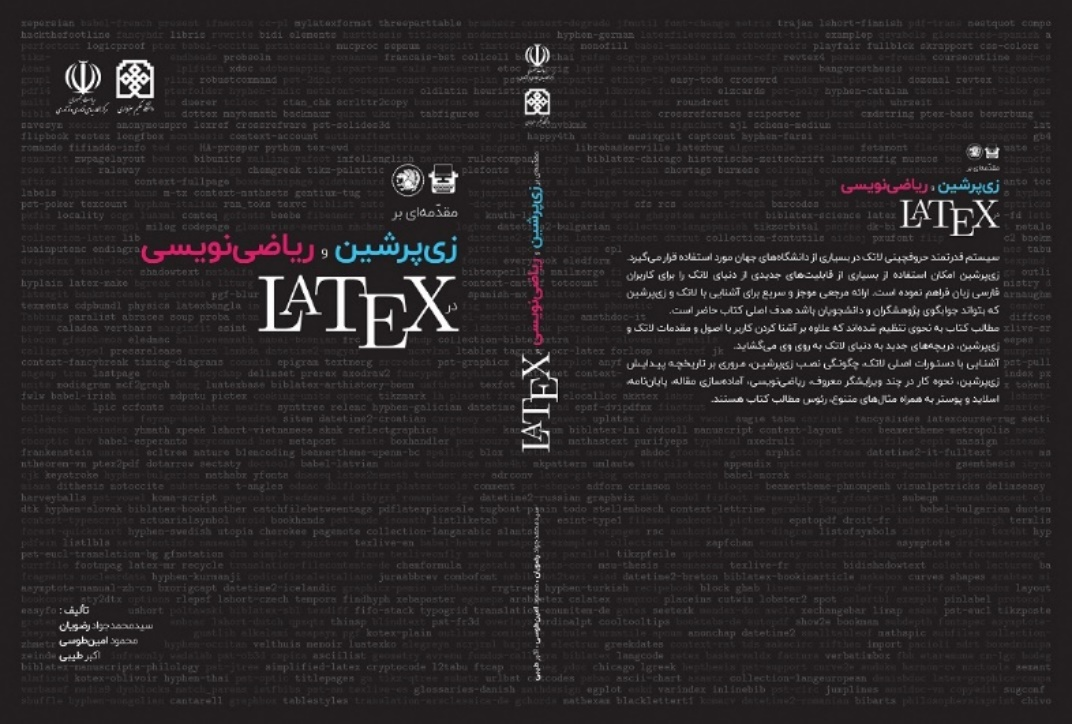
\includegraphics[keepaspectratio]{images/img_004.jpeg}}

}

\caption{image}

\end{figure}%

\begin{figure}[H]

{\centering \pandocbounded{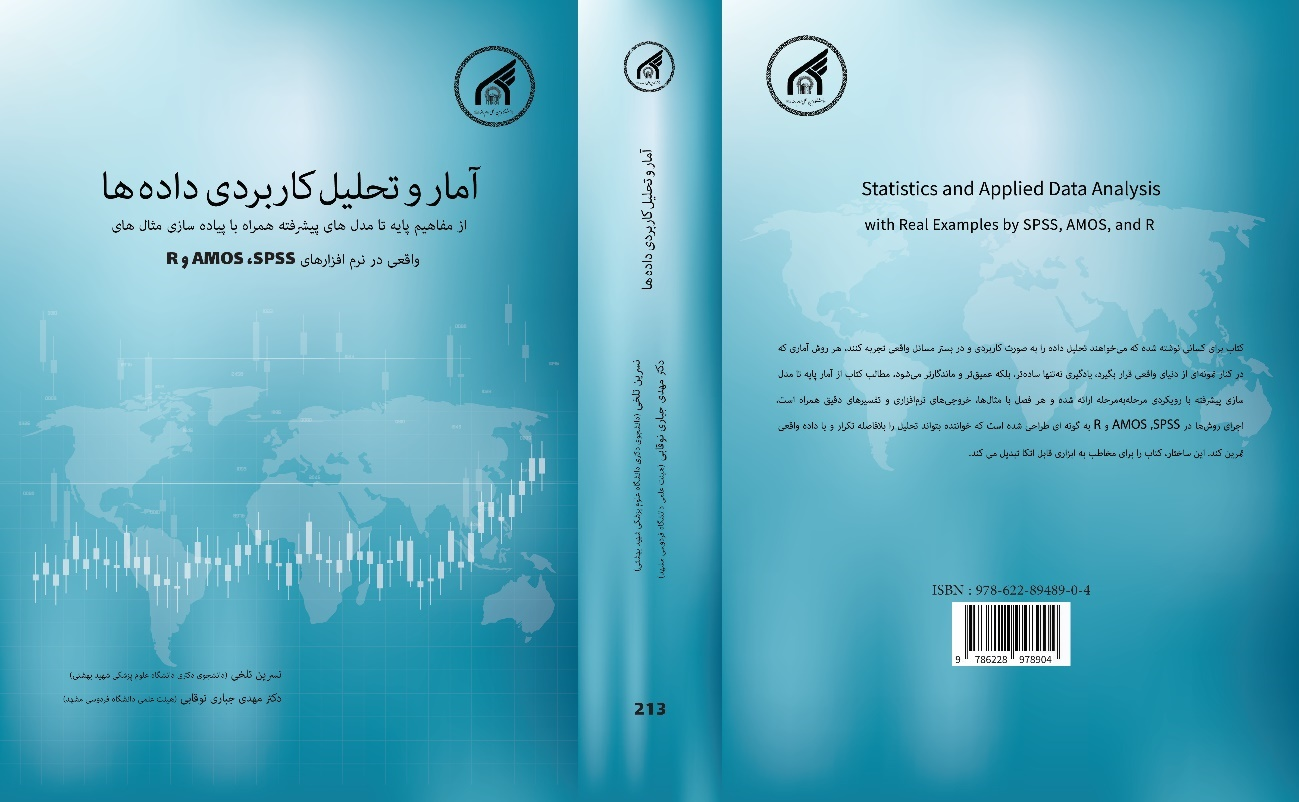
\includegraphics[keepaspectratio]{images/img_012.jpeg}}

}

\caption{image}

\end{figure}%

\begin{figure}[H]

{\centering \pandocbounded{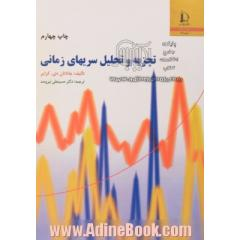
\includegraphics[keepaspectratio]{images/img_025.jpg}}

}

\caption{image}

\end{figure}%

\begin{figure}[H]

{\centering \pandocbounded{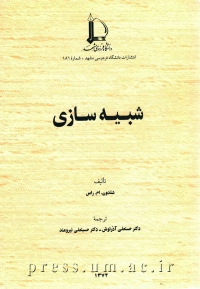
\includegraphics[keepaspectratio]{images/img_046.jpg}}

}

\caption{image}

\end{figure}%

\begin{figure}[H]

{\centering \pandocbounded{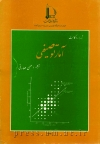
\includegraphics[keepaspectratio]{images/img_067.jpg}}

}

\caption{image}

\end{figure}%

\begin{figure}[H]

{\centering \pandocbounded{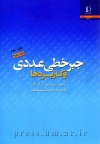
\includegraphics[keepaspectratio]{images/img_087.jpg}}

}

\caption{image}

\end{figure}%

\begin{figure}[H]

{\centering \pandocbounded{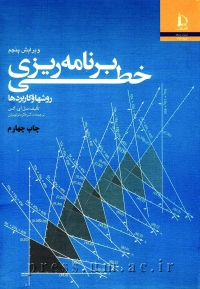
\includegraphics[keepaspectratio]{images/img_100.jpg}}

}

\caption{image}

\end{figure}%

\begin{figure}[H]

{\centering \pandocbounded{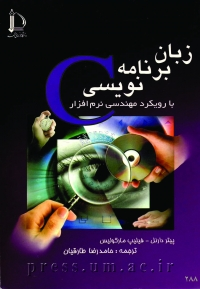
\includegraphics[keepaspectratio]{images/img_111.jpg}}

}

\caption{image}

\end{figure}%

\begin{figure}[H]

{\centering \pandocbounded{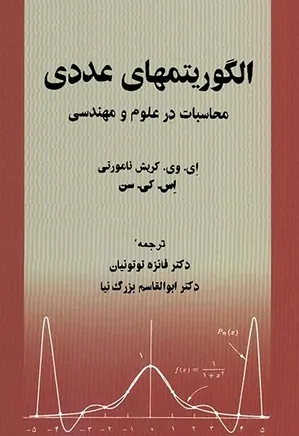
\includegraphics[keepaspectratio]{images/img_043.png}}

}

\caption{image}

\end{figure}%

\begin{figure}[H]

{\centering \pandocbounded{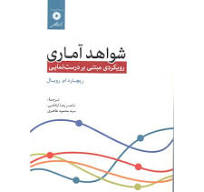
\includegraphics[keepaspectratio]{images/img_061.jpg}}

}

\caption{image}

\end{figure}%

\begin{figure}[H]

{\centering \pandocbounded{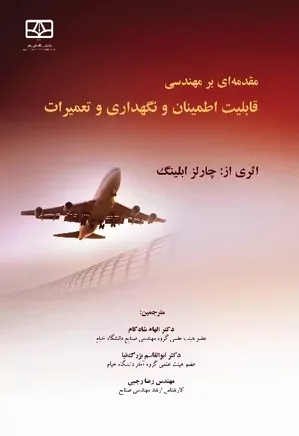
\includegraphics[keepaspectratio]{images/img_088.png}}

}

\caption{image}

\end{figure}%

\begin{figure}[H]

{\centering \pandocbounded{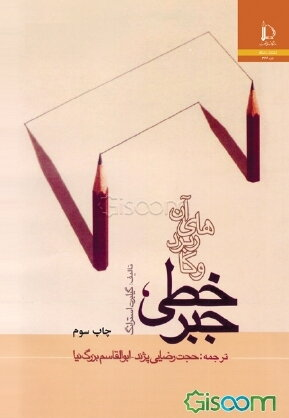
\includegraphics[keepaspectratio]{images/img_005.jpg}}

}

\caption{image}

\end{figure}%

\begin{figure}[H]

{\centering \pandocbounded{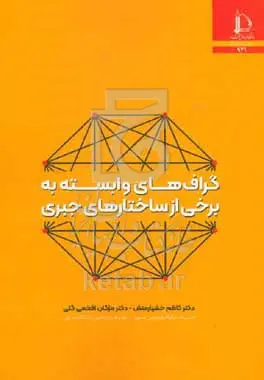
\includegraphics[keepaspectratio]{images/img_018.png}}

}

\caption{image}

\end{figure}%

\bookmarksetup{startatroot}

\chapter{ضمایم}\label{ux636ux645ux627ux6ccux645}

\bookmarksetup{startatroot}

\chapter{ضمایم}\label{ux636ux645ux627ux6ccux645-1}

\section{شهدای
دانشکده}\label{ux634ux647ux62fux627ux6cc-ux62fux627ux646ux634ux6a9ux62fux647}

\section{آمار دانشجویان بین الملل
جاری}\label{ux622ux645ux627ux631-ux62fux627ux646ux634ux62cux648ux6ccux627ux646-ux628ux6ccux646-ux627ux644ux645ux644ux644-ux62cux627ux631ux6cc}

\hspace{0pt}

{\def\LTcaptype{none} % do not increment counter
\begin{longtable}[]{@{}
  >{\raggedright\arraybackslash}p{(\linewidth - 18\tabcolsep) * \real{0.1000}}
  >{\raggedright\arraybackslash}p{(\linewidth - 18\tabcolsep) * \real{0.1000}}
  >{\raggedright\arraybackslash}p{(\linewidth - 18\tabcolsep) * \real{0.1000}}
  >{\raggedright\arraybackslash}p{(\linewidth - 18\tabcolsep) * \real{0.1000}}
  >{\raggedright\arraybackslash}p{(\linewidth - 18\tabcolsep) * \real{0.1000}}
  >{\raggedright\arraybackslash}p{(\linewidth - 18\tabcolsep) * \real{0.1000}}
  >{\raggedright\arraybackslash}p{(\linewidth - 18\tabcolsep) * \real{0.1000}}
  >{\raggedright\arraybackslash}p{(\linewidth - 18\tabcolsep) * \real{0.1000}}
  >{\raggedright\arraybackslash}p{(\linewidth - 18\tabcolsep) * \real{0.1000}}
  >{\raggedright\arraybackslash}p{(\linewidth - 18\tabcolsep) * \real{0.1000}}@{}}
\toprule\noalign{}
\begin{minipage}[b]{\linewidth}\raggedright
ردیف
\end{minipage} & \begin{minipage}[b]{\linewidth}\raggedright
رشته
\end{minipage} & \begin{minipage}[b]{\linewidth}\raggedright
مقطع
\end{minipage} & \begin{minipage}[b]{\linewidth}\raggedright
روزانه
\end{minipage} & \begin{minipage}[b]{\linewidth}\raggedright
روزانه
\end{minipage} & \begin{minipage}[b]{\linewidth}\raggedright
روزانه
\end{minipage} & \begin{minipage}[b]{\linewidth}\raggedright
نوبت دوم
\end{minipage} & \begin{minipage}[b]{\linewidth}\raggedright
نوبت دوم
\end{minipage} & \begin{minipage}[b]{\linewidth}\raggedright
نوبت دوم
\end{minipage} & \begin{minipage}[b]{\linewidth}\raggedright
جمع کل
\end{minipage} \\
\midrule\noalign{}
\endhead
\bottomrule\noalign{}
\endlastfoot
& & & زن & مرد & جمع & زن & مرد & جمع & \\
۱ & آموزش ریاضی & کارشناسی ارشد & ۱ & ۰ & ۱ & ۰ & ۰ & ۰ & ۱ \\
۲ & ریاضی محض گرایش آنالیز & دکتری & ۱ & ۰ & ۱ & ۰ & ۰ & ۰ & ۱ \\
۳ & آمار & کارشناسی & ۰ & ۰ & ۰ & ۲ & ۲ & ۴ & ۴ \\
۴ & آمار ریاضی & دکتری & ۰ & ۰ & ۰ & ۰ & ۱ & ۱ & ۱ \\
۵ & ریاضی کاربردی گرایش آنالیز عددی & کارشناسی ارشد & ۰ & ۰ & ۰ & ۲ & ۳
& ۵ & ۵ \\
۶ & ریاضیات و کاربردها & کارشناسی & ۰ & ۰ & ۰ & ۳ & ۲ & ۵ & ۵ \\
۷ & علوم کامپیوتر & کارشناسی & ۰ & ۰ & ۰ & ۰ & ۱ & ۱ & ۱ \\
۸ & ریاضیات و کاربردها گرایش جبر & کارشناسی ارشد & ۰ & ۰ & ۰ & ۳ & ۷ &
۱۰ & ۱۰ \\
۹ & ریاضی کاربردی گرایش تحقیق در عملیات (پژوهش محور) & دکتری & ۰ & ۰ & ۰
& ۰ & ۱ & ۱ & ۱ \\
۱۰ & ریاضیات و کاربردها گرایش آنالیز & کارشناسی ارشد & ۰ & ۰ & ۰ & ۱ & ۰
& ۱ & ۱ \\
۱۱ & ریاضیات و کاربردها گرایش گراف و ترکیبات & کارشناسی ارشد & ۰ & ۰ & ۰
& ۱ & ۰ & ۱ & ۱ \\
۱۲ & ریاضی کاربردی (پژوهش محور) & دکتری & ۰ & ۰ & ۰ & ۳ & ۱ & ۴ & ۴ \\
۱۳ & ریاضی گرایش زیر برنامه گراف و ترکیبیات & دکتری & ۰ & ۲ & ۲ & ۰ & ۰
& ۰ & ۲ \\
۱۴ & ریاضی گرایش زیر برنامه آنالیز عددی (پژوهش محور) & دکتری & ۰ & ۰ & ۰
& ۰ & ۲ & ۲ & ۲ \\
۱۵ & ریاضی کاربردی گرایش بهینه‌سازی (پژوهش محور) & دکتری & ۰ & ۰ & ۰ & ۰
& ۱ & ۱ & ۱ \\
۱۶ & ریاضی گرایش هندسه\_توپولوژی & دکتری & ۰ & ۰ & ۰ & ۰ & ۱ & ۱ & ۱ \\
۱۷ & ریاضی گرایش جبر & دکتری & ۱ & ۰ & ۱ & ۰ & ۰ & ۰ & ۱ \\
۱۸ & ریاضی گرایش آنالیز & دکتری & ۰ & ۰ & ۰ & ۱ & ۰ & ۱ & ۱ \\
جمع کل & جمع کل & جمع کل & ۳ & ۲ & ۵ & ۱۶ & ۲۲ & ۳۸ & ۴۳ \\
\end{longtable}
}

\section{آمار دانشجویان دکتری
جاری}\label{ux622ux645ux627ux631-ux62fux627ux646ux634ux62cux648ux6ccux627ux646-ux62fux6a9ux62aux631ux6cc-ux62cux627ux631ux6cc}

{\def\LTcaptype{none} % do not increment counter
\begin{longtable}[]{@{}
  >{\raggedright\arraybackslash}p{(\linewidth - 18\tabcolsep) * \real{0.1000}}
  >{\raggedright\arraybackslash}p{(\linewidth - 18\tabcolsep) * \real{0.1000}}
  >{\raggedright\arraybackslash}p{(\linewidth - 18\tabcolsep) * \real{0.1000}}
  >{\raggedright\arraybackslash}p{(\linewidth - 18\tabcolsep) * \real{0.1000}}
  >{\raggedright\arraybackslash}p{(\linewidth - 18\tabcolsep) * \real{0.1000}}
  >{\raggedright\arraybackslash}p{(\linewidth - 18\tabcolsep) * \real{0.1000}}
  >{\raggedright\arraybackslash}p{(\linewidth - 18\tabcolsep) * \real{0.1000}}
  >{\raggedright\arraybackslash}p{(\linewidth - 18\tabcolsep) * \real{0.1000}}
  >{\raggedright\arraybackslash}p{(\linewidth - 18\tabcolsep) * \real{0.1000}}
  >{\raggedright\arraybackslash}p{(\linewidth - 18\tabcolsep) * \real{0.1000}}@{}}
\toprule\noalign{}
\begin{minipage}[b]{\linewidth}\raggedright
ردیف
\end{minipage} & \begin{minipage}[b]{\linewidth}\raggedright
رشته
\end{minipage} & \begin{minipage}[b]{\linewidth}\raggedright
مقطع
\end{minipage} & \begin{minipage}[b]{\linewidth}\raggedright
روزانه
\end{minipage} & \begin{minipage}[b]{\linewidth}\raggedright
روزانه
\end{minipage} & \begin{minipage}[b]{\linewidth}\raggedright
روزانه
\end{minipage} & \begin{minipage}[b]{\linewidth}\raggedright
نوبت دوم
\end{minipage} & \begin{minipage}[b]{\linewidth}\raggedright
نوبت دوم
\end{minipage} & \begin{minipage}[b]{\linewidth}\raggedright
نوبت دوم
\end{minipage} & \begin{minipage}[b]{\linewidth}\raggedright
جمع کل
\end{minipage} \\
\midrule\noalign{}
\endhead
\bottomrule\noalign{}
\endlastfoot
& & & زن & مرد & جمع & زن & مرد & جمع & \\
۱ & ریاضی کاربردی گرایش تحقیق در عملیات & دکتری & ۱ & ۱ & ۲ & ۰ & ۰ & ۰
& ۲ \\
۲ & آموزش ریاضی & دکتری & ۳ & ۱ & ۴ & ۰ & ۰ & ۰ & ۴ \\
۳ & ریاضی محض گرایش آنالیز & دکتری & ۱ & ۰ & ۱ & ۰ & ۰ & ۰ & ۱ \\
۴ & آمار & دکتری & ۲۳ & ۵ & ۲۸ & ۰ & ۰ & ۰ & ۲۸ \\
۵ & آمار ریاضی & دکتری & ۰ & ۰ & ۰ & ۰ & ۱ & ۱ & ۱ \\
۶ & ریاضی کاربردی گرایش آنالیز عددی & دکتری & ۱ & ۲ & ۳ & ۰ & ۰ & ۰ &
۳ \\
۷ & ریاضی کاربردی زمینه آنالیز عددی & دکتری & ۱ & ۰ & ۱ & ۰ & ۰ & ۰ &
۱ \\
۸ & ریاضی محض گرایش آنالیز زمینه تابعی & دکتری & ۱ & ۰ & ۱ & ۰ & ۰ & ۰ &
۱ \\
۹ & ریاضی محض گرایش هندسه (توپولوژی) & دکتری & ۰ & ۱ & ۱ & ۰ & ۰ & ۰ &
۱ \\
۱۰ & ریاضی کاربردی گرایش تحقیق در عملیات (پژوهش محور) & دکتری & ۰ & ۰ &
۰ & ۰ & ۱ & ۱ & ۱ \\
۱۱ & ریاضی کاربردی (پژوهش محور) & دکتری & ۰ & ۰ & ۰ & ۳ & ۱ & ۴ & ۴ \\
۱۲ & ریاضی گرایش زیر برنامه گراف و ترکیبیات & دکتری & ۶ & ۶ & ۱۲ & ۱ & ۱
& ۲ & ۱۴ \\
۱۳ & ریاضی گرایش زیر برنامه آنالیز عددی & دکتری & ۱ & ۲ & ۳ & ۰ & ۰ & ۰
& ۳ \\
۱۴ & ریاضی گرایش زیر برنامه آنالیز عددی (پژوهش محور) & دکتری & ۰ & ۰ & ۰
& ۰ & ۲ & ۲ & ۲ \\
۱۵ & ریاضی کاربردی گرایش بهینه‌سازی (پژوهش محور) & دکتری & ۰ & ۰ & ۰ & ۰
& ۱ & ۱ & ۱ \\
۱۶ & ریاضی گرایش هندسه\_توپولوژی & دکتری & ۱ & ۰ & ۱ & ۰ & ۱ & ۱ & ۲ \\
۱۷ & ریاضی گرایش جبر & دکتری & ۸ & ۲ & ۱۰ & ۱ & ۱ & ۲ & ۱۲ \\
۱۸ & ریاضی گرایش آنالیز & دکتری & ۵ & ۴ & ۹ & ۱ & ۰ & ۱ & ۱۰ \\
۱۹ & ریاضی گرایش کاربردی & دکتری & ۱۳ & ۱ & ۱۴ & ۱ & ۰ & ۱ & ۱۵ \\
۲۰ & ریاضی کاربردی زمینه تحقیق در عملیات & دکتری & ۰ & ۱ & ۱ & ۰ & ۰ & ۰
& ۱ \\
جمع کل دکتری & جمع کل دکتری & جمع کل دکتری & ۶۵ & ۲۶ & ۹۱ & ۷ & ۹ & ۱۶ &
۱۰۷ \\
\end{longtable}
}

\section{آمار دانشجویان کارشناسی ارشد
جاری}\label{ux622ux645ux627ux631-ux62fux627ux646ux634ux62cux648ux6ccux627ux646-ux6a9ux627ux631ux634ux646ux627ux633ux6cc-ux627ux631ux634ux62f-ux62cux627ux631ux6cc}

{\def\LTcaptype{none} % do not increment counter
\begin{longtable}[]{@{}
  >{\raggedright\arraybackslash}p{(\linewidth - 18\tabcolsep) * \real{0.1000}}
  >{\raggedright\arraybackslash}p{(\linewidth - 18\tabcolsep) * \real{0.1000}}
  >{\raggedright\arraybackslash}p{(\linewidth - 18\tabcolsep) * \real{0.1000}}
  >{\raggedright\arraybackslash}p{(\linewidth - 18\tabcolsep) * \real{0.1000}}
  >{\raggedright\arraybackslash}p{(\linewidth - 18\tabcolsep) * \real{0.1000}}
  >{\raggedright\arraybackslash}p{(\linewidth - 18\tabcolsep) * \real{0.1000}}
  >{\raggedright\arraybackslash}p{(\linewidth - 18\tabcolsep) * \real{0.1000}}
  >{\raggedright\arraybackslash}p{(\linewidth - 18\tabcolsep) * \real{0.1000}}
  >{\raggedright\arraybackslash}p{(\linewidth - 18\tabcolsep) * \real{0.1000}}
  >{\raggedright\arraybackslash}p{(\linewidth - 18\tabcolsep) * \real{0.1000}}@{}}
\toprule\noalign{}
\begin{minipage}[b]{\linewidth}\raggedright
ردیف
\end{minipage} & \begin{minipage}[b]{\linewidth}\raggedright
رشته
\end{minipage} & \begin{minipage}[b]{\linewidth}\raggedright
مقطع
\end{minipage} & \begin{minipage}[b]{\linewidth}\raggedright
روزانه
\end{minipage} & \begin{minipage}[b]{\linewidth}\raggedright
روزانه
\end{minipage} & \begin{minipage}[b]{\linewidth}\raggedright
روزانه
\end{minipage} & \begin{minipage}[b]{\linewidth}\raggedright
نوبت دوم
\end{minipage} & \begin{minipage}[b]{\linewidth}\raggedright
نوبت دوم
\end{minipage} & \begin{minipage}[b]{\linewidth}\raggedright
نوبت دوم
\end{minipage} & \begin{minipage}[b]{\linewidth}\raggedright
جمع کل
\end{minipage} \\
\midrule\noalign{}
\endhead
\bottomrule\noalign{}
\endlastfoot
& & & زن & مرد & جمع & زن & مرد & جمع & \\
۱ & آموزش ریاضی & ارشد & ۱ & ۱ & ۲ & ۰ & ۰ & ۰ & ۲ \\
۲ & آمار ریاضی & ارشد & ۱۳ & ۳ & ۱۶ & ۳ & ۱ & ۴ & ۲۰ \\
۳ & ریاضی کاربردی گرایش آنالیز عددی & ارشد & ۵ & ۱ & ۶ & ۲ & ۳ & ۵ &
۱۱ \\
۴ & ریاضی کاربردی گرایش بهینه‌سازی & ارشد & ۶ & ۵ & ۱۱ & ۰ & ۰ & ۰ &
۱۱ \\
۵ & ریاضی کاربردی گرایش ریاضیات زیستی & ارشد & ۸ & ۴ & ۱۲ & ۰ & ۰ & ۰ &
۱۲ \\
۶ & آمار اجتماعی و اقتصادی & ارشد & ۱ & ۱ & ۲ & ۰ & ۰ & ۰ & ۲ \\
۷ & ریاضیات و کاربردها گرایش هندسه (توپولوژی) & ارشد & ۰ & ۱ & ۱ & ۰ & ۰
& ۰ & ۱ \\
۸ & ریاضیات و کاربردها گرایش جبر & ارشد & ۵ & ۲ & ۷ & ۴ & ۸ & ۱۲ & ۱۹ \\
۹ & ریاضیات و کاربردها گرایش آنالیز & ارشد & ۸ & ۶ & ۱۴ & ۳ & ۰ & ۳ &
۱۷ \\
۱۰ & ریاضیات و کاربردها گرایش گراف و ترکیبات & ارشد & ۰ & ۰ & ۰ & ۱ & ۱
& ۲ & ۲ \\
۱۱ & ریاضی کاربردی گرایش علوم داده & ارشد & ۶ & ۸ & ۱۴ & ۰ & ۱ & ۱ &
۱۵ \\
۱۲ & آمار اجتماعی & ارشد & ۴ & ۱ & ۵ & ۰ & ۰ & ۰ & ۵ \\
۱۳ & آمار اقتصادی & ارشد & ۷ & ۵ & ۱۲ & ۰ & ۰ & ۰ & ۱۲ \\
۱۴ & ریاضیات و کاربردها گرایش گراف و ترکیبیات & ارشد & ۱۰ & ۱۰ & ۲۰ & ۰
& ۰ & ۰ & ۲۰ \\
۱۵ & ریاضیات و کاربردها گرایش هندسه و توپولوژی & ارشد & ۹ & ۵ & ۱۴ & ۰ &
۰ & ۰ & ۱۴ \\
۱۶ & علوم کامپیوتر گرایش محاسبات نرم و هوش مصنوعی & ارشد & ۱ & ۵ & ۶ & ۰
& ۰ & ۰ & ۶ \\
جمع کل ارشد & جمع کل ارشد & جمع کل ارشد & ۸۴ & ۵۸ & ۱۴۲ & ۱۳ & ۱۴ & ۲۷ &
۱۶۹ \\
\end{longtable}
}

\section{آمار دانشجویان کارشناسی
جاری}\label{ux622ux645ux627ux631-ux62fux627ux646ux634ux62cux648ux6ccux627ux646-ux6a9ux627ux631ux634ux646ux627ux633ux6cc-ux62cux627ux631ux6cc}

{\def\LTcaptype{none} % do not increment counter
\begin{longtable}[]{@{}
  >{\raggedright\arraybackslash}p{(\linewidth - 18\tabcolsep) * \real{0.1000}}
  >{\raggedright\arraybackslash}p{(\linewidth - 18\tabcolsep) * \real{0.1000}}
  >{\raggedright\arraybackslash}p{(\linewidth - 18\tabcolsep) * \real{0.1000}}
  >{\raggedright\arraybackslash}p{(\linewidth - 18\tabcolsep) * \real{0.1000}}
  >{\raggedright\arraybackslash}p{(\linewidth - 18\tabcolsep) * \real{0.1000}}
  >{\raggedright\arraybackslash}p{(\linewidth - 18\tabcolsep) * \real{0.1000}}
  >{\raggedright\arraybackslash}p{(\linewidth - 18\tabcolsep) * \real{0.1000}}
  >{\raggedright\arraybackslash}p{(\linewidth - 18\tabcolsep) * \real{0.1000}}
  >{\raggedright\arraybackslash}p{(\linewidth - 18\tabcolsep) * \real{0.1000}}
  >{\raggedright\arraybackslash}p{(\linewidth - 18\tabcolsep) * \real{0.1000}}@{}}
\toprule\noalign{}
\begin{minipage}[b]{\linewidth}\raggedright
ردیف
\end{minipage} & \begin{minipage}[b]{\linewidth}\raggedright
رشته
\end{minipage} & \begin{minipage}[b]{\linewidth}\raggedright
مقطع
\end{minipage} & \begin{minipage}[b]{\linewidth}\raggedright
روزانه
\end{minipage} & \begin{minipage}[b]{\linewidth}\raggedright
روزانه
\end{minipage} & \begin{minipage}[b]{\linewidth}\raggedright
روزانه
\end{minipage} & \begin{minipage}[b]{\linewidth}\raggedright
نوبت دوم
\end{minipage} & \begin{minipage}[b]{\linewidth}\raggedright
نوبت دوم
\end{minipage} & \begin{minipage}[b]{\linewidth}\raggedright
نوبت دوم
\end{minipage} & \begin{minipage}[b]{\linewidth}\raggedright
جمع کل
\end{minipage} \\
\midrule\noalign{}
\endhead
\bottomrule\noalign{}
\endlastfoot
& & & زن & مرد & جمع & زن & مرد & جمع & \\
۱ & آمار & کارشناسی & ۱۱۱ & ۴۳ & ۱۵۴ & ۴۶ & ۱۴ & ۶۰ & ۲۱۴ \\
۲ & ریاضیات و کاربردها & کارشناسی & ۱۷۹ & ۸۶ & ۲۶۵ & ۳۸ & ۲۳ & ۶۱ &
۳۲۶ \\
۳ & علوم کامپیوتر & کارشناسی & ۶۱ & ۱۱۳ & ۱۷۴ & ۱۳ & ۲۱ & ۳۴ & ۲۰۸ \\
جمع کل کارشناسی & جمع کل کارشناسی & جمع کل کارشناسی & ۳۵۱ & ۲۴۲ & ۵۹۳ &
۹۷ & ۵۸ & ۱۵۵ & ۷۴۸ \\
\end{longtable}
}

\section{درختواره گروه
ریاضی}\label{ux62fux631ux62eux62aux648ux627ux631ux647-ux6afux631ux648ux647-ux631ux6ccux627ux636ux6cc}

\begin{figure}[H]

{\centering \pandocbounded{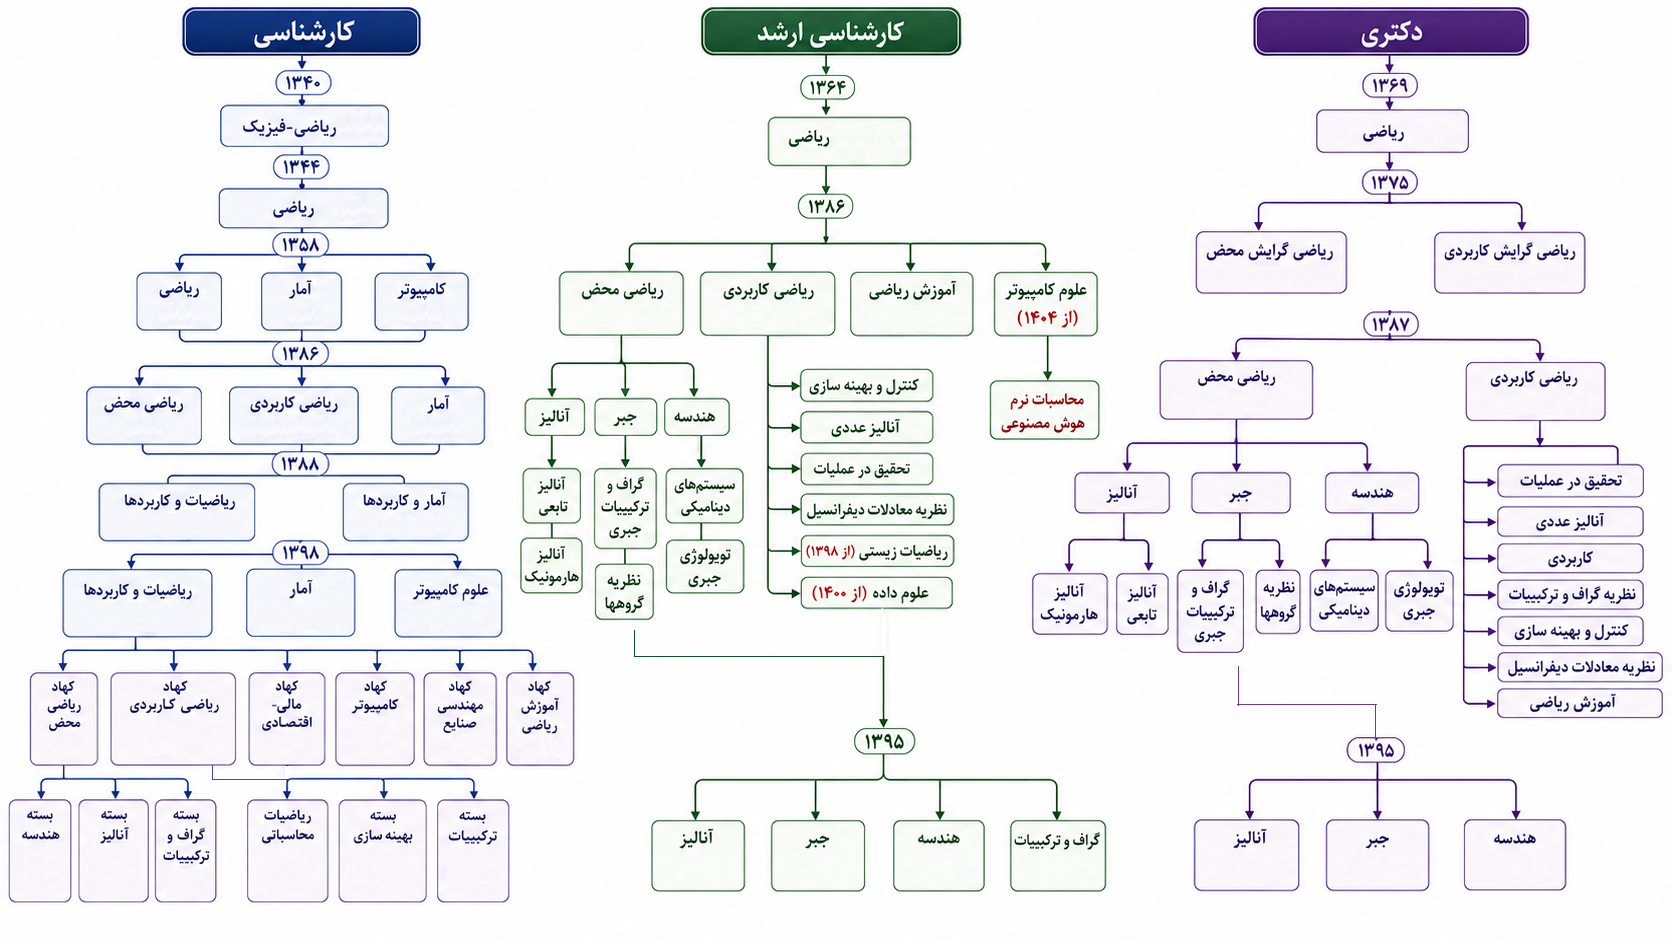
\includegraphics[keepaspectratio]{images/img_034.png}}

}

\caption{image}

\end{figure}%

\section{درختواره گروه
آمار}\label{ux62fux631ux62eux62aux648ux627ux631ux647-ux6afux631ux648ux647-ux622ux645ux627ux631}

\begin{figure}[H]

{\centering \pandocbounded{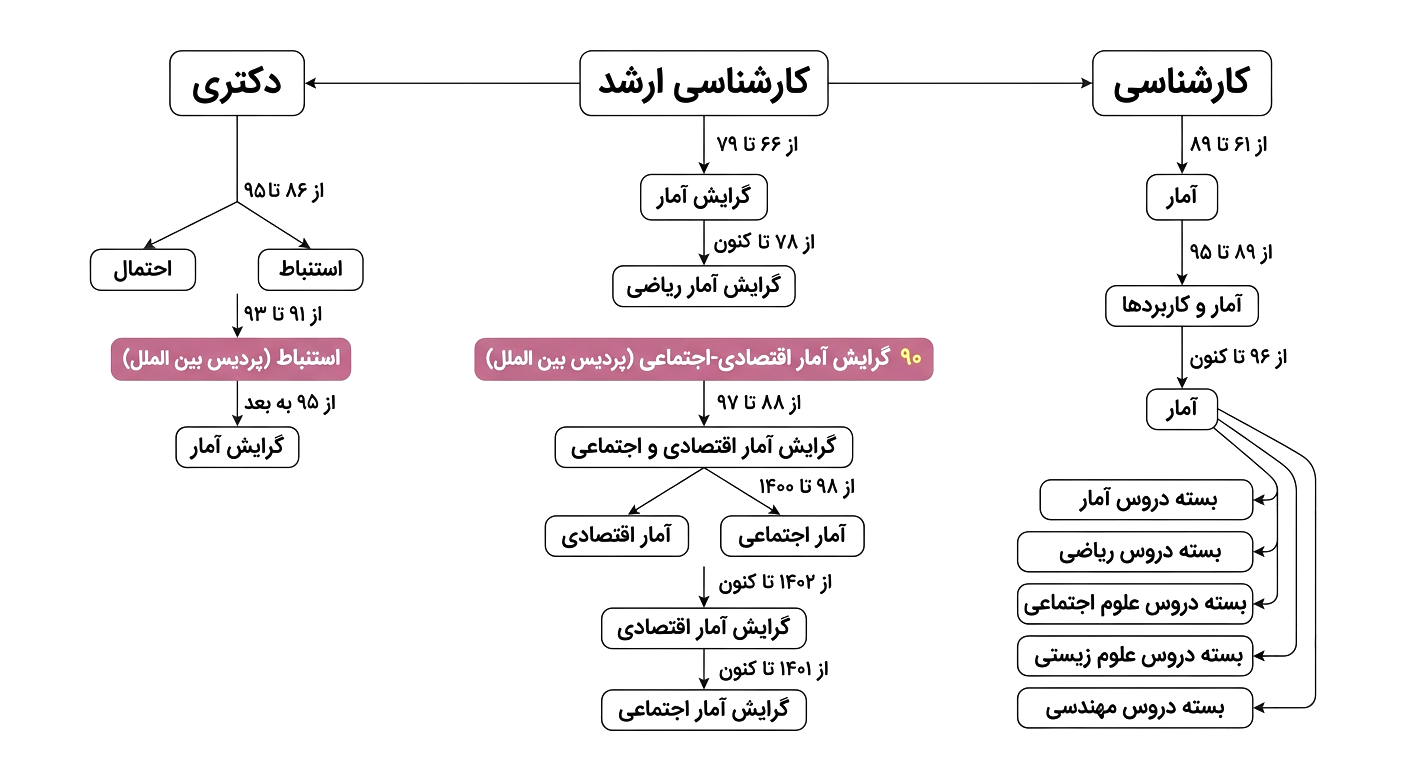
\includegraphics[keepaspectratio]{images/img_053.png}}

}

\caption{image}

\end{figure}%

\section{درختواره پردیس
بین‌الملل}\label{ux62fux631ux62eux62aux648ux627ux631ux647-ux67eux631ux62fux6ccux633-ux628ux6ccux646ux627ux644ux645ux644ux644}

\begin{figure}[H]

{\centering \pandocbounded{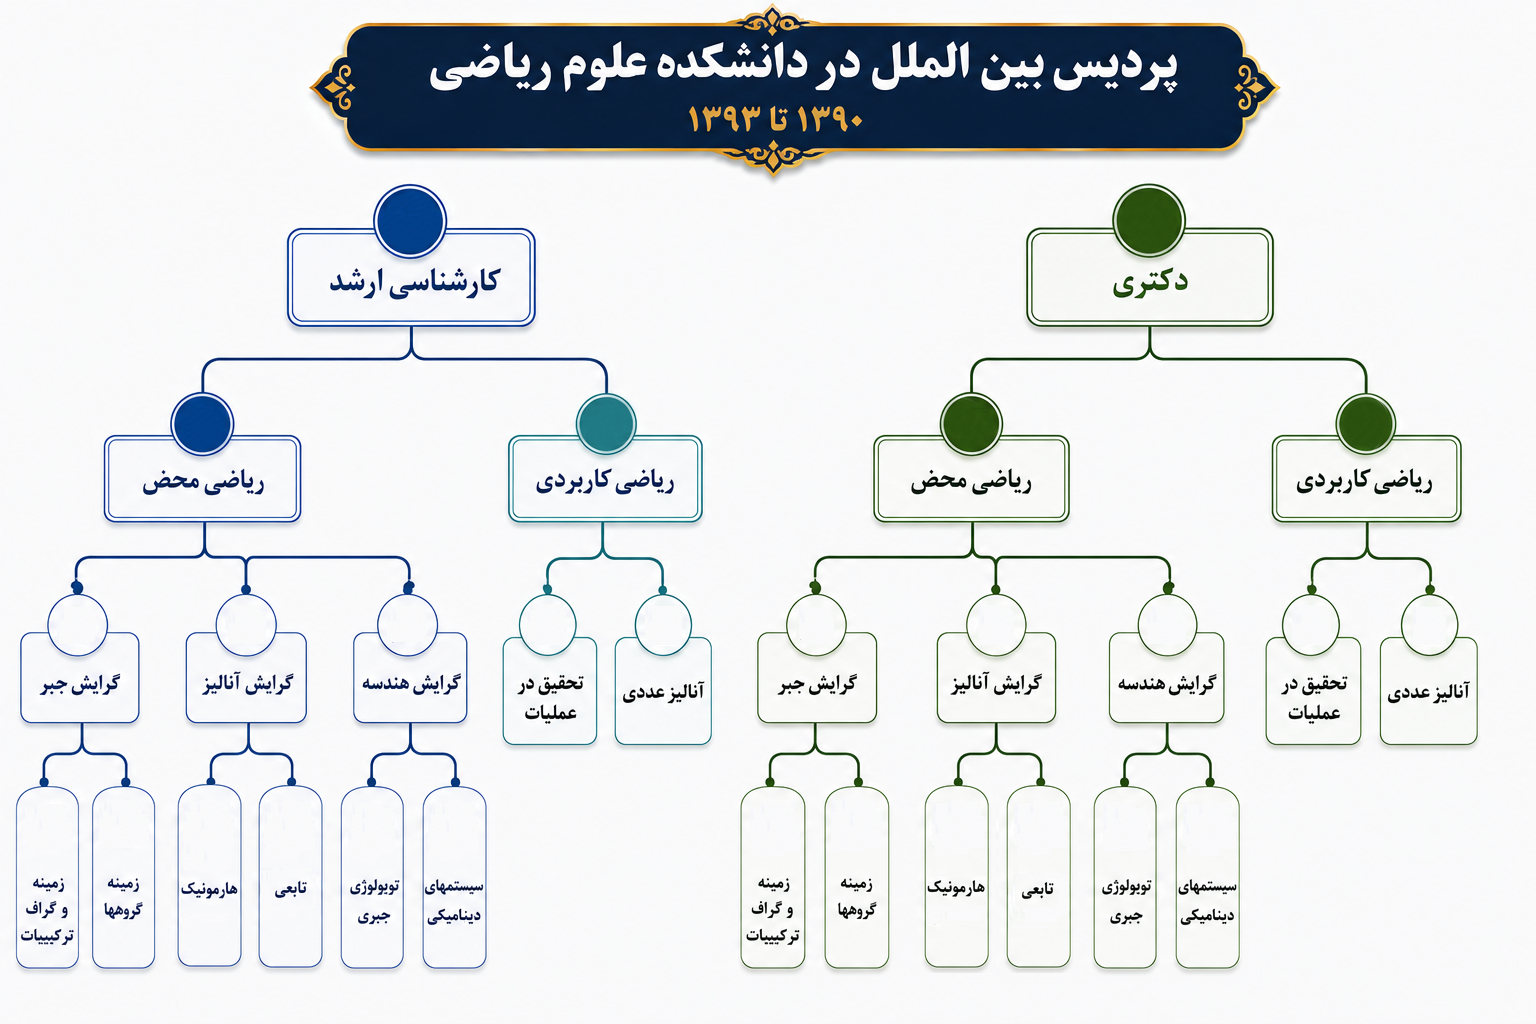
\includegraphics[keepaspectratio]{images/img_076.png}}

}

\caption{image}

\end{figure}%

\bookmarksetup{startatroot}

\chapter{مراجع}\label{ux645ux631ux627ux62cux639}

\bookmarksetup{startatroot}

\chapter{مراجع}\label{ux645ux631ux627ux62cux639-1}

منابع مورد استفاده در گردآوری این مجموعه، شامل اسناد بایگانی‌شده در
دانشکده علوم ریاضی، وب‌سایت‌های دانشگاه فردوسی مشهد، دانشکده علوم ریاضی و
کتابخانه مرکزی، وب سایت شخصی اعضای هیأت علمی و همچنین اطلاعات منتشرشده
در پایگاه‌های رسمی سازمان سنجش، انجمن ریاضی ایران و انجمن آمار ایران است.




\end{document}
